

\input{"/Users/brandonwilliams/Documents/LaTeX Includes/notespreamble.tex"}
\input{"/Users/brandonwilliams/Documents/LaTeX Includes/extrapackages.tex"}
\input{"/Users/brandonwilliams/Documents/LaTeX Includes/extracommands.tex"}


\begin{document}


\title{\Large Low Dimensional Topology}
\author{Brandon Williams \\ \texttt{mbw@math.sunysb.edu}}
\maketitle


\tableofcontents








\newpage
\section{Transversality and Intersection Theory}
\label{Transversality and Intersection Theory}




\subsection{Immersions, Submersions and Transversality}
\label{Immersions, Submersions and Transversality}


Let $f : M \rightarrow N$ be a smooth map between smooth manifolds. A point $p \in M$ is said to be \textbf{regular} if $df_p : T_p M \rightarrow T_{f(p)} N$ is surjective, otherwise it is said to be \textbf{critical}. The image of a critical point is called a \textbf{critical value}, and a \textbf{regular value} in $N$ is any point that is not a critical value. We say that $f$ is an \textbf{immersion} at $p \in M$ if $df_p$ is injective, and a \textbf{submersion} at $p \in M$ if $df_p$ is surjective. Recall the inverse function theorem and its corollaries pertaining to immersions and submersions. 
\begin{thm}[Inverse Function Theorem]
If $df_p : T_p M \rightarrow T_{f(p)} N$ is an isomorphism, then $f$ is a local diffeomorphism at $p$, i.e. there is a neighborhood $U$ of $p$ and $V$ of $f(p)$ such that $f|_U : U \rightarrow V$ is a diffeomorphism.
\end{thm}

\begin{cor}
If $f : M^m \rightarrow N^n$ is an immersion at $p \in M$, then there are coordinates $\phi : U \rightarrow \mathbb R^m$ around $p \in M$ and $\varphi : V \rightarrow \mathbb R^n$ around $f(p) \in N$ such that $\varphi \circ f \circ \phi^{-1}(x_1,\ldots,x_m) = (x_1,\ldots,x_m,0,\ldots,0)$.
\end{cor}
\begin{proof}
First let $\phi$ and $\varphi$ be any charts such that $\phi(p)=\varphi(p)=0$, and let $g = \varphi \circ f \circ \phi^{-1}$. Then $dg_0 : R^m \rightarrow R^n$ is injective since $f$ is an immersion, so we can change the coordinates so that
\[ dg_0 = \begin{pmatrix} I_m \\ 0 \end{pmatrix} \]
where $I_m$ is the $m \times m$ identity matrix and $0$ is the $(n-m) \times m$ zero matrix. We cannot apply the inverse function theorem to $g$ since $m < n$, but if we define $G : \phi(U) \times R^{n-m} \rightarrow R^n$ by $G(x,z) = g(x)+(0,z)$, then $dG_0 = I_n$. So $G$ is a local diffeomorphism, and $G \circ \varphi$ is another chart around $f(p)$ of $N$. In these coordinates we have that the local representation of $f$ is just $(x_1,\ldots,x_m) \mapsto (x_1,\ldots,x_m,0,\ldots,0)$. 
\end{proof}

\begin{cor}
\label{local submersion theorem}
If $f : M^n \rightarrow N^m$ is an submersion at $p \in M$, then there are coordinates $\phi : U \rightarrow \mathbb R^n$ around $p \in M$ and $\varphi : V \rightarrow \mathbb R^m$ around $f(p) \in N$ such that $\varphi \circ f \circ \phi^{-1}(x_1,\ldots,x_n) = (x_1,\ldots,x_m)$.
\end{cor}
\begin{proof}
First let $\phi$ and $\varphi$ be any charts such that $\phi(p)=\varphi(p)=0$, and let $g = \varphi \circ f \circ \phi^{-1}$. Then $dg_0 : R^n \rightarrow R^m$ is injective since $f$ is a submersion, so we can change the coordinates so that
\[ dg_0 = \begin{pmatrix} I_m & 0 \end{pmatrix} \]
where $I_m$ is the $m \times m$ identity matrix and $0$ is the $m \times (n-m)$ zero matrix. We cannot apply the inverse function theorem to $g$ since $m < n$, but if we define $G : R^n \rightarrow \varphi(V) \times R^{n-m}$ by $G(x_1,\ldots,x_n) = (g(x),x_{m+1},\ldots,x_n)$, then $dG_0 = I_n$. So $G$ is a local diffeomorphism, and $G^{-1} \circ \phi$ is another chart around $p$ of $M$. In these coordinates we have that the local representation of $f$ is just $(x_1,\ldots,x_n) \mapsto (x_1,\ldots,x_m)$. 
\end{proof}

\begin{cor}
\label{pre-image of regular value is submanifold}
If $q$ is a regular value of $f : M^n \rightarrow N^m$, then $f^{-1}(q)$ is a submanifold of $M$ with $\codim f^{-1}(q) = m$.
\end{cor}
\begin{proof}
Let $p \in f^{-1}(q)$, then $f$ is a submersion at $p$, so by \cref{local submersion theorem} we can find coordinates $\phi : U \rightarrow \mathbb R^n$ around $p$ and $\varphi : V \rightarrow \mathbb R^m$ around $q$ such that $\varphi \circ f \circ \phi^{-1}(x_1,\ldots,x_n)=(x_1,\ldots,x_m)$ and $\varphi(q)=(0,\ldots,0)$. Thus for $x \in U$ and $f(x)=q$ we have $\phi(x)=(0,\ldots,0,x_{m+1},\ldots,x_n)$ for some $x_{m+1},\ldots,x_n$. So $\phi$ restricted to $U \cap f^{-1}(q)$ provides a chart of the relatively open set $U \cap f^{-1}(q)$ into $\mathbb R^{n-m}$, making $f^{-1}(q)$ into a submanifold of dimension $n-m$.
\end{proof}

Consider the following simple application of \cref{pre-image of regular value is submanifold}. For real-valued functions $f_1,\ldots,f_k : M \rightarrow \mathbb R$, when is the set $Z$ of common zeros a manifold? If we set $f = (f_1,\ldots,f_k) : M \rightarrow \mathbb R^k$, then it is clear that $f^{-1}(0)$ is a manifold if $0$ is a regular value of $f$. Another way of looking at this is to see that $df_p = ((df_1)_p,\ldots,(df_k)_p) : T_p M \rightarrow T_{f(p)} \mathbb R^k$, and this is surjective if and only if $(df_1)_p,\ldots,(df_k)_p$ are linearly independent functionals. When this happens we say $f_1,\ldots,f_k$ are independent at $p$, and so we have the following corollary.
\begin{cor}
If $f_1,\ldots,f_k : M \rightarrow \mathbb R$ are independent at all points where they simultaneously vanish, then the set of common zeros $Z$ is a submanifold with $\dim Z = \dim M - k$.
\end{cor}

In the case of the above corollary we say that the submanifold $Z$ has been \emph{cut out} by the functions $f_1,\ldots,f_k$. However, not every submanifold can be globally cut out by independent functions. 

Now that we know the pre-image of regular values are submanifolds, we naturally wonder if the pre-image of \emph{submanifolds} are submanifolds. Two smooth maps $f : M \rightarrow N$ and $g : L \rightarrow N$ are said to be \textbf{transversal} if at any point $p \in M$ and $q \in L$ for which $f(p)=g(q)$ we have
\[ df_{p}(T_p M) + dg_{q}(T_q N) = T_{f(p)} N \]
and we denote this by $f \pitchfork g$. Note that the above sum does \emph{not} have to be direct, and in fact most of the time will not be. If $g$ is just the inclusion of a submanifold $L$ of $N$, then we say $f$ is transverse to $L$ and write $f \pitchfork L$. If $f$ is also an inclusion of a submanifold $M$ of $N$, then we say the submanifolds $M$ and $L$ are transversal, and write $M \pitchfork L$.
\begin{prop}
\label{pre-image of submanifold under transversality}
If $f : M \rightarrow N$ is transverse to a submanifold $L$ in $N$, then $f^{-1}(L)$ is a submanifold of $M$ with $\codim f^{-1}(L) = \codim L$. In particular, if two submanifolds $M$ and $L$ of $N$ are transversal, then $M \cap L$ is another submanifold of $N$ and $\codim(M \cap L) = \codim M + \codim L$.
\end{prop}


An important feature of immersions, submersions, transversal intersections and embeddings is that they can be ``perturbed'' slightly, and they will remain in their respective class. To make this precise we need to define what we mean by perturbation. Fix a smooth map $f_0 : M \rightarrow N$, and let $F : M \times [-1,1] \rightarrow N$ be a smooth map such that $F(-,0) = f_0$. In fact, we will use the notation $f_t = F(-,t)$. Then any of the smooth maps $f_t : M \rightarrow N$ for $t \in [-1,1]$ are called \textbf{smooth perturbations} of $f_0$; that is, we just smoothly homotoped $f_0$ a little bit. We say that a statement $P$ defined on the space of smooth functions $C^\infty(M,N)$ is \textbf{stable} if for every $f \in C^\infty(M,N)$ such that $P(f)$ and every family of perturbations $F$ of $f$, then there is a small enough $\epsilon$ such that $P(f_t)$ for all $|t| < \epsilon$.

\begin{thm}
\label{stability theorem}
Let $M$ be compact. The following statements are stable as statements on $C^\infty(M,N)$.
\begin{enumerate}
	\item $P(f) = f$ is an immersion.
	\item $P(f) = f$ is an submersion.
	\item $P(f) = f$ is a local diffeomorphism.
	\item For a fixed submanifold $Z \subset N$, $P(f) = f$ is transversal to $Z$.
	\item $P(f) = f$ is an embedding.
	\item $P(f) = f$ is an diffeomorphism.
\end{enumerate}
\end{thm}
\begin{proof}
\sloppyspace
\begin{enumerate}

	\item Suppose $f_0 : M^m \rightarrow N^n$ is an immersion, and take a family $F : M \times [-1,1] \rightarrow N$ perturbations of $f_0$, i.e. $F(-,0)=f_0$. The result will follow if we prove every point $(x,0) \in M \times [-1,1]$ has an open neighborhood $U_x$ such that $df_p$ is injective for all $p \in U$. For then we can take their union $U = \cup_x U_x$ and choose an $\epsilon>0$ small enough so that $M \times (-\epsilon,\epsilon) \subseteq U$. Since this is now just a local question we might as well assume $M$ is an open subset of $\mathbb R^m$ and $N$ is an open subset of $\mathbb R^n$. Since $(df_0)_x$ is injective, we have that the Jacobian matrix $(\partial (f_0)_i / \partial x_j(x))_{ij}$ contains at least $m$ linearly independent columns. We can of course assume that these columns are the first $m$ columns of the Jacobian. If we consider the Jacobian as a function of $(x,t) \in X \times [-1,1]$, then we see that the determinant of the first $m$ columns is a smooth function that is not equal to zero at $(0,x)$, hence we can find an $\epsilon>0$ small enough so that it is not zero for $(t,x)$, $|t|<\epsilon$. Therefore all the $f_t$'s are immersions for $|t|<\epsilon$.
	
	\item The proof of this identical to 1 as now the Jacobian has $n$ linearly independent rows.
	
	\item This follows directly from 1 since a local diffeomorphism is just an immersion for when $\dim M = \dim N$.
	
	\item The condition of being transverse has an equivalent reformulation in terms of local submersions, so this follows from 2.
	
	\item Recall that an embedding is a proper, injective immersion $f_0 : M \rightarrow N$. Since $M$ is compact, $f_0$ is automatically proper, so we only need to prove that if $f_0$ is injective, then $f_t$ is injective for $|t|$ less than some small $\epsilon>0$. We prove this by contradiction, so we can assume there is a sequence of numbers $t_i \to 0$ and distinct points $x_i \neq y_i$ such that $f_{t_i}(x_i) = f_{t_i}(y_i)$. Since $M$ is compact we can pass to a subsequence such that $t_i \to 0$, $x_i \to x$, and $y_i \to y$. If we define the function $G : M \times I \rightarrow N \times I$, then we have $G(x_i,t_i)=G(y_i,t_i)$ (by definition), hence
	\[ G(x,0) = \lim_{i\to\infty} G(x_i,t_i) = \lim_{i\to\infty} G(y_i,t_i) = G(y,0) \]
	Since $f_0$ is injective this implies $x=y$. The Jacobian of $G$ at $(x,0)$ is in block form
	\[ \begin{pmatrix} & & & * \\ & d(f_0)_x & & \vdots \\ & & & * \\ 0 & \cdots & 0 & 1 \end{pmatrix} \]
	But, $d(f_0)_x$ is injective, hence $dG_{(x,0)}$ has at least $m+1$ linearly independent columns and so $G$ is an immersion at $(x,0)$. This will remain true in a small neighborhood of $(x,0)$, which must contain the points $(x_i,t_i)$ and $(y_i,t_i)$ for large enough $i$. This contradicts that $G(x_i,t_i)=G(y_i,t_i)$, therefore no such sequence can exist, and so $f_t$ is injective for $|t|$ small enough.
	
	\item 
	
\end{enumerate}
\end{proof}


Now let us extend the ideas of transversality to manifolds with boundary. For a manifold $M$ with boundary, and a smooth map $f : M \rightarrow N$, the restriction of $f$ to the boundary $\partial M$ will be denoted by $\partial f$. 


\unfinished






\subsection{Intersection Theory}
\label{Intersection Theory}

Recall the following classification of 1-dimensional manifolds and one of its immediate corollaries.
\begin{prop}
Every compact 1-dimensional manifold is homeomorphic to a disjoint union of circles and closed intervals.
\end{prop}
\begin{cor}
The number of boundary components of any compact 1-dimensional manifold is even.
\end{cor}

Consider a smooth map $f : M \rightarrow N$, with $M$ compact, and submanifold $Z \subseteq M$. By slightly perturbing $f$, if necessary, we can assume $f \pitchfork Z$ and so $f^{-1}(Z)$ is a submanifold of $M$. If $\codim Z = \dim M$, then $\codim f^{-1}(Z) = \codim Z = \dim M$, hence $f^{-1}(Z)$ is a 0-dimensional manifold. Since $M$ is compact, $f^{-1}(Z)$ consists of finitely many points, so we define the \textbf{mod-2 intersection number} of $f$ and $Z$ by $I_2(f,Z) = \#f^{-1}(Z) \modulo 2$. This is well-defined by the following proposition.
\begin{prop}
If $f,g : M \rightarrow N$ are homotopic, then $I_2(f,Z) = I_2(g,Z) \modulo 2$.
\end{prop}
\begin{proof}
Let $F : M \times I \rightarrow N$ be a homotopy between $f$ and $g$. We can perturb $F$ slightly, while keeping $F_0$ and $F_1$ fixed, to make $F \pitchfork Z$. Then $F^{-1}(Z)$ is a submanifold of $M \times I$ with $\codim F^{-1}(Z) = \codim Z = \dim M$, hence $\dim F^{-1}(Z)=1$. The boundary of $F^{-1}(Z)$ consists of
\[ F^{-1}(Z) \cap \partial (M \times I) = F^{-1}(Z) \cap (M \times \lcb 0 \rcb \cup M \times \lcb 1 \rcb) = f^{-1}(Z) \times \lcb 0 \rcb \cup g^{-1}(Z) \times \lcb 1 \rcb \]
Since $\# \partial F^{-1}(Z)$ is even, we must have that $\# f^{-1}(Z)$ and $\# g^{-1}(Z)$ are both even or both odd, hence $I_2(f,Z) = I_2(g,Z) \modulo 2$.
\end{proof}
We can define the mod-2 intersection number of two submanifolds $W,Z \subseteq M$ as $I_2(W,Z) := I_2(i,Z)$ where $i : W \hookrightarrow M$ is the inclusion. Although we can slightly perturb $W$ and $Z$ to create more intersection points (or remove intersection points), the above proposition says that points must be added in pairs.



\unfinished







\newpage
\section{Knot Theory}
\label{Knot Theory}


One of the reasons that low dimensional topology is so much harder to study than higher dimensions is the appearance of knots. In high dimensions one can unravel all knots to become ``trivial,'' but this does not happen in 3 dimensions. Fortunately we can get a combinatorial presentation of 3-manifolds from knots, but before that we have to cover some basics of knot theory.


\subsection{Basic Definitions}
\label{Basic Definitions}


Classically, a \textbf{knot} $k$ is just a smoothly embedded copy of $S^1$ into $S^3$. We could also embed our knots into $\mathbb R^3$, the theories would turn out to be equivalent, but $S^3$ is easier to think about since it is a nice compact 3-manifold. The complement of a knot in its surrounding manifold is called the \textbf{knot complement}, and its first homology group is quite simple.

\begin{prop}
\label{homology of knot complement in sphere}
If $k$ is a knot in $S^3$, then $H_1(S^3 \backslash k) = \mathbb Z$ and is generated by any meridian.
\end{prop}
\begin{proof}
Let $U$ be an open tubular neighborhood of $k$ in $S^3$, and let $V$ be the complement of the closure of a \emph{smaller} tubular neighborhood. Then $U$ is homotopy equivalent to $S^1$, $V$ is homotopy equivalent to the knot complement $S^3 \backslash k$, and $U \cap V$ is homotopy equivalent to a torus $S^1 \times S^1$. The Mayer-Vietoris sequences gives us the following exact sequence
\[ 0 \longrightarrow H_1(U \cap V) \stackrel{}{\longrightarrow} H_1(U) \oplus H_1(V) \stackrel{}{\longrightarrow} 0 \]
which is just
\[ 0 \longrightarrow \mathbb Z \oplus \mathbb Z \longrightarrow \mathbb Z \oplus H_1(S^3 \backslash k) \longrightarrow 0 \]
This implies that $H_1(S^3 \backslash k) = \mathbb Z$. Further, note that this map is of the form $(i_*,-j_*)$, where $i$ and $j$ are the inclusions of $U \cap V$ into $U$ and $V$, respectively. The group $H_1(U \cap V) = \mathbb Z \oplus \mathbb Z$ is generated by a meridian $[\mu]$ and longitude $[\ell]$, and we can choose this longitude such that $j_*[\ell]=0$. Since $[\ell]$ is mapped to an element generating the first factor of $\mathbb Z \oplus H_1(S^3 \backslash k)$, we have that $j_*[\mu]$ generates the second factor.
\end{proof}


%%%%%%%%%%%%%%%%%%%%%%%%%%%%%%%%%%%%%%%%%
%%%%%%%%%%%%%%%%%%%%%%%%%%%%%%%%%%%%%%%%%
%%%%%%%% TRY TO FINISH LATER %%%%%%%%%%%%
%%%%%%%%%%%%%%%%%%%%%%%%%%%%%%%%%%%%%%%%%
%%%%%%%%%%%%%%%%%%%%%%%%%%%%%%%%%%%%%%%%%
\comment{
\begin{prop}
\label{homology of knot complement in sphere}
If $k$ is a knot in $S^3$, then $H_n(S^3 \backslash k) = \mathbb Z$ for $n=0,1$ and $=0$ for $n \geq 2$.
\end{prop}
\begin{proof}
Since $S^3 \backslash k$ is a connected, non-compact 3-manifold, we already have $H_0(S^3 \backslash k) = \mathbb Z$ and $H_k(S^3 \backslash k) = 0$ for $k \geq 3$. Let $U$ be an open tubular neighborhood of $k$ in $S^3$, and let $V$ be the complement of the closure of a \emph{smaller} tubular neighborhood. Then $U$ is homotopy equivalent to $S^1$, $V$ is homotopy equivalent to the knot complement $S^3 \backslash k$, and $U \cap V$ is homotopy equivalent to a torus $S^1 \times S^1$. The Mayer-Vietoris sequence gives us the following exact sequences
\[ 0 \longrightarrow H_3(S^3) \stackrel{\Delta}{\longrightarrow} H_2(U \cap V) \stackrel{}{\longrightarrow} H_2(U) \oplus H_2(V) \stackrel{}{\longrightarrow} 0 \]
\[ 0 \longrightarrow H_1(U \cap V) \stackrel{}{\longrightarrow} H_1(U) \oplus H_1(V) \stackrel{}{\longrightarrow} 0 \]
The first exact sequence is really just
\[ 0 \longrightarrow \mathbb Z \stackrel{\Delta}{\longrightarrow} \mathbb Z \longrightarrow H_2(S^3 \backslash k) \longrightarrow 0 \]
To see that the connecting morphism $\Delta$ is an isomorphism recall how it is defined. Every homology class $\omega \in H_3(M)$ can be represented by a cycle of the form $c+d$, where $c$ and $d$ are cycles in $U$ and $V$ respectively. Since $\partial c = -\partial d$ we see that the image of $\partial c$ is contained in $U \cap V$. So we define $\Delta \omega = [\partial c] \in H_2(U \cap V)$. \unfinished

Whereas the second exact sequence is really just
\[ 0 \longrightarrow \mathbb Z \oplus \mathbb Z \longrightarrow \mathbb Z \oplus H_1(S^3 \backslash k) \longrightarrow 0 \]
Therefore $\mathbb Z^2 \cong \mathbb Z \oplus H_1(S^3 \backslash K)$, hence $H_1(S^3 \backslash k) = \mathbb Z$.
\end{proof}
}
%%%%%%%%%%%%%%%%%%%%%%%%%%%%%%%%%%%%%%%%%
%%%%%%%%%%%%%%%%%%%%%%%%%%%%%%%%%%%%%%%%%
%%%%%%%% /TRY TO FINISH LATER %%%%%%%%%%%
%%%%%%%%%%%%%%%%%%%%%%%%%%%%%%%%%%%%%%%%%
%%%%%%%%%%%%%%%%%%%%%%%%%%%%%%%%%%%%%%%%%

Given two knots $k_1,k_2$ in a manifold $S^3$, we say that they are \textbf{equivalent}, or \textbf{isotopic}, if they are ambiently isotopic. This means that there is a smooth 1-parameter family of maps $\varphi_t : S^3 \rightarrow S^3$ such that $\varphi_0 = \id$, $\varphi_1(k_1)=k_2$, and $\varphi_t$ is a diffeomorphism for all time $t$. A knot that is isotopic to the standardly embedded $S^1$ in $S^3$ is called the \textbf{unknot} or the \textbf{trivial knot}.

There is a nice way to visualize a knot $k$ in $S^3$. First, move the knot a little if needed so that it does not pass through the point at infinity. Now $k$ is embedded in $\mathbb R^3$. For a generic plane $\Pi$ in $\mathbb R^3$ not intersecting $k$, the projection $D$ of $k$ onto $\Pi$ is a closed curve with finitely many double points, and no other types of singularities. We can decorate these double points as an over or under crossing depending on whether one strand is above another relative to the plane. Such a projection $D$ is called a \textbf{knot diagram} of $k$. Conversely, given a closed curve $D$ in the plane which is embedded on the complement of finitely many double points and whose double points are decorated with under or over crossings, we can find a knot $k$ such that $D$ is a projection of $k$. 

Clearly a single knot $k$ can admit many different knot diagrams, and so we hope there is a way to determine when two diagrams correspond to the same isotopy class of knot. It turns out there are 3 moves one can apply to a knot diagram, called the \textbf{Reidemeister moves}, such that two knot diagrams $D_1$ and $D_2$ are the diagrams of two isotopic knots if and only if one can get from one diagram to the other by the Reidemeister moves (see \cref{reidemeister moves}). We will use $R_1,R_2$ and $R_3$ to denote these moves. This reduces a lot of knot theory to combinatorial pictures, from which we can define a lot of knot invariants. 

\begin{figure}[tb]
\centering
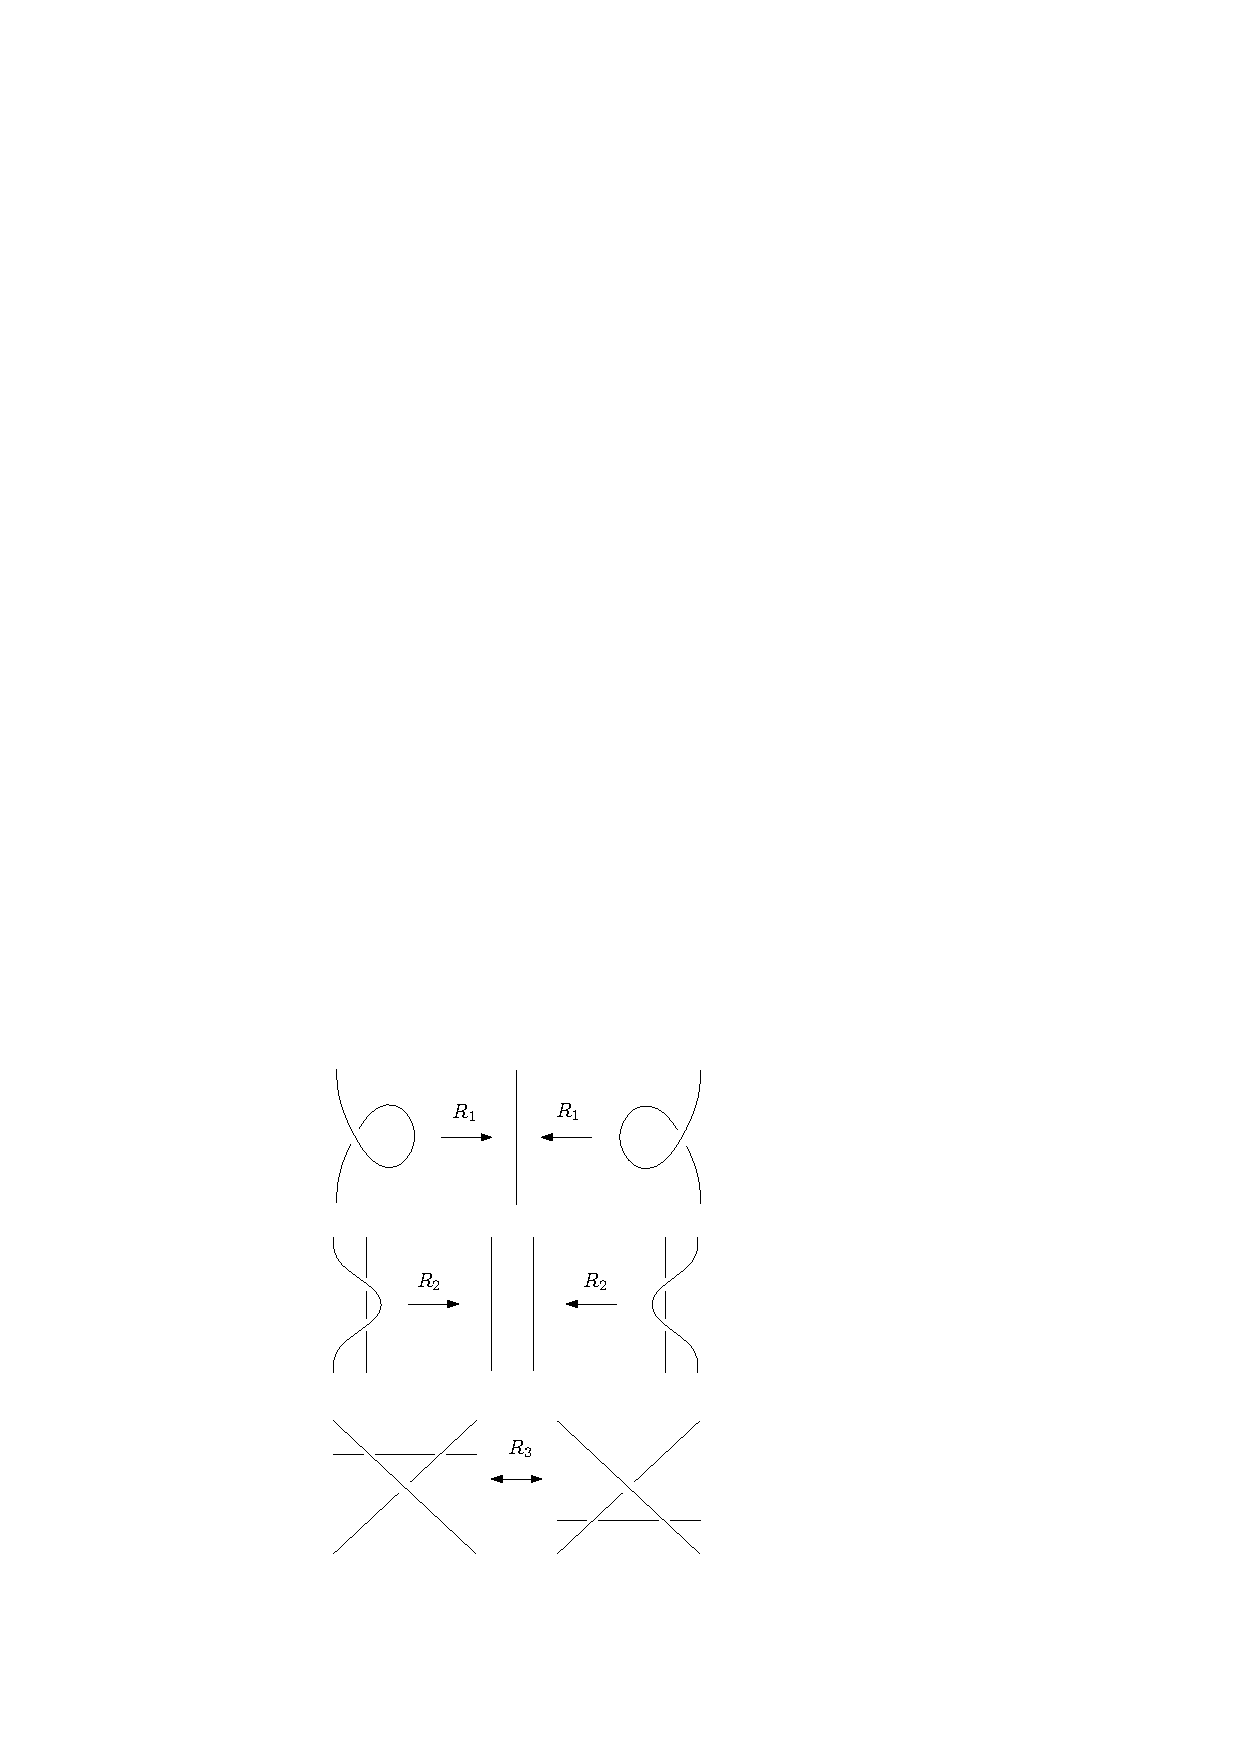
\includegraphics[scale=1]{graphics/reidemeister-moves}
\caption{Reidemeister Moves}
\label{reidemeister moves}
\end{figure}

A slight generalization of a knot is a link. An \textbf{$n$-component link} is a smooth embedding of $n$ copies of $S^1$. All of the above definitions and discussion has a direct generalization to links. Clearly if two links $L_1$ and $L_2$ are isotopic, then their number of components must be equal.

One can put an orientation on a knot $k$ by simply choosing a non-vanishing tangent vector field on $k$, or equivalently placing an arrow on any knot diagram of $k$. A knot has precisely 2 orientations and an $n$-component link has $2^n$ orientations. Given a knot diagram $D$ of an oriented knot $k$, we can define the \textbf{sign} of each crossing of $D$. We adopt the right hand rule for sign conventions, which means signs are determined as in \cref{crossing signs}. Note that the sign of a crossing is information we get once we have chosen a knot diagram, not from just a knot. The sum of all the signs of the crossing of a knot diagram $D$ is called the \textbf{writhe} of the diagram, and is denoted by $w(D)$. The writhe of a knot diagram is \emph{not} a knot invariant because it is not invariant under $R_1$. It is, however, a ribbon invariant, but we will not discuss that here.

\begin{figure}[tb]
\centering
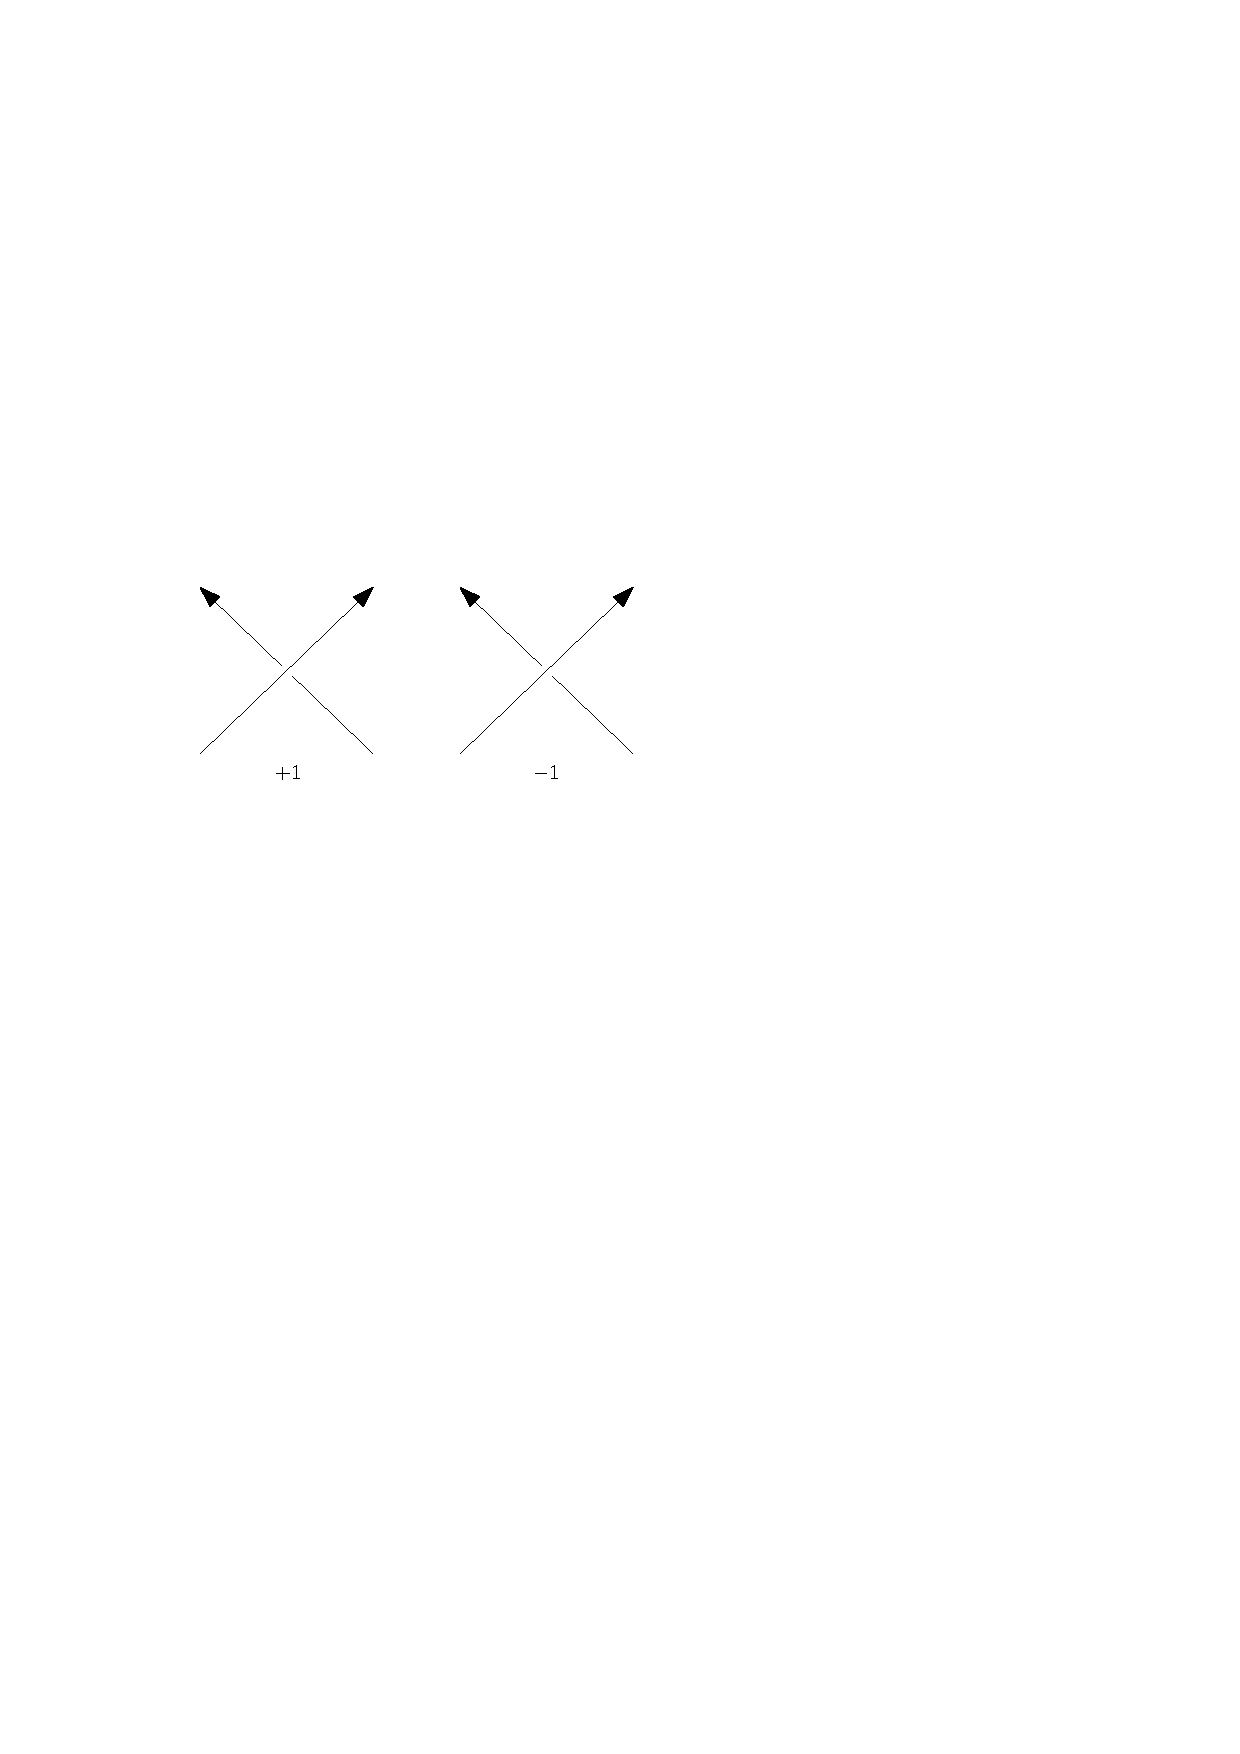
\includegraphics[scale=1]{graphics/crossing-signs}
\caption{Crossing Signs}
\label{crossing signs}
\end{figure}

Let $k$ be a knot in $S^3$ and $D$ a diagram of $k$. A \textbf{resolution of a crossing}, or a \textbf{smoothing}, is the process of removing the double point and reconnecting the strands so that there is no crossing. There are two ways of doing this, called the 0-resolution and 1-resolution, shown in \cref{crossing resolution}. Each time one resolves a crossing the number of components of the diagram either stays the same or increases by one. A \textbf{resolution of a diagram} is the diagram resulting from resolving all crossings, which is just a finite collection of disjoint circles. Clearly if there are $n$ crossings in the diagram $D$, then there are $2^n$ resolutions, which are parameterized by $\lcb 0,1 \rcb^n$. If the knot $k$ has an orientation, then there is a canonical resolution of $D$, called the \textbf{oriented resolution}, where we resolve all the crossings of sign $+1$ by a 1-resolution and all crossings of sign $-1$ by a 0-resolution. 


\begin{figure}[tb]
\centering
\[
\xy0;/r0.4pc/:
(-6,6)*{}="tl";
(6,6)*{}="tr";
(-6,-6)*{}="bl";
(6,-6)*{}="br";
"tl";"tr" **\crv{(0,1)};
"bl";"br" **\crv{(0,-1)};
(0,-10)*{\text{0-resolution}};
\endxy
\qquad \qquad
\xy0;/r0.4pc/:
(6,6)*{}="tl";
(-6,6)*{}="tr";
(6,-6)*{}="bl";
(-6,-6)*{}="br";
{\ar@{-}|{\hole \; \hole \; \hole \; \hole \; \hole \; \hole } "bl";"tr"};
{\ar@{-} "br";"tl"};
(0,-10)*{\text{crossing}};
\endxy
\qquad \qquad
\xy0;/r0.4pc/:
(-6,6)*{}="tl";
(6,6)*{}="tr";
(-6,-6)*{}="bl";
(6,-6)*{}="br";
"bl";"tl" **\crv{(-1,0)};
"br";"tr" **\crv{(1,0)};
(0,-10)*{\text{1-resolution}};
\endxy 
\]
\caption{Ways to resolve a crossing}
\label{crossing resolution}
\end{figure}

A \textbf{Seifert surface} for a link $L$ in $S^3$ is a smoothly embedded, compact, connected and orientable surface $F$ in $S^3$ with boundary such that $\partial F = L$. 
\begin{prop}[Seifert's Algorithm]
\label{Seifert's algorithm}
Every link $L$ in $S^3$ has a Seifert surface.
\end{prop}
\begin{proof}
We can construct the surface explicitly. Choose any orientation on $L$ and let $D$ be a diagram for $L$. Let $D'$ denote the the oriented resolution of $D$. Fill each component of $D'$ so that there is a disc for each circle, and connect the discs a twisting band for each crossing. The result is a surface with boundary equal to exactly $L$.
\end{proof}

Any link has many Seifert surfaces, and Seifert's algorithm almost never produces the surface of minimal genus. We define the \textbf{genus} of a link $L$ to be the minimum of genera of Seifert surfaces of $L$, and is denoted by $g(L)$. The \textbf{four-ball genus} of $L$ is the minimum of genera of compact, connected, oriented and smoothly embedded surfaces in $D^4$ whose boundary is $L \subset \partial D^4 = S^3$, and is denoted by $g^*(L)$.

\begin{lem}
\label{additivity of genus}
Let $k_1,k_2$ be two knots embedded in $S^3$. Then the genus satisfies $g(k_1 \# k_2) = g(k_1) + g(k_2)$.
\end{lem}
\begin{proof}
We can think of $k_1$ and $k_2$ embedded in the same sphere, but situated far apart. Let $F_1$ and $F_2$ be Seifert surfaces of minimal genus for $k_1$ and $k_2$, respectively. Then the boundary sum $F_1 \sharp F_2$ is a Seifert surface of $k_1 \# k_2$, and so we have proved
\[ g(k_1 \# k_2) \leq g(k_1) + g(k_2) \]

To prove the other inequality we fix a Seifert surface $F$ of minimal genus for $k_1 \# k_2$. We can fix a 2-sphere $\Sigma$ in $S^3$ so that $\Sigma \cap k_1 \# k_2$ consists of two points. Then, if the two arcs of $k_1 \# k_2$ between these two points are labelled $\alpha_1$ and $\alpha_2$, and we take a small arc $\beta$ in $\Sigma$ between these two points, then the curve $\alpha_1 + \beta$ is $k_1$ and the curve $\alpha_2 + \beta$ is $k_2$. By perturbing $\Sigma$ slightly we can guarantee that $\Sigma \cap F$ is just a collection of closed curves, as well as the curve $\beta$. We will perform surgery on these closed curves one by one to remove these intersections, so that the only intersection points left is the arc $\beta$.

Let $C$ be one of these closed curves with the additional property that the disc it bounds in $\Sigma$ does not contain any of the other closed curves. These ensures that if we push the interior of this disc a little off of $\Sigma$ (in either direction) it does not intersect $F$. Let $\hat F$ be the surface obtained from $F$ by cutting out an open annulus around $C$ (so now there are two more boundary components) and gluing in two discs, each parallel to the disc in $\Sigma$ bounded by $C$, and on either side of $\Sigma$. The result is another Seifert surface $\hat F$ of $k_1 \# k_2$. If the curve $C$ does not separate $F$, then $\hat F$ will have genus one less that $F$ (we just cut open a handle!), which is not possible since $F$ is assumed to have minimal genus. So, we must have that $C$ separates $F$, hence $\hat F$ consists of a disjoint union of a 2-sphere and a Seifert surface of $k_1 \# k_2$ that has one less intersection with $\Sigma$. Repeating this for all the closed curves in $\Sigma \cap F$ shows that we can assume that $\Sigma$ and $F$ intersect only at the arc $\beta$. 

Now we can take $F_1$ to be the closure of the part of $F$ outside of the sphere $\Sigma$, and $F_2$ the closure of the part of $F$ inside the sphere. Then $F_1$ and $F_2$ are Seifert surfaces of $k_1$ and $k_2$ respectively, hence
\[ g(k_1) + g(k_2) \leq g(k_1 \# k_2) \]
\end{proof}

Given disjoint, oriented knots $k_1$ and $k_2$, let $D$ be a common projection. We can assign signs to the double points of $D$ just as before, except now the two strands might belong to different knots. The \textbf{linking number} $\lk(k_1,k_2)$ of $k_1$ and $k_2$ is defined to be the sum of the signs of all crossings where $k_1$ passes under $k_2$. In order to show that this definition is well-defined we need to see that it does not depend on the diagram chosen for $k_1 \cup k_2$. It is an easy matter to show that $\lk(k_1,k_2)$ is invariant under the Reidemeister moves, hence $\lk(k_1,k_2)$ is an invariant of the isotopy class of $k_1 \cup k_2$. It is also easy to check that $\lk(k_1,k_2)=\lk(k_2,k_1)$ and $\lk(-k_1,k_2) = -\lk(k_1,k_2)$, where $-k_1$ is the knot $k_1$ with opposite orientation. 

There are two other ways of describing the linking number that will be useful later. Let $L = k_1 \cup k_2$ be the link with components our knots, and let $F$ be a Seifert surface for $L$. At each point on the boundary $k_1$ in $F$ we have a tangent vector $\tau$ that determines the orientation of $k_1$ and a vector $\nu$ pointing into the surface. Let $n$ be a vector normal to $F$ such that the ordered basis $(\tau,\nu,n)$ matches with the orientation of $S^3$. The normal vector $n$ can be extended to the rest of the surface $F$, and it determines an orientation. We can perturb $k_2$ slightly if needed so that $k_2$ intersects $L$ transversely in finitely many points. If we assign these points the sign $+1$ when $k_2$'s tangent vector points in the same direct as $n$ and $-1$ when it points in the opposite direction, then $\lk(k_1,k_2)$ is equal to the sum of these numbers. 

The second way is to notice that the first homology of the knot complement $H_1(M\backslash k_1) = \mathbb Z$ is generated by the homology class $[\mu]$ of any meridian $\mu$ of $k_1$. The other knot $k_2$ determines a homology class $[k_2] \in H_1(M\backslash k_1)$, which must be an integer multiple of $[\mu]$. The linking number $\lk(k_1,k_2)$ is precisely this number, i.e. $[k_2] = \lk(k_1,k_2) \cdot [\mu]$. 

A \textbf{framing} for a knot $k$ in $S^3$ is a choice of a normal vector field along $k$. If $X$ is a framing of $k$, then we can push $k$ a little bit in the direction of $X$ to get a new knot $k'$, and the integer $\lk(k,k')$ is called the \textbf{framing number} or \textbf{framing coefficient} of $X$. Conversely, given an integer $n$ we can find a parallel $k'$ of $k$ such that $\lk(k,k')=n$, and this curve is unique up to isotopy in $S^3 \backslash k$. So, we can think of framings as either normal vector fields, parallel knots, or just integers assigned to knots. A knot with a framing is called a framed knot, and a framed link is defined similarly. For an oriented, framed link $L$ with components $L_1,\ldots,L_n$ we define its \textbf{linking matrix} $[L]$ to be the symmetric matrix with $(i,j)$-entry equal to $\lk(L_i,L_j)$, where we use the convention that $\lk(L_i,L_i)$ is just the framing of the $i$-th component of $L$.

Given a knot $k$ in $S^3$ the meridian $\mu$ of $\partial N(k)$ chosen above is called the \textbf{canonical meridian}, and is always defined. However, a longitude $\ell$ of $\partial N(k)$ is not so clear how to define since it can wrap around $k$ in complicated ways. The ways in which $\ell$ can wrap around $k$ are parameterized by linking numbers, so we define the \textbf{canonical longitude} to be the curve $\ell$ in $\partial N(k)$ such that $\lk(k,\ell)=0$. This curve is unique up to isotopy, and will be useful in our discussion on knot surgeries. Given a diagram $D$ of a knot $k$ one can draw the canonical longitude as a parallel of $k$ that wraps $-w(D)$ full times around $k$, where $w(D)$ is the writhe of the diagram. Take note that we are using the linking number to define the canonical longitude even though our knot need not be oriented. However, we can given $k$ any orientation and point $\ell$ in the same direction, and then the linking number will not depend on the orientation we gave $k$.

\begin{figure}[tb]
\centering
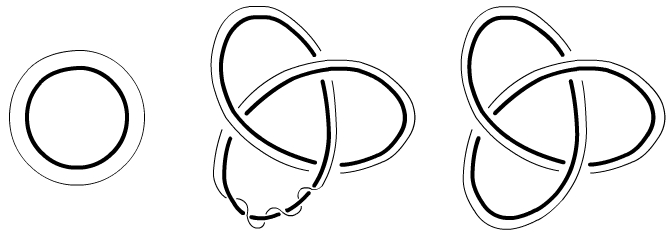
\includegraphics[scale=.5]{graphics/canonical-longitude}
\caption{Examples of the canonical longitude and a non-canonical longitude}
\label{canonical longitude}
\end{figure}

In \cref{canonical longitude} we have three knots drawn (the bolded knots) with longitudes (not bolded). The first two longitudes are canonical, as one can easily calculate their linking numbers to be 0. However the third longitude, which seems like a more obvious choice for a longitude than the second, is \emph{not} canonical since its linking number is -3.

The fundamental group of the knot complement $\pi_1(S^3 \backslash k)$ is called the \textbf{knot group}, and clearly is an invariant of the knot. There is a simple algorithm for computing a presentation of $\pi_1(S^3 \backslash k)$ given a diagram of $D$. For a diagram $D$ of $k$, let $n+1$ be the number of crossings. Let $\alpha_0,\ldots,\alpha_n$ be the arcs in $D$ that start at a crossing, travel along the under-strand, and end at the next crossing that the strand goes under such that $\alpha_i$ starts at where $\alpha_{i-1}$ ends (we always take the subscripts of the $\alpha$'s to be mod $n$). Also orient these arcs such that $\alpha_i$ points towards the starting point of $\alpha_{i+1}$. For convenience, suppose that $k$ does not pass through $(0,0,1)$ (the point at infinity in $\mathbb R^3$), and let us use this as the base point in $S^3 \backslash k$. In terms of the knot diagram, we can think of the base point as sitting right where we (the viewers) are, and so loops based at $\infty$ leave from us, travel through the knot diagram, and then return to us. Hence, a loop in the knot diagram can be represented by just a curve segment (\emph{not} a loop), and we just assume the ends are connected to the point at infinity in the obvious way.

Generators of $\pi_1(S^3 \backslash k)$ are just short arc segments $x_0,\ldots,x_n$ in the diagram such that $x_i$ passes under $\alpha_i$, and oriented so that it crosses under $\alpha_i$ from the right to the left. Each crossing of the knot diagram gives a relation $r_i$ on the generators of the fundamental group. Suppose the crossing is where the arcs $\alpha_i,\alpha_j$ and $\alpha_{j+1}$ come together for some indices $i$ and $j$ (hence $\alpha_i$ is the over-strand). If the sign of the crossing is $+1$, then we add the relation $x_i x_j = x_{j+1} x_i$, and if the sign is $-1$, then we add the relation $x_j x_i = x_i x_{j+1}$. Note that we are computing the sign of these crossings with the orientation on $k$ induced by the orientations on the $\alpha$ arcs, which were chosen for convenience. If we changed those orientations we would get an equivalent presentation of the fundamental group. Let $r_i$ denote the relation obtained at the crossing where $\alpha_i$ and $\alpha_{i+1}$ meet.
\begin{prop}
The fundamental group of $S^3 \backslash k$ is isomorphic to $\< x_0,\ldots,x_n \st r_0,\ldots,r_n \>$.
\end{prop}
\begin{proof}
First we isotope $k$ so that it lies in $\lcb z = 0 \rcb \subset \mathbb R^3$, except at a crossing where the understand dips to the $\lcb z=-\epsilon \rcb$ plane for a short segment, which we call $\beta_i$ for the crossing corresponding to where $\alpha_i$ and $\alpha_{i+1}$ meet. We will decompose $S^3 \backslash k$ into a bunch of pieces and apply van Kampen's theorem. Let $A = \lcb z \geq -\epsilon \rcb \backslash k$, and let $B_i$ ($i=0,\ldots,n$) be a small open rectangular box around the segment $\beta_i$, but with $\beta_i$ remove and with a thin tube connected the box to $\infty$. Finally, let $C$ be the complement of the closure of $A \cup B_0 \cup \cdots \cup B_n$. 

First we claim that $\pi_1(A)$ is a free group generated by $x_0,\ldots,x_n$. To see this let $\overline{\alpha}_i$ be the arc $\alpha_i$ whose endpoints dive straight down to connect to the plane $\lcb z=-\epsilon \rcb$, and let $\overline{k}$ be the union of these arcs. Then $\pi_1(S^3\backslash k)$ is isomorphic to $\pi_1(S^3 \backslash \overline{k})$, so we compute the later group. If we take a curtain below the arc $\overline{\alpha}_i$ to the plane $\lcb z=-\epsilon \rcb$ and then thicken it we get a ball $B_i$. Removing the $B_i$'s from $\lcb z \geq -\epsilon \rcb$ yields a simply connected space, so we determine what happens to the fundamental group when we add the pieces $B_i \backslash \overline{\alpha}_i$ back. The piece $B_i \backslash \overline{\alpha}_i$ is just a punctured disc, so its fundamental group is generated by a loop going around this hole once. Also the piece $B_i \backslash \overline{\alpha}_i$ intersects the space where we removed all the $B_j$'s from $\lcb z \geq -\epsilon \rcb$ is just a disc, hence we added one generator by adding the piece $B_i \backslash \overline{\alpha}_i$. Continuing this we get the claim.



\unfinished
\end{proof}
This presentation of the knot group is called the \textbf{Wirtinger presentation}.

\begin{example}
Consider the diagram of the trefoil knot $k$ shown in \cref{knot-group-trefoil} (we label our arcs by $A,B,C$ and generators of $\pi_1$ by $a,b,c$). The Wirtinger representation of the knot group is
\[ \pi_1(S^3 \backslash k) = \< a,b,c \st ba=ac, ac=cb, cb=ba \> \]
We can eliminate a generator from this presentation by seeing that $c = bab^{-1}$, hence another presentation of the fundamental group is given by
\[ \pi_1(S^3 \backslash k) = \< a,b \st bab=aba \> \]
If we set $x = aba$ and $y=ba$, then we see that $x^2 = abaaba = bababa = y^3$, hence yet another presentation is given by
\[ \pi_1(S^3 \backslash k) = \< x,y \st x^2 = y^3 \> \]

\begin{figure}[tb]
\centering
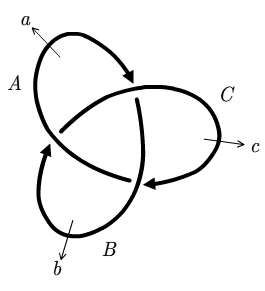
\includegraphics[scale=.5]{graphics/knot-group-trefoil}
\caption{Computing the knot group of the trefoil}
\label{knot-group-trefoil}
\end{figure}
\end{example}


\begin{example}
Let us compute the knot group of the $(p,q)$ torus knot $T_{p,q}$ (with $p,q \geq 1$ relatively prime). Arrange the knot to be on the boundary of the standardly embedded, unknotted solid torus $H$ in $S^3$. Then we can write $S^3 \backslash T_{p,q}$ as a union of $H \backslash T_{p,q}$ and $\overline{H^c} \backslash T_{p,q}$, each of which is clearly homotopy equivalent to a solid torus. The intersection of these sets is an annulus, and the fundamental group of each is freely generated by loops $x$ and $y$. By the Seifert-van Kampen theorem we have $\pi_1(S^3 \backslash T_{p,q})$ is generated by $x$ and $y$ with the relation $x^p = y^q$, hence
\[ \pi_1(S^3 \backslash T_{p,q}) = \< x,y \st x^p = y^q \> \]
\end{example}



\subsection{The Alexander Polynomial}
\label{The Alexander Polynomial}



We will now construct some classical invariants of knots and links in $S^3$. With some work these invariants can be extended to links in integral homology spheres, as we will see later. These combinatorial invariants have very interesting relationships with ``high-powered'' invariants, like Seiberg-Witten invariants and Heegaard Floer homology.

Fix a diagram $D$ of a knot $L$ in $S^3$ with $n$ components, and give the link any orientation. Suppose this diagram has $k$ double points and the oriented resolution of this diagram has $c$ connected components. Let us compute the Euler characteristic and genus of the Seifert surface $F$ constructed from Seifert's algorithm on $D$ (see \cref{Seifert's algorithm}). The Euler characteristic of $c$ disjoint discs is $c$, and attaching a band to these discs decreases the Euler characteristic by one. Therefore $\chi(F) = c - k$. On the other hand, an orientable surface of genus $g$ with $n$ boundary components has Euler characteristic $2-2g-n$. Setting these two Euler characteristics equal to each other and solving for $g$ shows that the genus of $F$ is 
\begin{equation}
\label{genus of surface from Seifert's algorithm}
g = 1 + \frac{k-c-n}{2}
\end{equation}
One can compute that the first homology of a surface of genus $g$ with $n \geq 1$ boundary components is the free abelian group of rank $2g+n-1$ (just look at the handlebody decomposition of such a surface), therefore, by \eqref{genus of surface from Seifert's algorithm}, $H_1(F)$ is free abelian with rank $1+k-c$. 

Now, for a general Seifert surface $F$ of a link $L$ in $S^3$, let $\alpha=(x_1,\ldots,x_\ell)$ be an ordered collection of non-intersecting, oriented, closed curves in $F$ that form an ordered basis for $H_1(F)$. Choose an orientation of $F$ by specifying a nowhere zero, normal vector field $n$ on $F$. For each curve $x_i$, let $x_i^+$ be the curve in $S^3$ that is $x_i$ pushed off the surface $F$ slightly in the direction of $n$. For each pair of curves $x_i,x_j^+$ we can compute their linking numbers (they do not intersect), and so we define the \textbf{Seifert matrix} of $F$ with orientation $n$ to be the matrix $[F] = (\lk(x_i,x_j^+))_{i,j=1}^\ell$. Of course this matrix depends on our choice of orientation of $F$ and basis for $H_1(F)$, so to include this dependence in the notation we may sometimes write $[F]_{\alpha,n}$. Suppose we have fixed our basis $x_1,\ldots,x_\ell$ with pushed off curves $x_1^+,\ldots,x_\ell^+$ relative to $n$. If we change the orientation of $F$ to $-n$, then we can translate $F$ a little bit so that $x_1^+,\ldots,x_\ell^+$ lie in $F$, in which case the curves $x_1,\ldots,x_\ell$ are now the pushed off curves relative to $-n$. So, the Seifert matrix with respect to this orientation is $(\lk(x_i^+,x_j))$. This is equal to $(\lk(x_j,x_i^+))$ by the symmetry of linking numbers, which is the transpose of the Seifert matrix computed with respect to $n$. So, reversing orientations transposed the Seifert matrix. If we fix the orientation, then any two bases of $H_1(F)$ are related by an invertible matrix $U$ (invertible over $\mathbb Z$ means $\det U=\pm 1$), so if $\alpha$ and $\beta$ are two bases related by $U$, then $[F]_\beta = U^T [F]_\alpha U$.

However, even if we consider two Seifert matrices $A$ and $B$ equivalent if they are related by $A=U^TBU$, for some invertible $U$, we do not get a knot invariant. We could just analyze how Seifert matrices transform under the Reidemeister moves, but a nicer way is to find a set of moves that can be performed on Seifert surfaces such that any two Seifert surfaces of a knot are related by these moves. On such move is \textbf{ambient isotopy}; that is, if $G : S^3 \times I \rightarrow S^3$ is an isotopy of $S^3$ and $F$ is a Seifert surface for a knot $k$, then we say $F' = G(F,1)$ is an ambiently isotopic Seifert surface of the isotopic knot $k' = G(k,1)$. Another move is to remove two disjoint discs $D_1,D_2$ in the interior of $F$, and glue in an embedded tube $S^1 \times I$ that is disjoint from the rest of $F$. This increases the genus of $F$ by one, but does not change the boundary. This move is called \textbf{stabilization}. The inverse of this move, called \textbf{destabilization}, is the process of finding a curve $c$ on $F$ such that $c$ bounds a disc in $S^3 \backslash F$, cutting $F$ open along $c$, and then closing $F$ back up by gluing two discs in. This move decreases the genus of $F$ by one.
\begin{prop}
\label{stabilization of Seifert surfaces}
Any two Seifert surfaces $F,F'$ of isotopic knots $k,k'$ can be connected via a finite sequence of ambient isotopies, stabilizations and destabilizations.
\end{prop}
\begin{proof}[Sketch]
Let $G : S^3 \times I \rightarrow S^3$ be an ambient isotopy between $k$ and $k'$, i.e. $G(k,1) = k'$. The set $M'$ of points $(G(x,t),t) \in S^3 \times I$, as $(x,t)$ ranges of $k \times I$, is an embedded surface in $S^3 \times I$. We can close this surface up by setting $M = (F \times 0) \cup M' \cup (F \times 1)$ to get an embedded, closed surface in $S^3$, and it bounds a 3-manifold $W$ ($\partial W = M$). Slightly perturbing $M$ and $W$, if necessary, we have that the time slices $S^3 \times t \cap W$ are smoothly embedded surfaces in $S^3$ with boundary $G(k,t)$, except possibly at finitely many points. From standard Morse theory that crossing these critical points changes $S^3 \times t \cap W$ by a surgery, depending on the index of the critical point. We can arrange that there are only critical points of index 1 and 2, which correspond to destabilization and stabilization respectively. 
\end{proof}

We have already remarked that a change of basis of $H_1(F)$ corresponds to changing the Seifert matrix of $F$ by $U^TSU$, for some integral matrix with $\det U = \pm 1$. Let us see how stabilization of a Seifert surface changes the Seifert matrix. Let $F$ be a Seifert surface of $k$ with generators $x_1,\ldots,x_{2g}$ for $H_1(F)$. By forming $F' = F \sharp T'$ we are adding two generators to the first homology, one curve going around the longitude of $T'$ and one curve going around the meridian, so let $y$ and $z$ denote these curves. Since the torus $T'$ can knot and link with $F$ in complicated ways, we have that column and row of $[F']$ corresponding to $y$ can consist of arbitrary integers, except that either $\lk(y,z^+)=\pm 1$ and $\lk(z,y^+)=0$, or the opposite. Therefore the Seifert matrix $[F']$ is given by
\[ \begin{pmatrix}  & & & * & 0 \\ & [F] & & \vdots & \vdots \\ & & & * & 0 \\ * & \cdots & * & * & \pm 1 \\ 0 & \cdots & 0 & 0& 0 \end{pmatrix}  \text{\ \ \ \ \ or \ \ \ \ \ } \begin{pmatrix}  & & & * & 0 \\ & [F] & & \vdots & \vdots \\ & & & * & 0 \\ * & \cdots & * & * & 0 \\ 0 & \cdots & 0 & \pm 1 & 0 \end{pmatrix} \]

This leads us to define two operations we can perform on integral matrices. Given an integral, $n \times n$ matrix $A$ (not necessarily invertible), performing an $S_1$ move is to change the matrix to $U^TAU$ for some invertible integral matrix $U$. Performing an $S_2$ move is to change the matrix to the $(n+2) \times (n+2)$ matrix given by
\begin{equation}
\label{S_2 move}
\begin{pmatrix}  & & & * & 0 \\ & S & & \vdots & \vdots \\ & & & * & 0 \\ * & \cdots & * & * & \pm 1 \\ 0 & \cdots & 0 & 0& 0 \end{pmatrix}
\end{equation}
where the $*$'s can be any numbers. We say that two integral matrices are \textbf{$S$-related} one can be brought to the other with a finite sequence of $S_1$ and $S_2$ moves. An immediate consequence of \cref{stabilization of Seifert surfaces} is
\begin{cor}
\label{Seifert matrices are S-equivalent}
Any two Seifert matrices of a knot are $S$-equivalent.
\end{cor}

Therefore the $S$-equivalence class of any Seifert matrix of a knot is an invariant of the knot. There are simpler or more computable invariants we can derive from the Seifert matrix. Given a knot $k$, let $S$ be any Seifert matrix for $k$. The Laurent polynomial 
\[ \Delta_k(t) = \det \left( t^{1/2} S - t^{-1/2} S^T \right) \]
in $t^{1/2}$ is called the \textbf{Alexander polynomial} of $k$. Technically we should call this the Conway normalization of Alexander's polynomial, as Alexander's original definition used the infinite cyclic covering of the knot complement, and was defined only up to multiplication by a unit. Since the dimension of $S$ is $2g$ (where $g$ is the genus of the surface associated to $S$) we have $\Delta_k(t)$ is actually a Laurent polynomial in $t$, and a direct substitution shows $\Delta_k(t)=\Delta_k(t^{-1})$. If $S$ is of genus $g$, then we can easily see that $\Delta_k(t) = t^{-g}\det(S-tS^T)$.

\begin{prop}
\label{Alexander polynomial is a knot invariant}
The Alexander polynomial does not depend on the Seifert matrix chosen, hence is a knot invariant.
\end{prop}
\begin{proof}
If $S'$ is another Seifert matrix for $k$, then $S$ and $S'$ are related by a finite sequence of $S_1$ and $S_2$ moves by \cref{Seifert matrices are S-equivalent}. Let $\Delta_k(t)$ denote the Alexander polynomial with respect to $S$, and $\Delta_k'(t)$ the Alexander polynomial with respect to $S'$. If $S' = U^TSU$, then we see that
\begin{align*}
	\Delta_k'(t) &= \det \left( t^{1/2} U^TSU - t^{-1/2} U^TSU \right) \\
	             &= (\det U)^2 \det \left( t^{1/2} S - t^{-1/2} S^T \right) \\
	             &= \Delta_k(t)
\end{align*}
where the last line follows since $\det U = \pm 1$. On the other hand, if $S'$ is the result of performing the $S_2$ move on $S$ (see \eqref{S_2 move}), then $S'^T$ can be written as
\[ \begin{pmatrix}  & & & * & 0 \\ & S^T & & \vdots & \vdots \\ & & & * & 0 \\ * & \cdots & * & * & 0 \\ 0 & \cdots & 0 & 1 & 0 \end{pmatrix} \]
and the matrix $t^{1/2} S' - t^{-1/2} S'^T$ can be written as
\[ \begin{pmatrix}  & & & * & 0 \\ & t^{1/2} S - t^{-1/2} S^T & & \vdots & \vdots \\ & & & * & 0 \\ * & \cdots & * & * & t^{1/2} \\ 0 & \cdots & 0 & -t^{-1/2} & 0 \end{pmatrix} \]
When computing the determinant of this matrix we can perform a cofactor expansion along the last column, and then another cofactor expansion along the last row of the resulting matrix, in which case we see that the determinant of the above is precisely
\[ -t^{-1/2} \left( -t^{1/2} \det \left( t^{1/2} S - t^{-1/2} S^T \right) \right) = \Delta_k(t) \]
hence the Alexander polynomial is invariant under the $S_2$ moves. 
\end{proof}

We can extend the definition of Alexander polynomial to links in the obvious way, but it will no longer be independent of the Seifert surface. The problem is that a link $L$ with $n$ components has $2^n$ orientations. A Seifert surface $F$ for $L$ can induce two of these orientations on $L$ (and they are opposite), and conversely we say that a Seifert surface is compatible with an oriented link if the induced orientation agrees with the link's orientation. While it is true that any two Seifert surfaces compatible with an oriented link are stably equivalent, it is \emph{not} true that any two Seifert surfaces of a link are stably equivalent. So, the Alexander polynomial is an invariant of oriented links with compatible Seifert matrices.

As mentioned above, the Alexander polynomial is not sensitive to the orientation of a knot, i.e. $\Delta_k(t) = \Delta_{-k}(t)$. Unfortunately, the Alexander polynomial is also not sensitive to changing a knot to its mirror. The \textbf{mirror} of a knot $k$ is the knot $\overline{k}$ obtained by reflecting $k$ through any plane in $\mathbb R^3$. This is equivalent to changing all over crossings to under crossings (and vice versa) in a diagram of $k$.
\begin{prop}
For any knot $k$, $\Delta_{k}(t) = \Delta_{\overline{k}}(t)$.
\end{prop}
\begin{proof}
If $S$ is a Seifert matrix of $k$, then $-S$ is a Seifert matrix of $\overline k$. Let $2m$ be the order of $S$. Then
\begin{align*}
\Delta_{\overline k}(t) &= \det\left( -t^{1/2} S + t^{-1/2} S^T \right) \\
                        &= \det\left( t^{-1/2} S^T - t^{1/2} S \right) \\
                        &= \det\left( t^{-1/2} S - t^{1/2} S^T \right) \\
                        &= \Delta_k(t^{-1}) = \Delta_k(t) 
\end{align*}
\end{proof}

There are also scalar invariants of knots that one can derive from Seifert matrices.

\begin{prop}
\label{knot determinant}
If $S$ is the Seifert matrix of some Seifert surface of a knot $k$, then $|\det(S+S^T)|$ is a knot invariant.
\end{prop}
\begin{proof}
We just have to check that $|\det(S+S^T)|$ does not change after applying $S_1$ and $S_2$ moves to $S$. If we change $S$ by $U^TSU$, then clearly 
\[ |\det(U^TSU + U^TS^TU)| = |(\det U)^2 \det(S+S^T)| = |\det(S+S^T)| \]
Let $S'$ be the matrix resulting from applying $S_1$ to $S$ (see \eqref{S_2 move}). Then $S'+S'^T$ is of the form
\[ \begin{pmatrix}  & & & * & 0 \\ & S + S^T & & \vdots & \vdots \\ & & & * & 0 \\ * & \cdots & * & * & \pm 1 \\ 0 & \cdots & 0 & \pm 1 & 0 \end{pmatrix} \]
By adding multiples of the last column to the other columns, and multiples of the last row to the other rows we can bring this matrix into the form
\begin{equation}
\label{elementary transformations on S+S^T}
\begin{pmatrix}  & & & 0 & 0 \\ & S + S^T & & \vdots & \vdots \\ & & & 0 & 0 \\ 0 & \cdots & 0 & 0 & \pm 1 \\ 0 & \cdots & 0 & \pm 1 & 0 \end{pmatrix}
\end{equation}
and the determinant of this matrix is $-\det(S+S^T)$. Therefore the absolute value of this determinant remains invariant under $S_1$ and $S_2$ moves.
\end{proof}

We call $|\det(S+S^T)|$ the \textbf{determinant} of the knot $k$, and denote it by $\det(k)$. The relationship between the determinant of $k$ and the Alexander polynomial is clear.
\begin{prop}
$|\Delta_k(-1)| = \det(k)$
\end{prop}
\begin{proof}
Let $S$ be any Seifert matrix of $k$ and let $2m$ be the order of $S$ (the order must be even for a knot). Then
\begin{align*}
|\Delta_k(-1)| &= \left| \det\left( (-1)^{1/2} S - (-1)^{-1/2} S^T \right) \right| \\
               &= \left| \det\left( (-1)^{1/2} S + (-1)^{1/2} S^T \right) \right| \\
               &= \left| (-1)^m \det(S+S^T) \right|
\end{align*}
\end{proof}

The Alexander polynomial satisfies a skein relation, which is closely related to another polynomial invariant that is essentially the same as the Alexander polynomial. For an oriented link $L$ and a diagram $D$ of $L$, choose any crossing in this diagram and let $L_+$ denote the diagram resulting from switching this crossing to a positive crossing, $L_-$ the diagram resulting from switching to a negative crossing, and $L_0$ the diagram resulting from resolving the crossing in the oriented way (see \cref{??}). 
\begin{thm}
The Alexander polynomial of an oriented link $L$ satisfies the skein relation
\[ \Delta_{L_+}(t) - \Delta_{L_-}(t) = (t^{1/2}-t^{-1/2}) \Delta_{L_0}(t) \]
Further, this relation, along with the normalization $\Delta_\text{unknot}(t)=1$, uniquely determines the Alexander polynomial as a function from oriented links to $\mathbb Z[t^{1/2},t^{-1/2}]$.
\end{thm}
\begin{proof}
Let $F_0$ be the Seifert surface for $L_0$ constructed from Seifert's algorithm (see \cref{Seifert's algorithm}). We can construct Seifert surfaces $F_\pm$ for $L_\pm$ by gluing in a twisted band. Take a basis $\lcb x_1,\ldots,x_{k-1} \rcb$ for $H_1(F_0)$, then we can get a basis for $H_1(F_\pm)$ by adding one extra curve $x_k$ that goes through the twisted band once. Let $S_0$ be the Seifert matrix of $F_0$ computed with respect to $\lcb x_1,\ldots,x_{k-1} \rcb$. The Seifert matrices $S_\pm$ of $F_\pm$ are of the form
\[ S_+ = \begin{pmatrix} 
			    &        &         & b_1 \\
			    & S_0    &         & \vdots \\
			    &        &         & b_{k-1} \\
			a_1 & \cdots & a_{k-1} & N
		  \end{pmatrix}
\ \ \ \ \ \ \ 
   S_- = \begin{pmatrix} 
			    &        &         & b_1 \\
			    & S_0    &         & \vdots \\
			    &        &         & b_{k-1} \\
			a_1 & \cdots & a_{k-1} & N-1
		  \end{pmatrix}
\]
for some integers $a_1,\ldots,a_k,b_1,\ldots,b_k,N$. Writing out the entries of $t^{1/2}S_\pm - t^{-1/2}S_\pm^T$ we see that the last column and row of these matrices are equal, except for the bottom-right corner entry where one matrix has $(t^{1/2}-t^{-1/2})N$ and the other has $(t^{1/2}-t^{-1/2})(N-1)$. So, if we compute $\Delta_{L_+}(t) - \Delta_{L_-}(t)$ by performing a cofactor expansion along the last columns, then the terms from $\Delta_{L_+}(t)$ will cancel those from $\Delta_{L_-}(t)$ except for the last term, which is equal to
\[ (-1)^{2k} (t^{1/2}-t^{-1/2})N \Delta_{L_0}(t) - (-1)^{2k} (t^{1/2}-t^{-1/2})(N-1) \Delta_{L_0}(t) = (t^{1/2}-t^{-1/2}) \Delta_{L_0}(t)   \]
Therefore $\Delta_L(t)$ satisfies the skein relation. 
\end{proof}

Although the Alexander polynomial satisfies a skein relation, this relation does not quite look like the relation for the Jones polynomial. To make things more uniform we introduce the Conway polynomial $\nabla_L(z)$. This is a function $\nabla : \lcb \text{oriented links} \rcb \rightarrow \mathbb Z[z]$ that is uniquely determined by the normalization $\nabla_{\text{unknot}}(z) = 1$ and the skein relation
\[ \nabla_{L_+}(z) - \nabla_{L_-}(z) = z \nabla_{L_0}(z) \]
The relationship between the Alexander and Conway polynomial is given by $\Delta_L(t) = \nabla_L\left( t^{1/2}-t^{-1/2} \right)$.



\subsection{Knot Signatures and 4-Ball Genus}
\label{Knot Signatures and 4-Ball Genus}

A very important invariant of knots is the signature. 

\begin{prop}
\label{knot signature}
Let $\omega$ be a unit complex number not equal to 1, and let $S$ be a Seifert matrix of the knot $k$. Then the signature of the Hermitian matrix $(1-\omega)S + (1-\overline\omega)S^T$ over $\mathbb C$ is an invariant of the knot.
\end{prop}
\begin{proof}
We just have to check that the signature of $(1-\omega)S+(1-\overline\omega)S^T$ does not change after applying $S_1$ and $S_2$ moves to $S$. Clearly the signature is invariant under $S_1$ moves. Let $S'$ be the Seifert matrix resulting in applying an $S_2$ move, then we have $(1-\omega)S+(1-\overline\omega)S^T$ is congruent to
\[ \begin{pmatrix}  & & & 0 & 0 \\ & (1-\omega)S + (1-\overline\omega)S^T & & \vdots & \vdots \\ & & & 0 & 0 \\ 0 & \cdots & 0 & 0 & 1-\omega \\ 0 & \cdots & 0 & 1-\overline\omega & 0 \end{pmatrix} \]
The signature of this block matrix is the sum of the signatures of the blocks. Since the signature of the bottom-right block is zero, we have that the signature of the above matrix is the signature of $(1-\omega)S+(1-\overline\omega)S^T$, hence the signature is invariant under $S_2$ moves.
\end{proof}
We call the signature of $(1-\omega)S+(1-\overline\omega)S^T$ the \textbf{$\omega$-signature} of the knot, and denote it by $\sigma_\omega(k)$. If $\omega=-1$, then we just call this \emph{the} signature of $k$, and denote it by $\sigma(k)$.

For a knot $k$ in $S^3$, consider the 4-ball $D^4$ bounded by $S^3$. Let $g^*(k)$ denote the minimal genus of a surface $F$ that can be smooth embedded in $D^4$ with $\partial F = k \subset S^3$. This knot invariant is called the \textbf{smooth 4-ball genus}, or sometimes the \textbf{smooth slice genus}. A knot is said to be \textbf{slice} if $g^*(k)=0$. The relationship between signature and slice knots is the following.
\begin{thm}
\label{slice knots and signature}
If $k$ is a slice knot, then $\sigma(k)=0$.
\end{thm}

We will outline the proof of this theorem in a series of lemmas. Suppose $k$ is a slice knot with slicing disc $D \subset D^4$. If $F$ is a Seifert surface for $k$ in $S^3$, then we can glue together $F \cup D$ to obtain a closed surface in $D^4$.
\begin{lem}
The surface $F \cup D$ bounds a smoothly embedded, orientable 3-manifold $M$ in $D^4$ with $M \cap S^3 = F$.
\end{lem}

\begin{lem}
Let $M$ be a compact, orientable 3-manifold such that $\partial M$ is a surface of genus $g$. Then the kernel of the map $i_* : H_1(\partial M;\mathbb Q)\rightarrow H_1(M;\mathbb Q)$ induced by the inclusion is of dimension $g$.
\end{lem}
\begin{proof}
We can put the homology and cohomology long exact sequences of the pair $(M,\partial M)$ into the following commutative diagram
\[
\xymatrix
{
	H_2(M,\partial M;\mathbb Q) \ar[r] \ar[d] & H_1(\partial M;\mathbb Q) \ar[r]^{i_*} \ar[d] & H_1(M;\mathbb Q) \ar[d] \\
	H^1(M;\mathbb Q) \ar[r]^{i^*} & H^1(\partial M;\mathbb Q) \ar[r]^{\delta} & H^2(M,\partial M;\mathbb Q)
}
\]
where the vertical arrows are the Poincar\'{e} and Poincar\'{e}-Lefschetz duality isomorphisms. By the universal coefficient theorem we have that $H^1(\partial M;\mathbb Q)$ is dual to $H_1(\partial M;\mathbb Q)$, $H_1(M;\mathbb Q)$ is dual to $H^1(M;\mathbb Q)$, and $i^*$ is dual to $i_*$. By the rank-nullity theorem we have 
\[ 2g = \dim \image i_* + \dim \ker i_* = \dim \image i_* + \dim \ker \delta = \dim \image i_* + \dim \image i^* = 2 \dim \image i_* \]
hence $\dim \image i_* = g$, and so $\dim \ker i_* = g$.
\end{proof}

\begin{lem}
There is a basis $\lcb x_i \rcb$ over $\mathbb Z$ for $H_1(\partial M;\mathbb Z)$ such that $i_*(x_j)=0$ in $H_1(M;\mathbb Q)$ for $1 \leq j \leq g$.
\end{lem}
\begin{proof}
We think of $H_1(\partial M) = \mathbb Z^{2g}$ as sitting inside $H_1(\partial M;\mathbb Q) = \mathbb Q^{2g}$. Let $U$ be the $g$ dimensional subspace of $\mathbb Q^{2g}$ which is the kernel of the map $\mathbb Q^{2g} \rightarrow H_1(M;\mathbb Q)$ induced by the inclusion. We can take a basis $\lcb x_1,\ldots,x_g \rcb$ for this vector space such that $x_i \in \mathbb Z^{2g}$, and so let $\widetilde{U}$ be the $\mathbb Z$-span of these vectors. 

As a $\mathbb Z$-module we can write $\mathbb Z^{2g} / \widetilde U$ as $A / \widetilde U \oplus B / \widetilde U$, where $A$ and $B$ are submodules of $\mathbb Z^{2g}$ such that $A / \widetilde U$ is free and $B / \widetilde U$ is torsion. The fact that this latter module is torsion means that for $b \in B$ there is an integer $n$ such that $nb \in \widetilde U$, hence $nb \in U$, or simply $b \in U$. Thus a $\mathbb Z$-basis for $B$ also serves as a $\mathbb Q$-basis for $U$. So, the $\mathbb Z$-basis we take for $H_1(\partial M)$ is any extension of a basis for $B$ to a full basis for $H_1(\partial M)$. 
\end{proof}

\begin{lem}
Let $F$ be a genus $g$ Seifert surface for a slice knot $k$. Then there is a basis for $H_1(F)$ such that the associated Seifert matrix is of the form
\[ S = \begin{pmatrix} 0 & P \\ Q & R \end{pmatrix} \]
for some $g \times g$ matrices $P,Q,R$.
\end{lem}
\begin{proof}
Let $D$ be a slicing disc for $k$ in $D^4$ so that there is a 3-manifold $M$ with $\partial M = F \cup D$. Let $\lcb x_i \rcb$ be a $\mathbb Z$-basis for $H_1(\partial M)$ as in the previous lemma so that $x_i=0$ in $H_1(M;\mathbb Q)$ for $1 \leq i \leq g$. We can assume that the homology classes $x_i$ are represented by oriented, closed curves in $\partial M$, and we will also write $x_i$ to denote these curves. For each $1 \leq i \leq g$ we can find a non-zero integer $n_i$ such that $n_i x_i = 0$ in $H_1(M)$. The class $n_i x_i$ can be represented by a closed curve in $\partial M$, which we also denote by $n_i x_i$, and it bounds a 2-chain in $M$. This means we can find maps $f_i : F_i \rightarrow D^4$, where $F_i$ is a surface with boundary, such that $f_i(\partial F_i) = n_i x_i$. If we push the curve $n_i x_i$ off of $\partial M$ in the normal direction, then we can also pushing the mapping $f_i$ in this direction. Therefore, for $1 \leq i,j, \leq g$ the curves $n_i f_i$ and $(n_j f_j)^+$ bound disjoint surfaces in $D^4$, and hence 
\[ 0 = \lk(n_if_i,(n_jf_j)^+) = n_in_j \lk(f_i,f_j^+) \]
Therefore the upper-left $g \times g$ block of the Seifert matrix of $F$ with respect to the basis $\lcb x_i \rcb$ is zero.
\end{proof}

\begin{lem}
If $B$ is a symmetric, non-degenerate bilinear form on an even dimensional space such that there is a half dimensional space $U$ with $B(u,u')=0$ for all $u,u' \in U$, then $B$ has zero signature.
\end{lem}
\begin{proof}
Suppose the space $V$ that $B$ is defined on is of dimension $2g$, and let $U$ be a subspace of dimension $g$ where $B$ vanishes. If $V^\pm$ denote the maximal positive/negative-definite subspaces of $V$ with respect to $B$, then $V = V^+ \oplus V^-$ since $B$ is non-degenerate. However, we also have $U \cap V^+ = \lcb 0 \rcb$ and $U \cap V^- = \lcb 0 \rcb$, hence $\dim V^+ \leq g$ and $\dim V^- \leq g$. Since we need $\dim V^+ + \dim V^- = 2g$ we are forced to have $g = \dim V^+ = \dim V^-$, which implies $\sigma(B)=0$.
\end{proof}


\begin{proof}[Proof of \Cref{slice knots and signature}]
Clearly the combination of the previous lemmas proves the theorem.
\end{proof}

More generally one can also prove
\begin{thm}
\label{signature 4-ball genus bound}
For any knot $k$ we have $|\sigma(k)| \leq 2g^*(k)$.
\end{thm}

For a knot $k$, let $u(k)$ denote the minimum number of crossing changes needed in a diagram of $k$ in order to obtain the unknot. This number is called the \textbf{unknotting number} of $k$. We can think of the process of unknotting $k$ as a movie in $S^3 \times [0,1]$ (i.e. an embedded surface), such that the $t$ slice of the surface is an embedded knot in $S^3 \times \lcb t \rcb$ for all but finitely many values of $t$. At one of these singular times $t$ we can find $\epsilon > 0$ small enough so that the $t \pm \epsilon$ slices of the surface are embedded knots, and differ only by a crossing change. Further, if there are two times $t_0,t_1$ such that the slices of the surface at all times between $t_0,t_1$ are embeddings, then the slice at $t_0$ and $t_1$ differ only by Reidemeister moves. 

Now, let $\Sigma \subset S^3 \times [0,1]$ be an embedded surface such that $\Sigma \cap S^3 \times \lcb 0 \rcb = k$ and $\Sigma \cap S^3 \times \lcb 1 \rcb$ is the unknot, and let $\Sigma_t = \Sigma \cap S^3 \times \lcb t \rcb$ and $\Sigma_{\leq t} = \Sigma \cap S^3 \times [0,t]$. If $\Sigma_t$ is singular, then we claim that the genus of $\Sigma_{\leq t+\epsilon}$ is strictly greater than $\Sigma_{\leq t-\epsilon}$. \unfinished .... We have proved the following.
\begin{lem}
$g^*(k) \leq u(k)$
\end{lem}
\begin{cor}
$|\sigma(k)| \leq 2g^*(k) \leq 2u(k)$
\end{cor}

We say that two knots $k_1,k_2$ in $S^3$ are \textbf{concordant} if there is a smooth embedding of a cylinder $S^1 \times I$ in $S^3 \times I$ such that $S^1 \times \lcb i \rcb$ maps to $k_i \times \lcb i \rcb$ ($i=0,1$). Concordance defines an equivalence relation on the set of knots in $S^3$. If a knot $k$ is concordant to the unknot, then we can cap off the unknot with a disc and obtain a smoothly embedded disc in $D^4$ that is bounded by $k$, hence $k$ is slice. Therefore a knot is concordant to the unknot if and only if it is slice.

Let $\mathcal C_1$ denote the concordance classes of knots in $S^3$. If $k_1,k_1'$ and $k_2,k_2'$ are concordant pairs of knots, then $k_1 \# k_2$ and $k_1' \# k_2$ are concordant. The cobordism can be constructed by splicing together the cylinders connected $k_1$ to $k_1'$ and $k_2$ to $k_2'$. Next we claim that for any knot $k$, the knot $k \# \overline k$ is slice. Define the following subsets of $\mathbb R^4$:
\[ \mathbb R^3 = \lcb (x,y,z,0) \in \mathbb R^4 \rcb \]
\[ \mathbb R_-^3 = \lcb (x,y,z,0) \in \mathbb R^4 \st z \leq 0 \rcb \]
\[ \mathbb R_+^3 = \lcb (x,y,z,0) \in \mathbb R^4 \st z \geq 0 \rcb \]
\[ \mathbb R^2 = \lcb (x,y,0,0) \in \mathbb R^4 \rcb \]
Arrange the knot $k \# \overline k$ in $\mathbb R^3$ so that its intersection with the plane $\mathbb R^2$ in $\mathbb R^4$ consists of two points on the band used in the connect sum. Let $k^+$ denote the intersection of $k \# \overline k$ with $\mathbb R_+^3$, which is just an arc, so that if $k_-$ is the reflection of $k_+$ through $\mathbb R^2$, then $k_+ \cup k_-$ is isotopic to $k \# \overline k$. Consider the set of points
\[ D = \lcb (x,y,z\cos\theta,z\sin\theta) \in \mathbb R^4 \st (x,y,z,0) \in k_+, 0 \leq \theta \leq \pi \rcb \]
That is, we spin all the points on $k_+$ about the plane $\mathbb R^2$ in $\mathbb R^4$ through all angles from $0$ to $\pi$. Clearly $D$ is just a disc (being a half spin of an arc) with boundary $k \# \overline k$, and this provides us with a slicing disc for $k \# \overline k$.

We can now conclude that $\mathcal C_1$ forms a group under connect sum with $[\text{unknot}]$ serving as the identity and the mirror of a knot serving as its inverse. Further, if $k_1$ and $k_2$ are concordant, then $0=\sigma(k_1 \# \overline k_2) = \sigma(k_1)-\sigma(k_2)$, hence $\sigma$ descends to a well-defined group homomorphism $\sigma : \mathcal C_1 \rightarrow \mathbb Z$.

A knot $k$ is said to be amphichiral if it is isotopic to its mirror $\overline k$. In particular, such a knot is an element of order 2 in $\mathcal C_1$. The figure-eight know is amphichiral, as shown in \cref{figure-eight-amphichiral}.

\begin{figure}[tb]
\centering
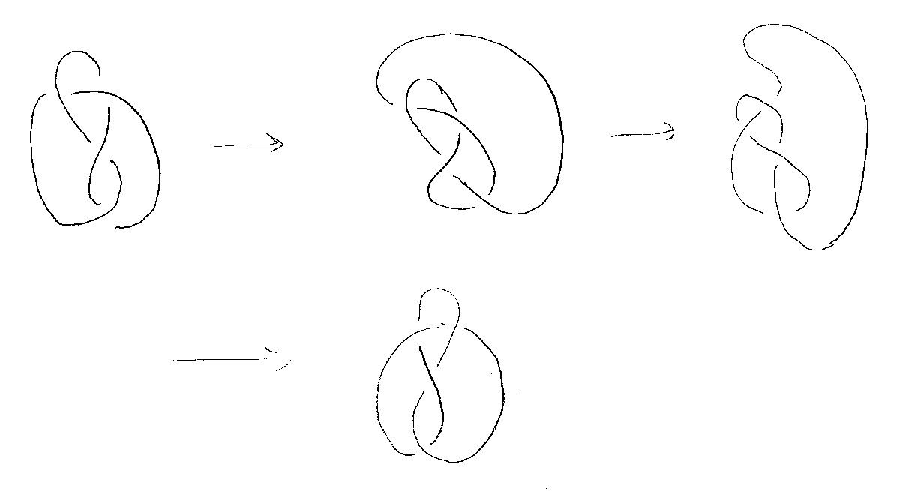
\includegraphics[scale=1]{graphics/figure-eight-amphichiral}
\caption{Showing the figure-eight knot is isotopic to its mirror}
\label{figure-eight-amphichiral}
\end{figure}





\subsection{Cyclic and Branched Covers}
\label{Cyclic and Branched Covers}


Now let us discuss Alexander's original definition of his polynomial using the infinite cyclic cover of the complement of a link. To construct this covering space we fix an oriented link $L$, set $X = S^3 \backslash L$, and fix a Seifert surface $F$ (compatible with the orientation of $L$). Let $Y$ be the space obtained from cutting $X$ along $F$ so that $\partial Y$ consists of two disjoint copies of $F$, denoted by $F_+$ and $F_-$; that is, $Y$ is homeomorphic to the complement of an open tubular neighborhood of $F$ in $S^3$. There is a natural identification $\phi : F_- \rightarrow F_+$. Take the countable collection $Y \times \lcb i \rcb$ ($i \in \mathbb Z$) of copies of $Y$, and let $h_i : Y \rightarrow Y_i$ be the obvious homeomorphism. Form the space $X_\infty$ by gluing $Y_i$ to $Y_{i+1}$ via the homeomorphism $h_{i+1} \circ \phi \circ h_i^{-1}$; that is, we glue $Y_i$ to $Y_{i+1}$ by gluing $F_- \times \lcb i \rcb$ to $F_+ \times \lcb i+1 \rcb$ via the map $h_{i+1} \circ \phi \circ h_i^{-1}$. The obvious projection $\pi : X_\infty \rightarrow X$, where $\pi|_{Y_i} : Y_i \rightarrow X$ is given by $\pi(x,i)=x$, is an infinite cyclic covering space of $X$.

Let $t$ denote the covering transformation of $X_\infty$ whose restriction $t|_{Y_i} : Y_i \rightarrow X_\infty$ is given by $t(x,i) = (x,i+1)$. This map induces an isomorphism (which we also denote by $t$) $t : H_1(X_\infty) \rightarrow H_1(X_\infty)$, turning $H_1(X_\infty)$ into a $\mathbb Z[t,t^{-1}]$-module, called the Alexander module of $L$. Of course, we need to show that this module is independent of the various choices in its construction

\begin{prop}
If $X_\infty$ and $X_\infty'$ are the infinite cyclic coverings of the link complement $X$ of a link $L$ constructed from two different Seifert surfaces, then $X_\infty$ and $X_\infty'$ are isomorphic has covering spaces, and $H_1(X_\infty)$ and $H_1(X_\infty')$ are isomorphic as $\mathbb Z[t,t^{-1}]$ modules.
\end{prop}
\begin{proof}
Recall that covering spaces are determined up to equivalence by the image of the fundamental group of the total space under the covering projection. That subgroup of the fundamental group of the base space consists of those loops in the base that lift to loops in the total space. So, we show that the notion of lifting loops to loops does not depend on the Seifert surface $F$ used in the construction of $X_\infty$.

Let $\alpha : [0,1] \rightarrow X$ be any path in $X$ and consider a lift $\tilde\alpha : [0,1] \rightarrow X_\infty$. This path is a loop in $X_\infty$ if and only if $\tilde\alpha(0)$ and $\tilde\alpha(1)$ are both in $X_\infty$, which means the path intersects the chambers $F_\pm \times \lcb i \rcb$ with algebraic multiplicity zero. Down in $X$ this means that that $\alpha$ has zero algebraic intersection number with $F$, which we know is equivalent to $\alpha$ and $L$ having zero linking number (which is the sum of the linking numbers with each component of $L$). This statement is of course independent of $F$, hence our notion of path lifting is independent of $F$, and so these covering spaces are equivalent.

Next we have to check that any two coverings are equivalent via a $t$-equivariant homeomorphism in order to ensure that the first homology $\mathbb Z[t,t^{-1}]$-modules are isomorphic. Suppose $p' : X_\infty' \rightarrow X$ is another covering space constructed with a different Seifert surface $F'$. Then there is a homeomorphism $h : X_\infty \rightarrow X_\infty'$ such that $p' \circ h = p$. Let $\alpha$ be a path in $X_\infty$ from a point $a$ to the translate $t \cdot a$. In the base, the path $p \circ \alpha$ is a loop with linking number 1 with $L$. Then $p' \circ h \circ \alpha = p \circ \alpha$, so $h \circ \alpha$ is a path in $X_\infty'$ from a point $a'$ to its translate $t \cdot a'$, hence $t \cdot h(a) = h(t \cdot a)$ and so $h$ is $t$-equivariant.
\end{proof}

Since the covering space $X_\infty \rightarrow X$ is well-defined given a link $L$ we have that the $\mathbb Z[t,t^{-1}]$-module $H_1(X_\infty)$ is an invariant of the link, called the \textbf{Alexander module}. Let us connect this invariant with the Alexander polynomial defined earlier. Given an $R$-module $M$, a presentation of $M$ is an exact sequence
\[ F \stackrel{\alpha}{\longrightarrow} E \stackrel{\phi}{\longrightarrow} M \rightarrow 0 \]
where $F$ and $E$ are free $R$-modules. If we fix bases for $F$ and $E$ then we get a matrix representation of $\alpha$, called the presentation matrix of $M$. The $r$-th elementary ideal of $M$ is the ideal of $R$ generated by all $(m-r+1) \times (m-r+1)$ minors of a presentation matrix of $M$. In particular, the first elementary ideal of $M$ is simply the determinant of any presentation matrix of $M$. In order to state the relationship between the Alexander polynomial and the Alexander module, we first describe another way of viewing Seifert matrices.

\begin{lem}
Let $F$ be a compact, connected, orientable surface with boundary smoothly embedded in $S^3$. Then $H_1(S^3 \backslash F)$ is isomorphic to $H_1(F)$, and there is a unique non-singular bilinear form
\[ \beta : H_1(F) \times H_1(S^3 \backslash F) \rightarrow \mathbb Z \]
with the property that $\beta([c],[d])=\lk(c,d)$ for any oriented, simple closed curves $c,d$ in $F$ and $S^3\backslash F$ respectively.
\end{lem}
\begin{proof}
Suppose $F$ is of genus $g$ with $n$ boundary componponents. Let $U$ be a tubular neighborhood of $F$ in $S^3$ (which is just a handlebody of genus $2g+n-1$), and $V$ the closure of its complement so that $U \cap V = \partial U$ (which is a surface of genus $2g+n-1$). From the Mayer-Vietoris sequence we have
\[ 0 = H_2(S^3) \longrightarrow H_1(U \cap V) \longrightarrow H_1(U) \oplus H_1(V) \longrightarrow H_1(S^3) = 0 \]
Therefore the middle map is an isomorphism and since $H_1(U \cap V) \cong \mathbb Z^{2(2g+n-1)}$ and $H_1(U) \cong \mathbb Z^{2g+n-1}$, we must have $H_1(S^3 \backslash F) = H_1(V) \cong \mathbb Z^{2g+n-1}$. Pick a basis $\lcb x_i,y_i \rcb_{i=1}^{2g+n-1}$ of oriented, simple, closed curves for $H_1(U \cap V)$ such that $\lcb x_i \rcb$ and $\lcb y_i \rcb$ are bases for $H_1(F)$ and $H_1(S^3 \backslash F)$ respectively, with the property that $y_i$ bounds a disc in $U$ and $x_i$ intersects only the disc of $y_i$ in precisely one point. Also choose these curves such that $\lk(x_i,y_i)=\delta_{ij}$.

Now define the map $\beta : H_1(F) \times H_1(S^3 \backslash F) \rightarrow \mathbb Z$ on the bases by $\beta(x_i,y_j) = \delta_{ij}$, and extend linearly. Let $c$ and $d$ be simple, closed curves in $F$ and $S^3 \backslash F$ such that $[c] = \sum a_i x_i$ and $[d] = \sum b_j y_j$. Then $\lk(x_i,d)$ is an integer $n$ such that $[d] = n \mu_i \in H_1(S^3 \backslash x_i)$, where $\mu_i$ is a meridian of $x_i$. It is clear from construction that $y_i$ is a meridian of $x_i$, hence 
\[ \sum b_j y_j = [d] = n \mu_i = n y_i \]
hence $n = b_i$. On the other hand, $\lk(c,d)$ is an integer $m$ such that $[c] = m \mu \in H_1(S^3 \backslash d)$, where $\mu$ is a meridian of $d$. Since $[c] = \sum a_i x_i$ and $\lk(x_i,d) = b_i$, we have that $x_i$ contributes $b_i$ to the coefficient of $\mu$ in $H_1(S^3 \backslash d)$. Therefore $\lk(c,d) = \sum a_i b_i$, which is precisely $\beta([c],[d])$.
\end{proof}

Now give $F$ an orientation via a normal, non-vanishing vector field $n$, and let $i^+,i^- : F \rightarrow S^3 \backslash F$ be the maps that slightly push the points in the direction of $n$ and $-n$, respectively. For a homology class $x \in H_1(F)$, let $x^\pm$ be the class $i_*^\pm x$ in $H_1(S^3 \backslash F)$. Define the pairing $\alpha : H_1(F) \times H_1(F) \rightarrow \mathbb Z$ by $\alpha(x,y) = \beta(x,y^+)$. This is called the \textbf{Seifert form} of $F$. For a basis $\lcb x_i \rcb$ of $H_1(F)$ we can form the matrix $S = (\alpha(x_i,x_j))_{ij}$, called the Seifert matrix of $F$.

The relationship between the Alexander polynomial and Alexander module can be stated as the following.

\begin{thm}
If $S$ is a Seifert matrix for a knot $k$ in $S^3$, then $tS-S^T$ is a presentation matrix for $H_1(X_\infty)$ as a $\mathbb Z[t,t^{-1}]$-module.
\end{thm}
\begin{proof}
In the notation we used when constructing $X_\infty$, let us write $X_\infty = U \cup V$, where $U = \cup_i Y_{2i}$ and $V = \cup_i Y_{2i+1}$. We have $H_0(U \cap V) = \oplus_i H_0(F_i)$, and the action of $t$ on this group shifts the summands of $\mathbb Z$ by one, so we can identify $H_0(U \cap V)$ with $\mathbb Z[t,t^{-1}] \otimes H_0(F)$ generated by $1 \otimes 1$. Similarly, $H_0(U) \oplus H_0(V) = \oplus_i H_0(Y_i)$ and so we can identify this with $\mathbb Z[t,t^{-1}] \otimes H_0(Y)$ generated by $1 \otimes 1$. With these identifications we see that the map $H_0(U \cap V) \rightarrow H_0(U) \oplus H_0(V)$ in the Mayer-Vietoris sequence is given by $1 \otimes 1 \mapsto -1\otimes 1 + t \otimes 1$, and so is injective. Therefore the map $H_1(U) \oplus H_1(V) \rightarrow H_1(X_\infty)$ is the Mayer-Vietoris sequence is surjective.

Let is now fix a basis $\lcb x_i \rcb$ for $H_1(F)$ and a dual basis $\lcb y_i \rcb$ with respect to the bilinear form $\beta$. Let $S = (s_{ij})$ be the Seifert matrix of $F$ with respect to this basis. Similar to the above arguments we have an identification of $H_1(U \cap V)$ with $\mathbb Z[t,t^{-1}] \otimes H_1(F)$, the latter being generated by $\lcb 1 \otimes x_i \rcb$, and an identification of $H_1(U) \oplus H_1(V)$ with $\mathbb Z[t,t^{-1}] \otimes H_1(Y)$, the latter being generated by $\lcb 1 \otimes y_i \rcb$. With these identifications, the map $H_1(U \cap V) \rightarrow H_1(U) \oplus H_1(V)$ in the Mayer-Vietoris sequence is given by $1 \otimes x_i = -1 \otimes x_i^- + t \otimes x_i^+$. However, as elements in $H_1(S^3 \backslash F)$, the cycles $x_i^+$ and $x_i^-$ can be written as linear combinations of the $y_j$'s. To figure out the coefficients let $x_i^+ = \sum a_j y_j$, then applying $\beta(x_k,-)$ to both sides yields
\[ \beta(x_k,x_i^+) = \beta(x_k,\sum a_j y_j) = a_k \]
where the left side is simply $s_{ki}$. Therefore
\[ x_i^+ = \sum_j s_{ji} y_j \]
\[ x_i^- = \sum_j s_{ij} y_j \]
We now have
\[ -1 \otimes x_i^- + t \otimes x_i^+ = \sum_j (-1 \otimes s_{ij} y_j + t \otimes s_{ji} y_j) \]
With, with respect to our bases we have that the matrix of the map in the Mayer-Vietoris sequence is given by $tS-S^T$.
\end{proof}






We can change the construction of the infinite cyclic cover of the link exterior slightly to obtain a finite cyclic cover. For an integer $k > 0$, take $k$ copies of $Y$ (the link exterior cut open along a Seifert surface) by setting $Y_i = Y \times \lcb i \rcb$ ($i=0,1,\ldots,k-1$). For the space $X_k$ by gluing $Y_i$ to $Y_{i+1}$ via the homeomorphism $h_{i+1} \circ \phi \circ h_i^{-1}$ (where all induces are taken modulo $k$). Then the obvious projection $\pi_k : X_k \rightarrow X$ is a $k$-fold cyclic covering of the link exterior. Note that we have an infinite cyclic covering $X_\infty \rightarrow X_k$ that maps the points in $Y_i \subset X_\infty$ identically onto $Y_{i \modulo k}$. In fact, the space $X_k$ is simply the quotient $X_\infty / \< t^k \>$.

This collection of covering spaces depends only on the link $L$ and not on the various choices used to define it. 

This collection of covering spaces can now be extending to cyclic branched covers $\tilde X_k \rightarrow S^3$ of the 3-sphere, branched over the link $L$. A loop in $X$ lifts to a loop in $X_k$ if and only if it has linking number 0 (modulo $k$) with $L$. For a component $L_i$ from the link $L$, let $\nu L_i$ be a tubular neighborhood. We can identify $\partial \nu L_i$ with $S^1 \times S^1$ by choosing a meridian $\mu_i$ and longitude $\ell_i$ of $\partial \nu L_i$ such that $\ell_i$ links zero times with $L_i$. Then $\mu_i^k$ (the $k$-th power of $\mu_i$) and $\ell_i$ lift to a loops in $X_k$ which identify a torus in $X_k$. The restriction of the covering map to this torus gives a $k$-fold covering of one torus over another which is equivalent to $(z,w) \mapsto (z,w^k)$. We can extend this to a branched covering $S^1 \times D^2 \rightarrow S^1 \times D^2$ given by $(z,w)=(z,w^k)$, where this is branched over the core circle $S^1 \times 0$. So, if we glue solid tori into the boundary components of $X_k$ we obtain a space $\tilde X_k$ with a natural projection $\tilde X_k \rightarrow S^3$ that is a $k$-fold covering branched over $L$.




\subsection{Fox Calculus and the Alexander Polynomial}
\label{Fox Calculus and the Alexander Polynomial}


Now we describe a method to compute the Alexander polynomial from the knot group via Fox's free differential calculus. Consider a finitely presented group $G = \< x_1,\ldots,x_n \st r_1,\ldots,r_m \>$, and let $W$ be the universal cover of a bouquet of $n$ circles, which correspond to the generators $x_i$. Let $X_i$ be the edge of $W$ corresponding to the lift of the loop $x_i$. Then every edge in $W$ can be identified as a translate of the "basis" $\lcb X_i \rcb$, hence any word $\omega$ in the $x_i$'s can be lifted to a formal sum of simplices in $W$ with coefficients in $G$, which we will denote by $\widetilde\omega$. For example, the lift of the word $x_1x_2$ is the formal sum $X_1 + x_1 X_2$. More generally, a word $\omega$ written as the product of two other words $\omega = \omega_1\omega_2$ can be lifted as $\widetilde{\omega_1\omega_2} = \widetilde{\omega_1} + \omega_1 \widetilde{\omega_2}$.

For example, consider the word $\omega = x^2 y x^{-1}$ in a group with two generators $x,y$. Then
\begin{align*}
	\widetilde{x^2 y x^{-1}} &= \widetilde{x} + x \widetilde{xyx^{-1}} \\
	                         &= \widetilde{x} + x \widetilde{x} + x^2 \widetilde{yx^{-1}} \\
	                         &= \widetilde{x} + x \widetilde{x} + x^2 \widetilde{y} + x^2 y \widetilde{x^{-1}}
\end{align*}
This last line is precisely the formal simplex $(1+x+x^2yx^{-1})X + x^2 Y$. We denote the coefficient of $X$ in $\widetilde{\omega}$ by $\pfrac{\omega}{x}$, and the coefficient of $Y$ by $\pfrac{\omega}{y}$. Note that these coefficients of are elements of the group ring $\mathbb Z[G]$.

More generally, for a word $\omega$ in the $x_i$'s of a group $G = \< x_1,\ldots,x_n \st r_1,\ldots,r_m \>$ we let $\pfrac{\omega}{x_i}$ be the coefficient of $X_i$ in $\widetilde{\omega}$, i.e.
\[ \widetilde{\omega} = \pfrac{\omega}{x_1} X_1 + \cdots + \pfrac{\omega}{x_n} X_n \]
These formalities have the following properties
\begin{enumerate}
	\item $\displaystyle \pfrac{(\omega \tau)}{x} = \pfrac{\omega}{x} + \omega \pfrac{\tau}{x}$
	\item $\displaystyle \pfrac{(1)}{x} = 0$ and $\displaystyle \pfrac{(\omega^{-1}}{x} = -\omega^{-1} \pfrac{\omega}{x}$
	\item $\displaystyle \pfrac{x^n}{x} = \begin{cases} 1+x+x^2+\cdots+x^{n-1} & n>0 \\ -x^{-1}-x^{-2}-\cdots-x^{n} & n < 0 \end{cases}$
\end{enumerate}
We can now state Fox's algorithm for computing the Alexander polynomial. Present the knot group of $k$ as $\pi_1(S^3 \backslash k) = \< x_1,\ldots,x_n \st r_1,\ldots,r_m \>$, and form the Jacobian matrix $J = \left( \pfrac{r_i}{x_j} \right)$. Let $\phi : \pi_1(S^3 \backslash k) \rightarrow H_1(S^3 \backslash k) = \< t \>$ be the abelianization map (we can think of $t$ as the meridian of $k$), and let $J^\phi$ be the image of the Jacobian under this map. Then $\Delta_k(t)$ is any generator of the ideal generated by \emph{all} maximal minors of $J^\phi$ (up to sign and multiples of $t$). 

Let us apply this algorithm to compute the Alexander polynomial of the torus knot $T_{p,q}$. As we have seen the knot group is isomorphic to $\< x,y \st x^p = y^q \>$. First we figure out the abelianization map $\phi$. Since we can think of $t$ as the meridian of $T_{p,q}$ it is clear that $\phi(x)=t^q$ and $\phi(y)=t^p$. Let $r=x^py^{-q}$, then we have
\begin{align*}
	\pfrac{r}{x} &= \pfrac{x^p}{x} + x^p \pfrac{y^{-q}}{x} = 1+x+x^2 + \cdots + x^{p-1} \\
	\pfrac{r}{y} &= \pfrac{x^p}{y} + x^p \pfrac{y^{-q}}{y} = -x^p \left( y^{-1} + y^{-2} + \cdots + y^{-q} \right)
\end{align*}
and their abelianizations
\begin{align*}
	\pfrac{r}{x}^\phi &= 1+t^q+x^{2q} + \cdots + t^{q(p-1)} = \frac{1-t^{pq}}{1-t^q} \\
	\pfrac{r}{y}^\phi &= -t^{pq} \left( t^{-p} + t^{-2p} + \cdots + t^{-pq} \right) = \frac{-t^{pq}t^{-p}(1-t^{-pq})}{1-t^{-p}}
\end{align*}
These polynomials generate the same ideal generated by the following two polynomials
\[ \frac{1-t^{pq}}{1-t^q} \ \ \ \ \ \ \ \ \frac{1-t^{pq}}{1-t^p} \]
We want to find the $\gcd$ of these polynomials. Since $p$ and $q$ are relatively prime we have that $1-t$ is the $\gcd$ of $1-t^q$ and $1-t^p$, and so using the fact that $\gcd(a/b,a/c) = a \gcd(b,c) / (bc)$ we now have that a generator for the ideal generated by the polynomials given above is
\[ \frac{(1-t)(1-t^{pq})}{(1-t^p)(1-t^q)} \]







\subsection{Applications}
\label{Knot Applications}




Seifert matrices are closely related to the intersection form on a compact, orientable surface. Intersection forms are defined on any even dimensional manifold, and we give a fuller treatment for 4-manifolds in \cref{Intersection Forms on 4-Manifolds}, so we will just briefly state the facts. For a closed, oriented surface $M$, Poincar\'{e} duality gives us a non-degenerate, antisymmetric, bilinear form $Q_M : H^1(M) \otimes H^1(M) \rightarrow \mathbb Z$ defined by $Q_M(\alpha,\beta) = (\alpha \smallsmile \beta,[M])$. It follows that the matrix representation of $Q_M$ in any basis of $H^1(M)$ has determinant $\pm 1$. However, we have the following lemma concerning these types of matrices.
\begin{lem}
If $A$ is the matrix representation of a non-degenerate, antisymmetric bilinear form, then there is a matrix $U$ such that $A = U^T J U$, where $J$ is a block diagonal matrix of copies of 
\[ \left( \begin{array}{rr} 0&1\\-1&0 \end{array} \right) \]
\end{lem}
Therefore the matrix of $Q_M$ with respect to any basis must have determinant $+1$. There is a more geometric definition of the intersection form on $M$. A homology class $a \in H_1(M)$ can be represented by a closed, smoothly embedded 1-dimensional submanifold of $M$, call it $C_a$. If $a,b \in H_1(M)$ with representative submanifolds $C_a$ and $C_b$, then perturb them a little so that they intersect transversely, and let $a \cdot b$ be the signed sum of their points of intersection, called the intersection product. Then one can show that $Q_M(\alpha,\beta)=PD(\alpha) \cdot PD(\beta)$.

If $M$ has one boundary component (i.e. $M$ is a Seifert surface of some knot), then $Q_M$ is still a non-degenerate, antisymmetric, bilinear form, and it can still be expressed in terms of intersections of homology classes. If $M$ has more than one boundary component, then $Q_M$ is an antisymmetric, bilinear form, and can be defined in terms of intersections, but it is now necessarily degenerate, and so any matrix representation has zero determinant.

\begin{prop}
\label{intersection forms and Seifert matrices}
Let $F$ be a Seifert surface of a knot $k$ with Seifert matrix $S$ in some basis of $H_1(F)$. Then the intersection form of $F$ in this basis is precisely $S-S^T$.
\end{prop}
\begin{proof}
At a positive crossing of $x_i$ and $x_j$ we see that $x_j^+$ is above $x_i$. So we have $\lk(x_i,x_j^+)$ contributes $+1$ at this crossing and $\lk(x_j,x_i^+)$ does not contribute anything (since we only count crossings where the first strand passes under). On the other hand, at a negative crossing of $x_i$ and $x_j$ we have that $x_j^+$ passes below $x_i$. Hence $\lk(x_i,x_j^+)$ contributes nothing at this crossing and $\lk(x_j,x_i^+)$ contributes $+1$. Therefore $x_i \cdot x_j = \lk(x_i,x_j^+) - \lk(x_j,x_i^+)$.
\end{proof}

\begin{cor}
If $k$ is a knot, then $\Delta_k(1)=1$, and if $L$ is a link, then $\Delta_L(1)=0$.
\end{cor}
\begin{proof}
Let $F_k$ and $F_L$ be Seifert surfaces for $k$ and $L$. By \cref{intersection forms and Seifert matrices} we have $\Delta_k(1)=\det Q_M=1$ and $\Delta_L(1)=\det Q_L = 0$.
\end{proof}

The Alexander polynomial of the connected sum of two knots has a very simple expression.
\begin{prop}
If $k_1$ and $k_2$ are knots, then $\Delta_{k_1 \# k_2}(t) = \Delta_{k_1}(t) \cdot \Delta_{k_2}(t)$.
\end{prop}
\begin{proof}
We can assume that $k_1$ and $k_2$ are situated in $S^3$ far apart, and that $F_1$ and $F_2$ are Seifert surfaces for $k_1$ and $k_2$ respectively that do not intersect. Then by taking the boundary sum $F_1 \sharp F_2$ we get a Seifert surface for $k_1 \# k_2$. If $S_1$ and $S_2$ are the Seifert matrices for $F_1$ and $F_2$ respectively, then the Seifert matrix of $F_1 \sharp F_2$ is
\[ \begin{pmatrix} S_1 & 0 \\ 0 & S_2 \end{pmatrix} \]
We clearly now have
\[ \Delta_{k_1\# k_2}(t) = \det(t^{1/2} S_1 - t^{-1/2} S_1^T) \cdot \det(t^{1/2} S_2 - t^{-1/2} S_2^T) = \Delta_{k_1}(t) \cdot \Delta_{k_2}(t) \]

\end{proof}



The Alexander polynomial has a clear relationship with the genus of a knot.
\begin{prop}
For a knot $k$ we have $\deg \Delta_k(t) \leq g(k)$.
\end{prop}
\begin{proof}
If $S$ is a Seifert matrix of order $2m$ for $k$, then $\deg \Delta_k(t) \leq m$, hence $\deg \Delta_k(t) \leq g(k)$.
\end{proof}

\begin{prop}
If $\det S \neq 0$ for some Seifert matrix $S$ of $k$, then $\deg \Delta_k(t) = g(k)$.
\end{prop}
\begin{proof}
If $S$ is a Seifert matrix associated to a Seifert surface of genus $g$, then we can write $\Delta_k(t) = t^{-g} \det(S-tS^T)$. The constant term of the polynomial $\det(S-tS^T)$ is just $\det S$, which is non-zero by assumption. Therefore the coefficient of $t^{-g}$ in $\Delta_k(t)$ is non-zero, and so $\deg \Delta_k(t) = g$.
\end{proof}




A link $L$ is said to be a \textbf{split link} if one can find an embedded 2-sphere in $S^3$ that separates some components of $L$ from the other components of $L$.
\begin{prop}
If $L$ is an oriented, split link $L$, then $\Delta_L(t) = 0$.
\end{prop}
\begin{proof}
Suppose $L = k_1 \cup k_2$ such that $k_1$ can be separated from $k_2$ by an embedded 2-sphere. Let $F_1$ and $F_2$ be Seifert surfaces for $k_1$ and $k_2$ respectively, and let $g_1$ and $g_2$ be the genera of $F_1$ and $F_2$ respectively. We can constructed a Seifert surface for $L$ by taking the connected sum $F_1 \# F_2$; that is, cut small, open discs out of $F_1$ and $F_2$ and glue in a tube $S^1 \times I$. Recall that a surface of genus $g$ with $n$ boundary components has first homology of rank $2g+n-1$, hence $H_1(F_1) \cong \mathbb Z^{2g_1}$ and $H_2(F_2) \cong \mathbb Z^{2g_2}$. However, $H_1(F_1 \# F_2) \cong \mathbb Z^{2g_1+2g_2+1}$, so this homology group has one extra generator in addition to the generators coming from $F_1$ and $F_2$. This generator can be represented by the meridian $\mu$ of the tube $S^1 \times I$. This generator does not link with the push offs of any of the generators from $F_1$ and $F_2$, hence there is an entire row and column of zeros in the Seifert matrix of $F_1 \# F_2$, and so $\Delta_L(t)=0$.
\end{proof}








\subsection{Knots in other 3-Manifolds}
\label{Knots in other 3-Manifolds}


Much of what we have said so far can be generalized to 3-manifolds other than $S^3$. For example, a knot $k$ in a 3-manifold $M$ is just a smoothly embedded copy of $S^1$ into $M$. Unfortunately, there is no analogous concept of diagram of knots in a general manifold, but any term we defined before without the use of a diagram can be defined for knots in a manifold. We will work towards extending other concepts and results to knots in a manifold, but almost always we are going to assume that the manifold is an integral homology sphere. These are manifolds $M$ with $H_*(M) = H_*(S^3)$, which is equivalent to simply $H_1(M)=0$. To see this look at the split exact sequence from the universal coefficient theorem
\[ 0 \longrightarrow \Ext(H_0(M),\mathbb Z) \longrightarrow H^1(M) \longrightarrow \Hom(H_1(M),\mathbb Z) \longrightarrow 0 \]
Since $H_1(M)=0$ we have the first map is an isomorphism, but $\Ext(\mathbb Z,\mathbb Z)=0$, hence $H^1(M)=0=H_2(M)$. Knots in integral homology spheres have the following property, which is analogous to a result we saw for true 3-spheres.

\begin{prop}
\label{knot complement in homology sphere is homology circle}
If $M$ is a homology sphere and $k$ an embedded knot, then $M\backslash k$ is a homology circle, that is $H_*(M\backslash k) = H_*(S^1)$.
\end{prop}
\begin{proof}
The proof is the same as in \cref{homology of knot complement in sphere}.
\end{proof}

Our first definition of linking number of two oriented, disjoint knots needed a knot diagram, so we cannot use this definition in a manifold. However, if $M$ is an integral homology sphere, and $k_1$ and $k_2$ knots in $M$, \cref{knot complement in homology sphere is homology circle} says that $H_1(M \backslash N(k_1)) = \mathbb Z$ is generated by $[\mu]$, where $\mu$ is any meridian of $N(k)$ (which is just the boundary of any normal cross-section). So, as we did before, we define the linking number $\lk(k_1,k_2)$ to be the integer such that $[k_2] = \lk(k_1,k_2) \cdot [\mu]$. We can also define the canonical longitude $\ell$ of a knot $k$ in $M$ to be the closed curve in $\partial(M \backslash N(k))$ such that $\lk(k,\ell)=0$. 

Next we hope that Seifert surfaces exist in this more general context, and in fact they do.
\begin{lem}
Every knot $k$ in an integral homology sphere $M$ has a Seifert surface, i.e. a compact, orientable surface $F$ such that $\partial F=k$.
\end{lem}
\begin{proof}

\end{proof}


%%%%%%%%%%%%%%%%%%%%%%%%%%%%%%%%%
\comment{
Let $k$ be a knot in $M$ with canonical longitude $\ell$, and orient $k$ and $\ell$ such that the basis $(k,\ell,n)$ is the same as the orientation on $M$ ($M$ is orientable since it is an integral homology sphere), where $n$ is the inward point normal vector. The choice of meridian $\mu$ and longitude $\ell$ gives an identification $\varphi : \partial(M \backslash N(k)) \rightarrow S^1 \times S^1$. Let $p_0 : \partial(M \backslash N(k)) \rightarrow S^1$ be $p_0 = \pi_{S^1} \circ \varphi$, where $\pi_{S^1}$ is projection onto the second factor. 

\begin{prop}
\label{extend projection to knot complement}
Let $K = M \backslash N(k)$ be the knot complement. The projection $p_0 : \partial K \rightarrow S^1$ extends to a map $p : K \rightarrow S^1$.
\end{prop}
\begin{proof}
Let $i : \partial K \rightarrow K$ be the inclusion. We claim that $p_0$ extends to $p$ if and only if the homotopy class $[p_0]$ is in the image of the induced map $i^* : [K,S^1] \rightarrow [\partial K,S^1]$. Clearly if such an extension exists then $[p_0] = i^*[p]$. Conversely, suppose there is some homotopy class of maps $[p]$ such that $[p_0] = i^*[p]$. This means that $p_0$ and $p \circ i$ are homotopic on $\partial K$, but we need them to be \emph{equal}. Let $H$ be a homotopy between $p \circ i$ and $p_0$ and let $U \subseteq M$ be a collar of $\partial K$ in $K$, i.e. $U$ is diffeomorphic to $\partial K \times [0,1]$ such that $\partial K \times \lcb 0 \rcb$ is mapped identically to $\partial K \subset U$. If we define $p' : K \rightarrow S^1$ to be $p$ outside $U$ and $H(x,t)$ on the part of $U$ corresponding to $(x,t) \in \partial K \times I$, then we see that $p'$ is an extension of $p_0$.

In \cref{Cohomology with Homotopy} we saw that we have a natural isomorphism of groups
\[ [\partial K,S^1] \cong H^1(\partial K) \]
since $S^1$ is a $K(\mathbb Z,1)$ space. The inclusion $i$ induces a map on cohomology, and by naturality of the above isomorphism, and naturality of the Poincar\'{e} isomorphisms we get the following commutative diagram from the long exact sequence of the pair $(K,\partial K)$
\[
\xymatrix
@R=3pc
@C=3pc
{
	H_1(\partial K) \ar[r]^{i_*} & H_1(K) \\
	H^1(\partial K) \ar[u]^{PD} \ar[r]_{\delta} & H^2(K,\partial K) \ar[u]_{PD}
}
\]
where $\delta$ is the connecting homomorphism. We have that $[\ell]$ is the Poincar\'{e} dual of $[p_0]$, so by commutativity of the above square we have $\delta[p_0] = PD^{-1}i_*[\ell] = 0$, since $[\ell]$ is the canonical longitude, hence $[p_0] \in \ker \delta$. But, by exactness we have $[p_0] \in \ker \delta = \image i^*$, hence $p_0$ extends to a map $p$ by our previous claim.
\end{proof}

This proposition can easily be extended to links. One might wonder if the map $p_0$ is a fibration of the knot complement over $S^1$. This is not always true, so it leads to the notion of a ``fibered'' knot, and will be discussed later. We can use \cref{extend projection to knot complement} to show that Seifert surfaces exist for links in integral homology spheres.

\begin{prop}
Given a link $L$ in an integral homology sphere $M$ there is a smoothly embedded, compact, orientable and connected surface $F$ such that $\partial F = L$.
\end{prop}
\begin{proof}
Let $p : K \rightarrow \partial D^2$ be the map constructed in \cref{extend projection to knot complement}, where $K$ is the link complement in $M$. We can slightly homotopy $p$ such that it is transverse to a point $* \in \partial D^2$, in which case $F' = p^{-1}(*)$ is a smoothly embedded submanifold of $K$ of codimension 1 (by \cref{pre-image of submanifold under transversality}) with boundary contained in $\partial K$, hence $F$ is a surface. We can connect the boundary of $F'$ to $L$ via annuli contained in the tubular neighborhoods of the link components to get a Seifert surface $F$.
\end{proof}
}
%%%%%%%%%%%%%%%%%%%%%%%%%%%%%%%%%%%%











\newpage
\section{Handlebodies}
\label{Handlebodies}



\subsection{Handlebody Decompositions}
\label{Handlebody Decompositions}



Let $X$ be a smooth $n$-dimensional manifold with boundary. The process of attaching an $n$-dimensional $k$-handle to $X$ is to form the quotient space $X \cup_\varphi h$, where $h$ is a copy of $D^k \times D^{n-k}$, and where $\varphi : \partial D^k \times D^{n-k} \rightarrow \partial X$ is a smooth embedding. Notice that $\partial D^k \times D^{n-k}$ is only part of the boundary of $D^k \times D^{n-k}$. Also, the manifold $X \cup_\varphi h$ is not smooth, as it has corners. However, there is a canonical way to smooth the corners, so we may assume the quotient space is a smooth $n$-manifold with boundary. If two attaching maps $\varphi,\varphi' : \partial D^k \times D^{n-k} \rightarrow \partial X$ are isotopic, then the resulting manifolds $X \cup_\varphi h$ and $X \cup_{\varphi'} h$ are diffeomorphic. Also note that there is an obvious deformation retract of $D^k \times D^{n-k}$ onto $D^k \times 0$, hence $X \cup_\varphi h$ deformation retracts onto $X \cup_\varphi D^k \times 0$ (where $\varphi$ is suitably restricted in the second space), hence attaching a $k$-handle is the same as attaching a $k$-cell.


The anatomy of a handle is simple and the pieces have intuitive names. The map $\varphi$ is called the \textbf{attaching map}, while $\partial D^k \times D^{n-k}$ is called the \textbf{attaching region} (and sometimes the image of this set under $\varphi$). The subset $D^k \times 0$ is called the \text{core} of the handle, and $0 \times D^{n-k}$ the \textbf{cocore}. The region $\partial D^k \times 0$ the \textbf{attaching sphere}, and $0 \times \partial D^{n-k}$ the \textbf{belt sphere}. Finally, the number $k$ is called the \textbf{index} of the handle. See \cref{handle anatomy}. 

\begin{figure}[tb]
\centering
\begin{tabular}{|l|l|}
\hline
\multicolumn{2}{|c|}{Handle Anatomy} \\
\hline
Attaching map & $\varphi : \partial D^k \times D^n \rightarrow \partial X$ \\
\hline
Attaching region & $\partial D^k \times D^{n-k}$ \\
\hline
Attaching sphere & $\partial D^k \times 0$ \\
\hline
Belt sphere & $0 \times \partial D^{n-k}$ \\
\hline
Core & $D^k \times 0$ \\
\hline
Cocore & $0 \times D^{n-k}$ \\
\hline
\end{tabular}

\ \linebreak

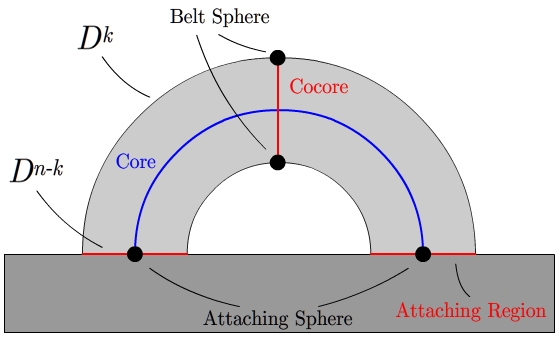
\includegraphics[scale=1.2]{graphics/handleanatomy}
\caption{Anatomy of an $n$-dimensional $k$-handle}
\label{handle anatomy}
\end{figure}

Unfortunately this picture is a little misleading since attaching a $k$-handle does not always look like attaching a ball along two disconnected pieces of its boundary. For example, attaching a 4-dimensional 2-handle means attaching a copy of $D^2 \times D^2$ along the solid torus $S^1 \times D^2$. The boundary of $D^2 \times D^2$ is a union of solid tori $S^1 \times D^2 \cup D^2 \times S^1$ that intersect at their boundaries $S^1 \times S^1$, and this decomposition of $S^3$ into two solid tori is clearly the genus 1 Heegaard splitting.




An embedding $\varphi : \partial D^k \times D^{n-k} \rightarrow \partial X$ is the same as embedding the trivial normal bundle of the attaching sphere $\varphi(\partial D^k \times 0)$ into $\partial X$. Therefore $\varphi$ determines, and is determined by, an embedding $\varphi_0 : \partial D^k \times 0 \rightarrow \partial X$ of the attaching sphere and an equivalence $f$ of the normal bundle $\nu \varphi_0(\partial D^k)$ with the trivial vector bundle $\partial D^k \times \mathbb R^{n-k}$; this is intuitively plausible, but is also the content of the Tubular Neighborhood Theorem. The embedding $\varphi_0$ is just a \textbf{knot} in $\partial X$, and the vector bundle equivalence $f$ is called a \textbf{(normal) framing} of $\partial D^k = S^{k-1}$. If the data $(\varphi_0,f)$ and $(\varphi_0',f')$ are smoothly isotopic, then the resulting manifolds $X \cup_\varphi h$ and $X \cup_{\varphi'} h$ are isotopic. 

Fix a framing $f_0$ for $S^{k-1}$, i.e. a vector bundle equivalence
\[
\xymatrix
{
	S^{k-1} \times \mathbb R^{n-k} \ar[r]^{f_0} \ar[d] & \nu \varphi_0(S^{k-1}) \ar[d] \\
	S^{k-1} \ar[r]_{\varphi_0} & \varphi_0(S^{k-1})
}
\]
If $f$ is another framing of $S^{k-1}$, then $f^{-1} \circ f_0 : S^{k-1} \times \mathbb R^k \rightarrow S^{k-1} \times \mathbb R^{n-k}$ must map $(p,v)$ to $(p,g(p) \cdot v)$, where $g : S^{k-1} \rightarrow \GL(n-k)$ is smooth. Without loss of generality we can assume that $g(p) = I$ for a fixed base point $p \in S^{k-1}$. Therefore each framing determines an element of the group $\pi_{k-1}(GL(n-k))$, which is isomorphic to $\pi_{k-1}(O(n-k))$ by the deformation retract of $GL(n-k)$ onto $O(n-k)$, and it is even true that the set of framings are in one-to-one correspondence with elements of $\pi_{k-1}(O(n-k))$. However, the set of framings is not canonically isomorphic to $\pi_{k-1}(O(n-k))$, since the identification depends on $f_0$, but it is a principal homogeneous space for $\pi_{k-1}(O(n-k))$. Sometimes there is a canonical choice of $f_0$, and this will be useful later.

We can get a lot of information about attaching very low index handles and very high index handles. The attaching sphere for a $0$-handle $D^0 \times D^n$ is empty, so attaching a $0$-handle to $X$ is the same as simply taking the disjoint union of $X$ with $D^n$. The attaching sphere of a $1$-handle is a disjoint pair of points, and so if $\partial X$ is connected and non-empty there is a unique isotopy class of attaching maps (well, except in the case $n=2$ and $\partial X$ non-compact, in which case we can also interchange the two components of the attaching sphere). Further, since $\pi_0(O(n-1)) = \mathbb Z/2$ for $n \geq 2$ there are exactly two framings on $S^0$, hence there are exactly two manifolds one can obtain by attaching a $1$-handle to a $0$-handle (these are the $n$-dimensional analogs of annulus and \Mobius band). 

Similarly, for $(n-1)$-handles, with $n \neq 2$, there is a unique framing of $S^{n-2}$ since $\pi_{n-2}(O(1)) = 0$. In the case $n=2$ we see that $(n-1)$-handles are just $1$-handles, which were discussed above. Attaching an $n$-handle is the same as gluing a copy of $D^n$ to $\partial X$ along $\partial D^n = S^{n-1}$. Since $\partial X$ is $(n-1)$-dimensional we see that we can only attach $D^n$ to boundary components of $X$ that are diffeomorphic to $S^{n-1}$. However, due to issues of exotic $n$-spheres and exotic diffeomorphisms of $n$-spheres we can only say that attaching an $n$-handle is unique in dimensions $\leq 6$. 

The other combinations of $k$ and $n$, where $k$ is neither small nor close to $n$, are harder to understand. If $n-k > 2$, then there is only one isotopy class of embeddings $S^{k-1}$ into $(n-1)$-dimensional manifolds, hence all embeddings can be ``unknotted.'' So, the only thing that controls what we get from attaching a $k$-handle to a $0$-handle is the framing of an unknotted sphere in $S^{n-1}$, which are of course parameterized by $\pi_{k-1}(O(n-k))$. Suppose we are attaching a $k$-handle $h_2 = D^k \times D^{n-k}$ to a $0$-handle $h_1 = D^n$ such that the attaching sphere is the standardly embedded, unknotted sphere $S^{k-1} \subset S^{n-1}$. Without loss of generality we can assume that we have an identification $h_1 = D^k \times D^{n-k}$ and that the attaching map of $h_1$ is of the form $\varphi : \partial D^k \times D^{n-k} \rightarrow \partial D^k \times D^{n-k} \subset D^n$ such that $\pi_{\partial D^k} \circ \varphi$ is the identity, and the restriction of $\varphi$ to any slice $\lcb * \rcb \times D^{n-k}$ is an orthogonal linear map. Let $X$ be the manifold $h_1 \cup_\varphi h_2$. We claim that there is a canonical map $\pi : X \rightarrow S^k$ making $X$ into a $D^{n-k}$-bundle. Decompose $S^k$ as a union of two discs, the upper and lower hemispheres. Then $\pi$ projects the handle $h_1$ onto its its first factor, which is then identified with the upper hemisphere, and $\pi$ projects $h_2$ onto its first factor, which is then identified with the lower hemisphere. It is clear that this makes $X$ into a $D^{n-k}$-bundle, and in fact all $D^{n-k}$-bundles are of this form. Further, consider the framing $f_0$ corresponding to $\id_{\partial D^k \times D^{n-k}}$. This clearly gives the trivial bundle $X = S^k \times D^{n-k}$, and so this is a canonical element to associate to the identity in $O(n-k)$.

If we apply the above discussion to the case $k=2$, then we have that $D^{n-2}$-bundles over $S^2$ are classified by $\mathbb Z$ if $n=4$ and by $\mathbb Z/2$ if $n>4$. In this case we can get a canonical identification of these bundles with $\mathbb Z$ ($n=4$) and $\mathbb Z/2$ ($n>4$) by associating the trivial bundle with 0. For $n=4$, the integer associated to a $D^2$ bundle over $S^2$ is called the Euler number of the bundle. If $n > 4$, then we denote the non-trivial $D^{n-2}$ bundle over $S^2$ by $D^{n-2} \tilde\times S^2$, and we also define the associated $S^{n-3}$ bundle over $S^2$ by $S^{n-3} \tilde\times S^2 = \partial (D^{n-2} \tilde\times S^2)$.


Let $X$ be a compact $n$-manifold with boundary written as $\partial_+ X \sqcup \partial_- X$. If $X$ is oriented give $\partial_+ X$ the induced orientation and $\partial_- X$ the opposite of the induced orientation. A \textbf{handlebody decomposition} of $X$ is an identification of $X$ with an $n$-manifold obtained by attaching handles to $\partial_- X \times I$ such that $\partial_- X$ is identified with $\partial_- X \times 0$. A manifold with such a decomposition is called a \textbf{relative handlebody} built on $\partial_- X$, or if $\partial_- X = \emptyset$ then $X$ is simply called a \textbf{handlebody}. 

The theory of handlebodies and Morse theory are closely related, so it is hard to discuss one without the other. Unfortunately we have now come to a point where we need to assume the reader has some knowledge of Morse theory. One can read this section concurrently with \cref{Morse Theory}.

According to the results in \cref{Morse Theory} we have that every smooth, compact $n$-manifold has a handlebody decomposition using Morse theory, and this can even be extended to non-compact manifolds with compact boundary. Amazingly every topological $n$-manifold with $n \neq 4$ also admits a handlebody decomposition, but this is not true in dimension $n=4$. For example, there is a 4-manifold with intersection form $E_8$ which does not admit a smooth structure or a handlebody decomposition.


\begin{prop}
\label{handlebodies with increasing index handles}
Any handlebody decomposition of a pair $(X,\partial_-X)$ can be modified (by isotoping attaching maps) so that handles are attached in order of increasing index, and handles of the same index can be attached in any order or simultaneously.
\end{prop}
\begin{proof}
Suppose we attach a $k$-handle $h_1$ and then an $\ell$-handle $h_2$ to a manifold $X$, with $\ell \leq k$. First we will perturb the attaching map of $h_2$ slightly so that its attaching sphere does not intersect $h_1$'s belt sphere (if needed). Note that $h_1$'s belt sphere, $0 \times \partial D^{n-k}$, is of dimension $n-k-1$ and $h_2$'s attaching sphere, $\partial D^\ell \times 0$, is of dimension $\ell-1$. The codimension of the intersection of generically positioned submanifolds is the sum of the submanifolds' codimension, so the codimension of $h_1$'s belt sphere intersected with $h_2$'s attaching sphere, in $\partial X$, is 
\[ (n-1)-(n-k-1) + (n-1)-(\ell-1) = n-1-n+k+1+n-1-\ell+1 = n + k-\ell \geq n \]
Hence we can perturb the attaching sphere of $h_2$ slightly so that the spheres become entirely disjoint. Now take a smooth vector field on $X \cup h_1$ emanating from the cocore of $h_1$ radially, and flow the attaching sphere of $h_2$ along this vector field. This will push the attaching sphere of $h_2$ to $\partial X$, so we can first attach $h_2$ and then $h_1$.
\end{proof}

We will always assume that our handlebodies are ordered so that handles are attached with increasing index, and we will write $X_k$ to denote $\partial_-X \times I$ union all the handles of index $\leq k$.

A handlebody decomposition of a pair $(X,\partial_- X)$ naturally leads to a dual handlebody decomposition of $(X,\overline{\partial_+ X})$, where $k$-handles in the first decomposition become $(n-k)$-handles in the second decomposition. When we attach a $k$-handle $h$ to $X$, the points in $\partial D^k \times D^{n-k}$ become interior points of $X \cup h$ and the points in $D^k \times \partial D^{n-k}$ become boundary points in $X \cup h$. Other handles will be attached to the part $D^k \times \partial D^{n-k}$ of $h$, so we could reverse this and instead think of $h$ has an $(n-k)$-handle being attached to those other handles. Intuitively, we are turning the handlebody upside down. If the handlebody decomposition is given by a Morse function $f$, then the dual handlebody is just the handlebody given by the Morse function $1-f$. 



\begin{example}
\label{handlebody decompositions of CP^n and RP^n}
We will show how $\mathbb CP^n$, complex projective $n$-space, can be decomposed into a handlebody with one $2k$-handle for each $0 \leq k \leq n$. Recall that $\mathbb CP^n$ is the quotient of $\mathbb C^{n+1}-0$ by $\mathbb C^*$ acting by scalar multiplication. The equivalence class of $(z_0,\ldots,z_n)$ is denoted by $[z_0:\cdots:z_n]$. Complex projective space is an $n$-dimensional complex manifold (or $2n$-dimensional real manifold) that can be covered with $n+1$ charts $\varphi_i : \mathbb C^n \rightarrow \mathbb CP^n$ defined by 
\[ \varphi_i(z_0,\ldots,z_{n-1}) = [z_0:\cdots:z_{i-1}:1:z_i:\cdots:z_{n-1}] \]
The inverses $\phi_i : U_i \rightarrow \mathbb C^n$ of these charts are given by
\[ \phi_i([z_0,\ldots,z_n]) = (z_0/z_i,\ldots,z_{i-1}/z_i,z_{i+1}/z_i,\ldots,z_n/z_i) \]
where $U_i$ consists of all points $[z_0,\ldots,z_n]$ such that $z_i \neq 0$. 

Let $D$ be the unit disc in $\mathbb C$, and and let $B_i = \varphi_i(D \times \cdots \times D)$ (an embedded complex $n$-ball in $\mathbb CP^n$). Every point $p \in \mathbb CP^n$ has a unique representative $(z_0,\ldots,z_n)$ such that $|z_i|=1$ for some $0 \leq i \leq n$ and $|z_j| \leq 1$ for all $j$ (just divide by the coordinate with largest norm), which we will call the canonical representative of $p$. It follows that $\lcb B_i \rcb$ covers $\mathbb CP^n$. We also see that $p \in B_i$ if and only its canonical representative has $|z_i|=1$, and $p \in \partial B_i$ if and only if $|z_j| = 1$ for some other $j \neq i$. From this it follows that two balls $B_i$ and $B_j$ can intersect only at points in the boundaries of each ball: $p \in B_i \cap B_j$ if and only if its canonical representative has $|z_i|=|z_j|=1$ and $|z_k| \leq 1$ for all $k$. In particular, then ball $B_k$ intersects the union $\cup_{i < k} B_i$ at all points whose canonical representative has $|z_k|=1$, $|z_j|=1$ for some $0 \leq j < k$ and $|z_\ell| \leq 1$ for all $\ell$. This means that the restriction of $\varphi_k$ to $\partial(D \times \cdots \times D) \times D \times \cdots \times D \subset D^k \times D^{n-k}$ is an embedding into $\cup_{i<k} B_i$, therefore $\cup_{i \leq k} B_i$ can be obtained from $\cup_{i<k} B_i$ by attaching a $2k$-handle via $\varphi_k$. 

By replacing $\mathbb R$ for $\mathbb C$ in the above construction we get a decomposition of $\mathbb RP^n$ into a handlebody with one $k$-handle for each $0 \leq k \leq n$. We are going to explicitly compute the attaching maps for $\mathbb RP^1,\mathbb RP^2,\mathbb CP^1$ and $\mathbb CP^2$. From the description above we have that $\mathbb RP^1$ is constructed by gluing $B_1 = \lcb [x,1] \st -1 \leq x \leq 1 \rcb$ to $B_0 = \lcb [1,x] \st -1 \leq x \leq 1 \rcb$ via the map $\varphi_1$ restricted to $\partial D \subset \mathbb R$. In this case $\varphi_1 : \lcb -1,+1 \rcb \rightarrow B_0$ and $\varphi_1(-1)=[-1,1]$ and $\varphi_1(1)=[1,1]$. This is the attaching map, and it attaches one interval to another by identifying endpoints, hence $\mathbb RP^1$ is just a circle.

The real projective plane $\mathbb RP^2$ can be written as a union of a 0-, 1- and 2-handle. From the construction we described we have the following balls
\begin{align*}
B_0 &= \lcb [1,x,y] \st -1 \leq x,y \leq 1 \rcb \\
B_1 &= \lcb [x,1,y] \st -1 \leq x,y \leq 1 \rcb \\
B_2 &= \lcb [x,y,1] \st -1 \leq x,y \leq 1 \rcb 
\end{align*}
We attach a 1-handle to $B_0$ via the map $\varphi_1|_{\partial D \times D}$, which maps $(\pm 1,x)$ to $[\pm 1,1,x] = [1,\pm 1,\pm x] \in B_1$. Explicitly, this means that $(1,x)$ is mapped to $[1,1,x]$ and $(-1,x)$ maps to $[1,-1,-x]$, so this is identifying edges of two squares with a twist (see \cref{rp2-attach-1-handle}). We attach a 2-handle to $B_0 \cup B_1$ via $\varphi_2|_{\partial(D \times D)}$ which maps $(\pm 1,x)$ to $[\pm 1,x,1] = [1,\pm x,\pm 1] \in B_0$ and maps $(x,\pm 1)$ to $[x,\pm 1,1] = [\pm x,1,\pm 1] \in B_1$. This glues a disc into $B_0 \cup B_1$ as in \cref{rp2-attach-2-handle}, where have not yet identified the final 2 sides of the square since that would make it difficult to draw $B_0 \cup B_1 \cup B_2$.


\begin{figure}[tb]
\centering
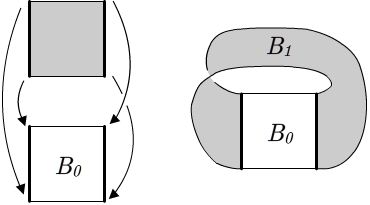
\includegraphics[scale=.6]{graphics/rp2-attach-1-handle}
\caption{Attaching the 1-handle in $\mathbb RP^2$}
\label{rp2-attach-1-handle}
\end{figure}



\begin{figure}[tb]
\centering
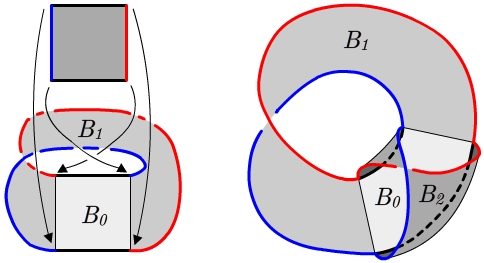
\includegraphics[scale=.65]{graphics/rp2-attach-2-handle}
\caption{Attaching the 2-handle in $\mathbb RP^2$}
\label{rp2-attach-2-handle}
\end{figure}

Now consider $\mathbb CP^1$, which is the union of a 0-handle and 2-handle. By definition we have
\begin{align*}
B_0 &= \lcb [1,z] \st |z|\leq 1 \rcb \\
B_1 &= \lcb [z,1] \st |z|\leq 1 \rcb 
\end{align*}
We attach a 2-handle to $B_0$ via $\varphi_1$ which maps $z$ to $[z,1] = [1,1/z] = [1,\conj{z}] \in B_0$. This means we attach two discs along the map $z \mapsto \conj{z}$, so $\mathbb CP^1$ is just the 2-sphere.

Finally, consider $\mathbb CP^2$, which is the union of a 0-handle, 1-handle and 2-handle. We have
\begin{align*}
B_0 &= \lcb [1,z,w] \st |z|,|w| \leq 1 \rcb \\
B_1 &= \lcb [z,1,w] \st |z|,|w| \leq 1 \rcb \\
B_2 &= \lcb [z,w,1] \st |z|,|w| \leq 1 \rcb
\end{align*}
We attach a 2-handle to $B_0$ via $\varphi_1$ restricted to $\partial D \times D$, which maps $(z,w)$ to $[z,1,w] = [1,1/z,w/z] = [1,\overline z,\overline zw] \in B_0$. The 4-handle is attached to $B_0 \cup B_1$ via the restriction of $\varphi_2$ to $\partial(D \times D)$, which maps $(z,w)$ to $[1,\overline zw,\overline z]$ on the $\partial D \times D$ part, and maps $(z,w)$ to $[z\overline w,1,\overline w]$ on the $D \times \partial D$ part.
\end{example}


There is a natural handlebody decomposition on the product of two handlebodies. Consider the simplest case
\[ X = D^m \cup_{\varphi_1} D^k \times D^{m-k} \ \ \ \ \ \varphi_1 : \partial D^k \times D^{m-k} \rightarrow \partial D^m \]
\[ Y = D^n \cup_{\varphi_2} D^l \times D^{n-l} \ \ \ \ \ \varphi_2 : \partial D^l \times D^{n-l} \rightarrow \partial D^n \]
Then $X \times Y$ has a handlebody decompositions into 0-handle $\cup$ $k$-handle $\cup$ $l$-handle $\cup$ $(k+l)$-handle. Let us figure out the attaching maps. The $k$-handle is attached via a map $\varphi_k : \partial D^k \times D^{m+n-k} \rightarrow \partial D^{m+n}$. If we write the domain as $\partial D^k \times D^{m-k} \times D^n$ and the range as $\partial D^m \times D^n \cup D^m \times \partial D^n$, then $\varphi_k = \varphi_1 \times \id$. In particular, the image of $\varphi_k$ lives in only the part $\partial D^m \times D^n$ of the boundary of $D^{m+n}$. We get something similar for the $l$-handle; its attaching map can be written as $\varphi_l = \id \times \varphi_1$. The $(k+l)$-handle is attached via a map $\varphi_{k+1} : \partial D^{k+l} \times D^{m+n-k-l} \rightarrow \partial D^{m+n}$. If we rewrite the domain as 
\[ \left( \partial D^k \times D^l \cup D^k \times \partial D^l \right) \times D^{m-k} \times D^{n-l} = \partial D^k \times D^{m-k} \times D^n \cup D^m \times \partial D^l \times D^{n-l} \]
and the range as before, then we can write $\varphi_{k+l} = \varphi_1 \times \id \cup \id \times \varphi_2$. This provides us with a general model for the product of handles in a product manifold.

Note that if the handlebody decompositions of $X$ and $Y$ are induced by Morse functions $f$ and $g$, respectively, then the product handlebody decomposition of $X \times Y$ is the same as the decomposition induced by the Morse function $h : X \times Y \rightarrow \mathbb R$ defined by $h(x,y) = f(x)+g(y)$. The critical points $(x,y) \in X \times Y$ of $h$ are precisely where $dh_{(x,y)} = df_x+dg_y = 0$, hence $df_x=0$ and $dg_y=0$ and so $x$ must be a critical point of $f$ and $y$ a critical point of $g$. If the critical point $x$ is of index $k$ and $y$ of index $l$, then $(x,y)$ is of index $k+l$, for the Hessian is of the form
\[ H_h(x,y) = \begin{pmatrix} \left( \frac{\partial^2 f}{\partial x^i \partial x^j} \right) & 0 \\ 0 & \left( \frac{\partial^2 g}{\partial y^i \partial y^j} \right) \end{pmatrix} = \begin{pmatrix} H_f(x) & 0 \\ 0 & H_g(y) \end{pmatrix} \]



\subsection{Handle Moves}
\label{Handle Moves}


Any manifold admits many ``different'' handlebody decompositions, so we want to find a set of moves that we could perform on handles in order to bring one handlebody presentation into another. First we show how to add a $(k-1)$-handle and $k$ in a specific way such that the result manifold does not change; that is, the handles cancelled each other. Let $X$ be an $n$-manifold with boundary. Write $\partial D^k$ as a union of upper and lower hemispheres, $S^{k-1} = D^{k-1}_+ \cup_{S^{k-2}} D^{k-1}_-$. Attach $D^k \times D^{n-k}$ to $\partial X$ via an embedding of $D_-^{k-1} \times D^{n-k}$ in $\partial X$ (this is \emph{not} attaching a $k$-handle). This does not change the diffeomorphism type of $X$ since it is just take the boundary sum of $X$ with an $n$ ball. We are going to show how to decompose this attached copy of $D^k \times D^{n-k}$ into a $(k-1)$-handle and $k$-handle. Let $J$ be a small neighborhood of $D_+^{k-1}$ in $D^k$, so that $J = D_+^{k-1} \times D^1$, and let $D_0^k$ be the disc left from slicing $J$ off of $D^k$. Then $J \times D^{n-k}$ is a $(k-1)$-handle attached to $\partial X$, and $D_0^k \times D^{n-k}$ is a $k$-handle attached to $\partial(X \cup J \times D^{n-k})$. This process of creating a pair of canceling handles is called \textbf{handle creation/cancellation}.

Sometimes it is possible to find a $(k-1)$-handle and $k$-handle that are situated in $X$ so that they cancel like the above. 

\begin{prop}
\label{handle cancellation}
A $(k-1)$-handle $h$ and a $k$-handle $h'$ can be cancelled if the attaching sphere of $h'$ intersects the belt sphere of $h$ transversely in a single point.
\end{prop}
\begin{proof}
\end{proof}

The process of finding two handles that cancel each other and canceling them from the handlebody is called \textbf{handle cancellation}. We can use handle cancellations to show that connected handlebodies can be made to have only one 0-handle and one $n$-handle.

\begin{prop}
If $X$ is a compact and connected $n$-manifold, then $X$ admits a handlebody decomposition with exactly one 0-handle and one $n$-handle.
\end{prop}
\begin{proof}
First we eliminate all 0-handles except for one. The 0-handles $X_0$ of $X$ is just a disjoint union of $n$-balls, and since $X$ is connected and since 1-handles are the only handles with disconnected attaching spheres, we have that each ball of $X$ must be connected to some other ball via a 1-handle. The attaching sphere of a 1-handle is a pair of points, and the belt sphere of a 0-handle is $S^{n-1}$, so it is clear by \cref{handle cancellation} that if a 1-handle connects two 0-handles then we can cancel one of the 0-handles and the 1-handle. Repeating this for all 1-handles connecting two 0-handles we can cancel all 0-handles except for one. 

Now that we have eliminated all 0-handles except for one, take the dual handlebody decomposition. This is a handlebody decomposition with a unique $n$-handle, but possibly many 0-handles. Apply the procedure from before to eliminate all 0-handles except for one and we are left with a handlebody with a unique 0- and $n$-handle.
\end{proof}


Let $(h_1,\varphi_1)$ and $(h_2,\varphi_2)$ be two $k$-handles with attaching maps, and suppose they are attached to $X$ simultaneously: $X \cup_{\varphi_ \cup \varphi_2} (h_1 \cup h_2)$. Let $A$ be the image of the attaching sphere of $h_1$ in $\partial X$ and $B$ the image of the belt sphere in $\partial X$. We can isotope the attaching map of $h_1$, which can also be thought of as isotoping the attaching sphere and the framing of the attaching sphere, and the resulting manifold will not change. By isotoping the attaching sphere we are, intuitively, ``sliding'' the handle $h_1$ around $\partial(X \cup h_2)$. Now, slide the attaching sphere of $h_1$ over the handle $h_2$ until the attaching sphere of $h_1$ intersects the belt sphere of $h_2$. Since the attaching sphere of $h_1$ is of dimension $k-1$ and the belt sphere of $h_2$ is of dimension $n-k-1$, we have that they will intersect at a point $p$, and $T_p A \oplus T_p B$ is a codimension 1 subspace of $T_p \partial(X \cup h_2)$. This means there are two directions we can move $A$ past $B$ (corresponding to the two components of the complement of the hyperplane $T_p A \oplus T_p B$). One direction will slide $h_1$ back to where we started. If we push $A$ the other way, and continue sliding $h_1$ until the attaching sphere lies entirely in $\partial X$, then we get a new handlebody which is the result of \textbf{sliding the handle $h_1$ over $h_2$}. Without loss of generality we can also assume that as we slide $h_1$ over $h_2$, the attaching sphere of $h_1$ stays inside some disc $D^k \times \lcb \text{pt} \rcb$ of $h_2$.

We have not change the manifold $X \cup h_1 \cup h_2$ by sliding the handle $h_1$ over $h_2$ (since we just isotoped the attaching sphere around), but the framing of $h_1$ might have changed in the process. For example, \cref{handle-slide} shows that sliding a trivially attached 1-handle across a twisted 1-handle results in another twisting. 

\begin{figure}[tb]
\centering
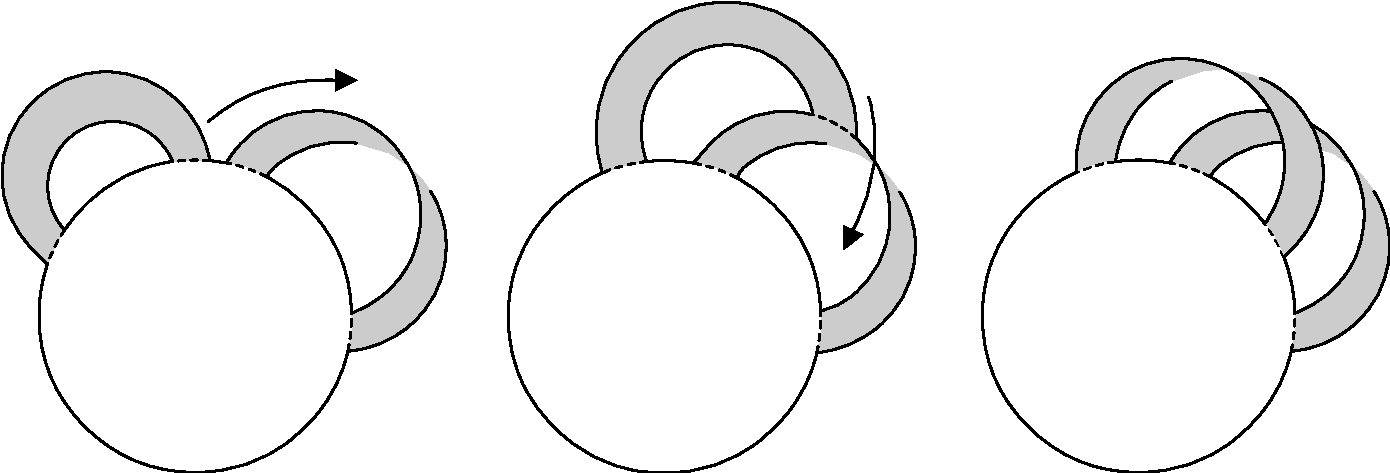
\includegraphics[scale=.6]{graphics/handle-slide}
\caption{A handle slide that changes the framing of a handle}
\label{handle-slide}
\end{figure}

It turns out these two moves on handlebody decompositions can always determine when two handlebody decompositions give the same manifold.

\begin{prop}
For any two relative handlebody decompositions of a compact pair $(X,\partial_- X)$ (with handles attaching in increasing order), it is possible to bring one decomposition into the other via a finite sequence of creation/cancellation of handle pairs, handle slides, and isotopies of attaching maps.
\end{prop}



\subsection{The Fundamental Group and Homology of a Handlebody}
\label{The Fundamental Group and Homology of a Handlebody}


The combinatorial presentation of a manifold as a handlebody immediately gives a presentation of the fundamental group of the manifold. Suppose $X$ is a handlebody with unique 0-handle, and give an orientation to the core of each 1-handle. We can make the oriented cores $D^1 \times 0$ into oriented loops in $X_1$ by connecting the end points with an oriented, straight line segment to the origin in $X_0 = D^n$. These loops are generators of the free group $\pi_1(X_1,x_0)$. As we attach 2-handles we will be adding relations to $\pi_1(X_1,x_0)$ to get $\pi_1(X_2,x_0)$. In particular, express the attaching circle $\partial D^2 \times 0$ of a handle in terms of the loops in $X_1$ to get the relation that attaching this 2-handle adds. Handles of higher index do not add any other relations since their attaching spheres are simply connected, so in particular $\pi_1(X_2,x_0) = \pi_1(X,x_0)$. Note that the above description of $\pi_1(X)$ is analogous to the presentation of $\pi_1(X)$ in terms of a CW-decomposition of a space. 

Next we develop a homology theory in terms of handlebodies, which is similar to cellular homology derived from a CW-complex. For a relative handlebody $(X,\partial_- X)$, let the $k$-chains of our homology theory be $C_k(X,\partial_-X) = H_k(X_k,X_{k-1})$, where $H_k(-,-)$ is just regular singular homology, hence $C_k(X,\partial_-X)$ can be thought of as formal linear combinations of $k$-handles (once the cores of the handles are given a fixed orientation). The boundary operator $\partial_k : C_k(X,\partial_-X) \rightarrow C_{k-1}(X,\partial_-X)$ is defined by the long exact sequence of the triple $(X_k,X_{k-1},X_{k-2})$. In particular, we have the following pieces of long exact sequences
\[ \cdots \longrightarrow H_k(X_k,X_{k-1}) \stackrel{\Delta_k}{\longrightarrow} H_{k-1}(X_{k-1}) \longrightarrow \cdots \]
\[ \cdots \longrightarrow H_{k-1}(X_{k-1}) \stackrel{j_*}{\longrightarrow} H_{k-1}(X_{k-1},X_{k-2}) \longrightarrow \cdots \]
where $\Delta_k$ is the connecting morphism and $j_*$ is induced by inclusion of the pairs $(X_{k-1},\emptyset) \hookrightarrow (X_{k-1},X_{k-2})$. Then we define $\partial_k = j_* \circ \Delta_k$, and clearly $\partial^2 = 0$ since $\Delta_k \circ j_* = 0$. If $X$ is oriented, then there is a more geometric definition of $\partial$. Let $h$ be a $k$-handle with attaching sphere $A$, and let $B_i$ be the belt sphere of each $(k-1)$-handle $h_i$. Then
\begin{equation}
\label{handlebody homology differential}
\partial_k h = \sum_i (A \cdot B_i) h_i
\end{equation}
where $A \cdot B_i$ is the intersection number computed in $\partial_+ X_{k-1}$. Since $\ker \partial \subset \image \partial$ we define $H_k(X) = \ker \partial_k / \image \partial_{k+1}$, and call this the \textbf{$k$-th handlebody homology group} of $X$ (this term is not standard). We can get a homology theory $H_k(X,\partial_-X;G)$ with coefficients in any abelian group $G$ by defining $C_k(X,\partial_-X;G) = C_k(X,\partial_-X) \otimes_{\mathbb Z} G$ with boundary operator $\partial \otimes \id$. We can also dualize this construction to get handlebody cohomology. In particular, set $C^k(X,\partial_-X;G) = \Hom(C_k(X,\partial_-X),G)$ and let $\delta^k : C^k(X,\partial_-X;G) \rightarrow C^{k+1}(X,\partial_-X;G)$ be the induced differential, and define $H^k(X,\partial_-X;G) = \ker \delta_k / \image \delta_{k-1}$. This is called the \textbf{$k$-th handlebody cohomology group} of $X$. If there is risk of confusing the handlebody chain and homology groups with other homology theories (such as singular homology), we may sometimes write them as $C_k^{HB}(X)$ and $H_k^{HB}(X)$. Further, if $\partial_-X=\emptyset$, then we will write these groups as $C_k(X;G),H_k(X;G)$, and so on.

Since handle moves do not change the diffeomorphism type of $X$ we have that the homology and cohomology groups will be the same. However, handle moves will add extra relations or change our canonical generators. Suppose a $k$-handle $h$ and $(k-1)$-handle $h_i$ form a canceling pair so that $A \cdot B_i = \pm 1$, where $A$ is the attaching sphere of $h$ and $B_i$ is the belt sphere of $h_i$. Then $\partial h = \pm h_i + \sum_{j \neq i} a_j h_j$ for some integers $a_j$. When we cancel these handles we will add the relations $h=0$ and $h_i = \mp \sum_{j \neq i} a_j h_j$ to the chain groups. On the other hand, sliding a handle $h$ across a handle $h'$ changes the canonical generators of $C_k(X)$ by replacing the basis element $h$ with $h \pm h'$.


\begin{example}
Since $S^n$ has a handlebody decomposition 0-handle $\cup$ 1-handle, we can easily see that its handlebody homology is $H_k(S^n)=\mathbb Z$ for $k=0,n$ and $0$ for $0 < k < n$. A more interesting example is writing $S^3$ as a union of a 0, 1, 2 and 3-handle, $S^3 = h_0 \cup h_1 \cup h_2 \cup h_3$. The standardly embedded solid torus $X_1 = S^1 \times D^2$ in $S^3$ is a 0-handle $\cup$ 1-handle. The attaching circle of the 2-handle we attach to $X_1$ is just the longitude $S^1 \times \lcb * \rcb$, where $*$ is any point on the boundary of $D^2$, and let $X_2$ be the result of this attachment. Then $\partial X_2$ is just $S^2$, and so we attach the 3-handle in the only way possible, and the result is $X_3 = S^3$.

We have $C_i(X) = \mathbb Z\< h_i \>$. Since there are no $(-1)$-handles, we have $\partial_0 = 0$. The attaching sphere of $h_1$ intersects the belt sphere of $h_0$ at two points, but different signs, so $\partial_1(h_1) = 0$. The attaching sphere of $h_2$ intersects the belt sphere of $h_1$ at one point, which we can arrange to have intersection number $+1$, hence $\partial_2(h_2)=h_1$. Finally, the attaching sphere of $h_3$ intersects the belt sphere of $h_2$ at two points, but with different signs, so $\partial_3(h_3) = 0$. Taking homology we see again that $H_0(S^3)=H_3(S^3)=\mathbb Z$ and $H_1(S^3)=H_2(S^3)=0$. 
\end{example}

\comment{
\begin{example}
We saw in \cref{handlebody decompositions of CP^n and RP^n} that $\mathbb RP^n$ admits a handlebody decomposition with one $k$-handle for each integer $0 \leq k \leq n$, hence $C_k(\mathbb RP^n) = \mathbb Z$. As we can see in \cref{rp2-attach-1-handle} and \cref{rp2-attach-2-handle}, the attaching sphere of the $k$-handle intersects the belt sphere of the $(k-1)$-handle in two points with the same sign, therefore $\partial_k(h_k) = \pm h_{k-1}$. All the boundary operators will be either multiplication by $+2$ or $-2$, therefore 
\[ H_k(\mathbb RP^n) = \frac{\ker \partial_k}{\image \partial_{k+1}} \]
\end{example}
}

\begin{example}
We saw in \cref{handlebody decompositions of CP^n and RP^n} that $\mathbb CP^n$ admits a handlebody decomposition with one $k$-handle for each even integer $k$ between $0$ and $2n$. So $C_{k}(\mathbb CP^n)=\mathbb Z$ for all even $0 \leq k \leq 2n$, and 0 for all other $k$. This implies that all the differentials are zero, hence $H_k(\mathbb CP^n) = C_k(\mathbb CP^n)$.
\end{example}




\subsection{2-Dimensional Handlebodies}
\label{2-Dimensional Handlebodies}



Two dimensional handlebodies have simple descriptions since there are so few ways to attach 2-dimensional $k$-handles ($k=0,1,2$). The 0- and 2-handles are just 2-discs, and a 1-handle is a band $I \times I$. The attaching region of this band consists of two disjoint intervals $I \sqcup I$, and there are two ways to attach the band to a 0-handle: without a twist, or with a twist. Once the 1-handles are attached, there is a unique way to attach the 2-handles so that we get a closed surface (just fill the holes!), so we can draw diagrams of 2-dimensional handlebodies by just drawing the 0-handle $\cup$ 1-handles. Some examples of these decompositions are shown in \cref{2-dimensional handlebody diagrams}, where the first image is $\mathbb RP^2$, the second is $T^2 \# \mathbb RP^2$, and the third is $T^2$. 

\begin{figure}[tb]
\centering
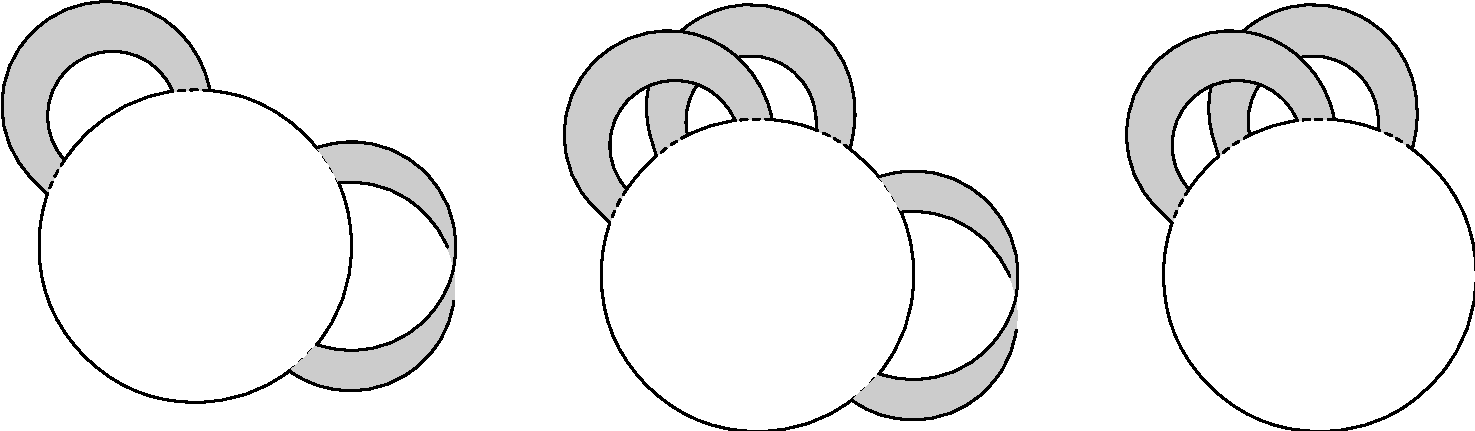
\includegraphics[scale=.6]{graphics/2-dim-handlebody-diagram}
\caption{Examples of 2-dimensional handlebody diagrams}
\label{2-dimensional handlebody diagrams}
\end{figure}





\subsection{Heegaard Diagrams}
\label{Heegaard Diagrams}


Heegaard splittings are an old method for constructing 3-manifolds, and we will see that it is equivalent to 3 dimensional handlebody. Although we get nice combinatorial pictures for 3 dimensional handlebodies, called Heegaard diagrams, they were still difficult to use. However, much later, many invariants were built from Heegaard diagrams, including a recent variation of Lagrangian Floer homology, which provides powerful invariants of 3- and 4-manifolds. 

We define a \textbf{handlebody of genus $g$} to be a 0-handle $\cup$ 1-handles such that the result is orientable, i.e. the interior (in the Jordan sense) of an orientable, genus $g$ surface. If $H_1$ and $H_2$ are handlebodies of genus $g$, then for any orientation-reversing homeomorphism $\varphi : \partial H_1 \rightarrow \partial H_2$ of their boundaries, we can form the orientable, compact 3-manifold $H_1 \cup_\varphi H_2$. Conversely, given a 3-manifold $M$, it is always possible to find a pair of embedded submanifolds $H_1,H_2$, both homeomorphic to a handlebody of genus $g$, such that $\partial H_1 = \partial H_2$ (this is proved below). In either case we call this a \textbf{Heegaard splitting}, or \textbf{Heegaard decomposition}, of the 3-manifold.
\begin{thm}
\label{existence of heegaard splitting}
Every compact, orientable 3-manifold admits a Heegaard splitting.
\end{thm}
\begin{proof}
We will give two different proofs.

\begin{itemize}

	\item The first proof is more geometric, using the fact that every 3-manifold has a triangulation. Let $K$ be a triangular of $M$, and let $K'$ and $K''$ denote the first and second barycentric subdivision of $K$ respectively. Let us recall how the barycentric subdivision is defined. Take a 2-face $\sigma$ in the triangulation and connect, with a new edge, the barycenter of $\sigma$ with each vertex of $\sigma$ and the midpoint of each edge of $\sigma$. This divides $\sigma$ into 6 new 2-faces. Then we can divide each 3-face $\rho$ into 24 new 3-faces by coning the barycenter of $\rho$ over each subdivided face of $\rho$. Performing this operation on all faces of $K$ gives us a new triangulation of $M$, called the first barycentric subdivision $K'$. Performing this operation again gives us the second barycentric subdivision $K''$.
	
	Let $H_1$ be the union of the 3-faces in $K''$ that do not intersect the 1-faces of $K$, and let $H_2$ be the closure of the complement of $H_1$. Then $H_1$ and $H_2$ are handlebodies which intersect precisely at their boundaries. This gives a Heegaard splitting of $M$.
	
	\item The second proof is Morse theoretic, and is the beginning of more versatile methods in low dimensional topology via Morse theory. As we will see later (\cref{existence of self-indexing Morse functions}), any smooth manifold admits a self-indexing Morse function $f : M \rightarrow [0,n]$ with unique index 0 and index $n$ critical points. Let $f : M \rightarrow \mathbb [0,3]$ be such a Morse function for our 3-manifold, and let $H_1 = f^{-1}[0,3/2]$ and $H_2=f^{-1}[3/2,3]$. If $f$ has $g$ index 1 critical points, then $H_1$ is a 0-handle with $g$ 1-handles attached, hence a genus $g$ handlebody. If we dualize the handlebody decomposition we see that $H_2$ is a 0-handle with $h$ 1-handles attached, where $h$ is the number of index 2 critical points. Since $\partial H_2 = \partial H_1 = $ a surface of genus $g$, we have that $g=h$, and so $H_2$ is also a handlebody of genus $g$. Therefore $M$ has been expressed as a union of two handlebodies along their boundary.
	
\end{itemize}
\end{proof}


The proof of \cref{existence of heegaard splitting} is a little discouraging since any manifold admits many triangulations, and hence many splittings. But, there is a nice combinatorial picture to help us understand the structure of a Heegaard splitting. Let $H_1$ and $H_2$ be two copies of the standardly embedded handlebody (see \cref{standardly embedded handlebody}), and let $\Sigma$ be the standardly embedded surface of genus $g$. Take an orientation-preserving homeomorphism $\varphi_1 : \partial H_1 \rightarrow \Sigma$ and an orientation-reversing homeomorphism $\varphi_2 : \partial H_2 \rightarrow \Sigma$, and form the compact, orientable 3-manifold $M = H_1 \cup_{\varphi_2^{-1} \circ \varphi_1} H_2$. Let $\alpha_1,\ldots,\alpha_g$ be the image of the standard circles in $\Sigma$ (the thin circles in \cref{standardly embedded handlebody}) under $\varphi_1$, and $\beta_1,\ldots,\beta_g$ the image of the standard circles in $\Sigma$ under $\varphi_2$. The curves $\alpha_1,\ldots,\alpha_g$ are collectively known as the $\alpha$-curves, and are mutually disjoint, and the curves $\beta_1,\ldots,\beta_g$ are collectively known as the $\beta$-curves, and are also disjoint. 

\begin{figure}[tb]
\centering
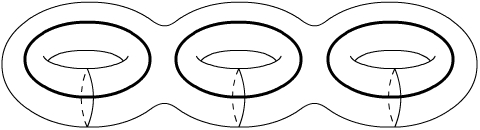
\includegraphics[scale=.5]{graphics/standardhandlebody}
\caption{Standardly embedded handlebody}
\label{standardly embedded handlebody}
\end{figure}


We now have a picture associated to any Heegaard decomposition: its a surface with $2g$ curves drawn on it. Many times we will take one of the collections of curves to be the standard curves, which would mean that $\varphi_1$ or $\varphi_2$ is just the identity, in which case we will not even draw them. The data of the surface $\Sigma$ with these $2g$ embedded curves is called the \textbf{Heegaard diagram} of the splitting. We would like to know that these embedded curves somehow uniquely determine the 3-manifold obtained from gluing the handlebodies together, but first we state a small technical lemma that will be used repeatedly in these notes.

\begin{lem}
\label{technical gluing lemma}
Let $X$ and $Y$ be two $n$-manifolds with homeomorphic boundaries, and let $Z = X \cup_f Y$ be the space formed by gluing $X$ and $Y$ together along a homeomorphism $f : \partial X \rightarrow \partial Y$. If $\tau : \partial X \rightarrow \partial X$ is any homeomorphism that extends to a homeomorphism $\widetilde \tau : X \rightarrow X$, then $Z$ is homeomorphism to $Z' = X \cup_{f \circ \tau} Y$.
\end{lem}
\begin{proof}
There are embeddings of $X$ and $Y$ into $Z$ by sending a point to its equivalence class in $Z$. If $x \in X,y \in Y$ are in the interior, then the corresponding points in $Z$ are $[x]=\lcb x \rcb$ and $[y]=\lcb y \rcb$, whereas if $x \in X,y \in Y$ are boundary points, then $[x]=\lcb x,f(x) \rcb$ and $[y] = \lcb y,f^{-1}(y) \rcb$. Let $\widetilde X$ and $\widetilde Y$ denote the images of $X$ and $Y$ under these embeddings so that $\widetilde X \cap \widetilde Y$ is just the set of equivalence classes with representative in $\partial X$ or $\partial Y$. We define a map $g : Z \rightarrow Z'$ on a point $z$ in $X$ or $Y$ by the following
\[ g(z) = \begin{cases}
				[\widetilde \tau^{-1}(x)] & z \in \widetilde X \\
				[y] & z \in \widetilde Y
			\end{cases}
\]
where $x \in X$ and $y \in Y$ are representatives of $z$. This map is clearly well-defined. In order for it to be continuous we need $[\widetilde \tau^{-1}(x)] = [y]$ in $Z'$ for any $z=\lcb x,y \rcb$ in $\widetilde X \cap \widetilde Y$ (i.e. $y=f(x)$). This is easy to see for on one side we have
\[ [\widetilde \tau^{-1}(x)] = [\tau^{-1}(x)] = \lcb \tau^{-1}(x),f(\tau(\tau^{-1}(x)) \rcb = \lcb \tau^{-1}(x),f(x) \rcb \]
and on the other side we have
\[ [y] = [f(x)] = \lcb \tau^{-1}(x),f(x) \rcb \]
Therefore the map is continuous, and now it is clear that it is even a homeomorphism.
\end{proof}

\begin{thm}
\label{isomorphic heegaard diagrams give homeomorphic manifolds}
The homeomorphism type of the manifold resulting from gluing two handlebodies together depends only on the image of the standard meridians under the gluing map, hence equal Heegaard diagrams describe homeomorphic manifolds.
\end{thm}
\begin{proof}
Suppose we are gluing genus $g$ handlebodies $H_1$ and $H_2$ together via a homeomorphism $f : \partial H_1 \rightarrow \partial H_2$. We can glue these handlebodies together in a two step process. First, let $\alpha_1,\ldots,\alpha_g$ denote a small tubular neighborhood of each standard meridian in $H_1$ (hence these are annuli), and let $D_1,\ldots,D_g$ denote the thickened discs these annuli bound in $H_1$. Then we can first attach the discs $D_i$ to $H_2$ via $f$ to obtain the intermedia space $M'$. Now we are left with attaching $H_1 \backslash (D_1 \cup \cdots \cup D_g)$ to $M'$, but this is topologically a ball, and so any homeomorphism from the boundary of this ball to $\partial M'$ (which is just a sphere) can be extended to the interior of the ball, and hence any gluing map will give a homeomorphic space by the above gluing lemma. Therefore the homeomorphism type of $H_1 \cup_f H_2$ depends only on the images of the $\alpha_i$ curves.
\end{proof}


We can also define Heegaard diagrams axiomatically. Let us temporarily say that an \emph{$H$-diagram} is a surface $\Sigma$ of genus $g$ and embedded curves $\alpha_1,\ldots,\alpha_g,\beta_1,\ldots,\beta_g$ such that the $\alpha$-curves are disjoint and the complement of their union is connected, and similarly for the $\beta$-curves.
\begin{thm}
An $H$-diagram $(\Sigma,\alpha_1,\ldots,\alpha_g,\beta_1,\ldots,\beta_g)$ corresponds to the Heegaard diagram of some splitting.
\end{thm}
\begin{proof}
Let $\alpha_i,\beta_i$ be curves with the above properties. First we claim that cutting $\Sigma$ along the $\alpha$-curves yields a 2-sphere with $2g$ holes. Suppose that $\Sigma$ with the $\alpha$-curves removed is a surface of genus $h$ with $2g$ holes. Then its Euler characteristic would be $2-2h-2g$. On the other hand, removing circles from surfaces that do not separate the surface does not change the Euler characteristic, so we should have $2-2g=2-2h-2g$, hence $h=0$, and so $\Sigma \backslash \alpha_1,\ldots,\alpha_g$ is a sphere with $2g$ holes.

Since $\Sigma$ with the removed $\alpha$-curves is just a sphere with $2g$ holes, we can homeomorphically deform it so that it is in the standard position of a handlebody of genus $g$ with its standard circles cut out. Now it is easy to find a handlebody of genus $g$ with homeomorphism of its boundary onto $\Sigma$ taking its standard circles to the $\alpha$-circles. This can be done for the $\beta$ curves in the same way.
\end{proof}

Therefore $H$-diagrams and Heegaard diagrams are equivalent notions, so we will refer to both as Heegaard diagrams from now on. The condition that the complement of the union of the $\alpha$-curves in $\Sigma$ is connected is equivalent to saying that the homology classes of $\alpha_1,\ldots,\alpha_g$ span a rank $g$ submodule of $H_1(\Sigma) \cong \mathbb Z^{2g}$. 

There is also a Morse theoretic way of thinking of Heegaard diagrams. Let $f : M \rightarrow [0,3]$ be a self-indexing Morse function with unique maximum and minimum, and let $H_1 = f^{-1}[0,3/2]$, $H_2 = f^{-1}[3/2,3]$ and $\Sigma = f^{-1}(3/2)$. By \cref{existence of heegaard splitting} we know that $H_1$ and $H_2$ are handlebodies of the same genus, say $g$. Let $P_1,\ldots,P_g$ be the index 1 critical points of $f$, and $Q_1,\ldots,Q_g$ be the index 2 critical points. Let $\alpha_i$ consist of the points that flow to $P_i$ under $-\nabla_g f$, and let $\beta_i$ consist of the points that flow to $Q_i$ under $+\nabla_g f$. Then $\Sigma(\alpha_1,\ldots,\alpha_g,\beta_1,\ldots,\beta_g)$ is a Heegaard diagram for $M$.

\begin{example}
There is only one Heegaard splitting of genus 0. In this case we have a manifold $M$ expressed as $M = D_1 \cup D_2$ where $D_1,D_2$ are 3-balls. Let $\varphi : D_1 \rightarrow S^3$ be an embedding of the first 3-ball onto the upper-hemisphere of $S^3$. The restriction of $\varphi$ to $\partial D_1 = \partial D_2$ can be extended to a homeomorphism from $D_2$ to the lower-hemisphere of $S^3$ (by Alexander's lemma). Pasting these homeomorphisms together gives a homeomorphism of $M$ with $S^3$, hence all genus 0 Heegaard splittings are $S^3$. 
\end{example}

\begin{example}
The standard Heegaard splitting of $S^3$ is to take the standardly embedded solid torus $H_1$ in $S^3$, and let $H_2$ be the complement of $H_1$ in $S^3$. The gluing map is just the identity. The standard orientation on $S^3$ induces orientations on $H_1$ and $H_2$. If we let $n$ denote the outward pointing normal vector field on $\partial H_1$, then the orientation of $H_1$ induces an orientation on $\partial H_1$ by choosing the equivalence class of bases at a tangent space such that adding $n$ gives the equivalence class of bases from the induced orientation on $H_1$. Do something similar to get an orientation on $\partial H_2$ induced by $H_2$. Clearly the two orientations induced on $\partial H_1 = \partial H_2$ are different, therefore the gluing map is orientation reversing. This is why we require the gluing map to be orientation reversing in our definition of Heegaard splitting.
\end{example}

\begin{example}
\label{Heegaard splitting description of lens spaces}
We can also classify all genus 1 splittings. All such splittings are given by an orientation reversing homeomorphism $f : T \rightarrow T$, and the isotopy classes of these maps are in bijective correspondence with integer matrices
\[ A = \begin{pmatrix} -q & r \\ p & s \end{pmatrix} \ \ \ \ \ \det A = pr + qs = 1 \]
so $p$ and $q$ are relatively prime or one is 0 and the other is $\pm 1$. We use $-q$ here because we required our gluing homeomorphism to be orientation reversing, so the determinant of this matrix should be $-1$, which can be written simply as $pr + qs = 1$ with our sign choice. This homeomorphism maps the meridian $\mu$ to the curve $-q \cdot \mu + p \cdot \lambda$, i.e. the meridian wraps $-q$ times around the meridian and $p$ times around the longitude. Let $M$ be the manifold resulting from gluing to copies of the solid torus via $f$. It is easy to see that $M$ depends only on the image of $\mu$ under $f$ by using an argument similar to \cref{isomorphic heegaard diagrams give homeomorphic manifolds}. Thus, $M$ is completely determined by the relatively prime pair of integers $(p,q)$, and we call this space the \textbf{$(p,q)$ Lens space} and denote it by $L(p,q)$.

The Heegaard diagram of $L(p,q)$ is just a curve on the torus that wraps $-q$ times around the meridian and $p$ times around the longitude. One can prove that $L(p,q) = L(-p,q)$ and $L(p,q) = L(p,q+np)$ for any integer $n$, so we can assume $p \geq 0$ and $0 \leq q \leq p-1$. But, if $p=0$ then we are forced to have $q=\pm 1$, and if $q=0$ we are also forced to have $p=\pm 1$. In these cases we have $L(\pm 1,n)=S^3$ for all integers $n$ and $L(0,\pm 1)=S^1\times S^2$, so disregarding these examples we can assume $p \geq 2$ and $1 \leq q \leq p-1$. We also have $L(2,1) = \mathbb RP^3$.

\begin{figure}[tb]
\centering
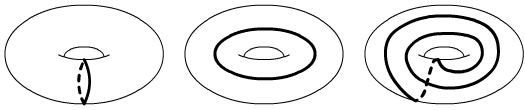
\includegraphics[scale=.6]{graphics/s1xs2-s3-rp3-hd}
\caption{Heegaard diagrams of $S^1 \times S^2, S^3, \mathbb RP^3$ respectively}
\label{s1xs2-s3-rp3-hd}
\end{figure}
\end{example}

\begin{example}
Heegaard diagrams can be quite complicated, for example see \cref{hd1}. We will show later that this 3-manifold is simply connected.

\begin{figure}[tb]
\centering
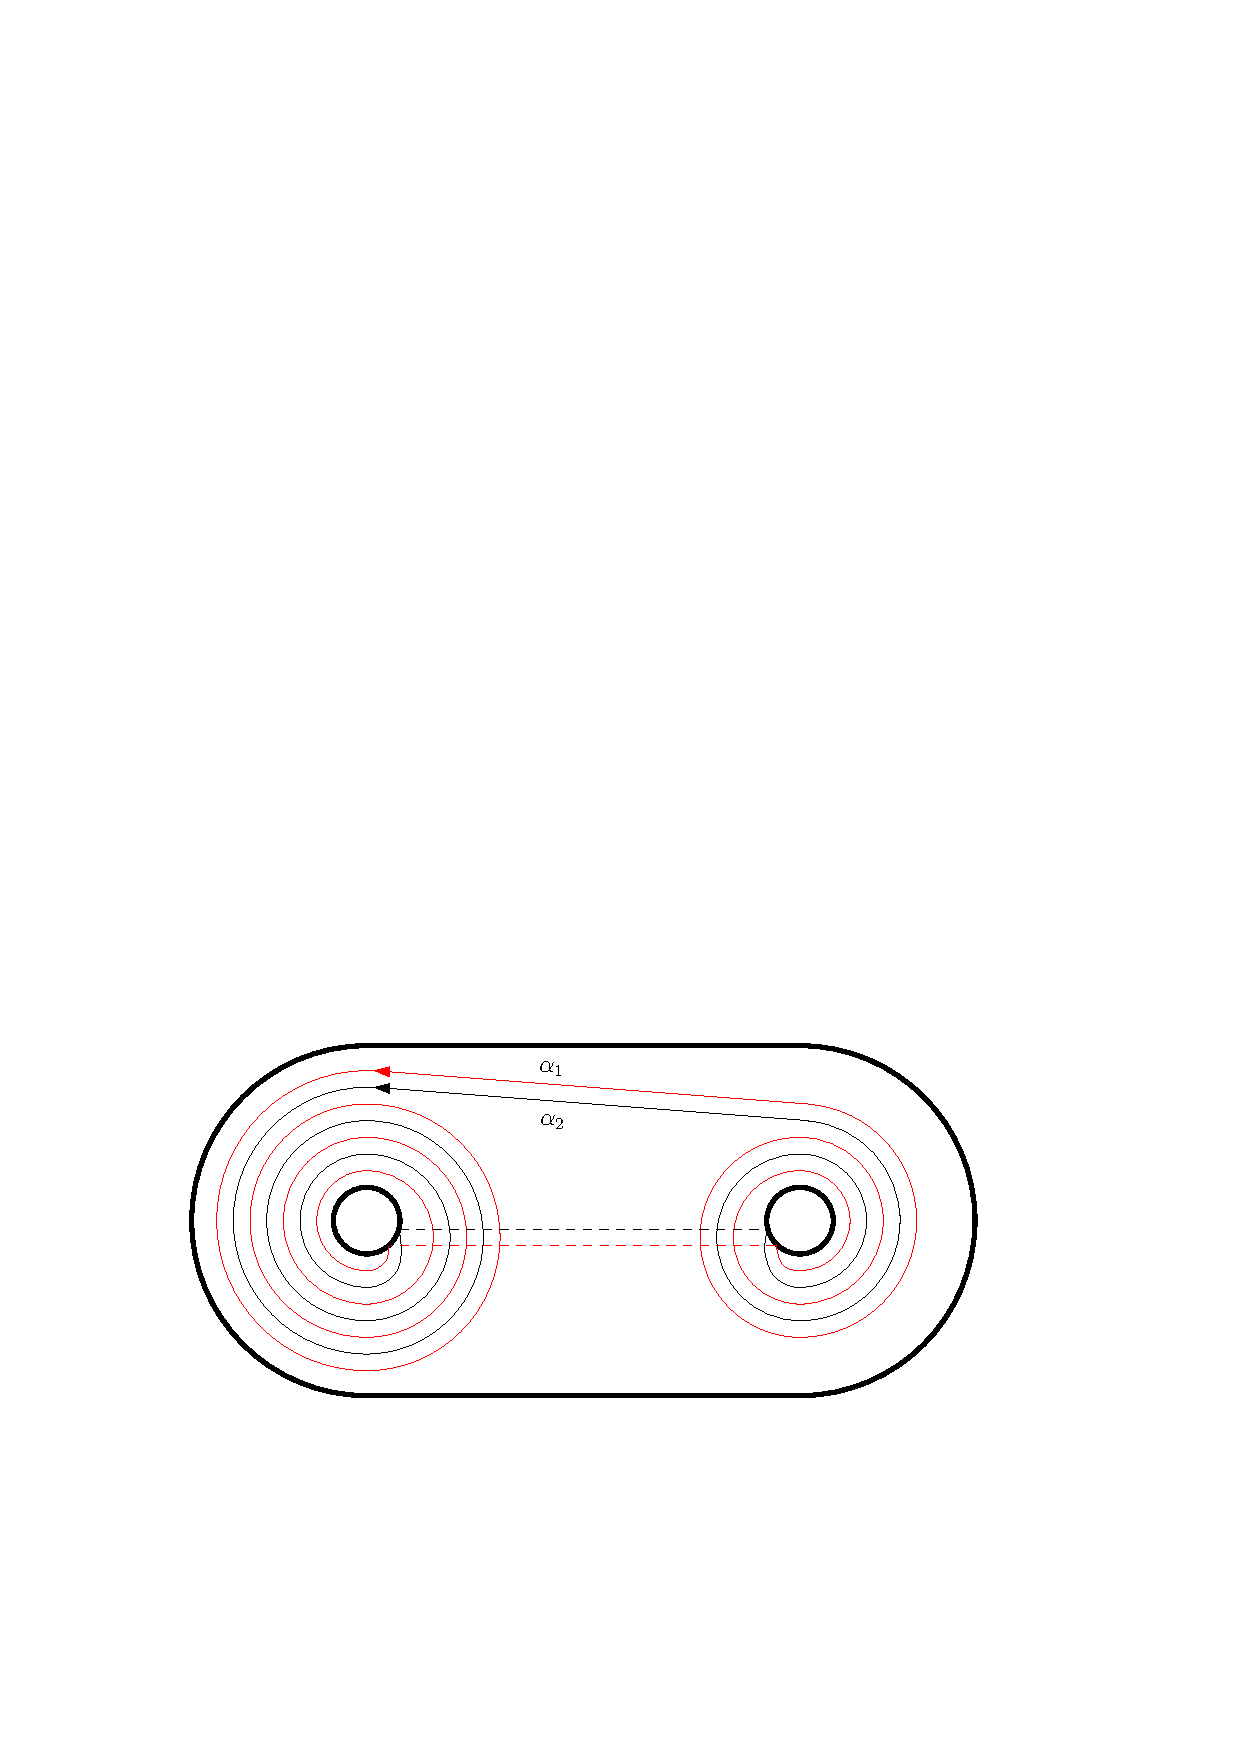
\includegraphics[scale=.9]{graphics/hd1}
\caption{Heegaard diagram of a simply connected 3-manifold}
\label{hd1}
\end{figure}
\end{example}




Let us reconcile the above theory of Heegaard splittings of 3-manifolds with our general theory of handlebodies. A handlebody of genus $g$ is a 0-handle $\cup$ 1-handles such that the result is orientable. This is just the first step in building a 3-dimensional handlebody, so let us denote it by $X_1$. Next we could attach some 2-handles (we certainly cannot attach a 3-handle yet, unless $g=0$). Attaching a 2-handle is completely determined by the image of the attaching sphere $\partial D^2 \times 0$ (which we will call the attaching circle in this case) and the framing of the attaching circle, which are parameterized by $\pi_1(O(1))=0$. Therefore, attaching the 2-handles is equivalent to specifying a collection of embedded circles in $X_1$, which is just a Heegaard diagram, and let $X_2$ be the result. If $\partial X_2$ is a collection of $S^3$'s, then there is a unique way to cap these off with 3-handles so that the result is a closed 3-manifold. This is precisely the case we draw $g$ embedded curves on $X_1$ such that the complement of their union is connected, so such a picture uniquely determines a 3-manifold.

Now we see that a Heegaard splitting is simply a 3-dimensional handlebody, and a Heegaard diagram is just a collection of curves drawn on $X_1$, we would like to translate our machinery of handle moves, handlebody homology and computation of fundamental groups into the Heegaard setting. We start with handle moves. We fix $X_1$ to be the standardly embedded handlebody of genus $g$ since all the information in a 3-dimensional handlebody is in the attaching circles of the 2-handles. In the handlebody theory we could isotopy the attaching maps, which just means that we can isotopy the $\alpha$ and $\beta$ curves on the surface of genus $g$. To create a canceling pair of 1- and 2-handles simply increase the genus of $X_1$ by one (i.e. add a 1-handle) and add the attaching circle that goes once around the longitude of the new 1-handle but does not venture into the old part of $X_1$. Attaching the 2- and 3-handles to this new Heegaard diagram will give the original manifold connect summed with $S^3$ (recall the Heegaard diagram of $S^3$, \cref{s1xs2-s3-rp3-hd}), hence it will be diffeomorphic to the original manifold.

Handle slides are a little more difficult to understand. Sliding the 1-handles is very simple, and does not produce anything interesting since we required $X_1$ to be orientable, hence allowed only one type of framing on the 1-handles. To get a feeling for sliding 2-handles, consider sliding two handles that are attaching to $D^3$. \Cref{sliding-3dim-2handles} shows how to do this in the obvious way. Here we sliding the attaching circle of one handle through the disc $D^2 \times \lcb 1 \rcb$ of the other handle. A better way to look at this is just to look at the attaching circles. Then we see that sliding 2-handles is equivalent to taking a parallel of one circle, and forming the banded sum of this circle with the other attaching circle (see \cref{sliding-3dim-2handles-2}). 

Now to slide a 2-handle $h_1$ across another 2-handle $h_2$ in a Heegaard diagram make a parallel copy of the attaching circle $\alpha_2$ of $h_2$ and form the \emph{band sum} of the attaching circle $\alpha_1$ of $h_1$ with the parallel of $h_2$. If we let $\gamma$ denote the band sum of $\alpha_1$ and the parallel of $\alpha_2$, then note that $\alpha_1,\alpha_2,$ and $\gamma$ bound a pair of pants in $X_1$. Conversely, if there are two attaching circles $\alpha_1,\alpha_2$ on $\partial X_1$ and another curve $\gamma$ on $\partial X_1$ such that $\gamma$ does not intersect any other attaching curves and $\alpha_1,\alpha_2,$ and $\gamma$ bound a pair of pants, then we can discard any one of these three curves without changing the resulting 3-manifold. See \cref{sliding-3dim-2handles-3} for a non-trivial example of this.


\begin{figure}[tb]
\centering
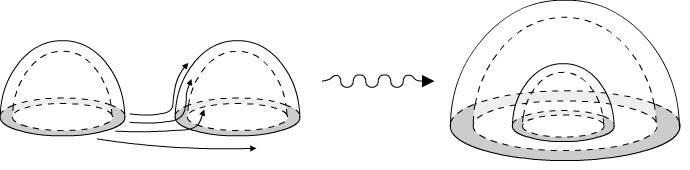
\includegraphics[scale=.6]{graphics/sliding-3dim-2handles}
\caption{Sliding 3-dimensional 2-handles}
\label{sliding-3dim-2handles}
\end{figure}

\begin{figure}[tb]
\centering
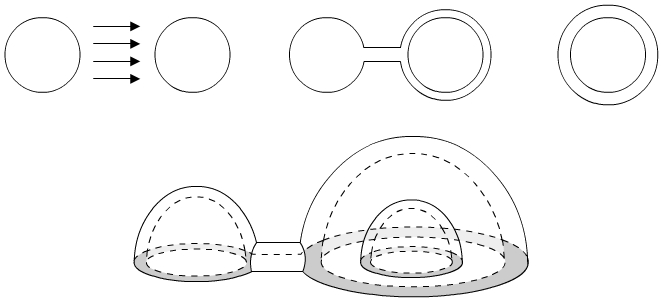
\includegraphics[scale=.6]{graphics/sliding-3dim-2handles-2}
\caption{Sliding 3-dimensional 2-handles}
\label{sliding-3dim-2handles-2}
\end{figure}

\begin{figure}[tb]
\centering
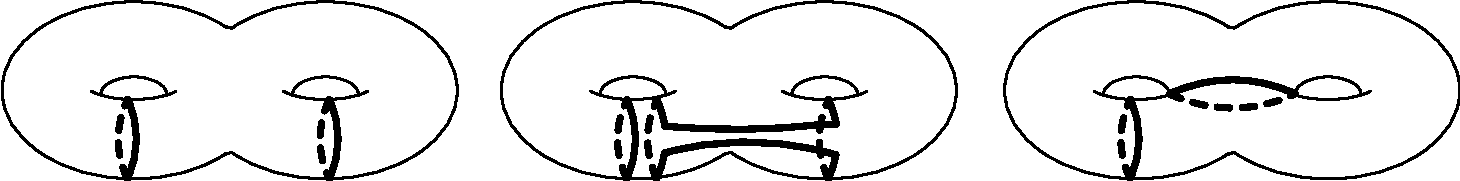
\includegraphics[scale=.6]{graphics/sliding-3dim-2handles-3}
\caption{Sliding 3-dimensional 2-handles}
\label{sliding-3dim-2handles-3}
\end{figure}


Next we see how to compute the fundamental group of a 3-manifold $X$ from one of its Heegaard diagrams. Choose a basis $x_1,\ldots,x_g$ for the free group $\pi_1(X_1)$, and let $r_i$ be the word in $x_1,\ldots,x_g$ representing the $i$-th attaching circle. Then a presentation of $\pi_1(X)$ is simply $\< x_1,\ldots,x_g \st r_1,\ldots,r_g \>$. 

\begin{example}
Consider the Heegaard diagram in \cref{hd1}. Let $x_1$ denote the standard generator around the first hole (counter-clockwise orientation) and $x_2$ the generator around the second hole (counter-clockwise orientation). One can easily check that the curve $\alpha_1$ is represented by the curve $x_1^3 x_2^2$ and $\alpha_2$ is represented by the curve $x_1^4 x_2^3$. Therefore a presentation for the manifold $M$ associated to this Heegaard splitting is $\pi_1(M) = \< x_1,x_2 \st x_1^3 x_2^2 = x_1^4 x_2^3 = 1 \>$. The first relation implies that $x_1^3 x_2^3 = x_2$, and plugging this into the second relation gives $x_1 x_2 = 1$. Therefore $x_1$ and $x_2$ are inverses in $\pi_1(M)$, hence $1=x_1^3 x_2^2 = x_1$ and $x_2=1$, and so $M$ is simply connected. 
\end{example}

Now we compute the homology of a 3-manifold $X$ from one of its Heegaard diagrams. We clearly have $H_0(X) = H_3(X) = \mathbb Z$, $C_1(X) = C_2(X) = \mathbb Z^g$ (if $X$ has $g$ 1- and 2-handles). Further, $\partial_1=0$ since the attaching spheres of the 1-handles intersect $\partial D^3$ at two points of opposite sign, and $\partial_3=0$ for similar reasons. Hence all the homology information of $X$ is contained in $\partial_2$. Given a 2-handle $h$, $\partial_2 h$ is a linear combination of the one handles $\lcb h_i \rcb_{i=1}^g$, where the coefficient of $h_i$ is the intersection number of $h$'s attaching circle with $h_i$'s belt sphere. The belt sphere of $h_i$ is just the meridian that bounds a disc (the non-bolded curves in \cref{standardly embedded handlebody}). 

\begin{example}
If we label the left and right 1-handles of \cref{hd1} by $h_1$ and $h_2$ respectively, and label the 2-handle corresponding to the black attaching circle by $k_1$ and the other 2-handle by $k_2$, then a close examination of this diagram shows that
\[ \partial_2 h_1 = 3k_1+2k_2 \]
\[ \partial_2 h_2 = 4k_1+3k_2 \]
We could also see this by just abelianizing the relations of $\pi_1$. As a linear transformation $H_2(X) = \mathbb Z^2 \rightarrow \mathbb Z^2 = H_1(X)$ it is invertible since its determinant is $+1$, therefore $\partial_2$ is an isomorphism. This implies that $H_1(X)=0=H_2(X)$, and so $X$ is a homology sphere. In fact, $X$ is homeomorphic to $S^3$, as can be checked by sliding handles.
\end{example}


There is a more convenient way to draw Heegaard diagrams of orientable 3-manifolds. Start with a 0-handle $D^3$, whose boundary $S^2$ we think of as the plane with a point at infinity. To attach a 1-handle to $D^3$ we need only to specify an embedded pair of disjoint discs in $S^2 = \mathbb R^2 \cup \lcb \infty \rcb$ since our 3-manifold is to be orientable. To attach a 2-handle to this picture we draw a simple closed loop that is allowed to enter one of the discs specifying a 1-handle, and the exit the corresponding disc. See \cref{hd-examples} for some examples.

\begin{figure}[tb]
\centering
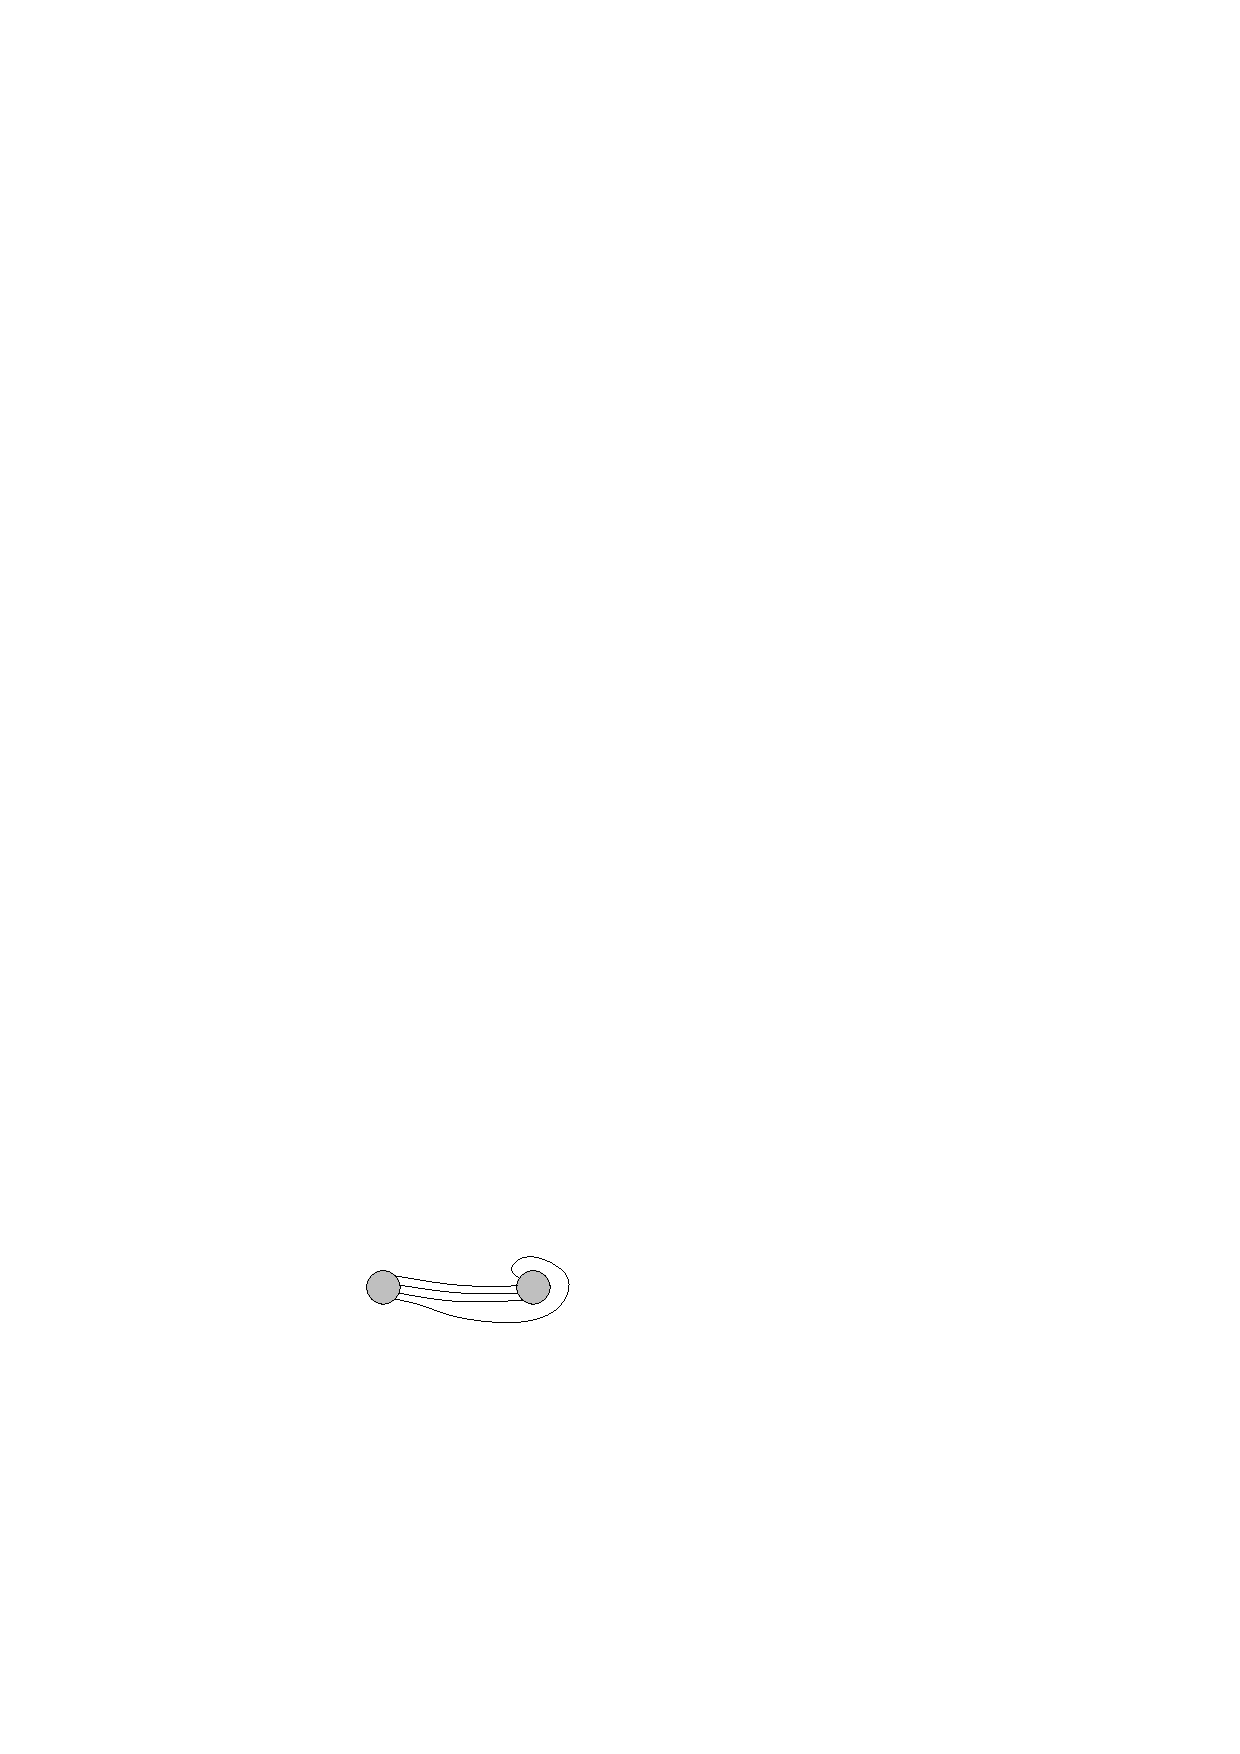
\includegraphics[scale=1.5]{graphics/hd-examples}
\caption{Heegaard diagram for $L(4,1)$}
\label{hd-examples}
\end{figure}

\begin{example}
Let us figure out the Heegaard diagram for the 3-torus $T^3 = S^1 \times S^1 \times S^1$. We do this by remembering how the product of a $k$- and $l$-handle become a $(k+l)$-handle. 
\end{example}







\subsection{Kirby Diagrams}
\label{Kirby Diagrams}


A \textbf{Kirby diagram} is a diagram we can associate to a 4-dimensional handlebody $X$. We start with a 4-ball $D^4$, and think of its boundary $\partial D^4 = S^3$ as $\mathbb R^3 \cup \lcb \infty \rcb$. We attach 1-handles to this via an embedding of $D^3 \sqcup D^3$. There is the issue of framing (there are two framings), but for now let us choose the framing such that $X_1 = \natural m S^1 \times D^3$ (here we are attaching $m$ 1-handles). We can represent this in $\mathbb R^3 \cup \lcb \infty\rcb$ by drawing $2m$ disjoint embedded 3-balls in $\mathbb R^3 \cup\lcb\infty\rcb$ and pairing them so that when we identify pairs in an orientation reversing manner we get $X_1 = \natural m S^1 \times D^3$. 

To attaching a 2-handle to $X_1$ we specify a knot in $X_1$ (the attaching circle) and label it with a framing. So, a diagram of $X_2$ consists of $m$ pairs of 3-balls and a collection of arcs that either start and end on the boundary of the 3-balls, or form a closed loop. We can specify a framing on a knot component by a nowhere zero normal vector field, or equivalently, a parallel knot. Once we specify which parallel corresponds to $0 \in \pi_1(O(2))=\mathbb Z$ we can get any other framing by adding full left or right twists. We will choose the parallel which has linking number 0 with the knot to be the framing corresponding to $0$. 

It turns out that there is essentially a unique way to attach 3-handles and 4-handles so that we obtain a closed manifold, so our diagram of $X$ can stop here. Things are more complicated when $\partial X \neq \emptyset$, but we will not deal with that now.



\todo{need more on this...}



\begin{example}
Let us find a Kirby diagram of $S^2 \times S^2$. The 2-sphere has the obvious decomposition $S^2 = D_- \cup D_+$, where $D_-$ is a 0-handle, $D_+$ a 2-handle, which we think of as the southern and northern hemispheres. The attaching map for the 2-handle is just the identity. The handlebody decomposition of $S^2 \times S^2$ is just
\[ S^2 \times S^2 = \overbrace{D_- \times D_-}^{0-\text{handle}} \cup \overbrace{D_+ \times D_-}^{2-\text{handle}} \cup \overbrace{D_- \times D_+}^{2-\text{handle}} \cup \overbrace{D_+ \times D_+}^{4-\text{handle}} \]
First we determine the attaching maps for the 2-handles. One is the map $\varphi_1 : \partial D_+ \times D_- \rightarrow \partial(D_- \times D_-)$ defined by $\varphi_1(x,y)=(x,y)$, and the other is the map $\varphi_2 : \partial D_- \times D_+ \rightarrow \partial(D_-\times D_-)$ is defined by $\varphi_2(x,y)=(y,x)$. Clearly the attaching regions of these maps is the Hopf link in $S^3$ and their framings are zero. Therefore \cref{kirby-diagram-s2xs2} is a Kirby diagram for the 4-manifold $S^2 \times S^2$.

\begin{figure}[tb]
\centering

\includegraphics[scale=1]{graphics/kirby-diagram-s2xs2}
\caption{Kirby Diagram of $S^2 \times S^2$}
\label{kirby-diagram-s2xs2}
\end{figure}
\end{example}

\begin{example}
Let us find a handlebody decomposition of $S^2 \tilde\times S^2$. Recall that this is the boundary of the non-trivial $D^3$ bundle over $S^2$.

\begin{figure}[tb]
\centering

\includegraphics[scale=1]{graphics/kirby-diagram-twisted-s2xs2}
\caption{Kirby Diagram of $S^2 \tilde\times S^2$}
\label{kirby-diagram-twisted-s2xs2}
\end{figure}
\end{example}



\begin{example}
Let us figure out the Kirby diagrams for orientable 4-manifolds $X$ arising as $D^2$-bundles $\pi : X \rightarrow F$ over a closed surface. To begin with, let us assume that $F$ is connected and orientable of genus $g$.... \unfinished
\end{example}












\newpage
\section{Morse Theory}
\label{Morse Theory}



\subsection{Morse Functions}
\label{Morse Functions}



We start with a smooth $n$-manifold $M$ and a smooth function $f : M \rightarrow \mathbb R$. Take a chart $(x,U)$, that is an open set $U \subset M$ and a homeomorphism $x : U \rightarrow \mathbb R^n$. If we write $x$ in components $x = (x^1,\ldots,x^n)$, then we define the derivative of $f$ at some point $p \in U$ with respect to this chart by
\[ \pfrac{f}{x^i}(p) = D_i (f \circ x^{-1})(x(p)) \]
where $D_i$ is the regular derivative of $f \circ x^{-1} : \mathbb R^n \rightarrow \mathbb R$ in the $i$-th component. Recall that if $(y,V)$ is another chart, then the derivative of $f$ with respect to these two charts on the overlap are related by
\begin{equation}
\label{derivative transformation rule}
\pfrac{f}{y^i} = \sum_{j=1}^n \pfrac{f}{x^j} \pfrac{x^j}{y^i}
\end{equation}
Another way of saying this is to first define the \textbf{Jacobian} matrix of two charts $(x,U)$ and $(y,V)$. This is the matrix whose $(i,j)$-entry is equal to $\pfrac{x^i}{y^j}$, and it is denoted by $J_y^x$. If we let $\pfrac{f}{x}$ denote the column vector of derivatives of $f$, then \eqref{derivative transformation rule} simply says
\[ \pfrac{f}{y} = J_y^x \cdot \pfrac{f}{x} \]
Since $\pfrac{f}{x^i}$ is just another smooth map from $U$ to $\mathbb R$ we can take a second derivative with respect to a chart. The second derivatives calculated with respect to different charts are related by
\begin{equation}
\label{second derivative transformation rule}
\pfrac{^2 f}{y^i \partial y^j} = \pfrac{^2 f}{x^k \partial x^\ell} \pfrac{x^k}{y^i} \pfrac{x^\ell}{y^j}
\end{equation}
As with first derivatives there is another way of looking at this. Let us define the \textbf{Hessian} of $f$ with respect to the chart $x$ be the matrix whose $(i,j)$-entry is $\pfrac{^2 f}{x^i \partial x^j}$, and it is denoted by $H_f^x$. Since partial derivatives commute we have that $H_f^x$ is symmetric. We now see that \eqref{second derivative transformation rule} can be written as
\begin{equation}
\label{second derivative matrix transformation rule}
H_f^y = (J_y^x)^t \cdot H_f^x \cdot J_y^x
\end{equation}
This tells us that even though the Hessian as a matrix is not well-defined (i.e. it depends on the chart), it is well-defined as a bilinear form. There is also a nice coordinate free way of describing the Hessian. Let $\nabla : \Gamma(TM) \times \Gamma(T^*M) \rightarrow \Gamma(T^*M)$ be any connection on $T^*M$, and for any $p \in M$ define the map $H_f(p) : T_p M \rightarrow T_p^* M$ by
\begin{equation}
\label{connection definition of Hessian}
H_f(p)(X) = \nabla_X (df)
\end{equation}
This does not depend on the choice of connection, for if $\widetilde\nabla$ is another connection, then the difference $\nabla-\widetilde\nabla$ is tensorial in both arguments and $df_p=0$, hence $\nabla_X(df)-\widetilde\nabla_X(df)=0$ at $p$.

Suppose that a point $p \in M$ is a critical point of $f$, i.e. $df_p=0$. We say that $p$ is a \textbf{non-degenerate} critical point if $\det H_f^x(p)$ is nonzero for some chart $x$, hence every chart by \eqref{second derivative matrix transformation rule}. We define the \textbf{index} of a critical point $p$ to be the number of negative eigenvalues of the Hessian at $p$, which is well-defined by \eqref{second derivative matrix transformation rule}, and is denoted by $\mu(p)$. Equivalently, we call the critical point $p$ non-degenerate if $H_f(p)$ does not have 0 for an eigenvalue, and $\mu(p)$ is the number of negative eigenvalues of $H_f(p)$. Finally, we define a \textbf{Morse function} is a smooth function with all non-degenerate critical points. 

It turns out that Morse functions look very nice around critical points. The Morse lemma gives a precise statement of this, and will be very important in our discussion of cell decompositions of spaces via Morse functions. First we recall a basic fact from calculus using the fundamental theorem.

\begin{lem}
\label{FTC cor}
Let $U$ be a convex subset of $\mathbb R^n$ containing 0 and $f : U \rightarrow \mathbb R$ a smooth function with $f(0) = 0$. Then we can write
\[ f(x_1,\ldots,x_n) = \sum_{i=1}^n x_i g_i(x_1,\ldots,x_n) \]
for some $g_i : U \rightarrow \mathbb R$ with $g_i(0) = \pfrac{f}{x_i}(0)$.
\end{lem}
\begin{proof}
For fixed $x_1,\ldots,x_n$ we apply the fundamental theorem of calculus and chain rule to get
\[ f(x_1,\ldots,x_n) = \int_0^1 \frac{df(tx_1,\ldots,tx_n)}{dt} \, dt = \int_0^1 \sum_{i=1}^n x_i \cdot \pfrac{f}{x_i}(tx_1,\ldots,tx_n) \, dt \]
So let $g_i(x_1,\ldots,x_n) = \int_0^1 \pfrac{f}{x_i}(tx_1,\ldots,tx_n) \, dt$, then clearly $g_i(0) = \pfrac{f}{x_i}(0)$ and we are done.
\end{proof}


\begin{lem}[Morse Lemma]
\label{Morse Lemma}
Let $f : M \rightarrow \mathbb R$ be a smooth function and $p \in M$ a non-degenerate critical point. Then there is a chart $y = (y^1,\ldots,y^n)$ on a neighborhood $U$ of $p$ such that $y^i(p) = 0$ and
\[ f = f(p) - (y^1)^2 - \cdots - (y^\mu)^2 + (y^{\mu+1})^2 + \cdots + (y^n)^2 \]
on $U$, where $\mu$ is the index of $p$.
\end{lem}
\begin{proof}
First note that finding a chart so that $f$ can be expressed in the above form is equivalent to finding a chart $(x,U)$ such that on $U$ we have
\[ (f \circ x^{-1})(t_1,\ldots,t_n) = -t_1^2 - \cdots - t_\mu^2 + t_{\mu+1}^2 + \cdots t_n^2 \]
where $t_i$ are real numbers. Therefore we can, without loss of generality, assume that $f$ is defined on some open set $V$ of $\mathbb R^n$ (say containing zero), and by performing some translations we can assume $p=0$ and $f(0)=0$.

Next it is clear that if $f$ can be represented in the above form for some chart $(y,U)$, then we have
\[ \pfrac{^2 f}{y^i \partial y^j}(p) = \begin{cases} -2 & i=j, j \leq \mu \\ 2 & i=j, j > \mu \end{cases} \]
Therefore the Hessian $H_f^x$ is already diagonalized in this coordinate system, and clearly has $\mu$ negative entries along the diagonal. Therefore $\mu$ really will be the index of $p$ if we can get $f$ into the above form.

Let $x=(x^1,\ldots,x^n)$ be the standard coordinates on $\mathbb R^n$. By \cref{FTC cor} we can find functions $g_i : V \rightarrow \mathbb R$ such that
\[ f(x^1,\ldots,x^n) = \sum_{i=1}^n x^i \cdot g_i(x^1,\ldots,x^n) \]
and $g_i(0) = \pfrac{f}{x^i}(0)$. However, since $p=0$ is assumed to be a critical point we have $\pfrac{f}{x^i}(0) = 0$, so we can apply \cref{FTC cor} to the functions $g_i$ to obtain functions $h_{ij} : V \rightarrow \mathbb R$ such that
\[ g_i(x^1,\ldots,x^n) = \sum_{j=1}^n x^j h_{ij}(x^1,\ldots,x^n) \]
and $h_{ij}(0) = \pfrac{g_i}{x^j}(0) = \pfrac{^2 f}{x^i \partial x^j}(0)$. Combining the above two expressions yields
\begin{equation}
\label{quadratic form of f}
f(x^1,\ldots,x^n) = \sum_{i,j=1}^n x^i x^j h_{ij} (x^1,\ldots,x^n)
\end{equation}
If we define $\widetilde{h}_{ij} = \frac{1}{2}(h_{ij} + h_{ji})$, then we see that $\widetilde{h}_{ij} = \widetilde{h}_{ji}$ and yet still $f = \sum x^i x^j\widetilde{h}_{ij}$. Therefore we can assume that $h_{ij} = h_{ji}$. It is also clear that the matrix $(h_{ij}(0))_{ij}$ is equal to $\frac{1}{2} H_f^x$. 

We now simply mimic the proof of the diagonalization of quadratic forms, applied to $(h_{ij})$, to show that we can find coordinates to bring $f$ into the desired form. By assumption the Hessian is non-singular, so $(h_{ij}(0))$ is also non-singular. Reordering the coordinate system can assume that $h_{11}(0) \neq 0$, and so by continuity we have that $h_{11}(0) \neq 0$ on some small neighborhood $V'$ of $0$. Let us also assume that $h_{11} > 0$ on $V'$ (the other case is treated similarly). We introduce a new coordinate $y^1 : V' \rightarrow \mathbb R$ defined by
\begin{equation}
\label{new coordinate}
y^1 = \sqrt{h_{11}} \left( x^1 + \sum_{i=2}^n \frac{x^i h_{1i}}{h_{11}} \right)
\end{equation}
The coordinates $(y^1,x^2,\ldots,x^n)$ form a chart (in a possibly smaller neighborhood $V''$ of $0$). Squaring this new coordinate gives
\begin{equation}
\label{square of new coordinate}
\begin{array}{rl}
	(y^1)^2 &= \displaystyle h_{11} \left( x^1 + \sum_{i=2}^n \frac{x^i h_{1i}}{h_{11}} \right)^2 \\
	        &= \displaystyle h_{11} \left( (x^1)^2 + 2 \sum_{i=2}^n \frac{x^1 x^i h_{1i}}{h_{11}} + \left( \sum_{i=2}^n \frac{x^i h_{1i}}{h_{11}} \right)^2 \right) \\
	        & \\
	        &= \displaystyle h_{11} (x^1)^2 + 2 \sum_{i=2}^n x^1 x^i h_{1i} + \frac{1}{h_{11}} \left( \sum_{i=2}^n x^i h_{1i} \right)^2 
\end{array}
\end{equation}
This expression allows us to rewrite $(x^1)^2$ as
\begin{equation}
\label{rewrite of (x^1)^2}
h_{11} (x^1)^2 = (y^1)^2 - 2 \sum_{i=2}^n x^1 x^i h_{1i} - \frac{1}{h_{11}} \left( \sum_{i=2}^n x^i h_{1i} \right)^2 
\end{equation}
Now, using \eqref{quadratic form of f} and \eqref{rewrite of (x^1)^2} we can rewrite $f$ in coordinates $(y^1,x^2,\ldots,x^n)$ as
\begin{align*}
	f &= h_{11} (x^1)^2 + 2 \sum_{i=2}^n x^1 x^i h_{1i} + \sum_{i,j=2}^n x^i x^j h_{ij} \\
	  &= (y^1)^2 - 2 \sum_{i=2}^n x^1 x^i h_{1i} - \frac{1}{h_{11}} \left( \sum_{i=2}^n x^i h_{1i} \right)^2 + 2 \sum_{i=2}^n x^1 x^i h_{1i} + \sum_{i,j=2}^n x^i x^j h_{ij} \\
	  &= (y^1)^2 + \sum_{i,j=2}^n x^i x^j h_{ij} - \frac{1}{h_{11}} \left( \sum_{i=2}^n x^i h_{1i} \right)^2 \\
\end{align*}
Note that had we assumed $h_{11} < 0$ on $V'$, then we would have $-(y^1)^2$ in the above. The terms in this last expression only involve $x^i$'s for $i \geq 2$, so we can repeat the above arguments to find a new coordinate $y^2$ such that $(y^1,y^2,x^3,\ldots,x^n)$ is a coordinate system and
\[ f = \pm (y^1)^2 \pm (y^2)^2 \pm \text{ terms with } x^3, x^4, \ldots, x^n \]
Continuing this we get a coordinate system $y=(y^1,\ldots,y^n)$ such that
\[ f = \pm (y^1)^2 \pm  \cdots + (y^n)^2 \]
Since the number of minus signs is equal to $\mu$, which does not depend on coordinate charts, we are done.
\end{proof}

A simple consequence of the Morse lemma is the following.

\begin{cor}
The critical points of a Morse function are isolated.
\end{cor}





\subsection{Handlebody Decompositions Induced by Morse Functions}
\label{Handlebody Decompositions Induced by Morse Functions}


For a manifold $M$ with Morse function $f : M \rightarrow \mathbb R$, let us define the sets $M^a = f^{-1}(-\infty,a]$. If $a$ is not a critical value, then $M^a$ is a submanifold with boundary. We will now analyze what happens to $M^a$ as $a$ crosses a critical value. Our first theorem towards this says that the diffeomorphism type of $M^a$ does not change between critical values. First let us develop the notion of gradient vector fields and flows.

Let $(M,g)$ be a Riemannian manifold with Morse function $f : M \rightarrow \mathbb R$. Recall that the metric gives us a canonical isomorphism of tangent spaces with cotangent spaces by mapping a vector $X \in T_p M$ to the covector $g(X,-) \in T_p^* M$. The gradient vector field of $f$ is the unique vector field $\nabla_g f$ corresponding to the 1-form $df$ under this isomorphism, hence
\[ g(X,\nabla_g f) = df(X) \]
for any vector field $X$. In coordinates $(x^1,\ldots,x^n)$ we can write
\[ \nabla_g f = \sum_{i,j = 2}^n g^{ij} \pfrac{f}{x^j} \pfrac{}{x^i} \]
where $g^{ij}$ are the components of the inverse metric. It is clear that $\nabla_g f$ vanishes at precisely the critical points of $f$. 

\begin{thm}
Let $[a,b]$ be an interval that does not contain any critical values and such that $f^{-1}[a,b]$ is compact. Then $M^a$ is diffeomorphic to $M^b$. In fact, $M^a$ is a deformation retract of $M^b$.
\end{thm}
\begin{proof}
First note that the compactness hypothesis would be immediate if we assumed that $M$ is compact. Let $X$ be a vector field given by
\[ X = \frac{\nabla_g f}{\norm{\nabla_g f}^2} \]
on $f^{-1}[a,b]$, and vanish identically outside some compact set containing $f^{-1}[a,b]$. Since this vector field has compact support it generates a unique 1-parameter group $\phi_t : M \rightarrow M$ of diffeomorphisms. For fixed $p \in M$ such that $\phi_t(p)$ lies in $f^{-1}[a,b]$, the function $f \circ \phi(p)$ is a map $\mathbb R \rightarrow \mathbb R$, and we can compute (using the chain rule and definition of $\nabla_g f$)
\[ \frac{d f(\phi_t(p))}{dt} = df(d\phi_t(d/dt)) = g(d\phi_t(d/dt),\nabla_g f) = \frac{g(\nabla_g f,\nabla_g f)}{g(\nabla_g f,\nabla_g f)} = 1 \]
So, the function $f \circ \phi(p) : \mathbb R \rightarrow R$ is linear; in fact, $f(\phi_t(p)) = t + f(\phi_0(p)) = t+f(p)$. So, if we take a point $p$ with $f(p) = a$, then $f(\phi_{b-a}(p)) = (b-a)+a=b$, hence $\phi_{b-a}$ maps $M^a$ into $M^b$. Similarly, $\phi_{b-a}^{-1} = \phi_{a-b}$ maps $M^b$ into $M^a$, hence $M^b$ is diffeomorphic to $M^a$, and this proves the first part of the theorem.

For the second part of the theorem we can construct the deformation retract explicitly. Consider the homotopy $r_t : M^b \rightarrow M^b$ defined by
\[ r_t(x) = \begin{cases} x & f(x) \leq a \\ \phi_{t(a-f(x))} (x) & a \leq f(x) \leq b \end{cases} \]
We clearly have $r_0 = \id$ and $r_1$ is a retract of $M^b$ onto $M^a$, therefore $M^a$ is a deformation retract of $M^b$.
\end{proof}

\begin{thm}
\label{Morse handle attachment}
Let $f : M^n \rightarrow \mathbb R$ be a smooth function with a non-degenerate critical point $p$ of index $\mu$. Let $c=f(p)$ and suppose $f^{-1}[c-\varepsilon,c+\varepsilon]$ is compact, and contains no critical points of $f$ other than $p$. Then for small enough $\varepsilon$, the manifold $M^{c+\varepsilon}$ is diffeomorphic to $M^{c-\varepsilon}$ with an $n$-dimensional $\mu$-handle attached.
\end{thm}
\begin{proof}
See \cref{around-a-critical-point} for the local behavior of $f$ around the critical point $p$. Take a chart $(x,U)$ around $p$ as in the Morse lemma. Then the lightly shaded region is the set of points $(x^1,\ldots,x^n)$ with $f(x^1,\ldots,x^n) \leq c-\varepsilon$, and the medium shaded region is the set of points with $c-\varepsilon \leq f(x^1,\ldots,x^n) \leq c+\varepsilon$. The intersection of the medium shaded region with the $(x^1,\ldots,x^\mu)$-axis is the set of points $(x^1,\ldots,x^\mu)$ with $(x^1)^2 + \cdots (x^\mu)^2 \leq \varepsilon$, hence a $\mu$-dimensional ball. The intersection of the medium shaded region with the $(x^{\mu+1},\ldots,x^n)$-axis is the set of points $(x^{\mu+1},\ldots,x^n)$ with $(x^{\mu+1})^2 + \cdots + (x^n)^2 \leq \varepsilon$, hence a $(n-\mu)$-dimensional ball.

The dark region $h$ in the figure consists of the set of points $(x^1,\ldots,x^n)$ such that 
\[ (x^1)^2 + \cdots + (x^\mu)^2 - (x^{\mu+1})^2 - \cdots - (x^n)^2 \leq \varepsilon \ \ \ \text{and} \ \ \ (x^{\mu+1})^2 + \cdots + (x^n)^2 \leq \delta \]
for sufficiently small $\delta$. Clearly this region is diffeomorphic to $D^\mu \times D^{n-\mu}$, and intersects $M^{c-\epsilon}$ at the points $\partial D^\mu \times D^{n-\mu}$, i.e. 
\[ (x^1)^2 + \cdots + (x^\mu)^2 - (x^{\mu+1})^2 - \cdots - (x^n)^2 = \varepsilon \ \ \ \text{and} \ \ \ (x^{\mu+1})^2 + \cdots + (x^n)^2 \leq \delta \]
One can now use the gradient flow of $f$ to show that $M^{c+\epsilon}$ is diffeomorphic to $M^{c-\epsilon} \cup h$, hence a $\mu$-handle was attached.

\begin{figure}[tb]
\centering
\ \ \ \ \ \ \ \ \ \ \ \ \ \ \ \ \ \ \ 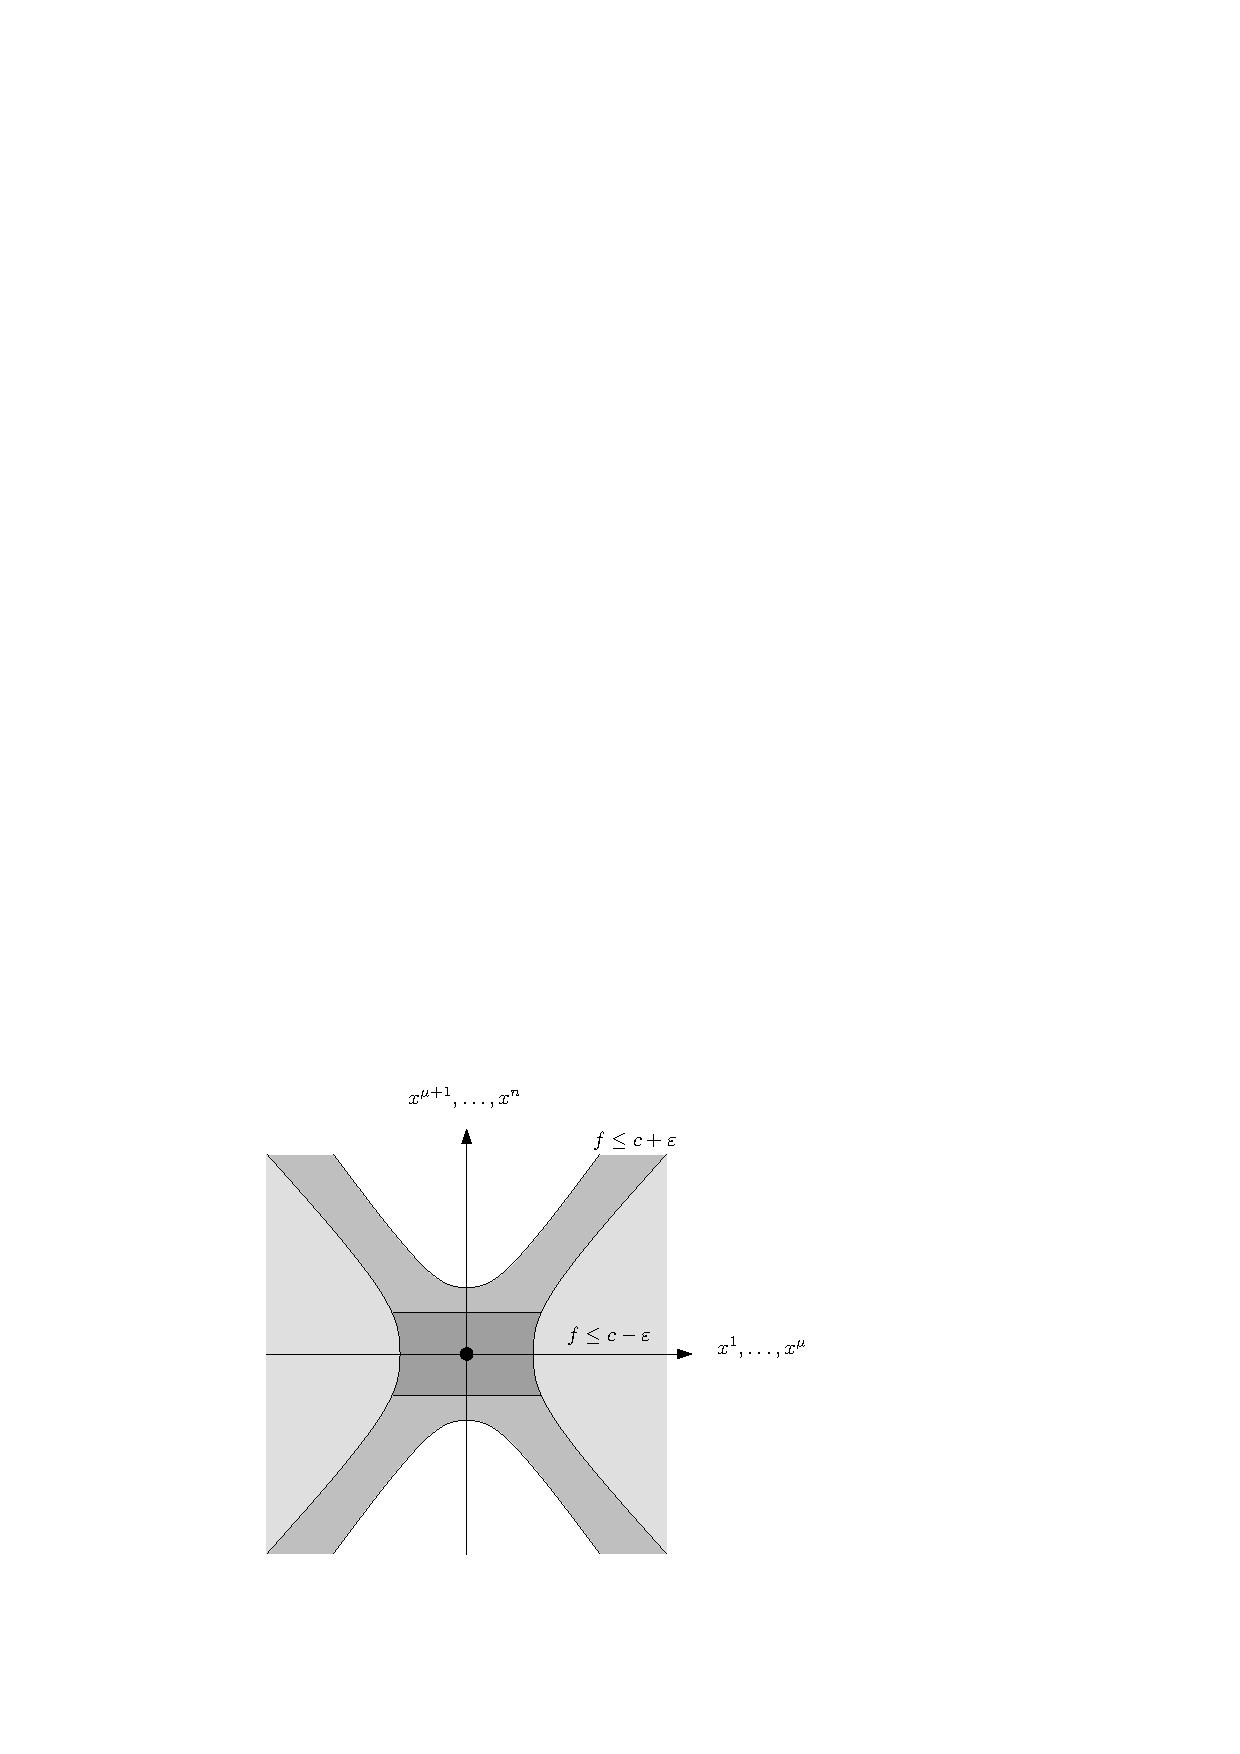
\includegraphics[scale=1]{graphics/around-a-critical-point}
\caption{Behavior of $f$ around a critical point}
\label{around-a-critical-point}
\end{figure}
\end{proof}

\Cref{Morse handle attachment} and \cref{around-a-critical-point} also give an explicit description of the attaching spheres of the handle attached. If the handle $h$ is attached to $M^{c-\varepsilon}$ to obtain $M^{c+\varepsilon}$, then the attaching sphere of $h$ is precisely where the descending manifold of $p$ intersects the boundary of $M^{c-\varepsilon}$.



\begin{thm}
\label{Morse handle decomposition}
If $f$ is a Morse function on a manifold $M$, and if each $M^a$ is compact, then $M$ has a handlebody decomposition with one $\mu$-handle for each critical point of index $\mu$.
\end{thm}



\subsection{Properties of Gradient Flows}
\label{Properties of Gradient Flows}


Let us further investigate the properties of flows of gradient vector fields. For this section all of our manifolds will be closed.
\begin{prop}
\label{decrease along negative gradient flow line}
Every function decreases along its negative gradient flow lines.
\end{prop}
\begin{proof}
Let $f : M \rightarrow \mathbb R$ be $C^1$ and $u : \mathbb R \rightarrow M$ a flow line of $-\nabla_g f$. Since $f \circ u$ is $C^1$ we have, by the fundamental theorem of calculus, that for any $b>a$
\begin{align*}
	f(u(a))-f(u(b)) &= \int_b^a \frac{d}{dt} f \circ u(t) \, dt \\
	                &= -\int_a^b df_{u(t)} (du/dt) \, dt \\
	                &= -\int_a^b df_{u(t)} (-\nabla_g f(u(t))) \, dt \\
	                &= -\int_a^b g(\nabla_g f(u(t)),-\nabla_g f(u(t))) \, dt \\
	                &= \int_a^b \norm{\nabla_g f(u(t))} \, dt \\
	                &\geq 0
\end{align*}
Therefore $f(u(a)) \geq f(u(b))$, and so $f$ decreased along $u$.
\end{proof}

\begin{prop}
Letting $u$ be a flow line of $f$, if $u(\infty)=p$ or $u(-\infty)=p$, then $p$ is a critical point of $f$.
\end{prop}
\begin{proof}
First suppose $u(\infty)=p$ (the other case is similar). We have
\[ \lim_{t \to \infty} \int_0^t \norm{du/dt(s)}^2 \, ds = \lim_{t \to \infty} (f(u(0)) - f(u(t))) = f(u(0)) - f(p) < \infty \]
This forces $\norm{du/dt(t)} \to 0$ as $t \to \infty$. Therefore
\[ \norm{\nabla_g f(p)} = \lim_{t \to \infty} \norm{du/dt(t)} = 0 \]
and so $p$ is a critical point of $f$.
\end{proof}

\begin{prop}
If $p$ is a non-degenerate critical point of $f$, and $u$ is a negative gradient flow line with $u(\infty)=p$, then there are constants $C>0, \epsilon>0$ and $T >> 0$ such that
\[ d(u(t),p) \leq Ce^{-\epsilon t} \]
for all $t \geq T$.
\end{prop}





\subsection{Existence of Morse Functions}
\label{Existence of Morse functions}

We have proved quite a bit concerning Morse functions, but we have not yet shown that they always exist. It turns out that not only do they exist, but in some sense, almost all smooth functions satisfy the Morse property. We will prove this result and show that Morse functions can be chosen with special properties, such as with ``separated'' critical points and self-indexing critical points.

Since most theorems that involve the phrase ``almost every'' invoke Sard's theorem in some way, we begin with this result. Recall that a smooth function $f : M \rightarrow N$ is said to have a \textbf{critical point} at $p \in M$ if $\rank f_{*p} < \dim N$, and a point $q \in N$ is said to be a \textbf{critical value} of $f$ if $q=f(p)$ for some critical point $p \in M$.

\begin{thm}[Sard's Theorem]
\label{Sard's Theorem}
Let $f : \mathbb R^n \rightarrow \mathbb R^m$ be a smooth function. The critical values of $f$ have Lebesgue measure zero in $\mathbb R^m$.
\end{thm}

Sard's theorem gives us an easy proof that Morse functions are numerous on open sets of $\mathbb R^n$.

\begin{prop}
\label{existence of Morse functions on R^n}
Let $f : U \rightarrow \mathbb R$ be a smooth function on an open set $U \subseteq \mathbb R^n$. Then there exists numbers $a_1,\ldots,a_n$ such that 
\[ \widetilde f(x^1,\ldots,x^n) = f(x^1,\ldots,x^n) - a_1x^1 - \cdots - a_nx^n \]
has all non-degenerate critical points. Further, the $a_i$'s can be chosen arbitrary small.
\end{prop}
\begin{proof}
Define a function $h : U \rightarrow \mathbb R^n$ by
\[ h = \begin{pmatrix} h_1 \\ \vdots \\ h_n \end{pmatrix} = \begin{pmatrix} \pfrac{f}{x^1} \\ \vdots \\ \pfrac{f}{x^n} \end{pmatrix} \]
Then the Jacobian of $h$ is 
\[ J_h = \left( \pfrac{h_i}{x^j} \right) = \left( \pfrac{^2 f}{x^i \partial x^j} \right) \]
which is just the Hessian $H_f$ of $f$. So, the critical points of $h$ are precisely where $\det H_f = 0$. By \cref{Sard's Theorem} we can find a point $a = (a_1,\ldots,a_n) \in \mathbb R^n$ that is not a critical value of $h$. In fact, there are many such points, and we can choose this point as close to 0 as we want. For this point, define $\widetilde f : U \rightarrow \mathbb R$ by
\[ \widetilde f(x^1,\ldots,x^n) = f(x^1,\ldots,x^n) - a_1x^1- \cdots - a_nx^n \]
Let $p \in U$ be a critical point of $\widetilde f$, then
\[ 0 = \pfrac{\widetilde f}{x^i}(p) = \pfrac{f}{x^i}(p) - a_i \]
hence $h(p) = a$. Since $a$ is not a critical value of $h$ we have that $p$ is not a critical point of $h$, and so $\det H_f \neq 0$. Since $f$ and $\widetilde f$ differ only by a linear function we have that their Hessians are equal, so $\det H_{\widetilde f} = \det H_f \neq 0$, hence $p$ is a non-degenerate critical point of $\widetilde f$.
\end{proof}

We can use this proposition to prove the more general result
\begin{thm}
\label{existence of Morse functions on manifolds}
There exists a Morse function on any closed manifold $M$.
\end{thm}
\begin{proof}
Start with any smooth function $f_0 : M \rightarrow \mathbb R$. We will make a sequence of small changes to this function to remove degenerate critical points over open sets.

Let $\lcb U_i \rcb$ be a finite open cover of $M$ by charts, and let $\varphi_i : U_i \rightarrow \mathbb R$ be a collection of bump functions for $\lcb U_i \rcb$. Recall that this means that there is a compact set $K_i \subset U_i$ such that $\varphi_i \equiv 1$ on $K_i$, $0 \leq \varphi \leq 1$ on $U_i$ and $\varphi_i \equiv 0$ outside $U_i$. Without loss of generality we can assume that $\lcb K_i \rcb$ covers $M$. Let $\mathcal K_m = K_1 \cup \cdots \cup K_m$ and set $K_0 = \emptyset$. 

We will use an induction argument to remove degenerate critical points from $\mathcal K_m$. Clearly $f_0$ has no degenerate critical points in $\mathcal K_0$, so let us assume that $f_{m-1}$ has been constructed with no degenerate critical points in $\mathcal K_{m-1}$. Let $x : U_m \rightarrow \mathbb R^n$ be a chart for $U_m$, then $f_{m-1} \circ x^{-1} : x(U_m) \rightarrow \mathbb R$ is a function defined on an open set of $\mathbb R^n$. By \cref{existence of Morse functions on R^n} we can find small vector $a=(a_1,\ldots,a_n)$ such that
\[ f_{m-1} \circ x^{-1}(x^1,\ldots,x^n) - a_1x^1 - \cdots - a_nx^n \]
has only non-degenerate critical points. We can extend this function to all of $M$ by multiplying by the bump function, so we define
\[ f_m(p) = \begin{cases} f_{m-1}(p) - a \cdot x(p) \varphi_m(p) & p \in U_m \\ f_{m-1}(p) & p \notin \supp \varphi_m \end{cases} \]
This is a well-defined smooth function on $M$ since $\varphi_m \equiv 0$ on the overlap of $U_m$ and the complement of $\supp \varphi_m$. Now $f_m$ does not have any degenerate critical points on $K_m$, and since $f_{m-1}$ did not have any degenerate critical points on $\mathcal K_{m-1}$ it follows that $f_m$ is a Morse function on $\mathcal K_m$. This completes the proof by induction.
\end{proof}

The proof of \cref{existence of Morse functions on manifolds} actually shows a little more. Since we could pick the numbers $a_1,\ldots,a_n$ very small at each stage we could actually show that the constructed Morse function is $C^2$-close to the initial function $f_0$, hence there is a Morse function close to any smooth function.


\note{Other theorems to prove}

\begin{thm}
\label{existence of self-indexing Morse functions}
There is a Morse function $f : M \rightarrow \mathbb R$ on any closed manifold $M$ such that if $p,q \in M$ are critical points, then $f(p) \leq f(q)$ if and only if $\mu(p) \leq \mu(q)$.
\end{thm}

Such Morse functions are called \textbf{self-indexing}, and clearly the image of $M$ under $f$ is precisely $[0,n]$, where $n$ is the dimension of the manifold. 









\newpage
\section{Kirby Calculus}
\label{Kirby Calculus}




\subsection{Surgery on Links}
\label{Surgery on Links}


We have seen that Heegaard diagrams provide a nice combinatorial picture for 3-manifolds, even if they are a little unwieldy to work with. This is mostly due to the fact that self-homeomorphisms of high genus surfaces are difficult to understand. We will now present another combinatorial method of constructing 3-manifolds, called surgery on links. It has the advantage that we now only need to understand self-homeomorphisms of the torus, but the disadvantage that we now need to understand links better.

Given a 3-manifold $M$, let $k$ be an embedded knot in $M$ and $N(k)$ a tubular neighborhood, which is homeomorphic to $D^2 \times S^1$. Surgery on this knot is the proccess of cutting out the tubular neighborhood and gluing it back in. Since $M \backslash N(k)$ has boundary homeomorphic to $S^1 \times S^1$ we can find a homeomorphism $\varphi : \partial(D^2 \times S^1) \rightarrow \partial (M \backslash N(k))$ and form the quotient space $M_{k,\varphi} = (M \backslash N(k)) \cup_\varphi (D^2 \times S^1)$, which we call the \textbf{Dehn surgery on $k$ via $\varphi$}, or simply \textbf{surgery on $k$} since we are not going to discuss more general surgeries. The construction generalizes to links by performing it on each link component. Every closed, orientable 3-manifold can be obtained by such a construction applied to $M=S^3$, as we will see later.

\begin{prop}
A surgery $M_{k,\varphi}$ is completely determined by the image of $\partial D^2 \times \lcb * \rcb$ under $\varphi$.
\end{prop}
\begin{proof}
The solid torus $D^2 \times S^1$ can be attached in two steps. Let $J$ be a small segment of $S^1$ containing $*$. Then we can start by attaching $D^2 \times J$ to $M \backslash N(k)$. This leaves $D^2 \times J^c$ to be attached along its boundary, which is just a 3-ball being attached along a 2-sphere. There is only one way to attach this piece since every orientation preserving homeomorphism of $S^2$ is isotopic to the identity.
\end{proof}

So now a surgery can be described by a knot $k$ and a curve on $\partial(M \backslash N(k))$, which is where the meridian will be mapped under the attaching map. We can come up with a more combinatorial description of this curve, or more specifically, closed curves on the torus. Let $\alpha$ and $\beta$ be the meridian and longitude of the torus $T^2 = S^1 \times S^1$ so that $\pi_1(T^2) = \mathbb Z \oplus \mathbb Z$ is generated by $[\alpha]$ and $[\beta]$. For $p,q$ integers let $\gamma = p\alpha + q\beta$ denote a curve in the homotopy class $p[\alpha] + q[\beta]$, i.e. $\gamma$ wraps $p$ times around the meridian and $q$ times around the longitude. We have the following characterization of these curves.

\begin{prop}
\sloppyspace
\begin{enumerate}
	\item If a curve $\gamma$ in the homotopy class $p[\alpha] + q[\beta]$ has no self-intersections, then either $p$ and $q$ are relatively prime, or one of them is 0 and the other $\pm 1$. 
	\item If two closed curves on the torus are homotopic and without self-intersections, then they are isotopic.
\end{enumerate}
\end{prop}

Therefore isotopy classes of curves on $T^2$ are in one-to-one correspondence with pairs of relatively prime integers.

Let us apply this to a knot $k$ in $S^3$. Let $\mu$ be a canonical meridian of $\partial N(k)$, and let $\ell$ be the canonical longitude of $\partial N(k)$. Recall that this means that $\lk(\ell,k)=0$. Choose orientations on $\mu$ and $\ell$ such that the ordered basis $(\mu,\ell,n)$ matches the orientation of $S^3$, where $n$ is the outward pointing normal to $\partial N(k)$. If we glue a solid torus $D^2 \times S^1$ into $S^3 \backslash N(k)$ via $\varphi : \partial D^2 \times S^1 \rightarrow \partial(M \backslash N(k))$, then we know $\varphi$ must map the meridian $\partial D^2 \times \lcb * \rcb$ to a curve $p\mu + q\ell$, for some relatively prime integers $p,q$ (or possibly one equal to 0 and the other $\pm 1$). Therefore a surgery can now be described simply by a knot and an extended rational number $p/q \in \mathbb Q \cup \lcb \infty \rcb$. This is also called \textbf{rational surgery}. If $q = \pm 1$, then the surgery is called an \textbf{integral surgery}. We call the rational number $p/q$ the \textbf{framing index} of $k$, or simply the \textbf{framing}. This discussion applies equally well to knots embedded in an integral homology sphere. 

Here is a simple proposition relating surgeries to Heegaard splittings, as well as a powerful corollary.

\begin{prop}
\label{Heegaard splitting and surgery relationship}
Let $f_1,f_2 : \partial H \rightarrow \partial H'$ be homeomorphisms of the surfaces of two handlebodies such that $f_1 = f_2 \circ \tau_c$, where $\tau_c$ is a Dehn twist along a simple closed curve $c$ in $\partial H$. Set $M_i = H \cup_{f_i} H'$ for $i=1,2$. Then $M_2$ is obtained from $M_1$ by an integral surgery along a knot $k \in M_1$ isotopic to $c$. 
\end{prop}
\begin{proof}
Let $k$ be a knot in $H$ obtained from pushing $c$ a little $H$. Connect a tubular neighborhood $N(k)$ of $k$ to $\partial H$ via an annulus $A \cong S^1 \times I$ such that $S^1 \times \lcb 0 \rcb$ corresponds to a longitude $k'$ on $\partial N(k)$ and $S^1 \times \lcb 1 \rcb$ corresponds to $c$. There is a self-homeomorphism $\varphi$ of $H \backslash N(k)$ that is the result of cutting $H \backslash N(k)$ along $A$, performing a full twist on one of the rims, and then gluing the rims back together. Clearly $\varphi$ is just an extension of $\tau_c$ to $H \backslash N(k)$, but also its restricted to the torus $\partial N(k)$ is a Dehn twist around $k'$. Let $M_i' = (H \backslash N(k)) \cup_{f_i} H'$, i.e. $M_i'$ is $M_i$ with a solid torus removed. Then $M_1'$ and $M_2'$ are homeomorphic via the map
\[ h(x) = \begin{cases} \varphi(x) & x \in H \backslash N(k) \\ x & x \in H' \end{cases} \]
The fact that $M_1$ and $M_2$ become homeomorphic after removing a solid torus means that $M_1$ is obtained from $M_2$ via a surgery on $k$. In particular, the meridian $\mu$ of $\partial N(k)$ is wrapped around $\mu+k'$, hence it is an integral surgery.
\end{proof}

\begin{thm}[Lickorish-Wallace]
\label{Lickorish-Wallace theorem}
Every closed, orientable 3-manifold $M$ can be obtained from an integral surgery on a link embedded in $S^3$.
\end{thm}
\begin{proof}
By \cref{existence of heegaard splitting} we know that $M = H \cup_{f_2} H'$, where $H,H'$ are handlebodies and $f_2$ is an orientation reversing homeomorphism of their boundaries. Similarly $S^3 = H \cup_{f_1} H'$. Then $f_2^{-1} \circ f_1$ is an orientation preserving homomeomorphism of a surface of genus $g$, hence by the Dehn-Lickorish theorem (\todo{do this theorem}) we have $f_1 = f_2 \circ \tau_{c_1} \circ \cdots \tau_{c_n}$, where $\tau_{c_i}$ is a Dehn twist around a simple, closed curve $c_i$. Therefore by \cref{Heegaard splitting and surgery relationship} we have that $M$ is a sequence of integral surgeries on knots in $S^3$, or equivalently an integral surgery on a link.
\end{proof}

A \textbf{surgery diagram} for $S^3$ is a link diagram with each component labeled with an element of $\mathbb Q \cup \lcb \infty \rcb$. The canonical longitude of a knot $k$ can be drawn in a diagram by just drawing a parallel copy of the knot next to $k$ such that its linking number with $k$ is 0. However, take note that the first Reidemeister move will change this canonical longitude, so one needs to be careful. We will now explain the subtleties of this situation.

Consider the case of integral surgeries on knots in $S^3$, so let $k$ be a knot with integral framing $n$. This framing uniquely determines (up to isotopy) a longitude $\ell$ of $k$ such that $\lk(k,\ell)$, which is the curve we glue the meridian to when we perform the surgery. What is the meaning of the Reidemeister moves in a surgery diagram? It is clear that performing $R_2$ and $R_3$ moves does not change the manifold resulting from performing surgery on the knot, so we will continue calling these moves $R_1$ and $R_2$ on surgery diagrams. However, performing an $R_1$ move makes the longitude wrap one more time around the knot. This is the so-called ``belt trick,'' and is shown in \cref{belt trick}. This means that the framing of the knot will need to change by $\pm 1$, depending on which way you twist. This move on surgery diagrams will be called $R_1'$ due to its equivalent interpretation as a Reidemeister move for ribbons, and is shown in \cref{ribbon reidemeister I}. The inverse of the first $R_1'$ is called adding a \emph{left twist}, and the inverse of the other $R_1'$ move is called adding a \emph{right twist}. Now two surgery diagrams related by a finite number of $R_1'$, $R_2$ and $R_3$ moves give homeomorphic manifolds, but does the converse hold? Unfortunately no, but there are two more moves one can add, called Kirby moves, for which the converse holds. This is discussed in \cref{Kirby Moves}.

\begin{figure}[tb]
\centering
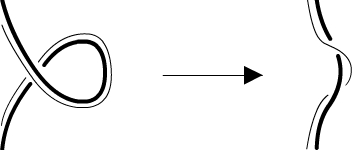
\includegraphics[scale=.6]{graphics/belt-trick}
\caption{Belt Trick}
\label{belt trick}
\end{figure}

\begin{figure}[tb]
\centering
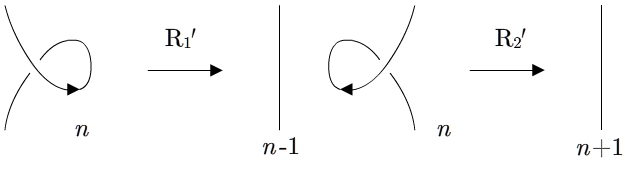
\includegraphics[scale=.6]{graphics/ribbon-reidemeister-I}
\caption{Ribbon Reidemeister I}
\label{ribbon reidemeister I}
\end{figure}

\begin{example}
The $1/0=\infty$ surgery on the unknot in $S^3$ results in $S^3$ again since we are just cutting out an unknotted, solid torus and gluing it back in the same way. Performing a 0-surgery on the unknot means to cut out an unknotted, solid torus $H$ from $S^3$ and glue it back in such that the meridian wraps once around the longitude. However, this longitude is precisely the meridian of the the solid torus $S^3 \backslash H$, so this surgery is really just gluing two solid tori together so that their meridians are identified, hence this is $S^1 \times S^2$. 

More generally, a surgery on the unknot in $S^3$ with surgery coefficient $-p/q$ ($p$ and $q$ relatively prime or one equal to 0 and the other 1) results in $L(p,q)$. This is because we cut out an unknotted, solid torus $H$ from $S^3$ and glue it back it so that the meridian wraps $p$ times around the longitude and $q$ times around the meridian. However, $H$'s meridian is precisely $S^3 \backslash H$'s longitude, and $H$'s longitude is precisely $S^3 \backslash H$'s meridian, hence we are just gluing together two solid tori so that the meridian of one gets wrapped $p$ times around the longitude and $q$ times around the meridian of the other torus. This is precisely the Heegaard splitting description of $L(p,q)$. Compare this with \cref{Heegaard splitting description of lens spaces}. We can also find a surgery diagram for $L(p,q)$ that has only integral surgery coefficients. See \cref{surgery-s1xs2-lpq}. 

\begin{figure}[tb]
\centering
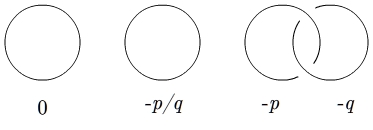
\includegraphics[scale=.6]{graphics/surgery-s1xs2-l(p,q)}
\caption{Surgery diagrams for $S^1 \times S^2$, $L(p,q)$ and $L(pq-1,q)$}
\label{surgery-s1xs2-lpq}
\end{figure}
\end{example}


Let $k_i$, $1 \leq i \leq n$, denote the components of a surgery diagram of some link, let $k_i$ be framed by $p_i/q_i$ and let $M$ be the 3-manifold resulting from performing this surgery. If we let $K = S^3 \backslash (N(k_1) \cup \cdots \cup N(k_n))$ be the knot complement, then $H_1(K) = \mathbb Z^n$ and is generated by the meridians $\lcb \mu_i \rcb$ of the link. When we glue in a solid torus $S^1 \times D^2$ so that $\lcb * \rcb \times \partial D^2$ is wrapped $p_i$ times around the meridian of $k_i$ and $q_i$ times around the longitude, when add a relation to $H_1(K)$. Namely, we add the relation $p_i\mu_i + q_i\lambda_i=0$, where $\lambda_i$ is the canonical longitude of $k_i$, since we are essentially filling this curve with a disc. The longitudes can be expressed as a relation in terms of the $\mu_i$'s. Since $\lk(k_i,\lambda_i)=0$ we have that $\lambda_i$ bounds a surface $F_i$ (i.e. a Seifert surface) in $S^3 \backslash N(k_i)$ (but not necessarily in $K$). Cut a small disc out of $F_i$ at each intersection point of a different component $k_j$ with $F_i$, and orient it positively if the intersection is positive and negatively if the intersection is negative. Since $k_j$ and $F_i$ intersect $\lk(k_i,k_j)$ times (counted with sign), we have $\lambda_i = \sum_{j \neq i} \lk(k_i,k_j) \mu_j$. We have proved the following.
\begin{prop}
\label{first homology of surgery}
For a surgery diagram with components $k_1,\ldots,k_n$ and framings $p_1/q_1,\ldots,p_n/q_n$, the first homology of this surgery is the free abelian group on $n$ generators modulo the relations $p_i\mu_i + q_i\sum_{i\neq j}\lk(k_i,k_j)\mu_j=0$. 
\end{prop}
\begin{cor}
\label{first homology of integral surgery}
For a surgery diagram with components $k_1,\ldots,k_n$ and integral framings $p_1,\ldots,p_n$, let $A$ be the linking matrix of this link with respect to any orientation. Then the first homology of this surgery is isomorphic to $\mathbb Z^n / \image A$.
\end{cor}
\begin{cor}
If the linking matrix $A$ has $\det A = \pm 1$, then the surgery is a homology sphere. In particular, a surgery on any knot with framing $\pm 1$ is a homology sphere.
\end{cor}





\subsection{Kirby Moves}
\label{Kirby Moves}


We now describe two basic moves that can be performed on surgery diagrams that do not change the resulting surgered manifold. If a link $L$ can be written as $L = L_1 \cup L_2$, where $L_1$ and $L_2$ are links that can be separated by a ball, then clearly a surgery on $L$ is diffeomorphic to the connected sum of the surgeries on each $L_1$ and $L_2$. So, if we add an unknotted, unlinked component to any link $L$ with framing $\pm 1$, surgery on this new link is the connected sum of the surgery on $L$ and the surgery on the unknot with framing $\pm 1$, which is just $S^3$, hence the manifold is unchanged. The addition or removal of an unknotted, unlinked component with framing $\pm 1$ from a surgery diagram is called the \textbf{first Kirby move} ($K_1$). 

Next, suppose our link $L$ is expressed as $L = k_1 \cup k_2$, where $k_1$ and $k_2$ are knots with framing $n_1$ and $n_2$, and are not necessarily unlinked. Let $\ell$ be a longitude of $k_2$ defining its framing (i.e. $\lk(k_2,\ell)=n_2$), and let $k_1'$ be the connected sum of $k_1$ with $\ell$ along a band disjoint from $L$ and $\ell$, and let $L' = k_1' \cup k_2$. We then give $k_1'$ the framing $n_1+n_2+2\lk(k_1,k_2)$, where the linking number is computed with respect to the orientations on $k_1$ and $k_2$ that induce an orientation on $k_1'$ (there are only two, and both have the same linking number). Then surgery on $L$ gives the same manifold as surgery on $L'$, but we will wait to show this until later. This process of ``adding'' the component $k_1$ to $k_2$, sometimes also called ``sliding'' $k_1$ across $k_2$, is the \textbf{second Kirby move} ($K_2$). Note that the link $L'$ will of course depend on the band we choose in forming $k_1'$. Amazingly these two moves are enough to get between any two surgery diagrams of the same manifold.
\begin{thm}[Kirby]
Two manifolds presented as a surgery on some links are orientation preservingly homeomorphic if and only if one link can be obtained from the other via a finite sequence of $K_1$ and $K_2$ moves.
\end{thm}

We shall now develop many ``secondary'' moves from $K_1$ and $K_2$ that are easier to apply directly.

\begin{example}
Suppose there is an unknotted component of $L$ with framing $\pm 1$ that is linked once with a single strand from another component of $L$ with framing $n$. We claim that we can separate the unknotted component from the rest of the link, in which case the framing of the linked stranded changes by $\mp 1$. See \cref{fenn-rourke-1} for the case of the unknot framed by $-1$, where the bolded curves are the components of the link and the non-bolded curve is the longitude of the unknot determining its framing. Note that the linking number of the vertical strand with the unknotted component is $+1$, so the framing of the vertical strand changes to $n-1+2\cdot 1 = n+1$. The framing of this strand does not change from the 2nd frame to the 3rd because the two $R_1'$ moves performed cancel each other out. The case where the unknot is framed by $+1$ is similar.

\begin{figure}[tb]
\centering
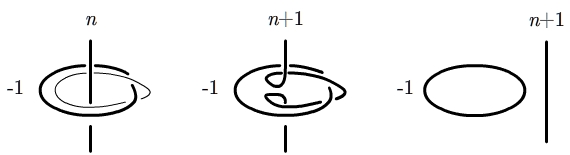
\includegraphics[scale=.6]{graphics/fenn-rourke-1}
\caption{Separating an unknotted component from a strand}
\label{fenn-rourke-1}
\end{figure}
\end{example}

\begin{example}
Suppose now there is an unknotted component of $L$ with framing $\pm 1$ that is linked once with \emph{two} strands from other components of $L$. All the steps are shown in \cref{fenn-rourke-2}. We can see that separating this unknotted component resulted in a full right twist in the two strands. If the two strands belong to two different link components, then each of their framings will increase by 1, and if they belong to the same component, the framing will increase by 2.

\begin{figure}[tb]
\centering
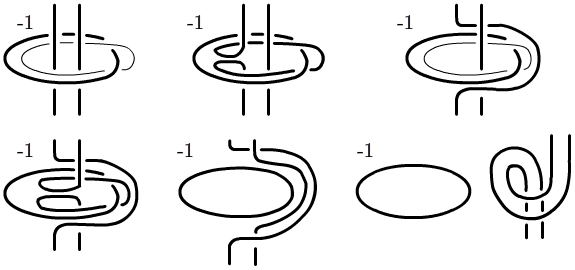
\includegraphics[scale=.6]{graphics/fenn-rourke-2}
\caption{Separating an unknotted component from two strands}
\label{fenn-rourke-2}
\end{figure}
\end{example}

\begin{example}
\label{the fenn-rourke move}
The general picture of the previous two examples is that if we can find an unknotted component of $L$ with framing $\pm 1$ that is linked once with $k$ strands, then we can separate the unknot from these strands by adding a full left/right twist in the strands, and changing their framings accordingly. This type of move (see \cref{fenn-rourke-3}) is called the \textbf{Fenn-Rourke move}. There is another name for this operation due to its relation to the 4-manifold theory of Kirby calculus. If we use the first Kirby move to introduce an unknotted, unlinked component with framing $\pm 1$, we say that we have performed a \textbf{blow-up} operation. Conversely, if we find an unknotted component with framing $\pm 1$ that links some strands once, then the operation of sliding the unknotted component off the strands and using $K_1$ to discard it is called the \textbf{blow-down} operation.

\begin{figure}[tb]
\centering
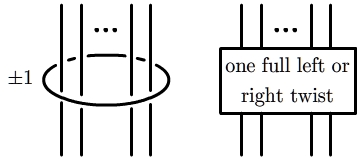
\includegraphics[scale=.6]{graphics/fenn-rourke-3}
\caption{Separating an unknotted component from many strands}
\label{fenn-rourke-3}
\end{figure}
\end{example}

\begin{example}
\label{removing unknotted 0-framed components}
Suppose our link $L$ can be written as $L = \cup_{i=0}^n L_i$ such that $L_0$ is the unknot with framing 0 and links with only $L_1$ once (the other $L_i$'s are free to link with $L_1$ in any way). We claim that we can use $K_2$ moves to change any crossing of some component $L_i$ ($i \geq 1$) passing \emph{under} $L_1$ to an over crossing. By changing all such crossings to over crossings we would have completely separated $L_0 \cup L_1$ from all of $\cup_{i=2}^n L_i$, and we would have completely unknotted $L_1$. 

Suppose a strand of $L_i$ crosses \emph{underneath} $L_1$. We can isotopy $L_0$ along $L_1$ so that it is close to this crossing (in a diagram we only need $R_1$ and $R_2$ moves). Sliding $L_i$ over $L_0$ and then applying $R_1$ and $R_2$ allows us to change this crossing to an over crossing (see \cref{removing-unknotted-0-frame}). If $i > 1$, then the framing of $L_i$ does change from this Kirby move since $L_0$ has framing 0 and $L_i$ is not not linked with $L_0$. However, if $i=1$, then the framing of $L_1$ is changed to $n_1 + 2\lk(L_0,L_1)$, where $n_1$ is the framing of $L_1$.

Once all the crossings have been changed so that $L_0 \cup L_1$ is separated from the rest of the link and $L_1$ is unknotted to become $L_1'$, we are left to deal with a Hopf link $L_0 \cup L_1'$ with one component framed by 0 and the other by some integer, say $p$. By sliding $L_1'$ over $L_0$ like we did above we see that the framing of $L_1'$ changes by $\pm 2$, so doing this repeatedly we can reduce this to the case when the Hopf link is framed by 0 and 1, or 0 and 0. Performing surgery on either of these links just gives $S^3$, so we can remove them entirely. In the end, we have separated $L_0 \cup L_1$ from the rest of $L$ and cancelled it.

\begin{figure}[tb]
\centering
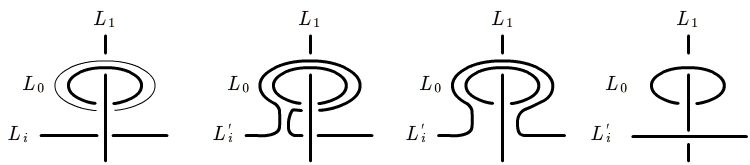
\includegraphics[scale=.6]{graphics/removing-unknotted-0-frame}
\caption{Changing under crossings to over via a 0-framed unknot}
\label{removing-unknotted-0-frame}
\end{figure}
\end{example}

\begin{example}
\label{unknotted 0-framed components and connected sums}
There is a simple way of expressing a surgery on the connected sum of two knots $k_1 \# k_2$ and the surgery on each knot separately. Suppose $k_1$ and $k_2$ have framings $p$ and $q$ respectively, and are linked once by a 0-framed unknot $k_0$. If we slide $k_1$ over $k_2$ to get $k_1'$, then we see that $k_0$ now only links $k_2$. So, applying the move in \cref{unknotted 0-framed components and connected sums} allows us to separate $k_0 \cup k_2$ from $k_1'$ and cancel it. The knot that is left, $k_1'$, is precisely $k_1 \# k_2$ with framing $p+q$. See \cref{connected-sum-surgery}. \todo{make this pic}
\end{example}

A graph embedded in the plane with vertices $v_i$ decorated by elements $p_i \in \mathbb Q \cup \lcb \infty \rcb$ induces a surgery diagram in the following way. Place an unknotted, unlinked circle $k_i$ at each vertex $v_i$ and frame it by $p_i$. If two vertices are connected by an edge, then link the corresponding circles once. If the graph is a tree, then there is a unique way to do this. These surgery tries provide a simply way to express surgery diagrams that are composed of unknotted components linked together in the simplest way.

We have seen that a surgery on any knot with framing $\pm 1$ results in an integral homology sphere. There is a particular homology sphere that is ubiquitous in low dimensional topology called the Poincar\'{e} sphere. We will define it to be the space obtained by surgery on the left-hand trefoil with framing $-1$. 

\begin{example}
We will show that the Poincar\'{e} sphere is homeomorphic to performing surgery on the $E_8$ Dynkin diagram where each vertex is framed by $-2$. We blow down this diagram three times by adding 3 unknotted components with framings $+1$ and sliding them over the 3 ends of the diagram. Then we blow up 8 times to remove all components with framing $-1$. At this point we have 3 components with framing 3, 2 and 5 linked to a component with framing 1. Blowing this up we get two components with framing 2 and 4 linked to a component with framing 1. Blowing up again gives a component of framing 3 linked with a component of framing 1, and a final blow of gives a single knot with framing 2. Performing a few $R_1'$ moves gives the trefoil with framing $-1$. \todo{make pic}
\end{example}




\subsection{The Rational Calculus}
\label{The Rational Calculus}


Now we will extend our moves on integral surgeries to rational surgeries. The first move we will consider is called a \textbf{Rolfsen twist}. Recall that the lens spaces $L(p,q)$ and $L(p,q+np)$ are homeomorphic for any integer $n$; that is, the surgeries on the unknot with rational coefficients $\frac{p}{q}$ and $\frac{p}{np + q}$ are homeomorphic. We will describe how to explicitly visualize this homeomorphic, which will then lead us to a new move on rational surgeries.

Let $H$ be the standardly embedded solid torus in $S^3$ and $T$ its boundary torus. We can construct $L(p,q)$ by a $p/q$ surgery on the unknot in $S^3$, which is equivalent to gluing two solid tori together via a map $f : T \rightarrow T$ that maps the meridian $\mu$ to the curve $q\mu+p\ell$, where $\ell$ is the longitude. If $\tau : T \rightarrow T$ is a right Dehn twist around $\mu$, then each time the curve $q\mu+p\ell$ intersects $\mu$ (which is $p$ times) the curve $\tau(q\mu+p\ell)$ picks up another intersection with $\ell$, hence $\tau(q\mu+p\ell) = (q+p)\mu + p\ell$. Since $\tau$ extends to a homeomorphism of the solid torus $H$ that $T$ bounds we have that it also extends to a homeomorphism of $H \cup_f H$ and $H \cup_{\tau \circ f} H$ by our gluing lemma (\cref{technical gluing lemma}). This shows explicitly that $L(p,q)$ is homeomorphic to $L(p,p+q)$. We can generalize this construction by letting $\tau$ be an $n$-fold Dehn twist around $\mu$ (where it is a right twist if $n>0$ and a left twist if $n<0$), in which case we get an explicit homeomorphism of $L(p,np+q)$ with $L(p,q)$. If $r=p/q$, then we can also rephrase this as the $r$ surgery on the unknot is homeomorphic to the $\frac{1}{n + \frac{1}{r}}$ surgery on the unknot for any $n$.

We can now describe the Rolfsen twist. Suppose we have a rationally framed link in $S^3$ such that one component $k$ is framed with an integer $n$ and is linked once with an unknotted component $U$ which has any rational framing $r=p/q$. We claim that surgery on this link is equivalent to surgery on the link formed by changing $k$'s framing to $n \pm 1$ and $U$'s framing to $\frac{p}{\pm p + q} = \frac{1}{\pm 1 + \frac{1}{r}}$. We will show this by mimicking the above arguments to describe an explicit homeomorphism between the spaces. 

First we remove a tubular neighborhood $\nu U$ of $U$ from $S^3$ to obtain the space $X$, and let $f : \partial \nu U \rightarrow \partial X$ be the gluing homeomorphism for the surgery on $U$; that is, $f$ maps the meridian of  $\partial \nu U$ to $q$ times around the meridian and $p$ times around the longitude of $\partial X$. Let $\tau$ be the homeomorphism of $X$ that cuts the space open along a disc $D \subset X$ such that $\partial D$ is the longitude on $\partial \nu U$, performs a full right twist, then glues everything back, and is the identity outside a small ball containing $D$. Now glue $U$ back into $X$ via the map $\tau \circ f$. Then clearly this surgery is equivalent to the original surgery, except now $U$ is framed by $\frac{p}{p+q}$ and $k$ is framed by $n+1$.

\begin{figure}[tb]
\centering
\ \ \ \ \ \ \ \ \ \ \ \ \ \ \ \ 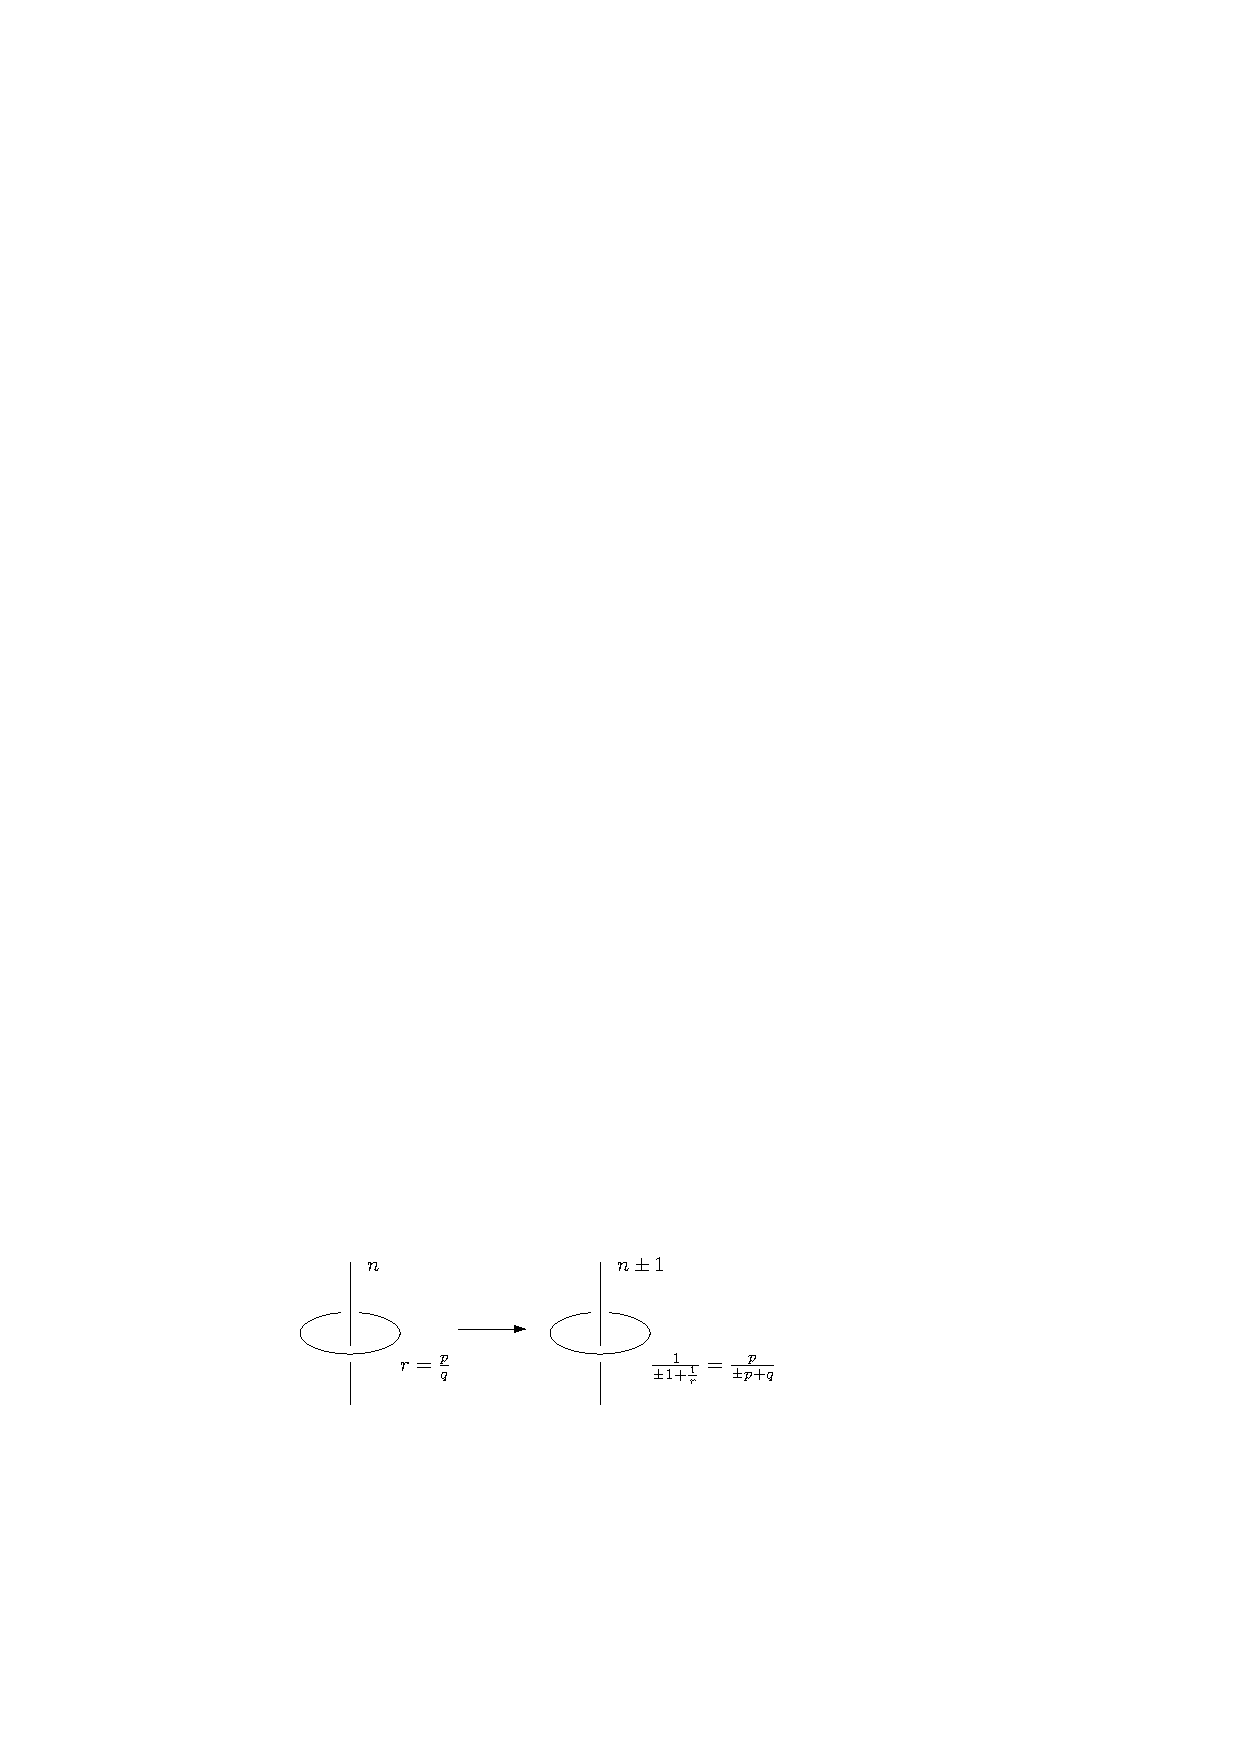
\includegraphics[scale=1]{graphics/rolfsen-twist}
\caption{The Rolfsen Twist}
\label{rolfsen-twist}
\end{figure}

There is another rational calculus move that will be helpful called the \textbf{slam dunk} move. It can be derived from the Rolfsen twist, but we can also see it directly. Suppose we are doing surgery on a link $k_1 \cup k_2$, where $k_1$ has framing $n \in \mathbb Z$ and $k_2$ has framing $r \in \mathbb Q \cup \lcb \infty \rcb$. Further, suppose $k_2$ is a meridian of $k_1$. Then we claim that performing surgery on $k_1 \cup k_2$ is equivalent to performing surgery on only $k_1$, but now with framing $n - \frac{1}{r}$ (see \cref{slam-dunk}). To see this let us first perform surgery on $k_1$ by gluing a solid torus $T$ into the complement of $k_1$ to obtain a manifold $M$, and now $k_2$ is a knot in $M$. Now, pull $k_2$ in $T$; since we performed an integral surgery on $k_1$ we have that $k_2$ (having been pulled into $T$) intersects a compressing disc $\lcb * \rcb \times D^2$  of $T$ in exactly one point, and so we can isotope it to the curve $S^1 \times \lcb 0 \rcb$ in $T$. Now $T$ is a tubular neighborhood for $k_2$, and so to perform surgery on it we cut out and reglue $T$, hence the result of performing surgery on $k_1 \cup k_2$ is the same as performing surgery only on $k_1$. Now we have to figure out the framing of $k_2$. Note that if $n$ where 0, then we glue $T$ in by a map sending $\mu \mapsto \ell$ and $\ell \mapsto -\mu$. If we follow this we the gluing determined by the framing $r=p/q$ we see that the net result is $\mu \mapsto -q\mu+p\ell$, which is the framing $-\frac{1}{r}$. More generally the framing changes to $n - \frac{1}{r}$.

\begin{figure}[tb]
\centering
\ \ \ \ \ \ 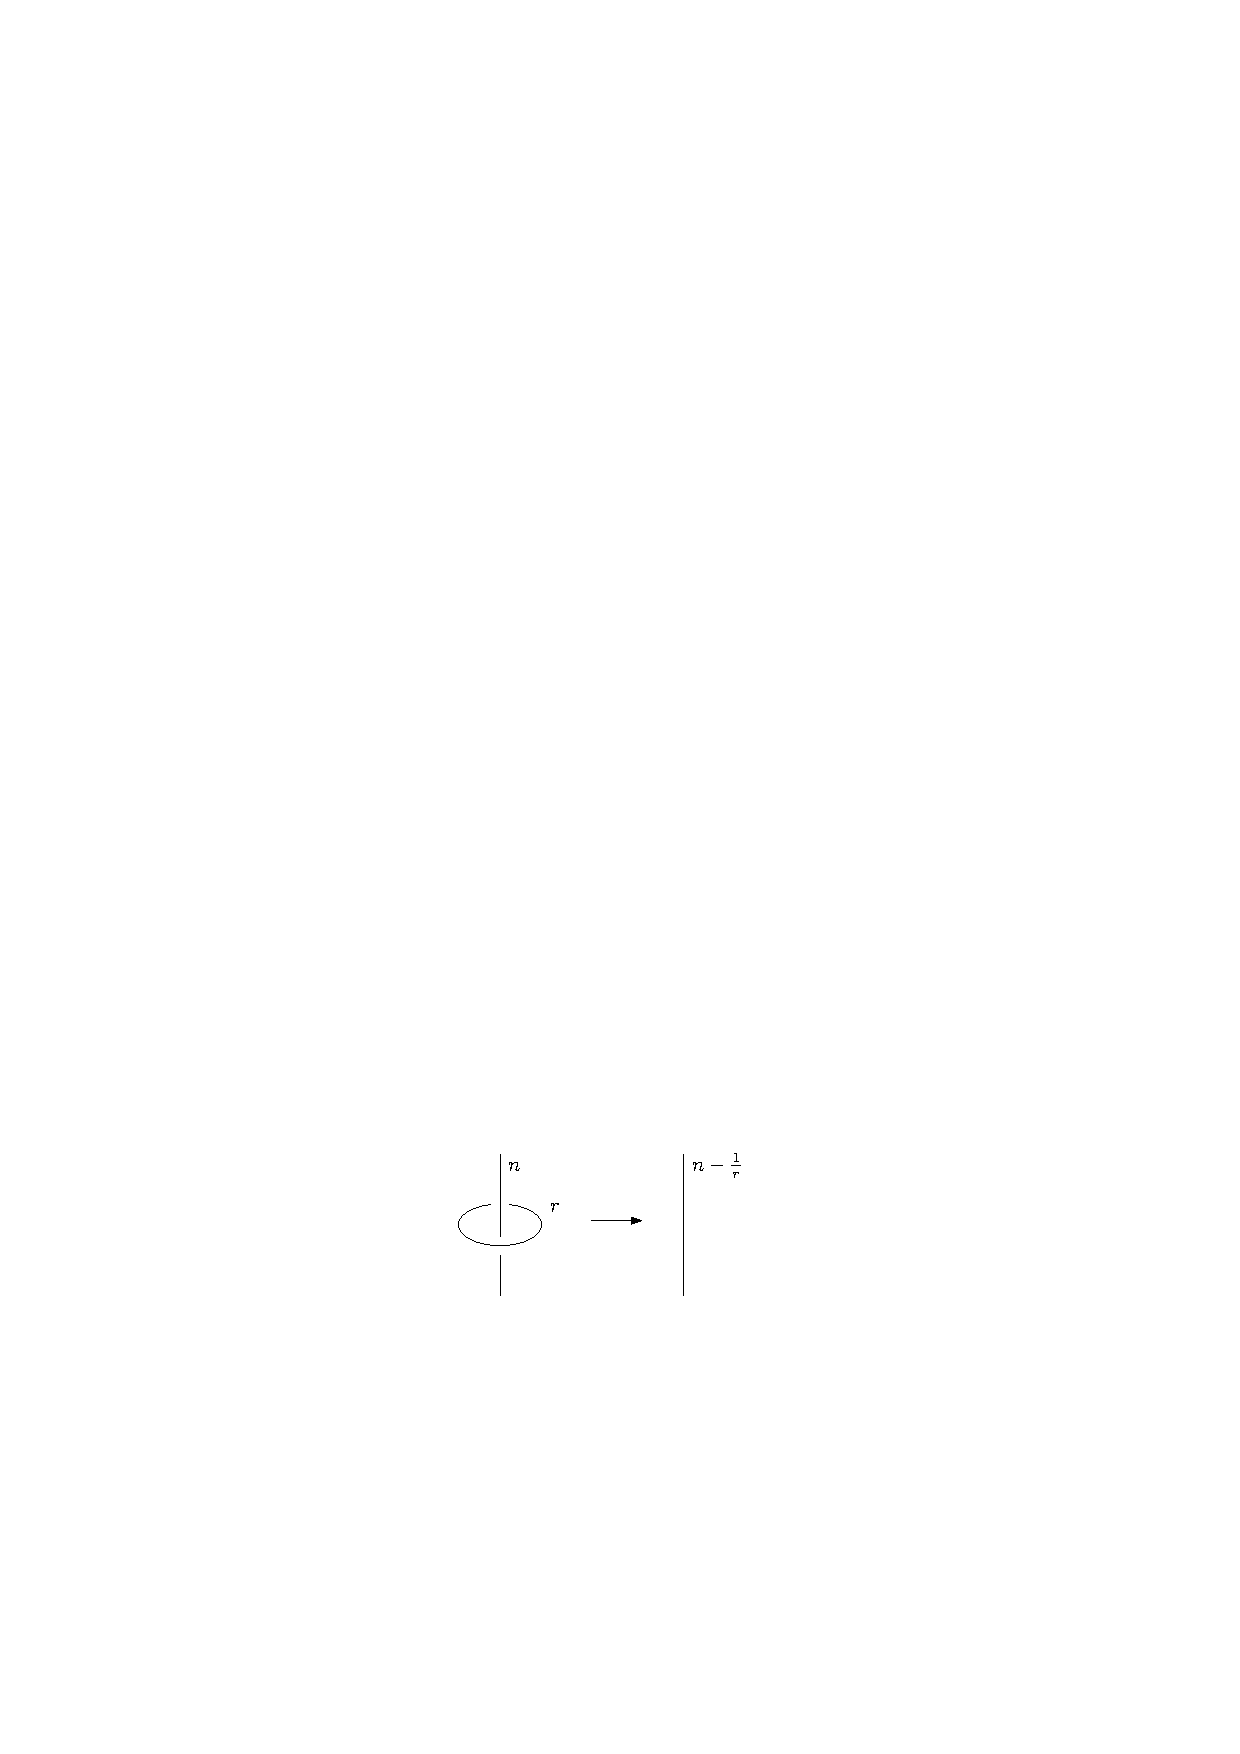
\includegraphics[scale=1]{graphics/slam-dunk}
\caption{The Slam Dunk}
\label{slam-dunk}
\end{figure}


It turns out that the Rolfsen twists are nearly enough to get between any rational surgery diagrams for the same 3-manifold.
\begin{thm}
If two 3-manifolds presented as a rational surgery diagram are orientation preservingly diffeomorphic, then one diagram can be brought into the other via a finite sequence of Rolfsen twists and adding/removing a knot component with framing $\infty$.
\end{thm}

Let us look at many examples using these rational calculus moves.

\begin{example}
Let us find an integral surgery diagram for the lens spaces $L(p,q)$, which we know is the $p/q$ surgery on the unknot. First write $p/q$ in its finite continued fraction expansion
\begin{equation}
\label{continued fraction expansion}
\frac{p}{q} = a_1 - \cfrac{1}{a_2 - \cfrac{1}{a_3 - \cfrac{1}{a_4 - \cfrac{1}{\ddots\, - \cfrac{1}{a_n}}}}} 
\end{equation}
where $a_1,\ldots,a_n$ are integers. We will use the notation $[a_1,\ldots,a_n]$ to denote a continued fraction expansion. We claim that surgery on the diagram in \cref{lens-space-integral-surgery} produces the lens space $L(p,q)$. To see this perform a slam dunk on the last component to obtain a link with $(n-1)$ components. The framings of these components are the same as the original link, except the last component now has framing $a_{n-1} - \frac{1}{a_n}$. Performing a slam dunk on this component gives a link with $(n-2)$ components, and the last framing is now
\[ a_{n-2} - \cfrac{1}{a_{n-1} - \cfrac{1}{a_n}} \]
Continuing this until we have only one component in the link leaves us with an unknot with framing given precisely by \eqref{continued fraction expansion}.

\begin{figure}[tb]
\centering
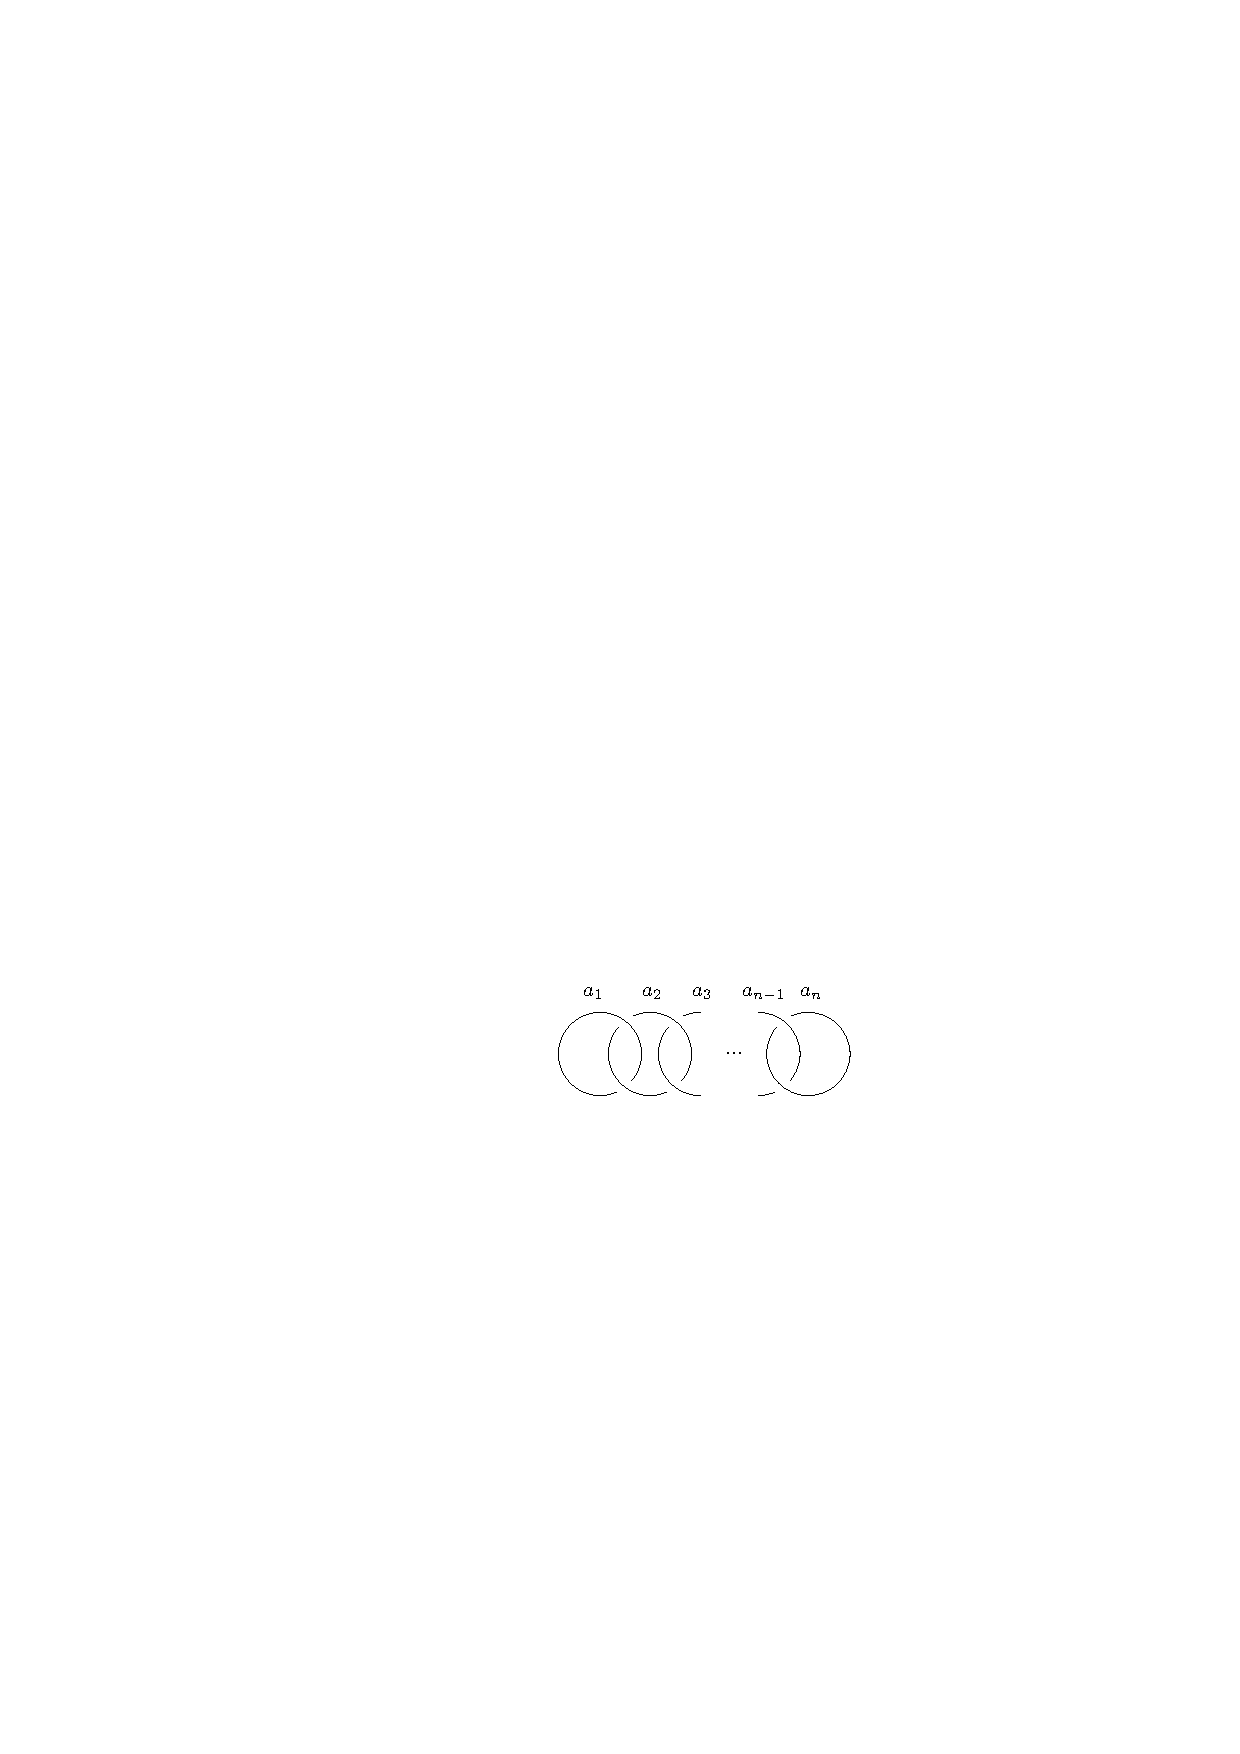
\includegraphics[scale=1]{graphics/lens-space-integral-surgery}
\caption{Surgery Diagram for $L(p,q)$}
\label{lens-space-integral-surgery}
\end{figure}

\end{example}


\begin{example}
We can use the idea developed in the previous example to turn any rational surgery diagram into an integral surgery diagram by adding unknot components. In particular, suppose there is a knot $k$ in our diagram with framing $r \in \mathbb Q$, and let $r = [a_1,\ldots,a_n]$ be its continued fraction expansion. Then we can change the framing of $k$ to $a_1$, and attach a link of $(n-1)$ unknotted components with framings $a_2,\ldots,a_n$, as shown in \cref{rational-to-integral-surgery}.

\begin{figure}[tb]
\centering
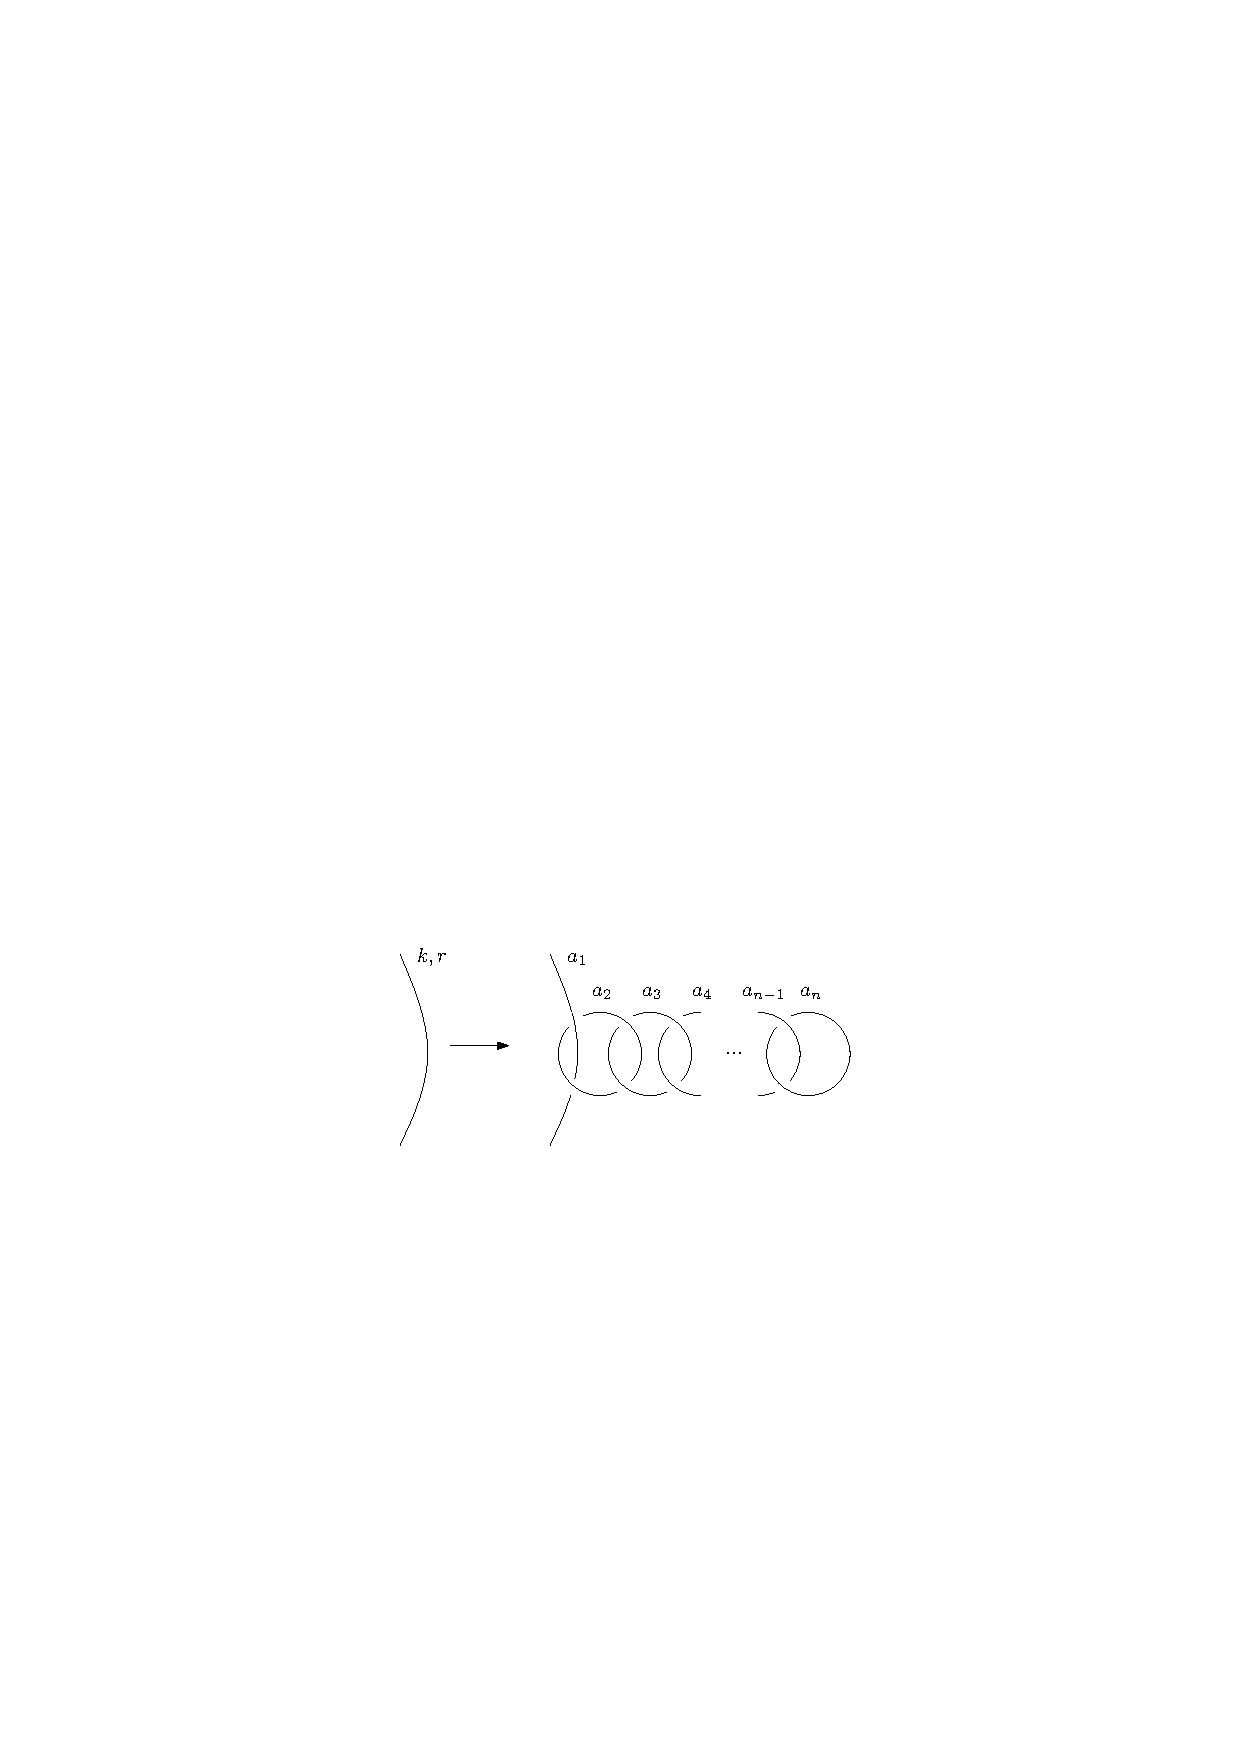
\includegraphics[scale=1]{graphics/rational-to-integral-surgery}
\caption{Changing a rational surgery to an integral surgery}
\label{rational-to-integral-surgery}
\end{figure}
\end{example}



\begin{example}
Let us show that $L(7,3)$ is homeomorphic to $L(7,4)$ via an orientation \emph{reversing} homeomorphism. We have the continued fraction expansion $\frac{7}{4} = 2 + \frac{1}{3}$, hence $L(7,3)$ is a surgery on a Hopf link with framings $2$ and $-3$. On the other hand we have $\frac{7}{4} = 1 + \frac{1}{1 + \frac{1}{3}}$, hence $L(7,4)$ is a surgery on a 3 component Hopf link with framings $1$, $-1$ and $3$. If we blow down the middle link we get a Hopf link with framings $-2$ and $3$. This describes a manifold diffeomorphic to $L(7,3)$, but with the opposite orientation.
\end{example}









\newpage
\section{4-Manifold Theory}
\label{4-Manifold Theory}




\subsection{Intersection Forms on 4-Manifolds}
\label{Intersection Forms on 4-Manifolds}


Let $M$ be a closed, oriented, connected and simply connected 4-manifold, and let $[M]$ denote its fundamental class. Since $M$ is simply connected we have $H_1(M) = 0$, hence $H^3(M) = 0$ by Poincar\'{e} duality. Further, the split exact sequence of the universal coefficient theorem says that
\[ H^2(M) = \Ext(H_1(M),\mathbb Z) \oplus \Hom(H_2(M),\mathbb Z) = \Hom(H_2(M),\mathbb Z) \]
Since $\Hom(A,B)$ is torsion free if $B$ is free, we have that $H^2(M)$ is torsion free, and hence $H_2(M)$ is torsion free by Poincar\'{e} duality. Define a bilinear form $Q_M : H^2(M) \otimes H^2(M) \rightarrow \mathbb Z$ by
\[ Q_M(\alpha,\beta) = (\alpha \smallsmile \beta, [M]) \]
This symmetric bilinear form is called the \textbf{intersection form} of $M$. This form is non-degenerate, which means that its matrix in \emph{any} basis is non-singular, i.e. determinant $= \pm 1$. 

There is a more geometric way of defining this bilinear form in terms of counting intersections of embedded surfaces. If $M$ is a closed, smooth, oriented $n$-manifold, we say that a homology class $a \in H_k(M)$ is \emph{represented} by an oriented, smoothly embedded $k$-submanifold $i : N \rightarrow M$ if $i_*[N] = a$. Then we have the following
\begin{lem}
\label{2nd homology classes represented by surfaces}
Let $M$ be a closed, oriented, smooth 4-manifold. Any homology class $a \in H_2(M)$ can be represented by a smoothly embedded surface in $M$.
\end{lem}
\begin{proof}
We will prove this for the case when $M$ is simply connected, which is the case we need the most for our later discussions. Since $M$ is simply connected, the Hurewicz homomorphism $h : \pi_2(M) \rightarrow H_2(M)$ is an isomorphism. Recall that this map is defined by $h([f]) = f_*[S^2]$, so every homology class $\alpha \in H_2(M)$ has a corresponding classifying map $f : S^2 \rightarrow M$ such that $f_*[S^2] = \alpha$. Since $\dim M = 4$ we have that $f$ can be slightly homotoped so that $f$ is an immersion with finitely many isolated double points. Locally, a double point looks like two planes in $\mathbb R^4$ intersecting at a point $P$. We can cut a small disc out of each plane around $P$ and connect the planes with a cylinder that misses $P$. Performing this operation on each double point of $f(S^2)$ we get a smoothly embedded surface in $M$ representing $\alpha$.
\end{proof}


So, for a 4-manifold $M$ and two homology classes $a,b \in H_2(M)$, let $F_a,F_b \subset M$ be smoothly embedded, oriented surfaces representing $a$ and $b$ respectively. We can slightly deform the embeddings, if necessary, so that $F_a$ and $F_b$ intersect transversally in a finite collection of points. Assign a sign of $\pm 1$ to each intersection point $p$ depending on whether or not the induced orientation on $T_p F_a \oplus T_p F_b$ from $F_a$ and $F_b$ agrees with $T_p M$. We call the sum of these numbers the \emph{intersection product} of $a$ and $b$, and denote it by $a \cdot b$. Then
\begin{prop}
$Q_M(\alpha,\beta) = PD(\alpha) \cdot PD(\beta)$
\end{prop}

If we fix a basis $e_1,\ldots,e_k$ of $H_2(M)$, then we call the matrix $[Q_M] = \lcb e_i \cdot e_j \rcb_{ij}$ the matrix form of $Q_M$. It is clearly symmetric.

\begin{example}
Let $M = S^2 \times S^2$, then $H_2(M)$ is generated by $a = S^2 \times \lcb y_0 \rcb$ and $b = \lcb x_0 \rcb \times S^2$ for some base point $(x_0,y_0) \in M$. We can slightly deform $a$ to be completely disjoint from the original $a$, hence $a \cdot a = 0$, and similarly $b \cdot b = 0$. We cannot deform $a$ so that it is disjoint from $b$, but $a$ and $b$ clearly intersect transversally at one point, and by choosing orientations appropriately we have $a \cdot b = 1$. Therefore the matrix form of $Q_M$ with respect to the basis $a,b$ is
\[ [Q_M] = \begin{pmatrix} 0 & 1 \\ 1 & 0 \end{pmatrix} \]
\end{example}

\begin{example}
We will see soon that the intersection form on $\mathbb CP^2$ is $(1)$ and on $\overline{\mathbb CP}^2$ is $(-1)$. More generally, the intersection form on the $D^2$-bundle over $S^2$ with Euler number $n$ is just $(n)$. 
\end{example}

\begin{example}
An easy application of the Mayer-Vietoris sequence shows that $H_2(M \# N) \cong H_2(M) \oplus H_2(N)$, and so $Q_{M \# N} = Q_M \oplus Q_N$.
\end{example}


If $M$ is a compact, oriented, connected and simply connected 4-manifold with boundary, then $H^2(M)$ and $H^2(M,\partial M)$ are still torsion free, and so Poincar\'{e}-Lefschetz duality gives us a non-degenerate pairing $Q_M : H^2(M) \otimes H^2(M,\partial M) \rightarrow \mathbb Z$ defined by $Q_M(\alpha,\beta) = (\alpha \smallsmile \beta,[M,\partial M])$. If $\partial M$ is an integral homology sphere, then $H^2(M,\partial M) = H^2(M)$, and so $Q_M$ is a symmetric, non-degenerate pairing of $H^2(M)$ with itself. In terms of intersections of surfaces, we can still define the intersection product $\cdot : H_2(M) \otimes H_2(M) \rightarrow \mathbb Z$ in the usual way, and if $M$ is an integral homology sphere we still have $Q_M(\alpha,\beta) = PD(\alpha) \cdot PD(\beta)$. There is a converse to the non-degeneracy of $Q_M$.
\begin{prop}
The intersection form $Q_M$ on a compact, oriented, connected and simply connected 4-manifold $M$ with boundary is non-degenerate if and only if $\partial M$ is an integral homology sphere.
\end{prop}
\begin{proof}
If $\partial M$ is a disjoint union of integral homology spheres, then we have already seen that $Q_M$ is non-degenerate by Poincar\'{e}-Lefschetz duality.

Suppose $Q_M$ is non-degenerate. Since $M$ is simply connected we have $H^1(M)=0$ by the universal coefficient theorem, hence $H_3(M,\partial M)=0$ by Poincar\'{e}-Lefschetz duality. A part of the long exact sequence of the pair $(M,\partial M)$ looks like
\[ 0 \longrightarrow H_2(\partial M) \stackrel{i_*}{\longrightarrow} H_2(M) \stackrel{j_*}{\longrightarrow} H_2(M,\partial M) \longrightarrow H_1(\partial M) \longrightarrow 0 \]
So we have $i_*$ is injective, hence $\image i_* = 0$ if and only if $H_2(\partial M)=0$. If $\image i_*$ were not trivial, then for any $a \in \image i_*$ and $b \in H_2(M)$ we have $a \cdot b = 0$ since we can move any surface representing $b$ so that it does not intersect the boundary at all. But, $Q_M$ is assume to be non-degenerate, so we do not allow this to happen, hence $\image i_* = 0$, and so $H_2(\partial M)=0$. Finally, this implies $H_1(\partial M)=0$, therefore $\partial M$ is an integral homology sphere.
\end{proof}

Intersection forms are very important in 4-dimensional topology. In fact, they nearly classify all simply connected 4-manifolds by a theorem of Freedman. So, it will be useful to recall some basic facts of non-degenerate, symmetric, bilinear forms $Q : \mathbb Z^n \times \mathbb Z^n \rightarrow \mathbb Z$. We say that two such forms $Q_1,Q_2$ are isomorphic if there is an isomorphism $\varphi : \mathbb Z^n \rightarrow \mathbb Z^n$ such that $Q_1(x,y) = Q_2(\varphi(x),\varphi(y))$. The rank of $Q$ is defined to be $n$. If we think of $Q$ as a bilinear form over $\mathbb R$, then we can diagonalize over the reals and there will be $b_+$ positive values and $b_-$ negative values on the diagonal. These numbers are invariants of the isomorphism type of $Q$, as is the signature $\sign Q = b_+-b_-$. We call $Q$ a \textbf{definite} form if $b_-=0$ or $b_+=0$, and call $Q$ an \textbf{indefinite} form otherwise. We say that $Q$ is \textbf{even} if $Q(x,x)=0 \modulo 2$ for all $x$, and otherwise we say $Q$ is \textbf{odd}.

There is a nice relationship between surgeries on links and intersection forms on cobordisms of surgeries. First we will consider a fourth way of defining the linking number of two disjoint, oriented knots (see the other three definitions in \cref{Basic Definitions}). For disjoint, oriented knots $k_i$ and $k_j$ in $S^3$, let $F_i$ and $F_j$ be Seifert surfaces with their induced orientations. We can push the interiors of these surfaces into the 4-ball $D^4$ that bounds $S^3$ so that $F_i \cap S^3 = k_i$ and $F_j \cap S^3 = k_j$. Then, perturbing $F_i$ and $F_j$ slightly so that they intersect transversely if necessary, one can compute that $\lk(k_i,k_j) = F_i \cdot F_j$. 

Let $X$ be a 4-dimensional 2-handlebody; that is, a 4-manifold that can be decomposed as 0-handle $\cup$ 2-handles $\cup$ 4-handle. This is equivalent to specifying a link $L = k_1 \cup \cdots \cup k_n$ in $\partial D^4$ with $k_i$ framed by an integer $p_i$. For each component $k_i$, let $F_i$ denote a surface of $k_i$ embedded in $\partial D^4 = S^3$, then we can push this surface a little bit into $D^4$ to obtain a surface $\hat F_i$ such that $\hat F_i \cap S^3 = \partial \hat F_i = k_i$. Let $G_i$ be the core disc of $h_i$, then by gluing $\hat F_i$ and $G_i$ together along $k_i$ we obtain a closed, oriented, smoothly embedded surface $\alpha_i$ in $X$. Put any orientation on $k_i$, then we get induced orientations on $\hat F_i$ and $G_i$, hence $\alpha_i$ also gets an induced orientation.

\begin{prop}
The surfaces $\alpha_1,\ldots,\alpha_n$ form a basis for $H_2(X)$.
\end{prop}
\begin{proof}
First consider the space obtained from attaching one 2-handle $Y = D^4 \cup_{\varphi} (D^2 \times D^2)$. Let $N$ be a small open neighborhood of $\varphi(\partial D^2 \times D^2)$, and let $U = D^4 \cup N$ and $V = (D^2 \times D^2) \cup N$. Then $U$ is homotopy equivalent to $D^4$, $V$ is homotopy equivalent to $D^2 \times D^2$, and $U \cap V$ is homotopy equivalent to $S^1 \times D^2$. The Mayer-Vietoris sequence gives the following exact sequence.
\[ H_2(U) \oplus H_2(V) \longrightarrow H_2(Y) \stackrel{\Delta}{\longrightarrow} H_1(U \cap V) \longrightarrow H_1(U \oplus V) \]
which implies that the connecting homomorphism $\Delta : H_2(Y) \rightarrow H_1(U \cap V)$ is an isomorphism, where clearly $H_1(U \cap V) \cong \mathbb Z$. To understand the generator of $H_2(Y)$ let us recall how the connecting homomorphism is defined. A cycle $c \in Z_2(Y)$ can be expressed as $c = u+v$ with $u \in C_2(U)$ and $v \in C_2(V)$. This implies $\partial u = -\partial v$, hence $\partial u \in Z_1(U \cap V)$, and so we define $\Delta[c] = [\partial u]$. 

The attaching sphere knot $k$ of the 2-handle is the generator of $H_1(U \cap V)$, so we need to determine what element $\alpha$ of $H_2(Y)$ gets mapped to $k$. By our description of $\Delta$ we see that $\alpha$ can be represented by a 2-chain in $U$ and a 2-chain in $V$ whose boundaries are $k$. Therefore we can take these chains to be the Seifert surface of $k$ pushed into $D^4$ and the core disc of the 2-handle $D^2 \times D^2$, and so $\alpha$ is can be represented by gluing these surfaces together.

Repeating this argument for each 2-handle in $X$ we get a set of $n$ generators of $H_2(X)$, which we know to be of rank $n$ from its handlebody homology, therefore these generators form a basis.
\end{proof}

We call the basis $\alpha_,\ldots,\alpha_n$ the canonical basis of $H_2(X)$. Let us compute the matrix of the intersection form with respect to this canonical basis. First we compute the self intersection number $\alpha_i \cdot \alpha_i$. Translate the core disc $G_i$ to a parallel disc $G_i'$ in the boundary $D^2 \times \partial D^2$. This new disc will intersect the boundary of $D^4$ at a longitude of $k_i$, call it $k_i'$, with linking number $\lk(k_i,k_i')=p_i$. Isotope the Seifert surface $F_i$ to a new surface $F_i'$ such that $\partial F_i' = k_i'$, and then push this surface into $D^4$ to obtain $\hat F_i'$ such that $\hat F_i' \cap S^3 = \partial \hat F_i' = k_i'$ and so that $\hat F_i$ and $\hat F_i'$ intersect transversally. By gluing $\hat F_i'$ to $G_i'$ we obtain a closed surface $\alpha_i'$ that represents the same homology class as $\alpha$, and clearly
\[ \alpha_i \cdot \alpha_i' = (\hat F_i \cup G_i) \cdot (\hat F_i' \cup G_i') = F_i \cdot F_i' = \lk(k_i,k_i') = p_i \]
Repeating this argument for two different components $k_i$ and $k_j$, shows that $\alpha_i \cdot \alpha_j = \lk(k_i,k_j)$. So, we have proved the following.
\begin{prop}
\label{intersection form = linking matrix}
The intersection form of a 2-handlebody in the canonical basis is equal to the linking matrix of the associated link.
\end{prop}

Let $M = \partial X$, i.e. $M$ is the result of performing the surgery on the link $L$ in $S^3$. We saw in \cref{first homology of integral surgery} that $H_1(M)$ could be computed as $\mathbb Z^n / \image [L]$, where $[L]$ is the linking matrix of $L$. As a corollary we now have
\begin{cor}
Let $X$ be a 2-handlebody with intersection form $Q_X$. Then $H_1(\partial X)$ is finite if and only $\det Q_X \neq 0$, in which case $|H_1(\partial X)| = |\det Q_X|$. 
\end{cor}







\subsection{Kirby Calculus Reinterpreted}
\label{Kirby Calculus Reinterpreted}


Kirby calculus is essentially a 4-dimensional technique, and so we take another look at the Kirby moves. To bring Kirby calculus into the 4-dimensional world we show that surgeries on manifolds induce cobordisms. Recall that two compact, oriented, smooth $n$-manifolds $M_1$ and $M_2$ are said to be \textbf{cobordant} if there is a compact, oriented, smooth $(n+1)$-manifold $W$ such that $\partial W = -M_1 \sqcup M_2$, where $-M_1$ is $M_1$ with the opposite orientation. A manifold $M$ is said to be \textbf{cobordant to zero} if it is cobordant to the empty manifold, i.e. $\partial W = M$.

\begin{prop}
\label{surgery attaching 2-handle proposition}
The manifold resulting from any surgery on any knot in $S^3$ is cobordant to zero.
\end{prop}
\begin{proof}
Let $k$ be a knot in $S^3$ with tubular neighborhood $N(k)$, and let $\varphi : \partial(S^1 \times D^2) \rightarrow \partial(M \backslash N(k))$ be the attaching map that determines the surgery on $k$. Let $c$ be the image of any meridian $\lcb * \rcb \times \partial D^2$ under $\varphi$ so that $c$ is a curve in $\partial N(k)$. There is a diffeomorphism $\phi : \partial D^2 \times D^2 \rightarrow N(k)$ such that $\phi(\partial D^2 \times \lcb 0 \rcb) = k$ and $\phi(\partial D^2 \times \lcb * \rcb) = c$, where $*$ is some point on the boundary of the 2-disc. Let $W$ be the manifold resulting from attaching the 2-handle $D^2 \times D^2$ to the the 4-ball $D^4$ via $\phi : \partial D^2 \times D^2 \rightarrow N(k) \subset \partial D^4$.

The boundary of the 4-ball has changed by attaching this 2-handle. The part of the boundary of $D^4$ outside of $N(k)$ (which is the knot complement) have remained boundary points, and all the points in $N(k)$ have now become interior points of $M$. The ``free'' part $D^2 \times \partial D^2$ of the boundary of the 2-handle have now become boundary points of $M$ (see \cref{surgery-cobordism-ball}). This means we have removed a solid torus from $M$ and glued in another solid torus. In fact, the solid torus was glued in by a diffeomorphism that maps the meridian $\partial D^2 \times \lcb * \rcb$ to the curve $c$, hence this is just performing the surgery on $k$ determined by $\varphi$. Therefore we have constructed a cobordism from the surgered manifold to the empty manifold, and so it is cobordant to zero. 

\begin{figure}[tb]
\centering
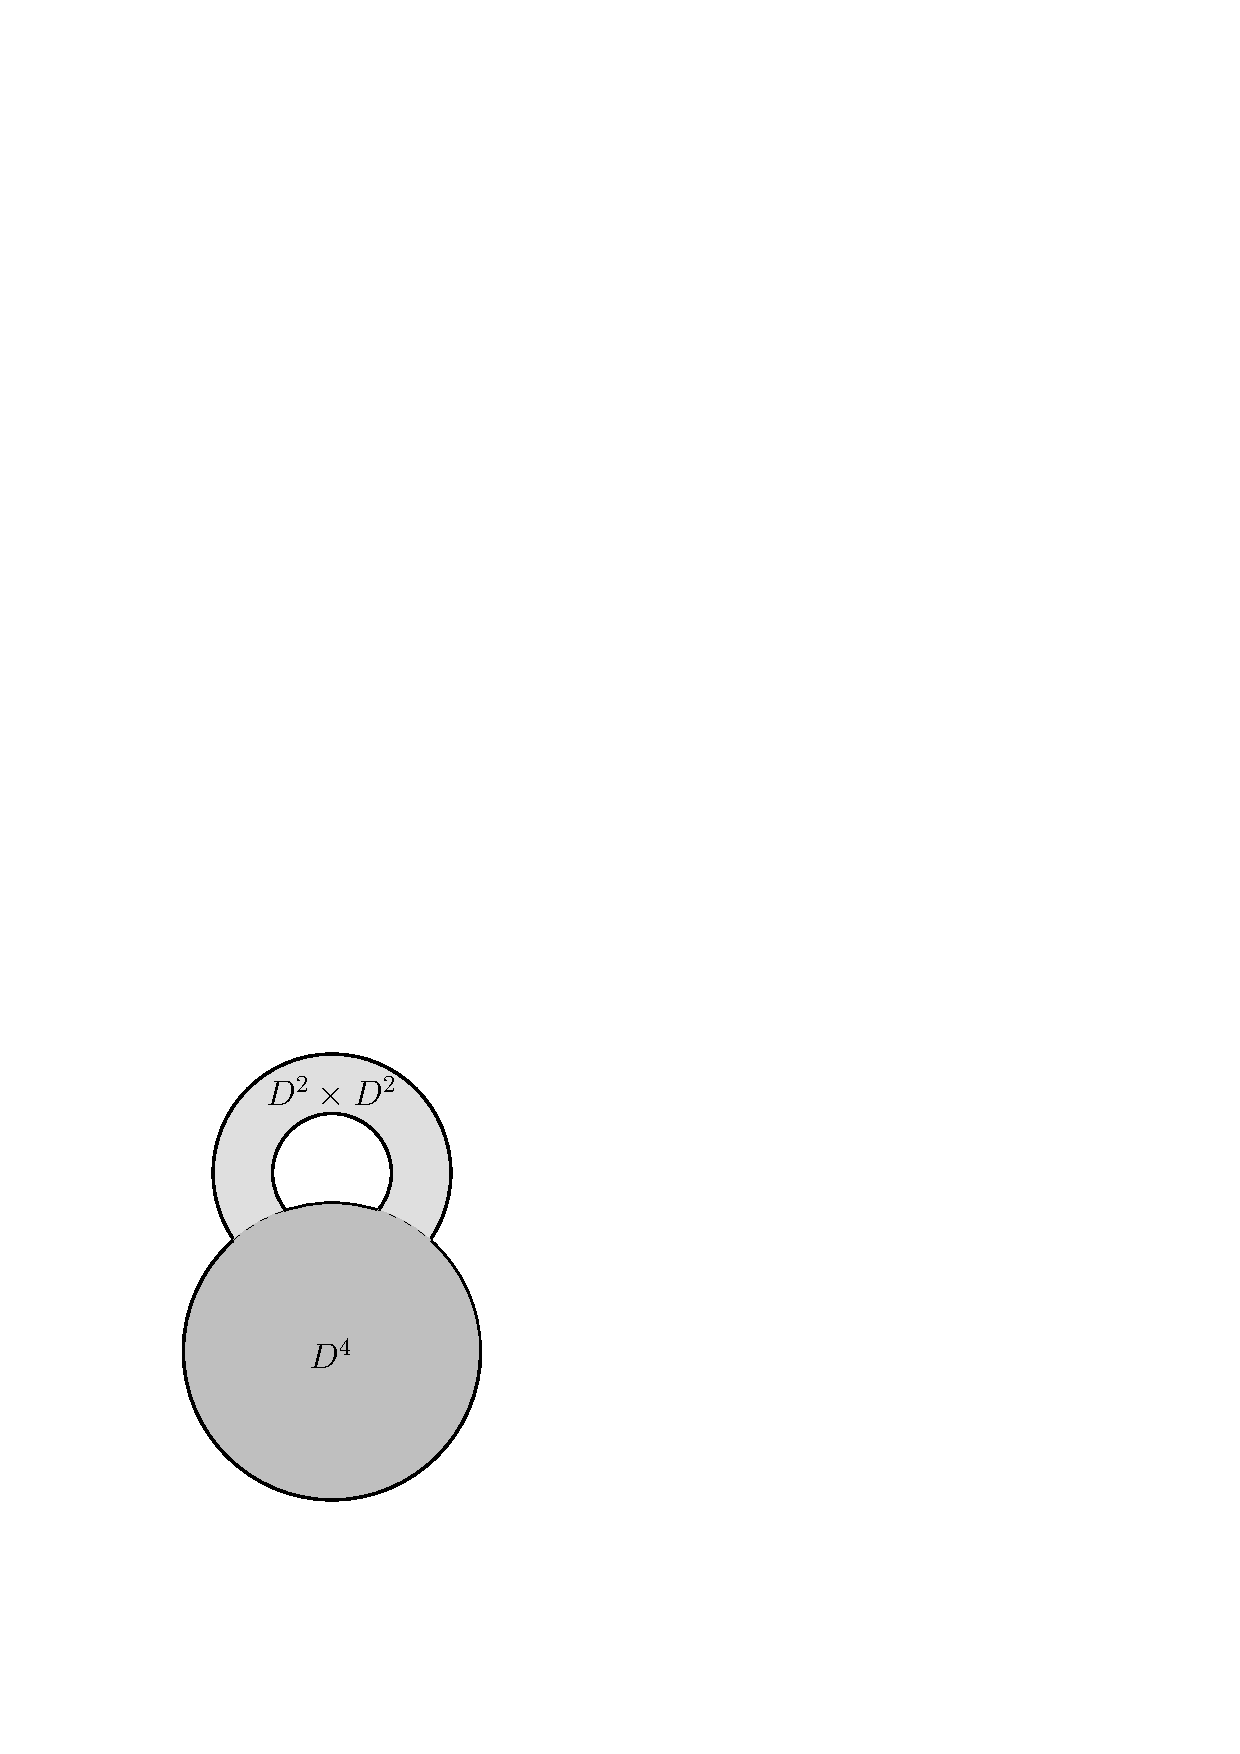
\includegraphics[scale=.6]{graphics/surgery-cobordism-ball}
\caption{Surgery Cobordism}
\label{surgery-cobordism-ball}
\end{figure}
\end{proof}


\begin{cor}
Every closed, oriented 3-manifold is cobordant to zero.
\end{cor}
\begin{proof}
By \cref{surgery attaching 2-handle proposition} we have that every surgery on $S^3$ is cobordant to zero. But, by \cref{Lickorish-Wallace theorem} every closed, oriented 3-manifold is a surgery on $S^3$, hence every such manifold is cobordant to zero.
\end{proof}

\begin{example}
\label{E_n spaces}
We saw earlier that $D^2$-bundles over $S^2$ are canonically parameterized by $\mathbb Z$ by attaching a 4-dimensional 2-handle along an unknotted circle in $\partial D^4$. Let $E_n$ denote this 4-manifold with boundary, and since $\partial E_n$ is the result of performing a surgery on the unknot with framing $n$, we see that $\partial E_n = L(n,1)$. In particular $E_0$ is the trivial bundle $S^2 \times D^2$. We also saw that $\mathbb CP^2$ is a union of a 0, 2 and 4-handle, and the 2-handle is attached to the 0-handle along an unknotted circle. So, which of the 4-manifolds $E_n$ corresponds to $\mathbb CP^2 \backslash D^4$, i.e. $\mathbb CP^2$ without its 4-handle? In $\mathbb CP^2$ the 2-handle $D^2 \times D^2$ is attached to $D^4 = D^2 \times D^2$ via the map $\varphi : \partial D^2 \times D^2 \rightarrow \partial (D^2 \times D^2)$ defined by $\varphi(z,w) = (\overline z, \overline zw)$. By fixing a $z$ and restricting $|w|=1$ we see that a longitude of $S^1 \times D^2$ is wrapped once around the meridian and once around the longitude of $S^1 \times D^2$. So, when we attach this handle the boundary changes by performing a surgery on the unknot with framing $+1$, hence $\mathbb CP^2 \backslash D^4$ is diffeomorphic to $E_1$. We also have $E_{-1}$ is diffeomorphic to $\overline{\mathbb CP}^2 \backslash D^4$. 
\end{example}

A slight generalization of the construction in \cref{surgery attaching 2-handle proposition} gives an explicit cobordism between any manifold and any surgery on that manifold.

\begin{cor}
\label{surgery cobordism proposition}
Any integral surgery on any 3-manifold $M$ is cobordant to $M$.
\end{cor}
\begin{proof}
Mimic the construction in \cref{surgery attaching 2-handle proposition} by attaching a 2-handle to the component $M \times \lcb 1 \rcb$ of the 4-manifold $M \times I$. After the handle is attached one component will be $M$ and the other component will be the result of the sugery (see \cref{surgery cobordism figure}).

\begin{figure}[tb]
\centering
\ \ \ \ \ \ \ \ \ \ \ 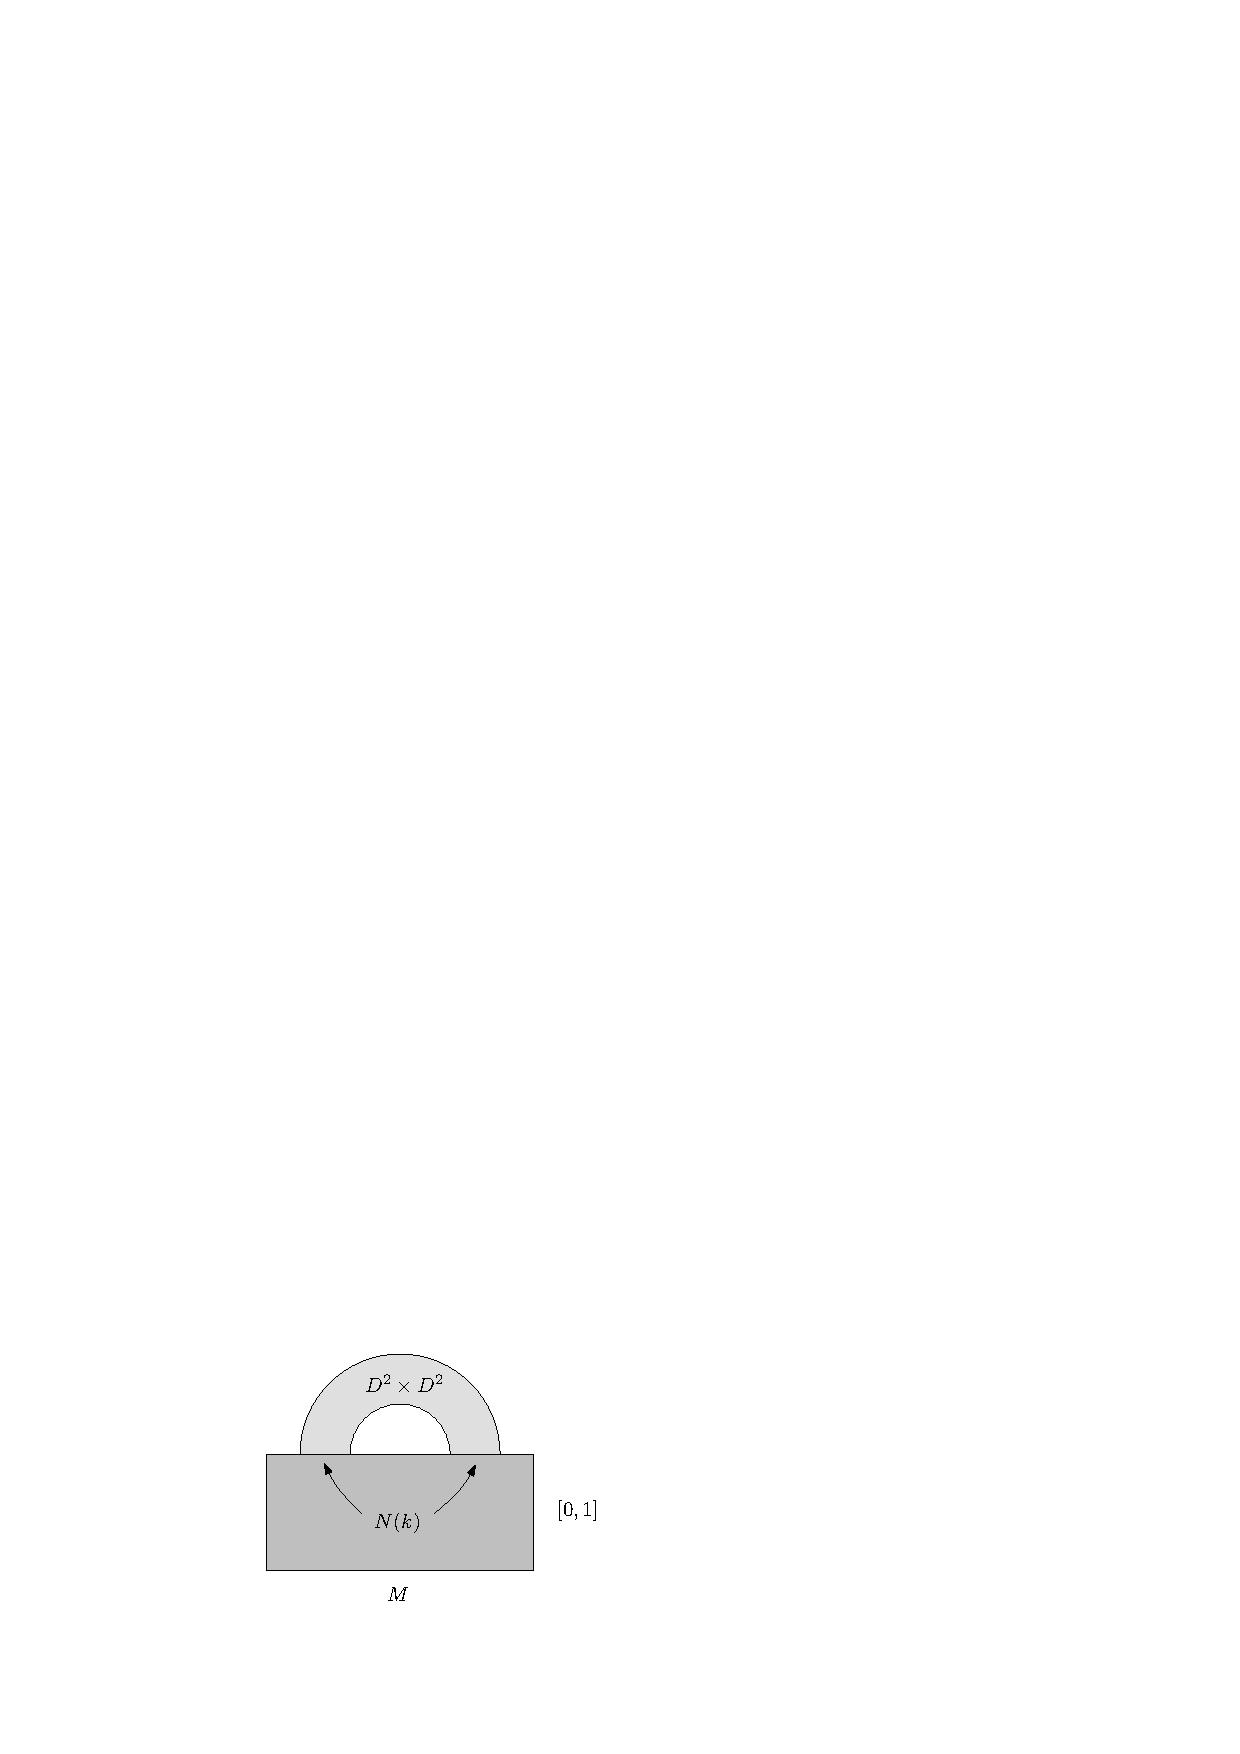
\includegraphics[scale=1.3]{graphics/surgery-cobordism}
\caption{Surgery Cobordism}
\label{surgery cobordism figure}
\end{figure}
\end{proof}

For a framed link $L$, let $W_L$ denote the 4-dimensional cobordism of the surgery on $L$ with zero, i.e. $W_L = $ 0-handle $\cup$ a 2-handle for each component of $L$. This association of a 4-manifold with boundary to any framed link is what allows us to recast Kirby calculus as a 4-dimensional theory. In fact, this is the way Kirby calculus was originally described. The first Kirby move added an unknotted, unlinked component to $L$ with framing $\pm 1$ to get the link $L'$. On the level of 4-manifolds this amounts to $W_{L'}$ being diffeomorphic to $W_L \# \mathbb CP^2$ or $W_L \# \overline{\mathbb CP}^2$, depending on the framing of the added unknot. This follows from \cref{E_n spaces} where we saw that $E_1 = \mathbb CP^2 \backslash D^4$ and $E_{-1} = \overline{\mathbb CP}^2 \backslash D^4$. 

Next, we claim that performing the second Kirby move on two components of $L$ is equivalent to sliding one handle correspond to one component across the handle corresponding to the other component. Since this whole operation is technically taking place in a 4-dimensional manifold it is difficult to picture it. \Cref{sliding-3dim-2handles,sliding-3dim-2handles-2} showed how to slide 3-dimensional 2-handles over each other, and the idea in 4-dimensions is similar. Let us attach two 2-handles $h_1,h_2$ to the 4-ball $D^4$ with attaching circles $k_1,k_2$ and framings $n_1,n_2$ and let $X=D^4\cup h_1\cup h_2$. To slide $h_1$ over $h_2$ we need to find a disc parallel to the core of $h_2$ and then isotope the attaching circle of $h_1$ through this disc. We can take any disc parallel to the core, say $D^2 \times \lcb p \rcb$ where $p \neq 0$. The boundary of this disc is precisely where it intersects the 3-sphere, which is at a longitude $k_2'$ of $k_2$ such that $\lk(k_2,k_2')=n_2$, i.e. its a longitude determined by the framing. As we saw in \cref{sliding-3dim-2handles-2}, isotoping the attaching circle of $h_1$ through this disc is the same as form the banded sum of the attaching circle with the boundary of the disc, so the attaching circle of $h_1$ after sliding across $h_2$ is the connect sum of $k_1$ with $k_2$ along some band disjoint from $k_1$ and $k_2$. We could compute the framing of this handle after the slide directly, or appeal to \cref{intersection form = linking matrix}. Namely, let $\alpha_1,\alpha_2$ be the canonical basis of $H_2(X)$, then after a handle slide this canonical basis has changed to $\alpha_1+\alpha_2,\alpha_2$. The framing on $h_1$ after the slide is
\[ (\alpha_1+\alpha_2)\cdot(\alpha_1+\alpha_2) = \alpha_1\cdot \alpha_1 + \alpha_2\cdot\alpha_2 + 2\alpha_1\cdot\alpha_2 = n_1 + n_2 + 2\lk(k_1,k_2) \]

In \cref{removing unknotted 0-framed components} we saw how an unknotted component with framing 0 that links one other strand exact once allows us to separate and cancel those two components from the rest of the link. What really happened is that we were able to separate the 0-framed unknot and the linked component from the rest of the link, and then we could completely unknot that linked component so that we were left with a Hopf link with one component framed by 0 and the other framed by some integer $n$. By repeatedly sliding handles we arrived at a Hopf link framed by 0 and 0, or 0 and 1 depending on the parity of $n$. The 4-manifolds corresponding to these framed Hopf links are $S^2 \times S^2$ and $S^2 \tilde{\times} S^2$ respectively. So, \cref{removing unknotted 0-framed components} has the following two immediate corollaries.
\begin{cor}
Let $M$ be a 4-dimensional handlebody and let $k_0,k_1$ be attaching circles of two 2-handles such that $k_1$ lies entirely in $\partial D^4$ and $k_0$ is a 0-framed meridian of $k_1$. Finally, let $N$ be the handlebody with all the handles of $M$ except for $k_1$ and $k_2$. Then $M$ is diffeomorphic to $N \# S^2 \times S^2$ if the framing coefficient of $k_1$ is even, and otherwise $M$ is diffeomorphic to $N \# S^2 \tilde{\times} S^2$. 
\end{cor}
\begin{cor}
If $M$ is a 2-handlebody with odd intersection form, then $M \# S^2 \times S^2$ is diffeomorphic to $M \# S^2 \tilde{\times} S^2$.
\end{cor}
\begin{proof}
Since $Q_M$ is odd we must have that any matrix representation of $Q_M$ has an odd number of the diagonal. In particular, if we take the matrix representation with respect to the canonical basis of $H_2(M)$ we see that some 2-handle has odd framing, so let $k$ denote the attaching circle for this handle. Form $M \# S^2 \times S^2$ by adding a Hopf link $\ell_1\cup\ell_2$, both framed as 0, and slide $\ell_1$ over $k$ to obtain $\ell_1'$. Then $\ell_1'$ has odd framing and is linked once by $\ell_2$, so we can separate them from the rest of the link, and reduce it until it is a Hopf link framed by 0 and 1, hence we have $M \# S^2 \tilde{\times} S^2$.
\end{proof}





\comment{
\subsection{Applications}
\label{Applications}

Sometimes we can use Kirby calculus to determine when two 4-dimensional manifolds are diffeomorphic. As we mentioned with Kirby diagrams, once the 1- and 2-handles are attaching in a 4-dimensional handlebody, there is essentially only one way to attach the 3- and 4-handles to get a closed manifold. 

\begin{example}
Recall that $S^2 \times S^2$ is the result of performing a surgery on the 0-framed Hopf link, and then attaching the 4-handle in the only way possible to get a closed manifold. If we introduce an unknotted, unlinked component with framing $+1$ to this Hopf link, the associated 4-manifold is now $(S^2 \times S^2) \# \mathbb CP^2$. By sliding this unknot over a component of the Hopf link, and performing some Kirby calculus we can show that $(S^2 \times S^2) \# \mathbb CP^2$ is diffeomorphic to $\mathbb CP^2 \# \mathbb CP^2 \# \overline{\mathbb CP}^2$, see \cref{s2xs2cp2-cp2cp2cp2}.

\begin{figure}[tb]
\centering
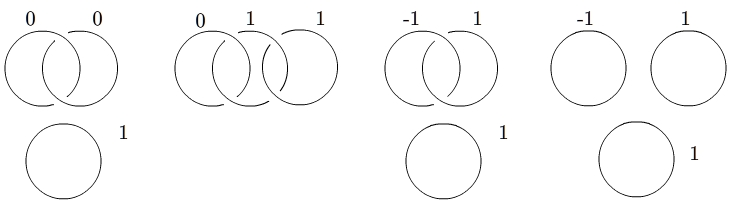
\includegraphics[scale=.6]{graphics/s2xs2cp2-cp2cp2cp2}
\caption{$(S^2 \times S^2) \# \mathbb CP^2 \cong \mathbb CP^2 \# \mathbb CP^2 \# \overline{\mathbb CP}^2$}
\label{s2xs2cp2-cp2cp2cp2}
\end{figure}
\end{example}

\begin{example}
\end{example}
}













\newpage
\section{Morse Homology}
\label{Morse Homology}




\subsection{The Morse-Smale Condition and Moduli Spaces of Flow Lines}
\label{The Morse-Smale Condition and Moduli Spaces of Flow Lines}



Let $f : X \rightarrow \mathbb R$ be a Morse function on a closed, Riemannian $n$-dimensional manifold $(X,\widetilde g)$ with the Levi-Civita connection $\widetilde\nabla$. The metric $\widetilde g$ and connection $\widetilde\nabla$ will be used for background computations, and is not really significant. The set of critical points of $f$ of index $i$ will be denoted by $\crit_i(f)$, and we set $\crit(f)=\cup_i \crit_i(f)$. Recall that at a critical point $p \in \crit(f)$, the tangent space $T_p X$ splits as a direct sum $E^-T_pX \oplus E^+T_pX$, where $E^-T_pX$ and $E^+T_pX$ denote the negative and positive eigenspaces of the Hessian $H_f$ at $p$ and $\dim E^-T_pX = \mu(p)$. A negative gradient flow line is a curve $u : \mathbb R \rightarrow X$ such that $du/dt = -\nabla_g f \circ u$. Since $X$ is compact, $-\nabla_g f$ generates a 1-parameter group of diffeomorphisms $\varphi_t : X \rightarrow X$, i.e $\varphi_t$ is a diffeomorphism for all $t \in \mathbb R$ such that $\varphi_{s+t} = \varphi_s \circ \varphi_t$, $\varphi_0=\id$ and for fixed point $p \in X$ we have 
\[ \frac{d\varphi_t(p)}{dt} = -\nabla_g f(\varphi_t(p)) \]
For a critical point $p \in \crit(p)$ we define the \textbf{ascending} and \textbf{descending manifolds} to be
\[ \mathscr A(p) = \lcb x \in X \st \lim_{t \to \infty}  \varphi_t(x) = p \rcb \]
\[ \mathscr D(p) = \lcb x \in X \st \lim_{t \to -\infty} \varphi_t(x) = p \rcb \]
These sets consist of points that flow to critical points in forward or backward time respectively. The ascending manifold is sometimes called the \textbf{stable} manifold and the descending manifold is sometimes called the \textbf{unstable} manifold. A study of the dynamics of the negative gradient flow allows one to prove the following important statement.
\begin{prop}
\label{ascending and descending manifolds are manifolds}
If $p \in \crit_i(f)$, then $\mathscr D(p)$ and $\mathscr A(p)$ are smoothly embedded discs of dimension $i$ and $n-i$ respectively. Further, $T_p \mathscr D(p) = E^- T_pX$ and $T_p \mathscr A(p) = E^+ T_pX$.
\end{prop}
We will not prove this because it is not useful in our route to defining Morse homology. A pair $(f,g)$ is said to be \textbf{Morse-Smale} if $f$ is a Morse function such that for every pair of critical points $p,q \in \crit(f)$ the ascending and descending manifolds intersect transversely $\mathscr D(p) \pitchfork \mathscr A(q)$. Since codimension is additive under transverse intersections we have $\dim \mathscr D(p) \cap \mathscr A(q) = \mu(p)-\mu(q)$. We do not yet know such pairs even exist (they do, in fact, in abundance), but we immediately get the following lemma.
\begin{lem}
If $(f,g)$ is a Morse-Smale pair on $X$, then a non-constant flow line of $-\nabla_g f$ from $p$ to $q$ has $\mu(p)>\mu(q)$.
\end{lem}
\begin{proof}
Since $(f,g)$ is Morse-Smale we have $\mathscr D(p) \cap \mathscr A(q)$ is a manifold of dimension $\mu(p)-\mu(q)$. If $\mu(p)<\mu(q)$, then this manifold is empty, hence there are no flow lines from $p$ to $q$. If $p=q$, then this is a 0-dimensional manifold whose points correspond to constant flow lines. Therefore if there is a non-constant flow line from $p$ to $q$ we must have $\mu(p)>\mu(q)$.
\end{proof}

\begin{example}
If we stand the torus $T^2$ vertically with the induced metric from its embedding in $\mathbb R^2$, and let $f : T^2 \rightarrow \mathbb R$ be the height function, then $f$ does \emph{not} satisfy the Morse-Smale condition. If we let $p,q,r,s$ denote the critical points of $f$ such that $f(p)>f(q)>f(r)>f(s)$, then we can see that $\mathscr D(q)$ does not intersect $\mathscr A(r)$ transversely. Unfortunately this type of failure of the Morse-Smale condition is common for ``obvious'' choices of Morse functions, which tend to have many symmetries. We can perturb $f$ a little so that it satisfies the Morse-Smale condition (for example, slightly tilt $T^2$ off its vertical axis), but sometimes it is better to consider a more relaxed requirement than Morse-Smale, such as the Morse-Bott condition.
\end{example}

\begin{example}
Consider the flat torus $T^2 = \mathbb R^2 / \mathbb Z^2$ with the smooth function $f : T^2 \rightarrow \mathbb R$ defined by $f(x,y) = \cos(2\pi x) + \cos (2\pi y)$. This function is clearly well defined, and the critical points are at the equivalence classes of $(0,0), (1/2,0), (0,1/2), (1/2,1/2) \in \mathbb R^2$. It is easy to compute the Hessian at these critical points and see that they are non-degenerate, so $f$ is a Morse function. It is also easy to see that all the ascending and descending manifolds intersect transversally, so $f$ satisfies the Morse-Smale condition.
\end{example}

There is another way of discussing the Morse-Smale condition that is better suited for infinite dimensional generalizations of Morse homology. For two critical points $p,q \in \crit(f)$, let $\mathcal M^f(p,q)$ be the moduli space of flow lines from $p$ to $q$, i.e.
\[ \mathcal M^f(p,q) = \lcb u : \mathbb R \rightarrow X \st \frac{du}{dt} = -\nabla_g f(u(t)), u(-\infty)=p, u(\infty)=q \rcb \]
We will show how to put a topology on this set momentarily. This set carries a free $\mathbb R$ action given by pre-composition with translation: $(s \cdot u)(t) = u(t+s)$. Let $\widehat{\mathcal M}^f(p,q)$ denote the quotient of $\mathcal M^f(p,q)$ by this action, which we call the moduli space of unparameterized gradient flow lines. There is an obvious isomorphism between $\mathscr D(p) \cap \mathscr A(q)$ and $\mathcal M^f(p,q)$ as sets since any flow line is uniquely determined by its initial condition, so we would like to know that $\mathcal M^f(p,q)$ is actually a manifold. 

To pursue this we need to develop significant functional analysis machinery. Let $\mathcal C_{p,q}$ be the subset of $W^{1,2}_{loc}(\mathbb R,X)$ such that if $u \in \mathcal C_{p,q}$, then
\begin{enumerate}
	\item $u(-\infty)=p$ and $u(\infty)=q$
	\item There is an $R<0$ sufficiently negative such that $u(-\infty,R]$ is contained in a coordinate chart around $p$ and $u|_{(-\infty,R]} \in W^{1,2}((-\infty,R],X)$.
	\item There is an $R>0$ sufficiently positive such that $u[R,\infty)$ is contained in a coordinate chart around $p$ and $u|_{[R,\infty)} \in W^{1,2}([R,\infty),X)$.
\end{enumerate}
Then $\mathcal C_{p,q}$ is a Banach manifold modeled on $W^{1,2}(\mathbb R,\mathbb R^n)$. Let $\pi_{\mathcal E} : \mathcal E \rightarrow \mathcal C_{p,q}$ be the Banach bundle over $\mathcal C_{p,q}$ defined by
\[ \mathcal E = \bigcup_{u \in \mathcal C_{p,q}} \lcb u \rcb \times L^2(u^* TX) \]
The pullback bundle $u^* TX$ makes sense because the Sobolev embedding $W^{1,2} \hookrightarrow C^0$ ensures that $u$ is continuous, so $\mathcal E$ is a Banach bundle with characteristic fiber $L^2(\mathbb R,\mathbb R^n)$. For any metric $g$ on $X$ we can define a section $F : \mathcal C_{p,q} \rightarrow \mathcal E$ by
\[ F(u) = (u,u'+\nabla_g f \circ u) \]
where $u'$ is the weak derivative of $u$. Technically $F$ depends on the Morse function $f$, metric $g$ and the points $p,q$, but we omit this from the notation. If we let ${0}_{\mathcal E}$ denote the zero section of $\mathcal E \rightarrow \mathcal C_{p,q}$, then we have the following:
\begin{prop}
$F^{-1}({0}_{\mathcal E}) = \mathcal M^f(p,q)$
\end{prop}
\begin{proof}
If $u \in F^{-1}(0_{\mathcal E})$, then $u' = -\nabla_g f \circ u$. Since $\nabla_g f$ and $u$ are continuous, we have $u'$ is continuous, hence $u'$ is equal to the regular derivative $du/dt$. Therefore $u$ is $C^1$ and so is an integral curve from $p$ to $q$, i.e. $u \in \mathcal M^f(p,q)$. On the other hand, if $u \in \mathcal M^f(p,q)$, then $u$ converges exponentially to the critical points $p$ and $q$, so $u \in W^{1,2}(\mathbb R,X)$ and hence $u \in F^{-1}(0_{\mathcal E})$.

By applying the standard bootstrapping argument we see that $u$ is actually as smooth as $g$ (assuming $f$ is smooth), hence $u$ is actually $C^k$.
\end{proof}

In this context we say that $(f,g)$ is a Morse-Smale pair if $F \pitchfork 0_{\mathcal E}$, which of course implies that $\mathcal M^f(p,q)$ is a submanifold of the Banach manifold $\mathcal C_{p,q}$. If we could show that $dF$ is Fredholm at the points in $F^{-1}(0_{\mathcal E})$, then we would have that $F^{-1}(0_{\mathcal E}) = \mathcal M^f(p,q)$ is a finite dimensional submanifold of $\mathcal C_{p,q}$. If we work a little harder we can actually generalize the above constructions a little to show something stronger. Let $\mathcal A^k$ denote the Banach manifold consisting of $C^k$-metrics on $X$. Note that this is just a convex subset of the Banach space (i.e. linear space) of $C^k$ sections of $S^2 T^* X \rightarrow X$. Let $\pi_{\widetilde{\mathcal E}} : \widetilde{\mathcal E} \rightarrow \mathcal A^k \times \mathcal C_{p,q}$ be the Banach bundle that is the pullback of $\mathcal E \rightarrow \mathcal C_{p,q}$ along the projection $\mathcal A^k \times \mathcal C_{p,q} \rightarrow \mathcal C_{p,q}$. In particular, $\widetilde{\mathcal E}$ can be written as
\[ \widetilde{\mathcal E} = \bigcup_{(g,u) \in \mathcal A^k \times \mathcal C_{p,q}} \lcb (g,u) \rcb \times L^2(u^* TX) \]
So, the characteristic fiber of $\widetilde{\mathcal E}$ is $L^2(\mathbb R,\mathbb R^n)$. We define a section $\widetilde F : \mathcal A^k \times \mathcal C_{p,q} \rightarrow \widetilde{\mathcal E}$ of this bundle by $\widetilde F(g,u) = (g,u,u'+\nabla_g f \circ u)$. This section depends only on $f$, but we do not include this in the notation. Then the most important proposition we want to prove is the following.
\begin{prop}
\label{genericity of Morse-Smale metric}
The section $\widetilde{F}$ is transverse to the zero section: $\widetilde{F} \pitchfork 0_{\widetilde{\mathcal{E}}}$. Further, if $\pi : \mathcal A^k \times \mathcal C_{p,q} \rightarrow \mathcal A^k$ is the projection onto the second factor, then the restriction of $\pi$ to $\pi : \widetilde F^{-1}(0_{\widetilde{\mathcal E}}) \rightarrow \mathcal A^k$ is Fredholm of index $\mu(p)-\mu(q)$, i.e. $d\pi_{(g,u)}$ is Fredholm of index $\mu(p)-\mu(q)$ at each $(g,u) \in \widetilde F^{-1}(0_{\widetilde{\mathcal E}})$.
\end{prop}
The immediate corollary of the this proposition is that a generic $g \in \mathcal A^k$ is a regular value of the restricted map $\pi$, hence $\pi^{-1}(g)$ is a finite dimensional submanifold of dimension $\mu(p)-\mu(q)$. Clearly $\pi^{-1}(g) = \mathcal M^f(p,q)$, where this moduli space is taken with respect to $g$, therefore we have the following.
\begin{cor}
The moduli space of flow lines $\mathcal M^f(p,q)$ from $p$ to $q$ for a Morse-Smale pair is a $(\mu(p)-\mu(q))$-dimensional submanifold of $\mathcal C_{p,q}$. The moduli space of unparameterized flow lines $\widehat{\mathcal M}^f(p,q)$ is a $(\mu(p)-\mu(q)-1)$-dimensional manifold.
\end{cor}

\Cref{genericity of Morse-Smale metric} will actually follow reasonably easily from the fact about the vertical differential $DF_u$ of the section constructed for the first Banach bundle $\mathcal E \rightarrow \mathcal C_{p,q}$ is Fredholm.
\begin{prop}
\label{vertical differential is Fredholm}
For each $u \in F^{-1}(0_{\mathcal E})$, the vertical differential $DF_u : T_u \mathcal C_{p,q} \rightarrow \mathcal E_u$ is Fredholm of index $\mu(p)-\mu(q)$.
\end{prop}

So, now we will work to prove \cref{vertical differential is Fredholm}. The first thing we can do is introduce coordinates on our manifolds and bundles so that we can write the vertical differential in a nicer way. To put coordinates on $\mathcal C_{p,q}$ fix $u \in \mathcal C_{p,q}$ and a small open set $U$ around $u$. Let $N(TX)$ be a small enough convex, tubular neighborhood of the zero section of $TX$ so that the exponential map $\exp : N(TX) \rightarrow X$ is defined, where this is the exponential map with respect to the background metric $\widetilde g$ and Levi-Civita connection $\widetilde\nabla$ floating around. This exponential map induces coordinates on $\mathcal C_{p,q}$ in the following way. Let $u \in \mathcal C_{p,q}$ and take another curve $v \in \mathcal C_{p,q}$ close to $u$. Then there is a unique section $\phi(v) \in W^{1,2}(u^* TX)$ (i.e. a $W^{1,2}$ vector field along $u$) such that $v(t) = \exp(u(t),\phi(v)(t))$. So, for a small neighborhood $U$ around $u$ we have a chart $\phi : U \rightarrow W^{1,2}(u^* TX) = T_u \mathcal C_{p,q}$ with $\phi(u)=0$.

\begin{figure}[tb]
\centering
\ \ \ \ \ \ \ \ \ \ \ \ \ \ \ \ \ 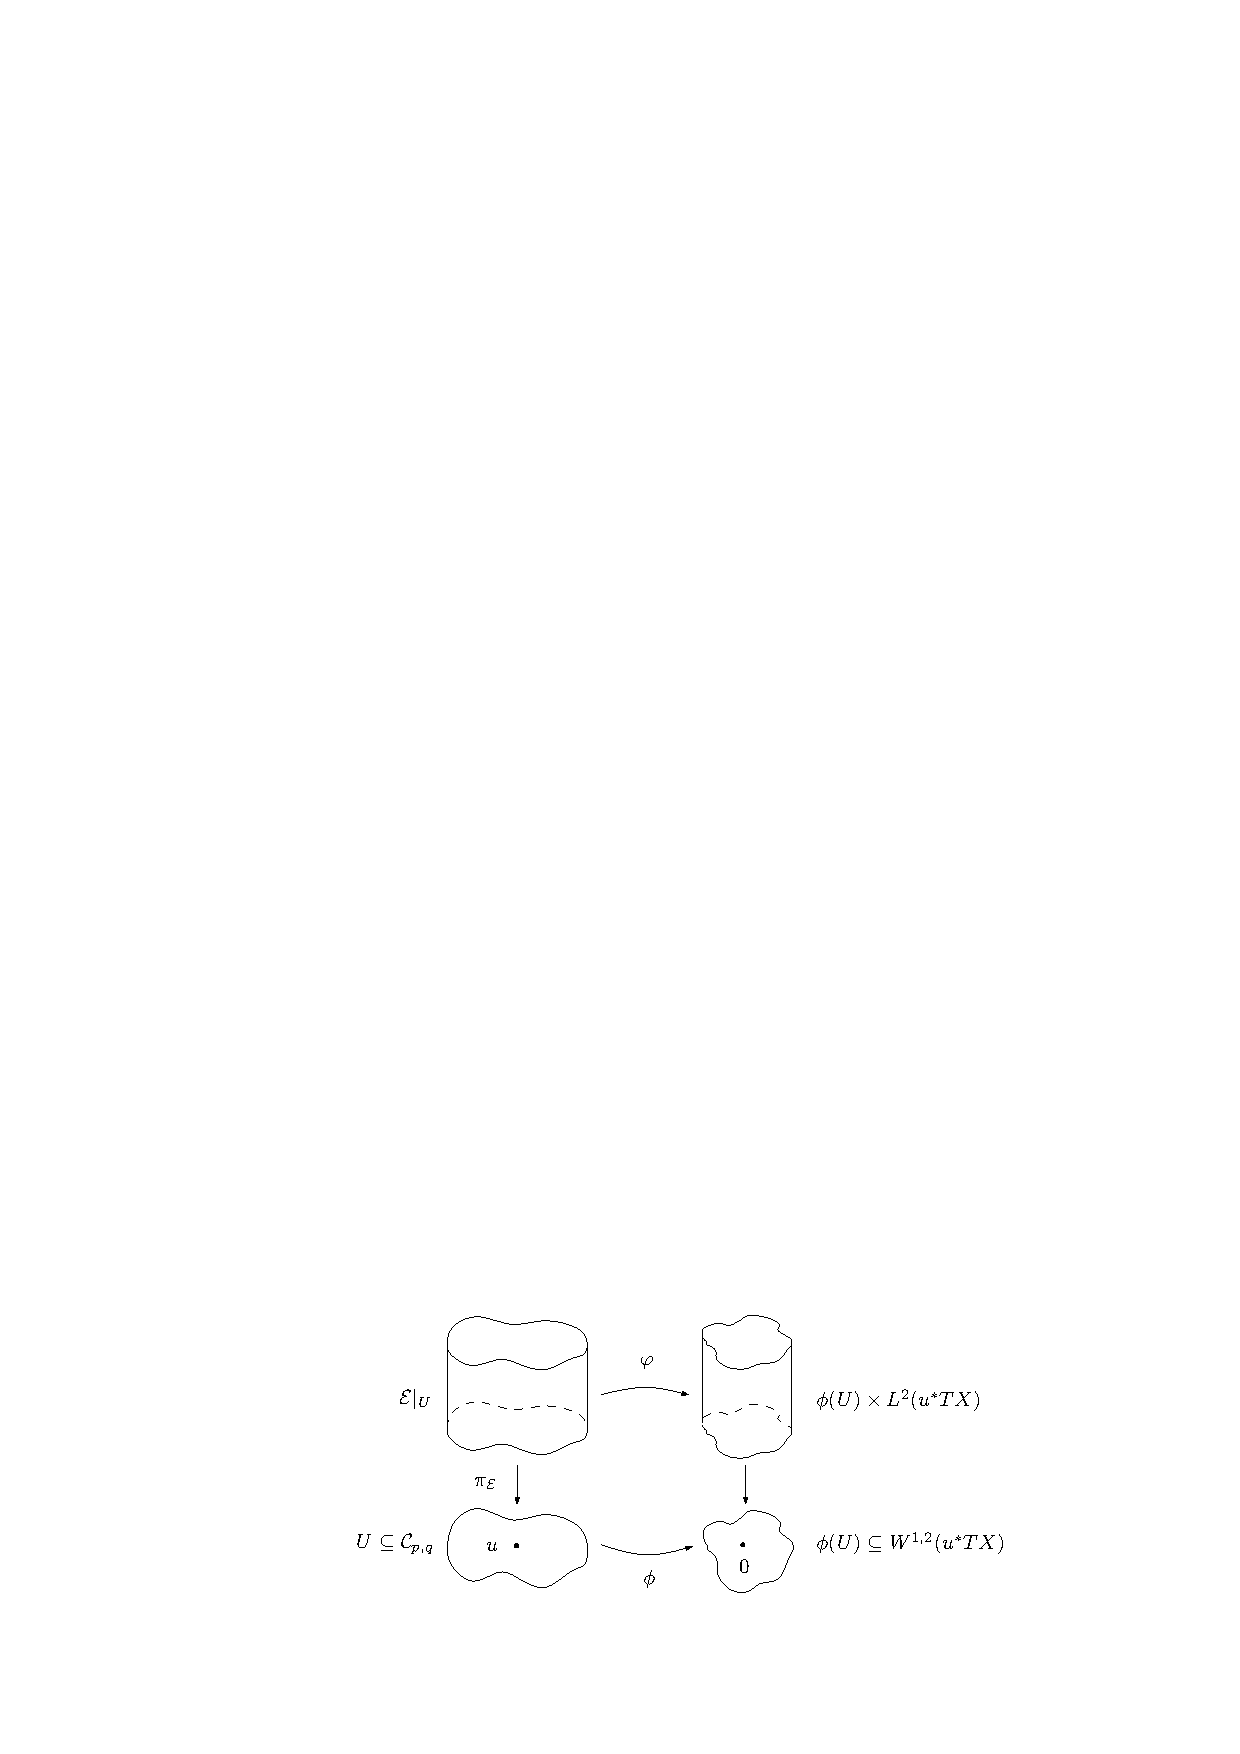
\includegraphics[scale=1]{graphics/banach-bundle}
\caption{Trivializing $\mathcal E \rightarrow \mathcal C_{p,q}$}
\label{banach-bundle}
\end{figure}

Next we trivialize $\pi_{\mathcal E} : \mathcal E \rightarrow \mathcal C_{p,q}$ over $U$. For $v \in U$ we can define the bundle map $P_u^v : u^* TX \rightarrow v^* TX$ that parallel transports a vector $V_t$ in the fiber of $u^* TX$ over $t$ along the geodesic $s \mapsto (u(t),s\phi(v)(t))$ to a vector in the fiber of $v^* TX$ over $t$. This map allows us to identify a section in $L^2(u^* TX)$ with a section in $L^2(v^* TX)$, which are precisely the fibers of $\mathcal E$ over $u$ and $v$. Now that we have coordinates on $(\phi,U)$ around $u$ in $\mathcal C_{p,q}$ and a trivialization of $\mathcal E|_U$ (and hence coordinates on $\mathcal E|_U$), we can write the coordinate representation $F : \phi(U) \rightarrow \phi(U) \times L^2(u^* TX)$ of the section $F$ as
\[ F(\xi) = \left( \xi, (P_u^v)^{-1} \left( \exp(u,\xi)' + \nabla_g f \circ \exp(u,\xi) \right) \right) \]
Computing the vertical differential $DF_u : \phi(U) \rightarrow L^2(u^* TX)$ in these coordinates gives
\begin{align*}
DF_u(\xi)(t) &= \left. \frac{d}{ds} \right|_{s=0} F(s\xi(t)) \\
          &= \left. \frac{d}{ds} \right|_{s=0} \left( (P_u^v)^{-1} \left( \exp(u(t),s\xi(t))' + \nabla_g f(\exp(u(t),s\xi(t)) \right) \right) \\
          &= \widetilde\nabla_{\xi(t)} \left( u'(t) + \nabla_g f(u(t)) \right) \\
          &= \widetilde\nabla_{\xi(t)} u'(t) + \widetilde\nabla_{\xi(t)} \left( \nabla_g f(u(t)) \right) 
\end{align*}
where the second from last line follows from the fact that any connection can be recovered from parallel translations along its geodesics. Also, since the connection is torsion free we have $\widetilde\nabla_{\xi(t)}u'(t) = \widetilde\nabla_{u'(t)} \xi(t)$, so
\[ DF_u(\xi) = \widetilde\nabla_{u'} \xi + \widetilde\nabla_\xi \left( \nabla_g f(u) \right) \]
If we trivialize $u^* TX$ using parallel translation with respect to $\widetilde\nabla$, then vertical differential $DF_u : W^{1,2}(\mathbb R,\mathbb R^n) \rightarrow L^2(\mathbb R,\mathbb R^n)$ can be written as
\[ (DF_u \xi)(t) = \left. \frac{d}{ds} \right|_{s=t} \xi(s) - A_t \xi(t) \]
where $A \in C^k(\mathbb R,\End(\mathbb R^n))$ is defined by $A_t(V)=-\widetilde\nabla_V(\nabla_g f(u(t)))$. By \eqref{connection definition of Hessian} we have
\[ A_{-\infty}=-H_f(p) \ \ \ \ \  A_\infty=-H_f(q) \]
With this set up we will see that \cref{vertical differential is Fredholm} follows from a more general proposition concerning spectral flows (see \cite{rs95}). Before stating this proposition we recall the definition of spectral flow, at least for the special case we need. Let $A \in C_b(\mathbb R,\End(\mathbb R^n))$ be a bounded path of operators on $\mathbb R^n$ such that $A_{\pm\infty}$ are symmetric and do not have zero as an eigenvalue. Then we define the spectral flow of the path $A$ to be the number of eigenvalues of $A_s$ that change from negative to positive as $s$ ranges from $-\infty$ to $\infty$. We denote this integer by $\SF(A)$, and clearly in this special case we have
\[ \SF(A) = \dim E^+(A_\infty) - \dim E^+(A_{-\infty}) \]
\begin{prop}
\label{fundamental spectral flow theorem}
Let $A \in C_b(\mathbb R,\End(\mathbb R^n))$ such that $A_{-\infty}$ and $A_{\infty}$ are symmetric and do not have zero as an eigenvalue. Then the operator $D_A : W^{1,2}(\mathbb R,\mathbb R^n) \rightarrow L^2(\mathbb R,\mathbb R^n)$ given by
\[ D_A \xi = \frac{d}{dt} \xi - A \xi \]
is Fredholm with
\[ \ind D_A = -\SF(A) \]
\end{prop}
\begin{proof}
\end{proof}

Applying \cref{fundamental spectral flow theorem} to the vertical differential $DF_u = d/dt - A_s$ we see that $DF_u$ is Fredholm of index
\begin{align*}
	\ind DF_u &= -\SF(A) \\
	          &= -(\dim E^+(-H_f(q)) - \dim E^+(-H_f(p))) \\
	          &= \dim E^-(H_f(p)) - \dim E^-(H_f(q)) \\
	          &= \mu(p)-\mu(q)
\end{align*}
and this finishes the proof \cref{vertical differential is Fredholm}. Let us see how to use \cref{vertical differential is Fredholm} to prove \cref{genericity of Morse-Smale metric}. 

\begin{proof}[Proof of \cref{genericity of Morse-Smale metric}]
Our derivation of the local expression of the vertical differential $DF_u$ at $u \in F^{-1}(0_{\mathcal E})$ can be slightly adapted to give the following local expression for the vertical differential $D\widetilde F_{(g,u)} : T_{(g,u)} (\mathcal A^k \times \mathcal C_{p,q}) \rightarrow T_{(g,u,0)} \mathcal{\widetilde E}$ at a point $(g,u) \in \widetilde F^{-1}(0_{\widetilde{\mathcal E}})$:
\[ D\widetilde F_u(\eta,\xi) = DF_u(\xi) + \partial_\eta(\nabla_g f(u)) \]
where $\partial_\eta$ denotes the derivative with respect to the $\eta$ variable (remember that $\mathcal A^k$ is just a convex, open subset of a linear space).

Let $(g,u) \in \widetilde F^{-1}(0_{\widetilde{\mathcal E}})$ and consider the differential $d\pi_{(g,u)} : T_{(g,u)} \widetilde F^{-1}(0_{\widetilde{\mathcal E}}) \rightarrow T_g \mathcal A^k$ of the restriction of $\pi$ to $\widetilde F^{-1}(0_{\widetilde{\mathcal E}})$. We claim that the kernel of $d\pi_{(g,u)}$ is isomorphic to the kernel of $DF_u$. We have that
\[ T_{(g,u)} \widetilde F^{-1}(0_{\widetilde{\mathcal E}}) = (D\widetilde F_{(g,u)})^{-1}(T_{(g,u)} 0_{\widetilde{\mathcal E}}) \]
which can be written as
\begin{equation}
\label{tangent space of pre-image of zero section in coordinates}
T_{(g,u)} \widetilde F^{-1}(0_{\widetilde{\mathcal E}}) = \lcb (\eta,\xi) \in T_g \mathcal A^k \oplus T_u \mathcal C_{p,q} \st DF_u(\xi) + \partial_\eta(\nabla_g f(u)) = 0 \rcb 
\end{equation}
using our coordinates. We clearly have $d\pi_{(g,u)}(\eta,\xi) = \eta$, hence
\[ \ker d\pi_{(g,u)} = \lcb (0,\xi) \in T_g \mathcal A^k \oplus T_u \mathcal C_{p,q} \st DF_u(\xi) = 0 \rcb = \ker DF_u \]

Next we claim that the cokernel of $d\pi_{(g,u)}$ is isomorphic to the cokernel of $DF_u$. \todo{do this}.

Finally, we show that the image of $d\pi_{(g,u)}$ is closed. Using our coordinates and \eqref{tangent space of pre-image of zero section in coordinates}, the image of $d\pi_{(g,u)}$ can be written as
\begin{align*}
	d\pi_{(g,u)} \left( T_{(g,u)} \widetilde F^{-1}(0_{\widetilde{\mathcal E}}) \right) &= \lcb \eta \in T_g \mathcal A^k \st DF_u(\xi) + \partial_\eta(\nabla_g f(u)) = 0 \text{ for some } \xi \in T_u \mathcal C_{p,q} \rcb \\
	&= \lcb \eta \in T_g \mathcal A^k \st \partial_\eta (\nabla_g f(u)) \in \image DF_u \rcb
\end{align*}
So, we see that $\image d\pi_{(g,u)}$ is the pre-image of $\image DF_u$ under the map $\eta \mapsto \partial_\eta(\nabla_g f(u))$. This map is continuous, and $DF_u$ is closed since it is Fredholm, therefore $\image d\pi_{(g,u)}$ is closed.
\end{proof}





\begin{prop}
A generic $C^k$ function $f : X \rightarrow \mathbb R$ ($k \geq 2$) is Morse.
\end{prop}
\begin{proof}
We clearly want to use the Sard-Smale theorem somehow, and in fact we will use \cref{useful Banach bundle result}. In order to use this we need to formulate a Banach bundle such that the zero section corresponds to what we want. In particular, let $\pi : \mathcal F \rightarrow C^k(X) \times X$ be the Banach bundles that is the pullback of the cotangent bundle $T^* X \rightarrow X$ along the projection $C^k(X) \times X \rightarrow X$ so that the fiber of $\mathcal F$ over $(f,p)$ is just $T_x^* X$. Consider the section $s : C^k(X) \times X \rightarrow \mathcal F$ given by $s(f,p) = df_p \in T_p^* X$. Let $(f,x) \in \pi^{-1}(0_{\mathcal F})$ and let us compute the vertical differential $Ds_{(f,x)} : T_{(f,x)} (C^k(X) \times X) \rightarrow T_x^*X$ at $(f,x)$. Note that since $C^k(X)$ is a linear space we have $T_f C^k(X)$ is naturally isomorphic to $C^k(X)$, so we describe how $Ds_{(f,x)}$ acts on a pair $(h,V) \in C^k(X) \times T_x X$.
\[ Ds_{(f,p)}(h,V) = dh(X) + \nabla_V(df) \]

\unfinished
\end{proof}




\subsection{The Compactness and Gluing Theorems}
\label{The Compactness and Gluing Theorems}

The space of unparameterized flow lines $\widehat{\mathcal M}^f(p,q)$ is not always compact; for example, in \cref{broken-flow-line-example} we see a sequence of flow lines (the thin curves) on the deformed sphere that converge to a ``broken'' curve (the bolded curve). A \textbf{broken flow line} from $p$ to $q$ is a sequence of critical points $r_1=p,r_2,\ldots,r_{k-1},r_k=q \in \crit(f)$ and curves $\gamma_1,\ldots,\gamma_{k-1}$ in $X$ such that $\gamma_i$ is a flow line from $r_i$ to $r_{i+1}$. However, there is a canonical compactification of $\widehat{\mathcal M}^f(p,q)$ to a manifold with corners by adding ``broken'' flow lines. There are two parts to this compactification process. The first part (called the compactness result) consists of identifying how a sequence can fail to converge in $\widehat{\mathcal M}^f(p,q)$, trying to get a reasonable object out of a diverging sequence, and then adding these points to $\widehat{\mathcal M}^f(p,q)$ to get a compact space. The second part (called the gluing result) consists of showing that a broken flow line can be slightly perturbed to an honest flow line so that our compactification is a manifold with corners.

\begin{figure}[tb]
\centering
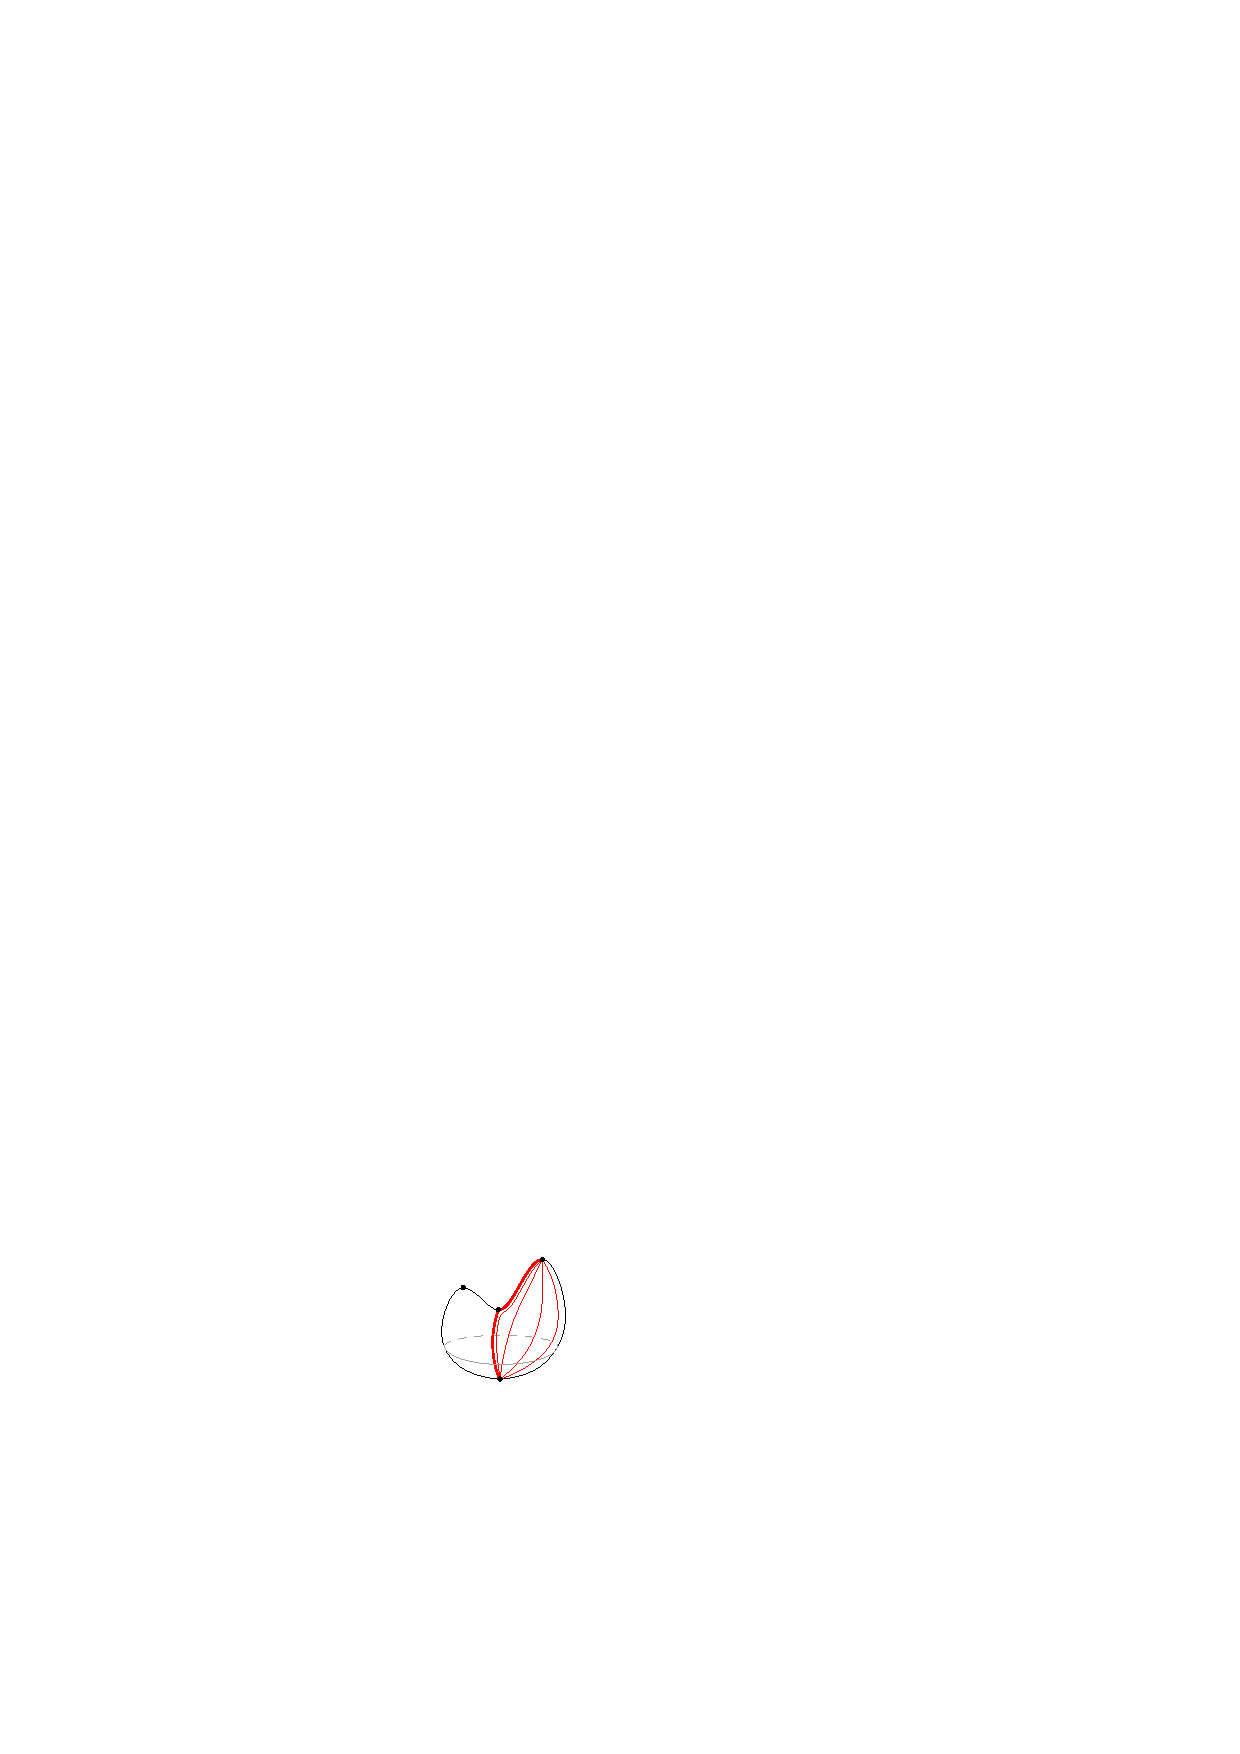
\includegraphics[scale=2]{graphics/broken-flow-line-example}
\caption{Flow lines converging to a broken flow line}
\label{broken-flow-line-example}
\end{figure}

Recall that a second countable, Hausdorff space $X$ is said to be a \textbf{smooth $n$-manifold with corners} if every point $x \in X$ has an open neighborhood $U_\alpha$ and homeomorphism $\varphi_\alpha : U_\alpha \rightarrow \mathbb R^{n-k} \times [0,\infty)^k$ (for some $0 \leq k \leq n$) such that the transition functions $\varphi_\beta \circ \varphi_\alpha^{-1}$ are smooth. For $0 \leq k \leq n$, we define the \textbf{codimension $k$ stratum} of $X$ to be the set $X_k$ of points $x \in X$ with a chart $\varphi : U \rightarrow \mathbb R^{n-k} \times [0,\infty)^k$ such that at least one of the last $k$ coordinates of $\varphi(x)$ is zero. Note that $X_0$ is just the interior of $X$, and if $X_2=X_3=\cdots=X_n=\emptyset$, then $X$ is just a manifold with boundary and $X_1 = \partial X$. So we will use the notation $\partial X$ to denote $X_1$ even when the higher strata are non-empty.

Now we look at what it means for a sequence in $\widehat{\mathcal M}^f(p,q)$ to converge, and how this convergence can fail. In $\mathcal M^f(p,q)$, a sequence of elements converges if it converges in the subspace topology induced by the Banach manifold $\mathcal C_{p,q}$. Since modding out by the $\mathbb R$ action identifies flow lines that differ by only a translation we have that a sequence $(\widehat{u}_n)$ of unparameterized flow lines in $\widehat{\mathcal M}^f(p,q)$ converge to a flow line $\widehat{u}$ if for any sequence of lifts $(u_n)$ of $(\widehat{u}_n)$ and lift $u$ of $\widehat{u}$ there is a sequence $(s_n)$ of real numbers such that $s_n \cdot u_n$ converges to $u$ in $\mathcal M^f(p,q)$.

\todo{finish compactifications and gluing}





-- -- -- -- -- -- -- -- -- 

The BIG theorem:
\begin{thm}
\label{compactification of the moduli space of unparameterized flow lines}
If $X$ is a closed $n$-manifold and $(f,g)$ is a Morse-Smale pair, then for any two critical points $p,q$, the manifold $\widehat{\mathcal M}^f(p,q)$ has a natural compactification to a smooth manifold with corners $\overline{\widehat{\mathcal M}^f(p,q)}$ whose codimension $k$ stratum is
\[ \overline{\widehat{\mathcal M}^f(p,q)}_k = \bigcup_{\scriptsize\begin{array}{c} r_1,\ldots,r_k \in \crit(f) \\ p,r_1,\ldots,r_k,q \text{ distinct} \end{array}} \widehat{\mathcal M}^f(p,r_1) \times \widehat{\mathcal M}^f(r_1,r_2) \times \cdots \widehat{\mathcal M}^f(r_{k-1},r_k) \times \widehat{\mathcal M}^f(r_k,q) \]
In particular, if $k=1$, then as oriented manifolds we have
\[ \partial \overline{\widehat{\mathcal M}^f(p,q)} = \bigcup_{\scriptsize\begin{array}{c} r \in \crit(f) \\ p,r,q \text{ distinct} \end{array}} (-1)^{\mu(p)+\mu(r)+1} \widehat{\mathcal M}^f(p,r) \times \widehat{\mathcal M}^f(r,q) \]
\end{thm}

The two most important special cases of this theorem are when $\mu(q)=\mu(p)-1$, in which case $\mathcal M^f(p,q)$ is a compact 0-manifold (hence a finite collection of points), and when $\mu(q)=\mu(p)-2$, in which case $\widehat{\mathcal M}^f(p,q)$ has a compactification to a 1-manifold with boundary $\overline{\widehat{\mathcal M}^f(p,q)}$ such that $\partial\overline{\widehat{\mathcal M}^f(p,q)}$ consists of just once broken flow lines:
\[ \partial \overline{\widehat{\mathcal M}^f(p,q)} = \bigcup_{r \in \crit_{\mu(p)-1}(f)} \widehat{\mathcal M}^f(p,r) \times \widehat{\mathcal M}^f(r,q) \]








\subsection{The Morse Complex}
\label{The Morse Complex}


We can now define the \textbf{Morse complex}\footnote{Some might call this construction the Morse-Smale-Witten complex due to its complicated history. See \cite{bott1988} for the interesting history of Morse theory and Morse homology} associated to a Morse-Smale pair $(f,g)$. Let $CM_i(f,g)$ be the $\mathbb Z/2$ vector space generated by the critical points of index $i$
\[ CM_i(f,g) := \bigoplus_{p \in \crit_i(f)} \mathbb Z/2 \< p\> \]
We can define this complex with $\mathbb Z$ coefficients if we work harder and define orientations on the moduli spaces $\mathcal M^f(p,q)$. It is simpler to work with $\mathbb Z/2$ coefficients for now, and we will discuss orientation issues later. The differential $\partial : CM_i(X) \rightarrow CM_{i-1}(X)$ counts the number of flow lines between critical points. Specifically, if $p \in \crit_i(f)$, then
\[ \partial(p) = \sum_{q \in \crit_{i-1}(f)} \# \widehat{\mathcal M}^f(p,q) \cdot q \]
and extend linearly to $CM_i(f)$. The count $\# \widehat{\mathcal M}^f(p,q)$ is of course done modulo 2 (at least until we can define orientations).

\begin{prop}
\label{Morse differential}
$\partial \circ \partial = 0$
\end{prop}
\begin{proof}
First recall that the number of points in the boundary of a 1-manifold is zero when counted modulo 2. For $p \in \crit_i(f)$ we can easily compute
\begin{align*}
	\partial \circ \partial (p) &= \partial \left( \sum_{r \in \crit_{i-1}(f)} \# \mathcal M^f(p,r) \cdot r \right) \\
	                            &= \sum_{r \in \crit_{i-1}(f)} \# \mathcal M^f(p,r) \cdot \partial (r) \\
                                &= \sum_{q \in \crit_{i-2}(f)} \left( \sum_{r \in \crit_{i-1}(f)} \# \mathcal M^f(p,r) \cdot \# \mathcal M^f(r,q) \right) \cdot q
\end{align*}
So, the coefficient of $q \in \crit_{i-2}(f)$ in $\partial \circ \partial(p)$ is precisely $\# \partial \overline{\mathcal M^f(p,q)}$, which is zero since it is a compact 1-dimensional manifold.
\end{proof}

We define the \textbf{Morse homology} $HM_*(f,g)$ of the pair $(f,g)$ to be the homology of the chain complex $(CM_*(f,g),\partial)$. 






\subsection{A Natural Isomorphism between Morse and Singular Homology}
\label{A Natural Isomorphism between Morse and Singular Homology}


We would like to show that the homology groups do not depend on our choice of Morse function or metric. There are many ways of doing this, but the first way we will consider is to show that $HM_*(f,g)$ is naturally isomorphic to some other known homology theory, such as singular homology, which of course implies that $HM_*(f,g)$ does not depend on $f$ or $g$.

The homology theory we will show is naturally isomorphic to $HM_*$ is defined as follows. Recall that an \textbf{$i$-dimensional current} on $X$ is a functional on the space of differential $i$-forms $\Omega^i(X)$. The topology on $\Omega^i(X)$ is defined by saying that a sequence of differential forms $\lcb \omega_n \rcb$ converges to $\omega$ if and only if for every compact set $K \subseteq X$ all partial derivatives of $\omega_n$ (in any coordinate system) converges uniformly to the partial derivatives of $\omega$. A singular simplex $\sigma : \Delta^i \rightarrow X$ determines an $i$-dimensional current $[\sigma]$ by 
\[ [\sigma](\omega) = \int_{\Delta^i} \sigma^* \omega \]

\comment{
An $n$-dimensional manifold $X$ carries a natural $n$-dimensional current, called the \textbf{fundamental current} and denoted by $[X]$, that is defined by
\[ [X](\omega) = \int_X \omega \]
}

We define the chain groups $C_i^c(X)$ of our homology theory to be the free abelian group generated by $[\sigma]$, where $\sigma : \Delta^i \rightarrow X$ is a singular $i$-simplex that is transverse to $\mathscr A(p)$ for all $p \in \crit(f)$. The differential $\partial : C_i^c(X) \rightarrow C_{x-1}^c(X)$ is defined by
\[ \partial [\sigma] (\omega) = \int_{\Delta^i} \sigma^* d\omega \]
where $\sigma \in C_i(X)$ and $\omega \in \Omega^{i-1}(X)$. We clearly have $\partial^2=0$ since $d^2=0$. The homology of this chain complex will be denoted by $H_i^c(X)$, and it is naturally isomorphic to singular homology. 

There is a natural compactification of $\mathscr D(p)$, for $p \in \crit(f)$, that is similar to \cref{compactification of the moduli space of unparameterized flow lines} by adding broken flow lines.
\begin{prop}
There is a natural compactification of $\mathscr D(p)$ to a smooth manifold with corners $\overline{\mathscr D(p)}$, whose codimension $k$ stratum is
\[ \overline{\mathscr D(p)}_k = \bigcup_{\scriptsize\begin{array}{c} q_1,\ldots,q_k \in \crit(f) \\ p,q_1,\ldots,q_k \text{ distinct} \end{array}} \widehat{\mathcal M}^f(p,q_1) \times \widehat{\mathcal M}^f(q_1,q_2) \times \widehat{\mathcal M}^f(q_{k-1},q_k) \times \mathscr D(q_k) \]
In particular, for $k=1$ we have
\[ \partial\overline{\mathscr D(p)} = \bigcup_{p \neq q \in \crit(f)} (-1)^{\mu(p)+\mu(q)+1} \widehat{\mathcal M}^f(p,q) \times \mathscr D(q) \]
as oriented manifolds. Further, the projections of $\overline{\mathscr D(p)}$ onto the last factor $\mathscr D(q_k)$ patch together to form a smooth map $e : \overline{\mathscr D(p)} \rightarrow X$ whose restriction to $\mathscr D(p)$ is the inclusion.
\end{prop}

The compactified spaces $\overline{\mathscr D(p)}$ are homeomorphic to a closed ball of dimension $\mu(p)$, and so the maps $e : \overline{\mathscr D(p)} \rightarrow X$ give $X$ a CW-structure with one cell of dimension $i$ for each critical point of index $i$. A consequence of this is that $\chi(X)$ is equal to $\sum_i (-1)^i c_i$ where $c_i = \# \crit_i(f)$.

We now define maps $D : CM_i(X) \rightarrow C_i^c(X)$ and $A : C_i^c(X) \rightarrow CM_i(X)$ that are chain homotopy inverses of each other. For $p \in \crit_i(f)$ we have $\overline{\mathscr D(p)}$ is a closed disc of dimension $i$.


\unfinished




\subsection{Direct Invariance of Morse Homology}
\label{Direct Invariance of Morse Homology}


Now we will show that $HM_*(f,g)$ does not depend on $f$ and $g$ directly. This line of reasoning is more applicable to Floer homologies than \cref{A Natural Isomorphism between Morse and Singular Homology} since there might not be another well-known homology theory to compare to. Fix two Morse-Smale pairs $(f_0,g_0)$ and $(f_1,g_1)$ with associated Morse complexes $(C_*^0,\partial^0)$ and $(C_*^1,\partial^1)$. Take any path of pairs $\Gamma = \lcb (f_t,g_t) \st t \in I \rcb$ from $(f_0,g_0)$ to $(f_1,g_1)$. Two things to note: the pairs $(f_t,g_t)$ do not have to be Morse-Smale for all $t$ (in fact, it may be impossible), and such a path is always possible as all functions $M \rightarrow \mathbb R$ are homotopic and any two metrics can be connected by a straight line of metrics. We will show how such a path (with some simple requirements) induces a chain map $\Phi_\Gamma : C_*^0 \rightarrow C_*^1$. 

Let $V_t$ denote the negative gradient vector field of $f_t$ with respect to $g_t$, and define the vector field $V_\Gamma$ on $I \times X$ by
\begin{equation}
\label{path of pairs vector field}
V_\Gamma = (t+1)t(t-1) \pfrac{}{t} + V_t
\end{equation}
Since the two components of this vector field are gradient like vector fields, we can define critical points, flow lines, ascending and descending manifolds in the regular way. In particular, the first coordinate of $V_\Gamma$ is just the gradient of the function $\mathbb R \rightarrow \mathbb R$ defined by $t \mapsto \frac{1}{4}(t+1)^2(t-1)^2$. This function only has critical points at $-1,0,1$ of index $0,1,0$ respectively. Thus, the critical points of index $i$ of $V_\Gamma$ are precisely
\begin{equation}
\label{critical points of V}
\crit_i(V_\Gamma) = \lcb 0 \rcb \times \crit_{i-1}(f_0) \cup \lcb 1 \rcb \times \crit_i(f_1)
\end{equation}
We will say that the path $\Gamma$ is \textbf{admissible} if the ascending and descending manifolds of the critical points of $V_\Gamma$ intersect transversely. Just as almost all pairs $(f,g)$ are Morse-Smale we also have that almost all paths of pairs are admissible.

For critical points $P,Q$ of $V_\Gamma$ we define $\mathcal M^\Gamma(P,Q)$ to be the moduli space of flow lines of $V_\Gamma$ from $P$ to $Q$, and $\widehat{\mathcal M}^\Gamma(P,Q)$ the moduli space of unparameterized flow lines. If $\Gamma$ is admissible, then $\mathcal M^\Gamma(P,Q)$ is a $(\mu(P)-\mu(Q))$-dimensional manifold, and so $\widehat{\mathcal M}^\Gamma(P,Q)$ is a ($\mu(P)-\mu(Q)-1$)-dimensional manifold. The spaces $\widehat{\mathcal M}^\Gamma(P,Q)$ are without boundary, but are not generally compact. We can compactify them via broken lines as before. We state this result only for the two special cases we need. If $\mu(P)=\mu(Q)+1$, then $\widehat{\mathcal M}^\Gamma(P,Q)$ is already compact, and since it is 0-dimensional we have that it is just a finite collection of points. If $\mu(p)=i=\mu(q)+1$, then $\mu((0,p))=i+1$ and $\mu((1,q))=i-1$, then $\widehat{\mathcal M}^\Gamma((0,p),(1,q))$ is a 1-dimensional manifold with a compactification $\overline{\widehat{\mathcal M}^\Gamma((0,p),(1,q))}$ by adding broken flow lines that pass through one intermediate critical points of index $i$. These points correspond to \cref{critical points of V}, and so we have
\begin{align*}
\partial \overline{\widehat{\mathcal M}^\Gamma((0,p),(1,q))} &= \bigcup_{r \in \crit_{i-1}(f_0)} \widehat{\mathcal M}^\Gamma((0,p),(0,r)) \times \widehat{\mathcal M}^\Gamma((0,r),(1,q)) \\
 &= \bigcup_{r' \in \crit_i(f_1)} \widehat{\mathcal M}^\Gamma((0,p),(1,r')) \times \widehat{\mathcal M}^\Gamma((1,r'),(1,q))
\end{align*}
Note that a flow line between two points in the $\lcb 0 \rcb \times X$ slice must stay in that slice for all time, and similarly for the $\lcb 1 \rcb \times X$ slice. The flow lines in the these slices correspond to the flows of $f_0$ and $f_1$ in $X$, so we have
\[ \widehat{\mathcal M}^\Gamma((0,p),(0,r)) = \widehat{\mathcal M}^{f_0}(p,r) \]
\[ \widehat{\mathcal M}^\Gamma((1,r'),(1,q)) = \widehat{\mathcal M}^{f_1}(r',q) \]

For $p \in \crit_i(f_0)$ and $q \in \crit_i(f_1)$ we have $\mu((0,p))=i+1$ and $\mu((0,q))=i$, hence $\widehat{\mathcal M}^\Gamma((0,p),(1,q))$ is a compact 0-dimensional manifold. We now define $\Phi_\Gamma : C_i^0 \rightarrow C_i^1$ on $p \in \crit_i(f_0)$ by
\[ \Phi_\Gamma(p) = \sum_{q \in \crit_i(f_1)} \# \widehat{\mathcal M}^\Gamma((0,p),(1,q)) \cdot q \]
and extend this linearly to all of $C_*^0$ (where $\widehat{\mathcal M}^\Gamma((0,p),(1,q))$ is counted modulo 2).

\begin{prop}
$\Phi_\Gamma$ is a map of chain complexes, i.e. the following diagram commutes
\[
\xymatrix
@R=2.5PC
@C=2.5PC
{
	C_i^0 \ar[r]^{\partial^0} \ar[d]_{\Phi_\Gamma} & C_{i-1}^0 \ar[d]^{\Phi_\Gamma} \\
	C_i^1 \ar[r]_{\partial^1} & C_{i-1}^1 
}
\]
\end{prop}
\begin{proof}
We will use the idea from the proof of \cref{Morse differential} by showing the coefficient of $q \in \crit_i(f_1)$ in $(\Phi_\Gamma \circ \partial^0 - \partial^1 \circ \Phi_\Gamma)(p)$ is equal to a count of the number of boundary components of a compact 1-manifold, and hence is zero (modulo 2).

For $p \in \crit_i(f_0)$ we have
\begin{align}
\label{chain map differential compositions}
\begin{array}{rl}
	\Phi_\Gamma \circ \partial^0(p) &= \displaystyle \sum_{r \in \crit_{i-1}(f_0)} \sum_{q \in \crit_{i-1}(f_1)} \# \widehat{\mathcal M}^{f_0}(p,r) \cdot \# \widehat{\mathcal M}^\Gamma((0,r),(1,q)) \cdot q \\
	\partial^1 \circ \Phi_\Gamma(p) &= \displaystyle \sum_{r' \in \crit_i(f_1)} \sum_{q \in \crit_{i-1}(f_1)} \# \widehat{\mathcal M}^\Gamma((0,p),(1,r')) \cdot \# \widehat{\mathcal M}^{f_1}(r',q) \cdot q
\end{array}
\end{align}
Now it is clear that the coefficient of $q \in \crit_{i-1}(f_1)$ in $(\Phi_\Gamma \circ \partial^0 - \partial^1 \circ \Phi_\Gamma)(p)$ is precisely the number of boundary components in the compact 1-manifold $\overline{\widehat{\mathcal M}^\Gamma((0,p),(1,q))}$, hence zero. Therefore $\Phi_\Gamma$ is a chain map.

\begin{figure}[tb]
\centering
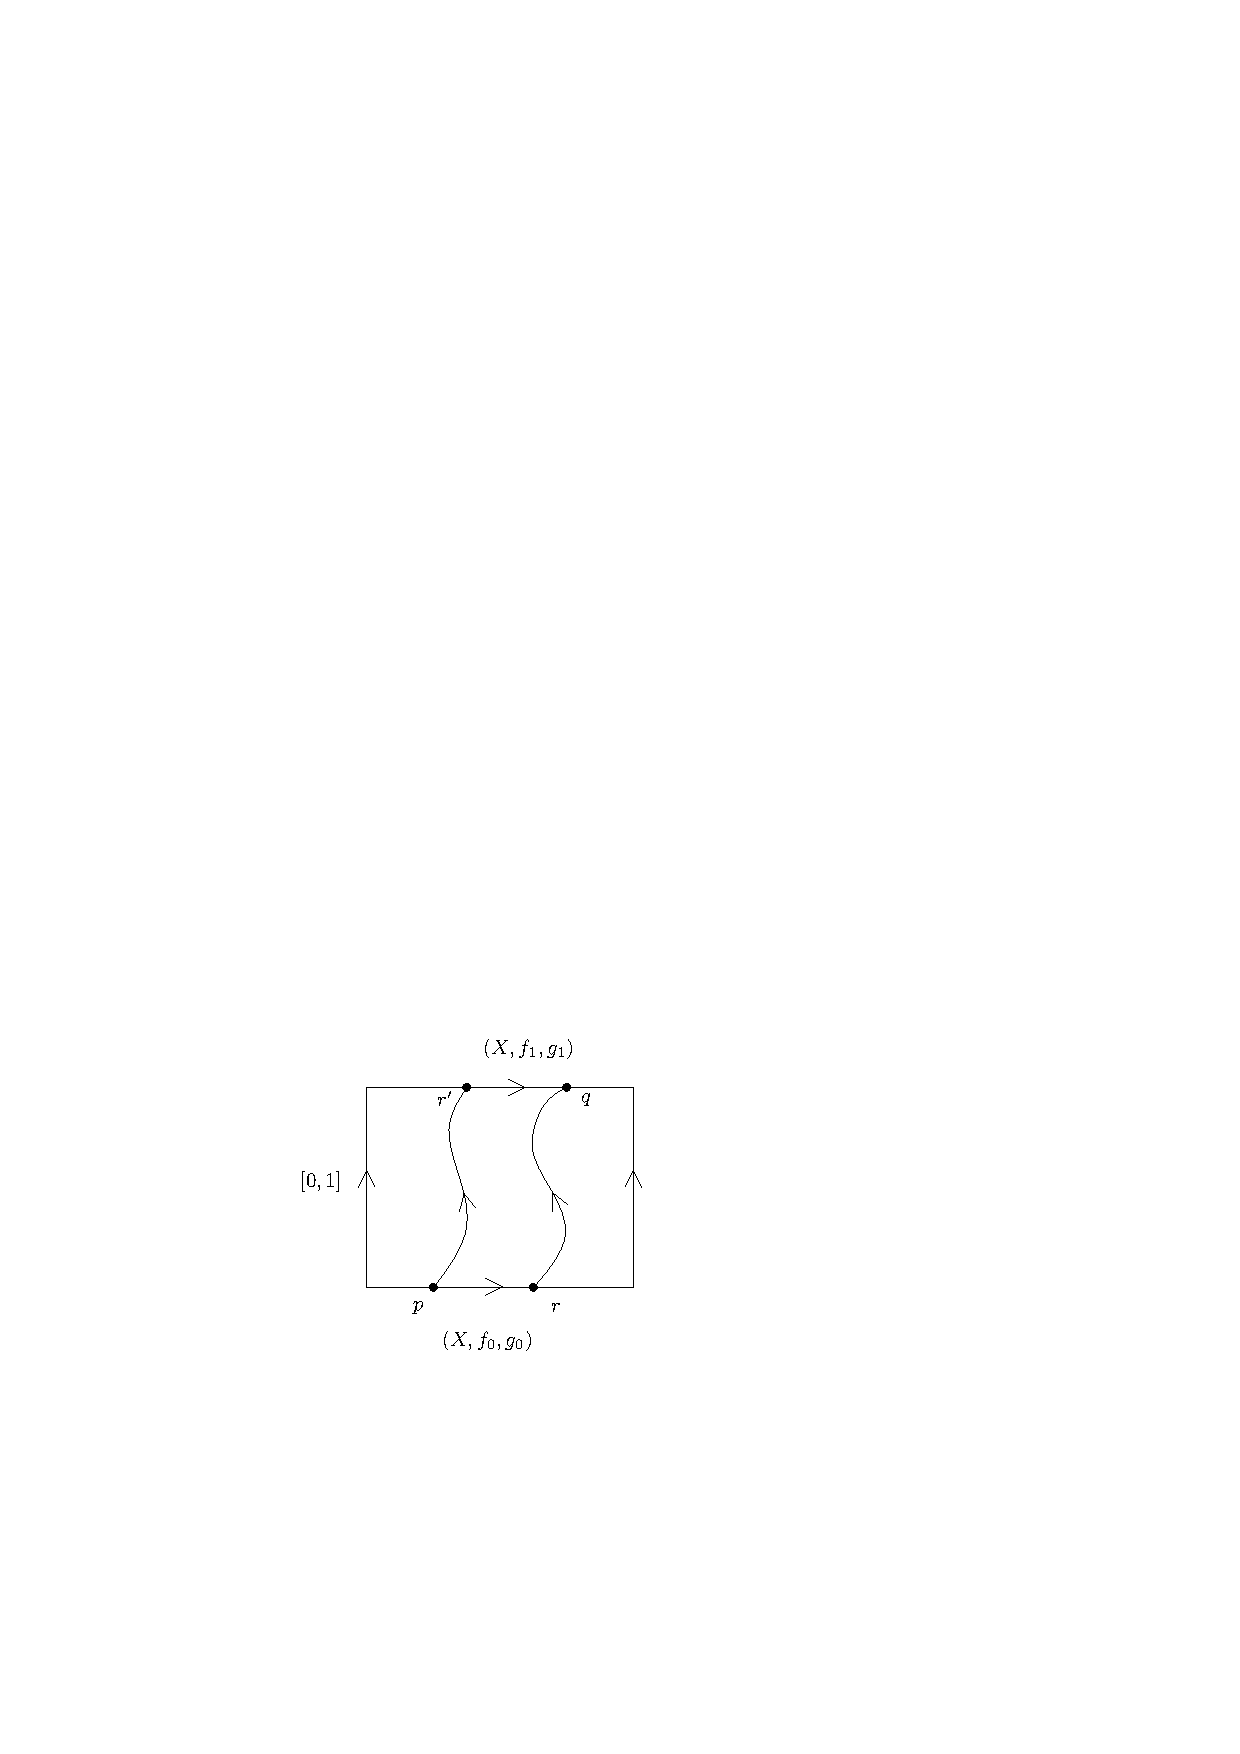
\includegraphics[scale=1]{graphics/path-of-pairs-vector-field}
\caption{Counting flow lines from $(0,p)$ to $(1,q)$}
\label{path-of-pairs-vector-field}
\end{figure}
\end{proof}

We now have that admissible paths $\Gamma$ induce maps on Morse homology $\Phi_{\Gamma*} : HM_*(f_0,g_0) \rightarrow HM_*(f_1,g_1)$. If we take $\Gamma$ to be the constant path at a Morse-Smale pair $(f,g)$, then we expect the induced map $\Phi_\Gamma$ to be the identity. This is indeed the case, as is shown in the following proposition.
\begin{prop}
\label{constant path induces identity}
Let $\Gamma$ be the constant path at the Morse-Smale pair $(f,g)$. Then $\Gamma$ is admissible and $\Phi_\Gamma = \id$
\end{prop}
\begin{proof}
Let $V$ be the vector field on $[0,1] \times X$ induced by the constant path $\Gamma$, i.e. $V = (t+1)t(t-1) \pfrac{}{t} - \nabla_g f$. Since the vector field $(t+1)t(t-1) \pfrac{}{t}$ on $[0,1]$ is directed from 0 to 1, we have that the descending manifold of a critical point $(0,p)$ of $V$ is $\mathscr D(0,p)=[0,1) \times \mathscr D(p)$ and the ascending manifold of a critical point $(1,q)$ is $\mathscr A(1,q) = (0,1] \times \mathscr A(q)$. These submanifolds clearly intersect transversally. On the other hand, the ascending manifold of $(0,p)$ is just $\lcb 0 \rcb \times \mathscr A(p)$ and the descending manifold of $(1,q)$ is just $\lcb 1 \rcb \times \mathscr D(q)$, which do not intersect at all. Therefore $V$ is admissible.

For $p,q \in \crit_i(f)$, a flow from $(0,p)$ to $(1,q)$ in $[0,1] \times X$ projects to a flow from $p$ to $q$ in the $\lcb 0 \rcb \times X$ slice. This implies $p=q$ since there are no flows between critical points of equal index, unless it is the constant flow. Therefore $\Phi_\Gamma(p)=p$.
\end{proof}

Next, we would like to know that $\Phi_\Gamma$ depends only on the homotopy type of the path $\Gamma$. We will use a different model for homotopies than the typical 1-parameter family of maps. Let $D$ be a 2-dimensional manifold with corners such that $D$ has two edges, call them $e$ and $e'$, and two vertices, call them $v$ and $w$. Such a space is sometimes called a \textbf{digon}. If $\Gamma_1,\Gamma_2$ are two paths between pairs $(f_0,g_0)$ and $(f_1,g_1)$, then a homotopy is just a family of pairs $\Psi = \lcb (f_d,g_d) \st d \in D \rcb$ such that when restricted to $e$ it coincides with $\Gamma_1$ and when restricted to $e'$ it coincides with $\Gamma_2$. This means that $(f_v,g_v)=(f_0,g_0)$ and $(f_w,g_w)=(f_1,g_1)$.

Put a metric $\widetilde g$ on $D$ such that the length of the edges is 1, and let $\widetilde f : D \rightarrow \mathbb R$ be a smooth function with only two critical points, one at $v$ of index 2 and one at $w$ of index 0. Further, assume that the negative gradient vector field $\widetilde V = -\nabla_{\widetilde g} \widetilde f$ with respect to $\widetilde g$ is tangent to the edges and is equal to $(t+1)t(t-1)$ on the edges. Finally, define the vector field $V_\Psi$ on $D \times X$ by $V_\Psi = \widetilde V + V_d$, where $V_d$ is the negative gradient vector field of $f_d$ with respect to $g_d$. Note that these constructions are just a higher dimensional version of what we constructed to define $V_\Gamma$. We see that $V_\Psi$ restricted to the slices $e \times X$ and $e' \times X$ coincide with the vector fields $V_{\Gamma_1}$ and $V_{\Gamma_2}$, respectively. We can again define critical points, flow lines, ascending and descending manifolds of $V_\Psi$. Also, just like last time, we will say that $\Psi$ is admissible if the ascending and descending manifolds of critical points intersect transversely, and almost all families are admissible.

The critical points of index $i$ of $V_\Psi$ are precisely
\[ \crit_i(V_\Psi) = \lcb v \rcb \times \crit_{i-2}(f_0) + \lcb w \rcb \times \crit_i(f_1) \]
For critical points $P,Q$ of $V_\Psi$ let $\mathcal M^\Psi(P,Q)$ be the moduli space of flow lines of $V_\Psi$ from $P$ to $Q$, and $\widehat{\mathcal M}^\Psi(P,Q)$ the moduli space of unparameterized flow lines. For any admissible family $\Psi$ we have that $\mathcal M^\Psi(P,Q)$ is a $(\mu(P)-\mu(Q))$-dimensional manifold, and $\widehat{\mathcal M}^\Psi(P,Q)$ is a $(\mu(P)-\mu(Q)-1)$-dimensional manifold. Compactifying these spaces in full generality can be quite complicated, so we state the results for the two special cases that we need.

If $\mu(P)=\mu(Q)+1$, then $\widehat{\mathcal M}^\Psi(P,Q)$ is already compact, and since it is 0-dimensional we have that it is just a finite collection of points. If $P=(v,p)$ and $Q=(w,q)$ with $\mu(p)=i=\mu(q)$, then $\mu((v,p))=i+2$ and $\mu((w,q))=i$, hence $\widehat{\mathcal M}^\Psi((v,p),(w,q))$ is a 1-dimensional manifold and has a natural compactification to a 1-dimensional manifold $\overline{\widehat{\mathcal M}^\Psi((v,p),(w,q))}$ with boundary by adding broken flow lines. The boundary of this space has more points than one might think at first. The broken flow lines that pass through one intermediate critical point of index $i+1$ are of course included in the boundary, and these intermediate critical points are precisely
\[ \crit_{i+1}(V_\Psi) = \lcb v \rcb \times \crit_{i-1}(f_0) \cup \lcb w \rcb \times \crit_{i+1}(f_1) \]
But, we also have boundary points coming from those flow lines which stay in the $e \times X$ and $e' \times X$ for all time. These flow lines are in correspondence with $\widehat{\mathcal M}^{\Gamma_1}((v,p),(w,q))$ and $\widehat{\mathcal M}^{\Gamma_2}((v,p),(w,q))$, hence
\begin{align*}
\partial \overline{\widehat{\mathcal M}^\Psi((v,p),(w,q))} &= \widehat{\mathcal M}^{\Gamma_1}((v,p),(w,q)) \cup \widehat{\mathcal M}^{\Gamma_2}((v,p),(w,q)) \\
	&\cup \bigcup_{r \in \crit_{i-1}(f_0)} \widehat{\mathcal M}^\Psi((v,p),(v,r)) \times \widehat{\mathcal M}^\Psi((v,r),(w,q)) \\
	&\cup \bigcup_{r' \in \crit_{i+1}(f_1)} \widehat{\mathcal M}^\Psi((v,p),(w,r')) \times \widehat{\mathcal M}^\Psi((w,r'),(w,q))
\end{align*}
Note that the flow lines in $D \times X$ that stay in the $v \times X$ slice correspond to the flows in $X$ with respect to $(f_0,g_0)$, and similarly for flow lines in the $w \times X$ slice, so in the above boundary we have
\[ \begin{array}{ccc}
\widehat{\mathcal M}^\Psi((v,p),(v,r)) &=& \widehat{\mathcal M}^{f_0}(p,r) \\
\widehat{\mathcal M}^\Psi((w,r'),(w,q)) &=& \widehat{\mathcal M}^{f_1}(r',q) 
\end{array} \]

Let us define the map $H_\Psi : CM_i(f_0,g_0) \rightarrow CM_{i+1}(f_1,g_1)$ on $p \in \crit_i(f_0)$ by
\[ H_\Psi(p) = \sum_{q \in \crit_{i+1}(f_1)} \# \widehat{\mathcal M}^\Psi((v,p),(w,q)) \cdot q \]
and extend linearly to $CM_i(f_0,g_0)$.

\begin{prop}
\label{induced maps of homotopic paths are homotopic}
For any two admissible paths $\Gamma_1,\Gamma_2$ from $(f_0,g_0)$ to $(f_1,g_1)$, the induced maps $\Phi_{\Gamma_1}$ and $\Phi_{\Gamma_2}$ are chain homotopic.
\end{prop}
\begin{proof}
Let $\Psi = \lcb (f_d,g_d) \st d \in D \rcb$ be an admissible homotopy between $\Gamma_1$ and $\Gamma_2$. We claim that $H_\Psi$ defined above is a chain homotopy; that is, if we set $E=\partial^1 \circ H_\Psi + H_\Psi \circ \partial^0 - \Phi_{\Gamma_1} + \Phi_{\Gamma_2}$ then $E(p)=0$ for all $p \in \crit(f)$. We show this by realizing the coefficient of $q \in \crit_i(f_1)$ in $E(p)$, where $p \in \crit_i(f_0)$, as the number of boundary components of $\overline{\widehat{\mathcal M}^\Psi((v,p),(w,q))}$, which we know to be zero since the space is a compact, 1-dimensional manifold.

We can easily compute the following
\begin{align*}
H_\Psi \circ \partial^0(p) &= \sum_{r \in \crit_{i-1}(f_0)} \sum_{q \in \crit_i(f_1)} \# \widehat{\mathcal M}^{f_0}(p,r) \cdot \# \widehat{\mathcal M}^\Psi((v,r),(w,q)) \cdot q \\
\partial^1 \circ H_\Psi(p) &= \sum_{r' \in \crit_{i+1}(f_1)} \sum_{q \in \crit_i(f_1)} \# \widehat{\mathcal M}^\Psi((v,p),(w,r')) \cdot \# \widehat{\mathcal M}^{f_1}(r',q) \cdot q 
\end{align*}
Let us fix $p \in \crit_i(f_0)$ and $q \in \crit_i(f_1)$, then $\mu((v,p)=i+2$ and $\mu((w,q))=i$, so $\widehat{\mathcal M}^\Psi((v,p),(w,q))$ is a 1-dimensional manifold and has its natural compactification described above. We see that by definition the coefficient of $q$ in $\Phi_{\Gamma_1}(p)$ is precisely $\#\widehat{\mathcal M}^{\Gamma_1}((v,p),(w,q))$, and similarly for the coefficient of $q$ in $\Phi_{\Gamma_2}(p)$. Now it is clear that the coefficient of $q$ in $E(p)$ is precisely $\# \partial \overline{\widehat{\mathcal M}^\Psi((v,p),(w,q))}$, hence zero.

\begin{figure}[tb]
\centering
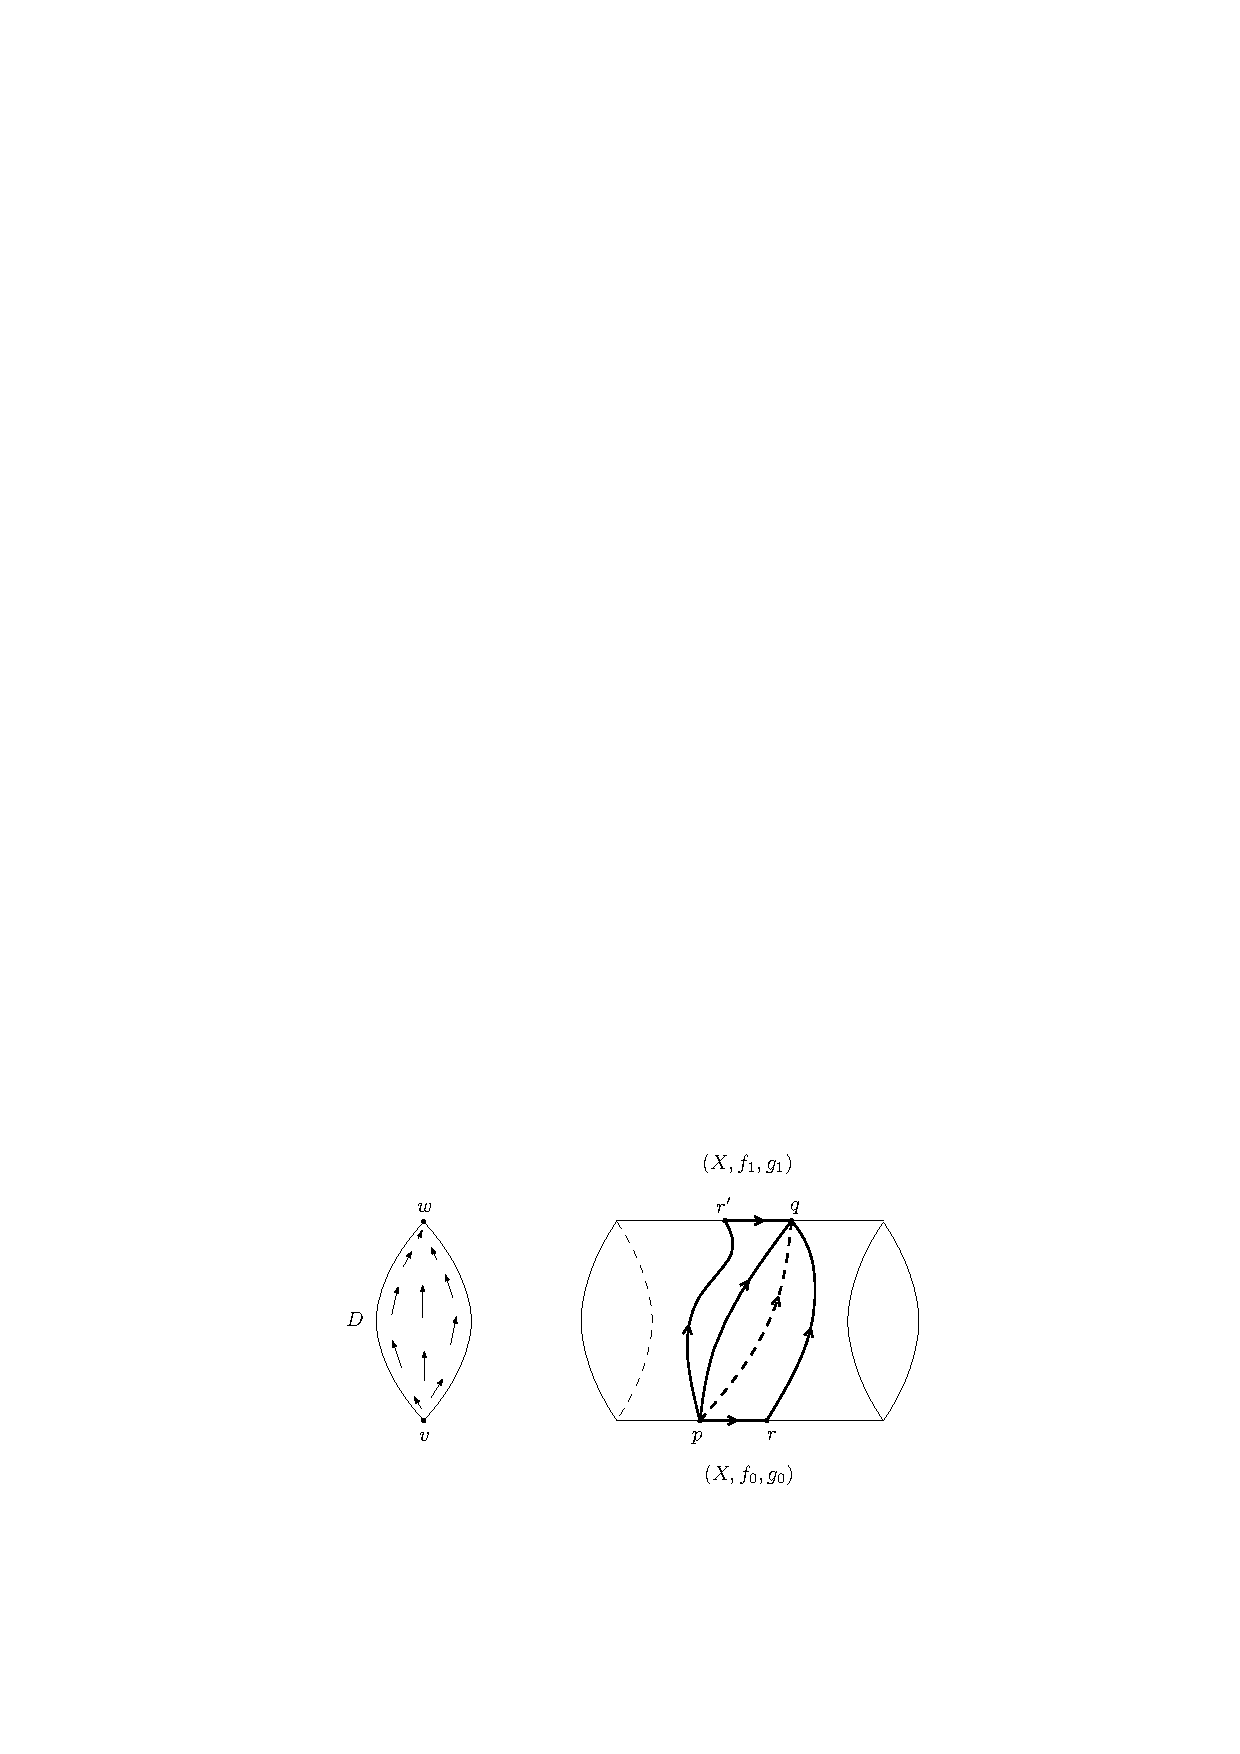
\includegraphics[scale=1]{graphics/digon}
\caption{Counting flow lines from $(v,p)$ to $(w,q)$ in $D \times X$}
\label{digon}
\end{figure}
\end{proof}


Now we have that $\Phi_{\Gamma*}$ depends only on the homotopy class of the path $\Gamma$. However, all paths between any two pairs are homotopic (since $C^\infty(M)$ and the space of metrics is contractible), so $\Phi_{\Gamma*}$ does not even depend on $\Gamma$. This means that just by virtue of the construction of Morse homology we always get a natural map $\Phi_* : HM_*(f_0,g_0) \rightarrow HM_*(f_1,g_1)$ for any Morse-Smale pairs $(f_0,g_0)$ and $(f_1,g_1)$. We want to show that this naturally defined map is an isomorphism, which means that Morse homology depends only on $X$.

In order to show this we need composition of paths $\Gamma_2 * \Gamma_1$ (where $\Gamma_1$'s ending point is $\Gamma_2$'s starting point) to correspond to composition of induced maps $\Phi_{\Gamma_2*} \circ \Phi_{\Gamma_1*}$; that is, we need to show that $\Phi_{\Gamma_2*\Gamma_1}$ is chain homotopic to $\Phi_{\Gamma_2*} \circ \Phi_{\Gamma_1*}$. To show this we need to introduce a new apparatus similar to the digon from above. First, slightly homotope $\Gamma_2 * \Gamma_1$ so that it is admissible. Then, let $T$ be a trigon; that is, a 2-manifold with 3 corners, $u,v,w$, and 3 edges, $e_{uv},e_{vw},e_{uw}$. Let $\Omega = \lcb (f_d,g_d) \st d \in T \rcb$ be a family of pairs such that $(f_u,g_u)=\Gamma_1(0)$, $(f_v,g_v)=\Gamma_1(1)=\Gamma_2(0)$, $(f_w,g_w)=\Gamma_2(1)$, and such that $\Omega$ restricted to $e_{uv}$ is $\Gamma_1$, restricted to $e_{vw}$ is $\Gamma_2$, and restricted to $e_{uw}$ is $\Gamma_2 * \Gamma_1$. Put a metric $\widetilde g$ on $T$ such that the edges are of length one, and take a smooth function $\widetilde f : T \rightarrow \mathbb R$ whose only critical points are $u,v,w$ with $\mu(u)=2,\mu(v)=1$ and $\mu(w)=0$, and the negative gradient $\widetilde V=-\nabla_{\widetilde g} \widetilde f$ is tangent to the edges of $T$ and like $(1+t)t(1-t)$. Define the vector field $V_\Omega$ on $T \times X$ by $V_\Omega = \widetilde V + V_d$, where $V_d = -\nabla_{g_d} f_d$. We can define the critical points, flow lines, ascending and descending manifolds of $V_\Omega$ in the regular way. We say that $\Omega$ is an admissible family if the ascending and descending manifolds of $V_\Omega$ intersect transversely.

The critical points of index $i$ of $V_\Omega$ are precisely
\[ \crit_i(V_\Omega) = \lcb u \rcb \times \crit_{i-2}(f_u) \cup \lcb v \rcb \times \crit_{i-1}(f_v) \cup \lcb w \rcb \times \crit_i(f_w) \]
For critical points $P,Q$ of $V_\Omega$ let $\mathcal M^\Omega(P,Q)$ be the moduli space of flow lines from $P$ to $Q$, and $\widehat{\mathcal M}^\Omega(P,Q)$ the moduli space of unparameterized flow lines. For any admissible family $\Omega$ we have that $\mathcal M^\Omega(P,Q)$ is a $(\mu(P)-\mu(Q))$-dimensional manifold and $\widehat{\mathcal M}^\Omega(P,Q)$ is a $(\mu(P)-\mu(Q)-1)$-dimensional manifold. Like the spaces $\widehat{\mathcal M}^\Psi$ considered above, the space $\widehat{\mathcal M}^\Omega(P,Q)$ may have boundary, and their compactifications can be quite complicated. The description of this space can vary greatly depending on where $P$ and $Q$ are, so we state the results we need in the only two special cases used.

If $\mu(P)=\mu(Q)+1$, then $\widehat{\mathcal M}^\Omega(P,Q)$ is already compact, and since it is a 0-dimensional manifold we have that it is just a finite set of points. If $P=(u,p)$ and $Q=(w,q)$ with $\mu(p)=i=\mu(q)$, then $\mu((u,p))=i+2$ and $\mu((w,q))=i$, hence $\widehat{\mathcal M}^\Omega((u,p),(w,q))$ is a 1-dimensional manifold and has a natural compactification to a 1-dimensional manifold $\overline{\widehat{\mathcal M}^\Omega((u,p),(w,q))}$ with boundary by adding broken flow lines. The broken flow lines that pass through one intermediate critical point of index $i+1$ are contained in the boundary, and these points are precisely
\[ \crit_{i+1}(V_\Omega) = \lcb u \rcb \times \crit_{i-1}(f_u) \cup \lcb v \rcb \times \crit_{i}(f_v) \cup \lcb w \rcb \times \crit_{i+1}(f_w) \]
But, we also have boundary points coming from those flow lines that stay in the $e_{uw} \times X$ slice for all time. These flow lines correspond to $\widehat{\mathcal M}^{\Gamma_2*\Gamma_1}((u,p),(w,q))$, hence
\begin{align*}
\partial\overline{\widehat{\mathcal M}^\Omega((u,p),(w,q))} &= \widehat{\mathcal M}^{\Gamma_2*\Gamma_1}((u,p),(w,q)) \\
  &\cup \bigcup_{r  \in \crit_{i-1}(f_u)} \widehat{\mathcal M}^\Omega((u,p),(u,r))  \times \widehat{\mathcal M}^\Omega((u,r),(w,q)) \\
  &\cup \bigcup_{r' \in \crit_{i+1}(f_w)} \widehat{\mathcal M}^\Omega((u,p),(w,r')) \times \widehat{\mathcal M}^\Omega((w,r'),(w,q)) \\
  &\cup \bigcup_{s  \in \crit_i(f_v)}     \widehat{\mathcal M}^\Omega((u,p),(v,s))  \times \widehat{\mathcal M}^\Omega((v,s),(w,q)) 
\end{align*}
Note that flow lines that stay in the $u \times X$ slice correspond to $\widehat{\mathcal M}^{f_u}(p,r)$, and similarly for flows that stay in the $w \times X$ slice. Therefore we have
\[ \widehat{\mathcal M}^\Omega((u,p),(u,r)) = \widehat{\mathcal M}^{f_u}(p,r) \]
\[ \widehat{\mathcal M}^\Omega((w,r'),(w,q)) = \widehat{\mathcal M}^{f_w}(r',q) \]
Further, the flows from $(u,p)$ to $(v,s)$ must stay in the $e_{uv} \times X$ slice and similarly for flows from $(v,s)$ to $(w,q)$, so we have
\[ \widehat{\mathcal M}^\Omega((u,p),(v,s)) = \widehat{\mathcal M}^{\Gamma_1}((u,p),(v,s)) \]
\[ \widehat{\mathcal M}^\Omega((v,s),(w,q)) = \widehat{\mathcal M}^{\Gamma_2}((v,s),(w,q)) \]
See \cref{trigon}.

We define $G_\Omega : CM_i(f_u,g_u) \rightarrow CM_{i+1}(f_w,g_w)$ on $p \in \crit_i(f_u)$ by
\[ G_\Omega(p) = \sum_{q \in \crit_{i+1}(f_w)} \# \widehat{\mathcal M}^\Omega((u,p),(w,q)) \cdot q \]
and extend linearly to all of $CM_i(f_u,g_u)$.



\begin{prop}
\label{concatenation of paths induces composition}
$\Phi_{\Gamma_2 * \Gamma_1}$ is chain homotopic to $\Phi_{\Gamma_2} \circ \Phi_{\Gamma_1}$.
\end{prop}
\begin{proof}
Let $\Omega = \lcb (f_d,g_d) \st d \in T \rcb$ be an admissible family between $\Gamma_1,\Gamma_2$ and $\Gamma_2*\Gamma_1$. We claim that the map $G_\Omega$ defined above is a chain homotopy between $\Phi_{\Gamma_2 * \Gamma_1}$ and $\Phi_{\Gamma_2} \circ \Phi_{\Gamma_1}$, i.e. if we set $E = \partial^w \circ G_\Omega + G_\Omega \circ \partial^u - \Phi_{\Gamma_2 * \Gamma_1} + \Phi_{\Gamma_2} \circ \Phi_{\Gamma_1}$, then the coefficient of $q \in \crit_i(f_w)$ in $E(p)$ is zero for all $p \in \crit_i(f_u)$.

We can easily compute
\begin{align*}
G_\Omega \circ \partial^u(p) &= \sum_{q \in \crit_i(f_w)} \sum_{r \in \crit_{i-1}(f_u)} \# \widehat{\mathcal M}^{f_u}(p,r) \cdot \#\widehat{\mathcal M}^\Omega((u,r),(w,q)) \cdot q \\
\partial^w \circ G_\Omega(p) &= \sum_{q \in \crit_i(f_w)} \sum_{r' \in \crit_{i+1}(f_w)} \# \widehat{\mathcal M}^\Omega((u,p),(w,r')) \cdot \# \widehat{\mathcal M}^{f_w}(r',q) \cdot q \\
\Phi_{\Gamma_2} \circ \Phi_{\Gamma_1}(p) &= \sum_{q \in \crit_i(f_w)} \sum_{s \in \crit_i(f_v)} \# \widehat{\mathcal M}^{\Gamma_1}((u,p),(v,r)) \cdot \# \widehat{\mathcal M}^{\Gamma_2}((v,r),(w,q)) \cdot q 
\end{align*}
Now it is clear that the coefficient of $q \in \crit_i(f_w)$ in $E(p)$, where $p \in \crit_i(f_u)$, is precisely $\# \partial \overline{\widehat{\mathcal M}^\Omega((u,p),(w,q))}$, hence zero.

\begin{figure}[tb]
\centering
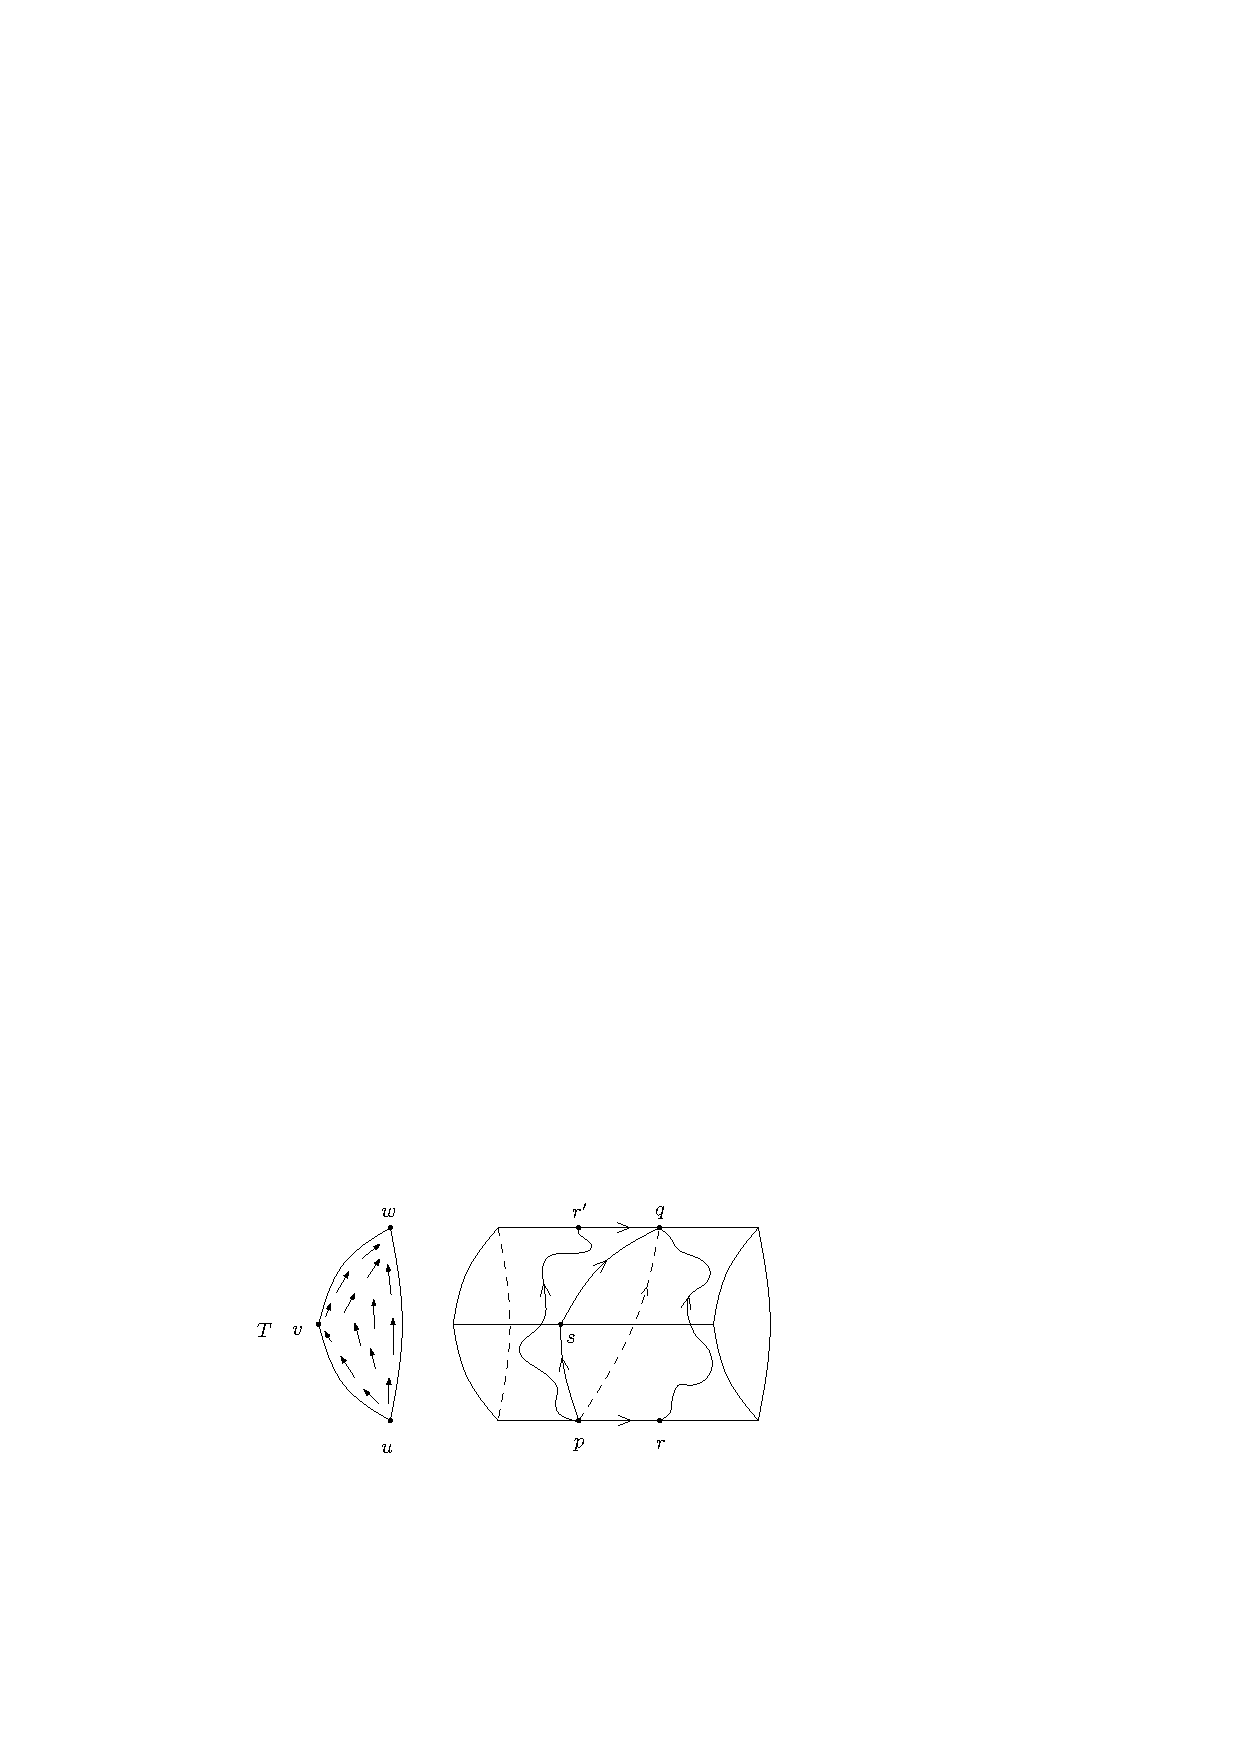
\includegraphics[scale=1]{graphics/trigon}
\caption{Counting flow lines from $(u,p)$ to $(w,q)$ in $T \times X$}
\label{trigon}
\end{figure}
\end{proof}



Combining \cref{constant path induces identity,induced maps of homotopic paths are homotopic,concatenation of paths induces composition} we get invariance of Morse homology.
\begin{cor}
For any two Morse-Smale pairs $(f_0,g_0)$ and $(f_1,g_1)$, the Morse homologies $HM_*(f_0,g_0)$ and $HM_*(f_1,g_1)$ are naturally isomorphic.
\end{cor}



\subsection{Orientations on Moduli Spaces}
\label{Geometric Orientations and Orientations on Moduli Spaces}


There are (at least) two ways to introduce orientations on our moduli spaces $\mathcal M^f(p,q)$ and $\widehat{\mathcal M}^f(p,q)$ so that we can define the Morse complex with $\mathbb Z$ coefficients. One way is geometric and technically the simplest way to define orientations, but it does not generalize to the infinite dimensional versions of Morse homology. The other way is very technical and uses high powered machinery from functional analysis, but also has obvious interpretations in the infinite dimensional setting. We will give a superficial description of both of these orientations, and explain why they should give the same end result.

For the geometric orientations we must assume that our Riemannian manifold $(X^n,g)$ is oriented. Let us also fix a Morse function $f$ on $X$ so that $(f,g)$ is a Morse-Smale pair. We stated in \cref{ascending and descending manifolds are manifolds} that the ascending manifold $\mathscr A(p)$ and descending manifold $\mathscr D(p)$ of a critical point $p \in \crit_i(f)$ are smoothly embedded discs of dimension $i$ and $n-i$, respectively. Let us define $\mathscr M^f(p,q)$ to be the intersection $\mathscr D(p) \cap \mathscr A(q)$, which is a submanifold of dimension $\mu(p)-\mu(q)$. We get an $\mathbb R$ action on $\mathscr M^f(p,q)$ via the 1-paremeter group of diffeomorphisms $\varphi_t : X \rightarrow X$ generated by $-\nabla_g f$: for $t \in \mathbb R$ and $x \in \mathscr M^f(p,q)$ we define $t \cdot x = \varphi_t(x)$. This action is free and smooth, so $\widehat{\mathscr M}^f(p,q) = \mathscr M^f(p,q)/\mathbb R$ is a $(\mu(p)-\mu(q)-1)$-dimensional manifold.
\begin{prop}
\label{geometric and analytic moduli spaces}
The map $\phi : \mathcal M^f(p,q) \rightarrow \mathscr M^f(p,q)$ defined by $\phi(u)=u(0)$ is a diffeomorphism, and for each $t \in \mathbb R$ the following diagram commutes
\[
\xymatrix
{
	\mathcal M^f(p,q) \ar[r]^{t \cdot} \ar[d]_\phi & \mathcal M^f(p,q) \ar[d]^\phi \\
	\mathscr M^f(p,q) \ar[r]_{t \cdot} & \mathscr M^f(p,q)
}
\]
where $t \cdot$ on the horizontal arrows denotes the $\mathbb R$ action on the respective spaces. In particular, $\widehat{\mathscr M}^f(p,q)$ is diffeomorphic to $\widehat{\mathcal M}^f(p,q)$.
\end{prop}

Let us put an arbitrary orientation on $T_p \mathscr D(p)$ for all $p \in \crit(f)$. Since $T_p \mathscr D(p) \oplus T_p \mathscr A(p) = T_p X$, and $T_p X$ is oriented by assumption, we get an induced orientation on $T_p \mathscr A(p)$. These orientations at $p$ uniquely extend to coherent orientations on all of $\mathscr A(p)$ and $\mathscr D(p)$, and so now all ascending and descending submanifolds are oriented. Now the spaces $\mathscr M^f(p,q)$ get an induced orientation, as described in \cref{Transversality and Intersection Theory}, so we can orient $\mathcal M^f(p,q)$ by requiring the isomorphism $\phi$ in \cref{geometric and analytic moduli spaces} to be orientation preserving.


\unfinished



\comment{
Assume now that $p \in \crit_i(f)$ and $q \in \crit_{i-1}(f)$ so that $\widehat{\mathcal M}^f(p,q)$ is a compact, 0-dimensional manifold (i.e. a finite collection of points). Using the orientations on the descending and ascending manifolds defined above we will show how to assign orientation signs to this discrete set of unparameterized flow lines.

A point $\widehat{u}$ in $\widehat{\mathcal M}^f(p,q)$ is an unparameterized flow line from $p$ to $q$, so let $u$ be any lift of $\widehat{u}$ and $x$ any point in the image of $u$. The vector $-\nabla_g f(x)$ in $T_x \mathscr D(p)$ can be completed to a positive basis $(-\nabla_g f(x),\sigma_x)$ for $T_x \mathscr D(p)$ (in the degenerate case that $\dim T_x \mathscr D(p)=1$ we just take $\sigma_x$ to be a positive basis for the tangent space). Then, if we let $\overline{\sigma}_x$ be a positive basis for $T_x \mathscr A(q)$ we get a basis $(\sigma_x,\overline\sigma_x)$ for $T_x X$ (note that $\sigma_x$ has $i-1$ basis vectors and $\overline{\sigma}_x$ has $n-(i-1)$ basis vectors, so the dimensions do add up correctly). We define the sign of $\widehat{u}$ to be  $n(\widehat{u})=+1$ if $(\sigma_x,\overline{\sigma}_x)$ is a positive basis for $T_x X$, and $n(\widehat{u})=-1$ if it is a negative basis. Finally, we define
\[ n(p,q) = \sum_{\widehat{u} \in \widehat{\mathcal M}^f(p,q)} n(\widehat{u}) \]
Now we can define the Morse complex with integer coefficients. Let $CM_i(f,g)$ be the free abelian group generated by the critical points of index $i$, and define the map $\partial : CM_i(f,g) \rightarrow CM_{i-1}(f,g)$ on $p \in \crit_i(f)$ by
\[ \partial(p) = \sum_{q \in \crit_{i-1}(f)} n(p,q) \cdot q \]
One can show that $\partial \circ \partial = 0$, so we define the Morse homology of the pair $(f,g)$ to be $HM_*(f,g) = H_*(CM_*(f,g),\partial)$. In order for this definition to be well-defined we need to make sure that $HM_*(f,g)$ is independent of our choices made in defining $n(p,q)$, or in particular, the definition of $n(\widehat{u})$. It is clear that the value of $n(\widehat{u})$ does not depend on the lift $u$ of $\widehat{u}$ since any time lifts differ by a linear translation, nor does it depend on the point $x$ in the range of $u$ since the tangent bundle of $\mathscr D(p)$ is trivial. The last choices made in defining $n(\widehat u)$ were in $\sigma_x$ and $\overline\sigma_x$ by requiring that $(-\nabla_g f(x),\sigma_x)$ and $(\sigma_x,\overline\sigma_x)$ be positive, for we could have required instead that $(\sigma_x,-\nabla_g f(x))$ and/or $(\overline\sigma_x,\sigma_x)$ be positive. However, if $\partial$ is the boundary operator computed with respect to one of these choices and $\partial'$ is the boundary computed with respect to another set of choices, we clearly have $\partial = \pm \partial'$. Therefore the kernels and images of $\partial$ and $\partial'$ are equal, hence the homology computed with respect to these maps are isomorphic.

This homology theory is also independent of the Morse-Smale pair $(f,g)$ used to define it (the proof is similar to our proof for $\mathbb Z/2$ coefficients, in spirit, but orientations make it more difficult). More generally, we can define the Morse homology of $(f,g)$ with coefficients in any abelian group $A$ by defining $HM_*(f,g;A) = H(CM_*(f,g) \otimes A,\partial \otimes \id_A)$. Again this does not depend on the pair $(f,g)$, so we can also write this as $HM_*(X;A)$.
}









\subsection{Applications}
\label{Morse Homology Applications}

The Morse inequalities are set of nice results that put topological restrictions on a space according to what type of Morse functions the space admits, and they nearly come for free with the definition of Morse homology. It was these inequalities that inspired Floer to define his infinite dimensional generalization of Morse homology in order to prove the Arnold conjecture. Since $HM_*(f,g)$ is isomorphic to $H_*(X)$ we already have that the Euler characteristic of $X$ can be computed by $\chi(X) = \sum (-1)^i \# \crit_i(f)$ for any Morse function $f$ on $X$. The Morse inequalities strengthen this quite a bit.

First we need to prove a general result concerning finitely generated chain complexes.
\begin{thm}[Euler-Poincar\'{e} Theorem]
Take any finitely generated chain complex
\[ 0 \longrightarrow C_n \stackrel{\partial_n}{\longrightarrow} C_{n-1} \stackrel{\partial_{n-1}}{\longrightarrow} \cdots \stackrel{\partial_2}{\longrightarrow} C_1 \stackrel{\partial_1}{\longrightarrow} C_0 \longrightarrow 0 \]
and let $H_i = H_i(C_*,\partial_*)$. Then
\[ \sum_{i=0}^n (-1)^i \rank C_i = \sum_{i=0}^n (-1)^i \rank H_i \]
\end{thm}
\begin{proof}
At each $i=0,\ldots,n$ we have a short exact sequence
\[ 0 \longrightarrow \ker \partial_i \longrightarrow C_i \stackrel{\partial_i}{\longrightarrow} \image \partial_i \longrightarrow 0 \]
hence $\rank C_i = \rank \ker \partial_i + \rank \image \partial_i$. We also have a short exact sequence
\[ 0 \longrightarrow \image \partial_{i+1} \longrightarrow \ker \partial_i \longrightarrow H_i \longrightarrow 0 \]
hence $\rank \ker \partial_i = \rank \image \partial_{i+1} + \rank H_i$. There is a common $\rank \ker \partial_i$ in each of the equations we derived from these short exact sequences, and solving for it gives
\[ \rank \ker \partial_i = \rank C_i - \rank \image \partial_i = \rank \image \partial_{i+1} + \rank H_i \]
Therefore
\[ \sum_{i=0}^n (-1)^i \left( \rank C_i - \rank \image \partial_i \right) = \sum_{i=0}^n (-1)^i \left( \rank \image \partial_{i+1} + \rank H_i \right) \]
On the left side we have that $\rank \image \partial_i$ appears with sign $(-1)^{i+1}$, and on the right $\rank \image \partial_i$ appears with sign $(-1)^{i-1}$, hence they cancel and we are left with
\[ \sum_{i=0}^n (-1)^i \rank C_i = \sum_{i=0}^n (-1)^i \rank H_i \]
\end{proof}

\begin{thm}[Morse Inequalities]
\label{Morse inequalities}
Let $f : X^n \rightarrow \mathbb R$ be a Morse function. Let $c_i = \# \crit_i(f)$ be the number of critical points of index $i$, and let $b_i = \rank H_i(X)$ be the $i$-th Betti number of $X$. Then
\begin{equation}
\label{Morse inequality}
c_k - c_{k-1} + \cdots + (-1)^k c_0 \geq b_k - b_{k-1} + \cdots + (-1)^k b_0
\end{equation}
for all $0 \leq k \leq n$.
\end{thm}
\begin{proof}
We have $\rank HM_i(f,g) = \rank H_i(X) = b_i$ and $\rank CM_i(f,g) = \# \crit_i(f)$. Since $HM_i(f,g)$ is a subquotient of $CM_i(f,g)$, we clearly have $c_i \geq b_i$.  Let $0 \leq k \leq n$, and let $(C_*,\partial_*)$ denote the chain complex $(CM_*,\partial_*)$ truncated at $k$:
\[ 0 \longrightarrow C_k \stackrel{\partial}{\longrightarrow} C_{k-1} \stackrel{\partial}{\longrightarrow} \cdots \stackrel{\partial}{\longrightarrow} C_1 \stackrel{\partial}{\longrightarrow} C_0 \longrightarrow 0 \]
The chain complex $(C_*,\partial_*)$ is finitely generated, so by the Euler-Poincar\'{e} theorem we have
\begin{equation}
\label{Euler-Poincare applied to truncated complex}
\sum_{i=0}^k (-1)^{i+k} \rank C_i = \sum_{i=0}^k (-1)^{i+k} \rank H_i(C_*,\partial_*)
\end{equation}
The inserted signs $(-1)^k$ are necessary so that the last term $(i=k)$ in the sums are non-negative. The homology of the chain complex $(C_*,\partial_*)$ is equal to the homology of $(CF_*,\partial_*)$ in all gradings except possibly the last, so we have $\rank H_i(C_*,\partial_*)=b_i$ for all $0 \leq i \leq k-1$. For the last term we have $H_k(C_*,\partial_*)=\ker \partial_k$, hence $H_k(CM_*,\partial_*)$ is a quotient of $H_k(C_*,\partial_*)$, and so we have $b_k \leq \rank H_k(C_*,\partial_*)$. By replacing the last term $\rank H_k(C_*,\partial_*)$ in \eqref{Euler-Poincare applied to truncated complex} with the smaller term $b_k$ we obtain the Morse inequality
\[ c_k - c_{k-1} + \cdots + (-1)^k c_0 \geq b_k - b_{k-1} + \cdots + (-1)^k b_0 \]
\end{proof}






\comment{
Morse homology also gives a nice proof of Poincar\'{e} duality. In order to state this we need develop Morse cohomology. Let $CM^i(f,g) = \Hom(CM_i(f,g),\mathbb Z)$ be the dual cochain complex of $CM_*(f,g)$, and let $\delta : CM^i(f,g) \rightarrow CM^{i+1}(f,g)$ be the dual coboundary operator uniquely determined by
\[ (\delta\alpha)(x) = \alpha(\partial x) \]
for all $\alpha \in CM^i(f,g)$ and $x \in CM_{i+1}(f,g)x$. For each $p\in\crit_i(f)$, let $\alpha_p \in CM^i(f,g)$ be the cochain that acts on $q \in \crit_i(f)$ by $\alpha_p(q)=\delta_p^q$. The $\alpha_p$'s form a basis for $CM^i(f,g)$, and the map $p \mapsto \alpha_p$ provides an identification $CM_i(f,g) \cong CM^i(f,g)$. \unfinished



-----------------

get an identification $CM_i(f,g) \cong CM^i(f,g)$ by sending $p \in \crit_i(f)$ to the $i$-cochain $\alpha_p$ defined by $\alpha_p(q)=\delta_p^q$. Using this identification we can explicitly write the coboundary operator as
\[ \delta p = \sum_{q \in \crit_{i+1}(f)} \< \partial q,p \> \cdot q \]
for $p \in \crit_i(f)$. We can now define the Morse cohomology of the pair $(f,g)$ to be $HM^*(f,g)=H^*(CM^*(f,g),\delta)$, and we can define Morse cohomology with coefficients in an abelian group $A$, $H^i(f,g;A)$, by dualizing with $A$: $CM^i(f,g;A)=\Hom(CM_i(f,g),A)$. Morse homology and cohomology are related by the (un-naturally) splitting, short exact sequence of the universal coefficient theorem:
\[ HM^i(f,g;A) \cong \Ext(HM_{i-1}(f,g),A) \oplus \Hom(HM_i(f,g),A) \]
Since $HM_*(f,g)$ does not depend on $(f,g)$ we also have that $HM^*(f,g;A)$ does not depend on $(f,g)$. Further, since $HM_*(f,g) \cong H_*(X)$, we also have $HM^*(f,g) \cong H^*(X)$.

\begin{thm}[Poincar\'{e} Duality]
For a closed, orientable manifold $X^n$, there is a natural isomorphism $PD : H_i(X) \rightarrow H^{n-i}(X)$.
\end{thm}
\begin{proof}
We will only prove this with $\mathbb Z/2$ coefficients, so we do not even need $X$ to necessarily be orientable. Let $(f,g)$ be a Morse-Smale pair on $X$, then $(-f,g)$ is also a Morse-Smale pair on $X$ with the property $\crit_i(-f)=\crit_{n-i}(f)$. Therefore we get a naturally induced isomorphism 
\[ \Phi : HM_*(f,g) \stackrel{\cong}{\rightarrow} HM_*(-f,g) \]
Let $\varphi : CM_i(-f) \rightarrow CM^{n-i}(f)$ be the isomorphism defined by $\varphi(p) = \< p, - \>$, where on the left we think of $p \in \crit_i(-f)$ and on the right we think of $p \in \crit_{n-i}(f)$.
\end{proof}
}






\subsection{Witten's Complex}
\label{Witten's Complex}


In a paper on supersymmetry in physics, Witten was able to rediscover the Morse inequalities (see \cref{Morse inequalities}) and Morse (co)homology by considering a simple supersymmetric theory on the exterior bundle $\Lambda^* T^* X$ of a compact, orientable manifold $X^n$. First we discuss the mathematical content of his results without mentioning any of the physics.

Let us recall some of the basic results of Hodge theory. If we put a metric $g$ on $X$, then we get an induced volume form $\vol_g$, and we get a star operator $\star : \Omega^k(X) \rightarrow \Omega^{n-k}(X)$ which satisfies $\star^2 = (-1)^{k(n-k)} \id_{\Omega^k(X)}$. The de Rham operator $d : \Omega^k(X) \rightarrow \Omega^{k+1}(X)$ has a formal adjoint $\delta : \Omega^k(X) \rightarrow \Omega^{k-1}(X)$, which can be defined by $\delta = (-1)^{kn+n+1} \star d \star$. We define the Laplace operator $\Delta : \Omega^k(X) \rightarrow \Omega^k(X)$ by $\Delta = d\delta+\delta d$. This operator has discrete spectrum, and decomposes $\Omega^k(X)$ into eigenspaces
\[ \Omega^k(X) = \bigoplus_{\lambda \in \mathbb R} E_\lambda^k \ \ \ \ \ \text{where} \ \ \ \ \ E_\lambda^k = \lcb \omega \in \Omega^k(X) \st \Delta \omega = \lambda \omega \rcb \]
The fundamental theorem of Hodge theory is the following.
\begin{thm}[Hodge's Theorem]
$E_0^k \cong H_{dR}^k(X)$
\end{thm}

So, we can think of $(E_0^*,d)$ has a finite dimensional chain complex (the differential happens to be zero) that ``computes'' the homology of the infinite dimensional chain complex $(\Omega^*(X),d)$. We clearly have $d(E_\lambda^k) \subseteq E_\lambda^{k+1}$, so for $\lambda > 0$ we also get a chain complex
\[ 0 \longrightarrow E_\lambda^0 \stackrel{d}{\longrightarrow} E_\lambda^1 \stackrel{d}{\longrightarrow} \cdots \stackrel{d}{\longrightarrow} E_\lambda^n \longrightarrow 0 \]
However, this sequence is exact. To see this, let $\omega \in E_\lambda^k$ such that $d\omega=0$, then
\[ d\left( \lambda^{-1} \delta \omega \right) = \lambda^{-1} d\delta \omega = \lambda^{-1} \Delta \omega = \lambda^{-1} \lambda \omega = \omega \]
therefore $\omega$ is exact. This means that the homology of the complex $(E_\lambda^*,d)$ is zero. Now, for fixed $\lambda_0 > 0$, let 
\[ \Omega_{\lambda_0}^k = \bigoplus_{\lambda \leq \lambda_0} E_\lambda^k \]
That is, $\Omega_{\lambda_0}^*$ consists of all the eigenforms of $\Delta$ with eigenvalue less than or equal to $\lambda_0$. Now, the restriction of $d$ to $\Omega_{\lambda_0}^*$ gives a \emph{finite} dimensional complex $(\Omega_{\lambda_0}^*,d)$, and since this complex is a direct sum of exact sequences (when $\lambda \in (0,\lambda_0]$) and a sequence with homology equal to de Rham homology (when $\lambda=\lambda_0$), we have
\[ H^*( \Omega_{\lambda_0}^*,d ) = H_{dR}^*(X) \]
If we have chosen $\lambda_0$ large enough so that there is an eigenvalue of $\Delta$ in $(0,\lambda_0]$, then we have replaced the \emph{infinite} dimension complex $(\Omega^*,d)$ with a non-trivial \emph{finite} dimensional complex $(\Omega_{\lambda_0}^*,d)$ without changing the homology.

We now repeat these same ideas with a slight variation of Hodge theory. For a fixed Morse function $f : X \rightarrow \mathbb R$ and real parameter $t$ we define the operator $d_t : \Omega^k(X) \rightarrow \Omega^{k+1}(X)$ by
\[ d_t = e^{-ft} d e^{ft} \]
that is, we conjugate the de Rham operator by the linear isomorphism $\omega \mapsto e^{-ft} \omega$. The function $f$ will remained fixed in our discussion, but we will be taking $t$ to be large soon, so we only put $t$ in our notation. We clearly have $d_t^2 = 0$, and this operator has the formal adjoint $\delta_t : \Omega^k(X) \rightarrow \Omega^{k-1}(X)$ defined by
\[ \delta_t = e^{ft} \delta e^{-ft} \]
and so we define the Laplacian $\Delta_t = d_t\delta_t + \delta_t d_t$. We can also define the homology groups $H_t^*(X) = \ker d_t / \image d_t$, but the isomorphism $\Omega^k \rightarrow \Omega^k$ given by $\omega \mapsto e^{-ft} \omega$ descends to an isomorphism $H_{dR}^*(X) \cong H_t^*(X)$, so this homology theory does not give us anything new. Like before we get an eigenspace decomposition
\[ \Omega^k(X) = \bigoplus_{\lambda \in \mathbb R} E_\lambda^k(t) \ \ \ \ \ \text{where} \ \ \ \ \ E_\lambda^k(t) = \lcb \omega \in \Omega^k(X) \st \Delta_t \omega = \lambda \omega \rcb \]
We also have a Hodge-like theorem that says $E_0^k(t) \cong H_{dR}^k(X)$. Also like before, for $\lambda > 0$ we have an exact sequence
\[ 0 \longrightarrow E_\lambda^0(t) \stackrel{d_t}{\longrightarrow} E_\lambda^1(t) \stackrel{d_t}{\longrightarrow} \cdots \stackrel{d_t}{\longrightarrow} E_\lambda^n(t) \longrightarrow 0 \]
So, if for fixed $\lambda_0 > 0$ we define $\Omega_{\lambda_0}^k(t) = \bigoplus_{\lambda \leq \lambda_0} E_\lambda^k(t)$, then the \emph{finite} dimensional complex $(\Omega_{\lambda_0}^*(t),d_t)$ has the same homology as $(\Omega^*,d)$. At this point Witten claims that for sufficiently large $t >> 0$, the dimensions $\dim \Omega_{\lambda_0}^k(t)$ become independent of $t$, and so let us write $(\Omega_{\lambda_0}^*(\infty),d_\infty)$ to denote this ``stabilized'' chain complex. In fact, Witten shows that
\[ \dim \Omega_{\lambda_0}^k(\infty) = \# \crit_k(f) = c_k \]
As we saw in \cref{Morse inequalities}, whenever we have a finite dimensional complex whose chain groups correspond to critical points of a Morse function, and whose homology computes the homology of $X$, then we get the Morse inequalities for free. So, we have proved the Morse inequalities by considering a variation of Hodge theory.

Now let us see the physical ideas behind the above results. Using the definition of $d_t$ and $\delta_t$, one can easily compute that these operators act on a $k$-form $\omega \in \Omega^k(X)$ by
\[ d_t \omega = d\omega + t df \wedge \omega \ \ \ \ \ \ \ \delta_t \omega = \delta \omega - t i_{df} \omega \]
If we choose coordinates $(x,U)$ on $X$, and define the operators $A_i^* \omega = i_{\pfrac{}{x^i}} \omega$ and $A_i \omega = dx^i \wedge \omega$, then one can show that $\Delta_t$ can be written as
\[ \Delta_t = \Delta + t^2 \norm{df}^2 + t \sum_{i=1}^n \frac{\partial^2 f}{\partial x^i \partial x^j} [A_i^*, A_j] \]
As $t$ gets large we expect the eigenforms of this operator to be increasingly concentrated at the critical points of $f$. This leads us to look around the critical points. If $p \in \crit(f)$, then we can choose normal coordinates $(x,U)$ around $p$ such that $f$ is of the form
\[ f = f(p) + \sum_{i=1}^n \lambda_i (x^i)^2 + O(x^3) \]
where the $\lambda_i$'s are the eigenvalues of the Hessian of $f$ at $p$. In these coordinates, if we ignore terms of order 3 and above, then Laplacian $\Delta_t$ can be approximated by
\[ \widetilde{\Delta}_t = \sum_{i=1}^n \left( - \frac{\partial^2}{(\partial x^i)^2} + t^2 \lambda_i^2 (x^i)^2 + t \lambda_i [A_i^*,A_i] \right) \]
This looks like a simple harmonic oscillator, plus some other operator. Recall that for $a>0$, the simple harmonic oscillator
\[ H = -\frac{d^2}{dx^2} + a^2 x^2 \]
has spectrum $\lcb (2k+1)a \st k=0,1,\ldots \rcb$. So, let us write our approximation of the Laplacian as
\[ \widetilde{\Delta}_t = \sum_{i=1}^n \left( H_i + t\lambda_i K_i \right) \]
where $H_i = -\partial^2 / (\partial x^i)^2 + t^2\lambda_i (x^i)^2$ and $K_i = [A_i^*,A_i]$. The $H_i$'s commute with themselves, the $K_i$'s commute with themselves, and the $H_i$'s commute with the $K_j$'s. Therefore the spectrum of $\widetilde\Delta_t$ is the sum of the spectrum of the $H_i$'s and $K_i$'s. The spectral of $H_i$ is given by $\lcb (2N_i+1)t|\lambda_i| \st N_i=0,1,\ldots \rcb$. One can easily compute that
\[ K_i dx^{i_1} \wedge \cdots \wedge dx^{i_k} = \begin{cases} +dx^{i_1} \wedge \cdots \wedge dx^{i_k} & i \in \lcb i_1,\ldots,i_k \rcb \\ -dx^{i_1} \wedge \cdots \wedge dx^{i_k} & i \notin \lcb i_1,\ldots,i_k \rcb \end{cases} \]
so the eigenvalues of this operator are just $+1$'s and $-1$'s. In fact, the number of $+1$ eigenvalues is precisely $k$. Now, the spectrum of $\widetilde\Delta_t$ can be written as the set
\[ \lcb t \sum_{i=1}^n \left( (2N_i+1)|\lambda_i| + n_i \lambda_i \right) : \substack{\displaystyle N_i=0,1,\ldots \\ \displaystyle n_i = \pm 1 \\ \displaystyle \# \lcb n_i=+1 \rcb = k} \rcb \]
What choice of $N_i$ and $n_i$ give zero? If we rewrite the summand as $2N_i|\lambda_i| + |\lambda_i n_i| + n_i \lambda_i$, then we see that we are forced to have $N_i=0$ and $n_i = -\sign(\lambda_i)$. Therefore, there is exactly one zero eigenvalue of $\widetilde\Delta_t$, and all other eigenvalues blow up to $\infty$ since they are proportional to $t$. Further, associated eigenform is a $k$-form, where
\[ k = \# \lcb n_i = +1 \rcb = \# \lcb \lambda_i < 0 \rcb = \mu(p) \]
So, at each critical point $p \in \crit(f)$, we are able to associate a $\mu(p)$-form $\omega$ such that $\widetilde\Delta_t \omega = 0$. Since $\widetilde\Delta_t$ is only an approximation of $\Delta_t$, we do not necessarily have that $\Delta_t \omega = 0$. Therefore, the number of $k$-forms $\omega$ which satisfy $\widetilde\Delta_t \omega = 0$ at some critical point of index $k$ (i.e. the number of critical points of index $k$) is greater than or equal to the number of $k$-forms with $\Delta\omega = 0$ (i.e. the $k$-th Betti number of $X$). This proves the weak Morse inequalities.













\newpage
\section{Heegaard Floer Homology}
\label{Heegaard Floer Homology}


\subsection{Construction for 3-Manifolds}
\label{Construction for 3-Manifolds}


The Morse homology discussed in the previous section has inspired variations that usually go under the heading of Floer-type theories. These theories start with some differential equation (in Morse homology this was the negative gradient flow equation), then one forms a graded group freely generated by some points in a space or some other objects, and then one defines a differential to count the number of solutions to the differential equation that start at one point and end at another. Hopefully the differential squares to zero so that one can define the homology groups, and hopefully the homology groups do not depend on the various choices used in the construction of this homology theory. We now follow this plan to build a homology theory for 3-manifolds from Heegaard diagrams.

\subsubsection*{General Idea}

First, we will give a general idea of the object we are trying to construct. The details in this construction are very difficult, like it was for Morse homology, requiring a lot of machinery from analysis and symplectic geometry. Let $(\Sigma,\alpha_1,\ldots,\alpha_g,\beta_1,\ldots,\beta_g)$ be a genus $g$ Heegaard diagram for a 3-manifold $Y$, and assume the $\balpha$ and $\bbeta$ curves are in general position so that they intersect transversally. Let us also fix a base point $z$ in the complement of the $\balpha$ and $\bbeta$ curves. We can form the \textbf{symmetric product} $\Sym^g(\Sigma)$ of $\Sigma$, defined to be the quotient of $\Sigma^{\times g}$ under the action of $S_g$ permuting the components of $\Sigma^{\times g}$, i.e. $\Sym^g(\Sigma)$ consists of $g$-tuples of unordered points of $\Sigma$. Even though $S_g$ does not act freely on $\Sigma$, we do have that $\Sym^g(\Sigma)$ is a smooth manifold, and in fact a complex structure $\mathfrak j$ on $\Sigma$ induces a complex structure $\Sym^g(\mathfrak j)$ on $\Sym^g(\Sigma)$. 

Since the $\balpha$ curves never intersect each other (and similarly for the $\bbeta$ curves), we have that the products
\[ \mathbb T_\alpha = \alpha_1 \times \cdots \times \alpha_g \ \ \ \ \ \ \mathbb T_\beta = \beta_1 \times \cdots \times \beta_g \]
are smoothly embedded submanifolds of $\Sym^g(\Sigma)$, and $\mathbb T_\alpha \pitchfork \mathbb T_\beta$, hence the intersect consists of finitely many points. The base point $z$ determines a codimension 2 submanifold $V_z$ of $\Sym^g(\Sigma)$ defined by
\[ V_z = \lcb z \rcb \times \Sym^{g-1}(\Sigma) \subset \Sym^g(\Sigma) \]
Clearly $V_z$ is disjoint from the tori $\mathbb T_\alpha$ and $\mathbb T_\beta$. 

Let $\mathbb D \subset \mathbb C$ denote the unit disc, and let $e_1 = \partial\mathbb D \cap \lcb \re(z) \geq 0 \rcb$ and $e_2 = \partial\mathbb D \cap \lcb \re(z) \leq 0 \rcb$. For two intersection points $\bx,\by \in \mathbb T_\alpha \cap \mathbb T_\beta$ (this means that $\bx$ and $\by$ are unordered $g$-tuples of intersection points of the $\balpha$ and $\bbeta$ curves) we define a \textbf{Whitney disc} connecting $\bx$ to $\by$ to be a continuous map $u : \mathbb D \rightarrow \Sym^g(\Sigma)$ such that $u(-i)=\bx$, $u(i)=\by$, $u(e_1) \subset \mathbb T_\alpha$ and $u(e_2) \subset \mathbb T_\beta$. Let $\pi_2(\bx,\by)$ denote the homotopy classes of Whitney discs from $\bx$ to $\by$.

We define a function $n_z : \pi_2(\bx,\by) \rightarrow \mathbb Z$ to be the algebraic intersection number of a disc $\phi : \mathbb D \rightarrow \Sym^g(\Sigma)$ with the submanifold $V_z$. For a Whitney disc $\phi$, let $\mathcal M(\phi)$ denote the moduli space of pseudoholomorphic representatives of $\phi$, i.e. the set of representatives $u : \mathbb D \rightarrow \Sym^g(\Sigma)$ of $\phi$ that satisfies the Cauchy-Riemann equation
\[ \pfrac{u}{s} + i \pfrac{u}{t} = 0 \]
If we introduce the proper perturbations of our set up, then $\mathcal M(\phi)$ will be a smooth manifold, and we denote its dimension by $\mu(\phi)$. There is a natural free $\mathbb R$ acts on this space, and so we denote the quotient by $\widehat{\mathcal M}(\phi) = \mathcal M(\phi) / \mathbb R$.

With these definitions we can give an intuitive (but slightly incorrect) definition of Heegaard Floer homology. Let $\widehat{CF}(\balpha,\bbeta)$ be the Abelian group freely generated by the points in $\mathbb T_\alpha \cap \mathbb T_\beta$. We define a differential $\widehat{\partial} : \widehat{CF}(\balpha,\bbeta) \rightarrow \widehat{CF}(\balpha,\bbeta)$ on $\bx \in \mathbb T_\alpha \cap \mathbb T_\beta$ by
\[ \widehat{\partial}\bx = \sum_{\lcb \left. \substack{\by \in \mathbb T_\alpha \cap \mathbb T_\beta \\ \phi \in \pi_2(\bx,\by)} \right| \substack{n_z(\phi)=0 \\ \mu(\phi)=1} \rcb} \# \widehat{\mathcal M}(\phi) \cdot \by \]
That is, we are counting the number of pseudoholomorphic discs between two points in $\Sym^g(\Sigma)$. One can show that $\widehat\partial^2 = 0$, so we can define the homology groups $\widehat{HF}(\balpha,\bbeta)$. One can also show that $\widehat{HF}(\balpha,\bbeta)$ does not depend on the Heegaard diagram or complex structures chosen in order to define it, hence $\widehat{HF}(\balpha,\bbeta)$ is a topological invariant. Now we work to properly define these homology groups. 

\subsubsection*{Morse Functions and Pointed Heegaard Diagrams}

Let us fix a Heegaard diagram $(\Sigma,\alpha_1,\ldots,\alpha_g,\beta_1,\ldots,\beta_g)$ for our 3-manifold $Y$, where $\Sigma$ is a surface of genus $g$. Recall that this means we attach a 2-handle for each $\balpha$ and $\bbeta$ curve, the result being a 3-manifold with boundary two disjoint 2-spheres, and so we attach two 3-handles in the only way possible. So, the $\balpha$ and $\bbeta$ curves determine handlebodies $U_0$ and $U_1$ of genus $g$ such that $U_0 \cap U_1 = \Sigma$. We also have the following Morse theoretic picture of this set up. Let $f : Y \rightarrow [0,3]$ be a self-indexing Morse function with $g$ critical points of index 1, denote them by $P_1,\ldots,P_g$, and hence $g$ critical points of index 2, denote them by $Q_1,\ldots,Q_g$. Then $U_0 = f^{-1}[0,3/2], U_1=f^{-1}[3/2,3]$ and $\Sigma=f^{-1}(3/2)$, and the attaching circles can be defined by $\alpha_i = \mathscr A(P_i) \cap \Sigma$ and $\beta_i = \mathscr D(Q_i) \cap \Sigma$. We say that a Morse function is \textbf{compatible} with a Heegaard diagram if the Heegaard diagram is equal to the induced Heegaard diagram from the Morse function.

We can make this Heegaard diagram into a \textbf{pointed} Heegaard diagram by choosing a base point $z \in \Sigma$ in the complement of the $\balpha$ and $\bbeta$ curves. We can consider pointed Heegaard moves on pointed Heegaard diagrams by requiring that isotopies of attaching circles never pass through $z$, and the pair of pants defining a handle slide is not allowed to contain $z$. 

\subsubsection*{The Algebraic Topology of Symmetric Products}

Let $D$ denote the \emph{fat diagonal} in $\Sym^g(\Sigma)$; that is, $D$ consists of those ordered $g$-tuples of points in $\Sigma$ such that at least points are equal. The embedded tori $\mathbb T_\alpha$ and $\mathbb T_\beta$ miss the diagonal, and since the $\balpha$ and $\bbeta$ curves intersect transversally, we have $\mathbb T_\alpha \pitchfork \mathbb T_\beta$ in $\Sym^g(\Sigma)$. For a complex structure $\mathfrak j$ on $\Sigma$, we get an induced complex structure $\Sym^g(\mathfrak j)$ on $\Sym^g(\Sigma)$ by requiring the quotient map $\pi : \Sigma^{\times g} \rightarrow \Sym^g(\Sigma)$ to be holomorphic, where $\Sigma^{\times g}$ is given the product complex structure $\mathfrak j^{\times g}$. The homotopy and homology groups of $\Sym^g(\Sigma)$ in low dimensions is stated in the following lemmas.
\begin{lem}
If $\Sigma$ is a genus $g$ surface, then $\pi_1(\Sym^g(\Sigma)) \cong H_1(\Sym^g(\Sigma)) \cong H_1(\Sigma)$.
\end{lem}
\begin{proof}
One can show that $\pi_1(\Sym^g(\Sigma))$ is abelian, so that gives the first isomorphism. For a fixed point $x \in \Sigma$, the inclusion $\Sigma \times \lcb x \rcb \times \cdots \times \lcb x \rcb \hookrightarrow \Sym^g(\Sigma)$ induces an isomorphism $H_1(\Sigma) \rightarrow H_1(\Sym^g(\Sigma))$ on homology. To construct the inverse of this map we take a generic loop $\gamma : S^1 \rightarrow \Sym^g(\Sigma)$. If we pullback the $g!$-fold branched cover $\pi : \Sigma^{\times g} \rightarrow \Sym^g(\Sigma)$ along $\gamma$ we get a $g!$-fold branched cover $p : \widetilde{S^1} \rightarrow S^1$ such that the following commutes
\[
\xymatrix
{
	\widetilde{S^1} \ar[r]^-{\widetilde\gamma} \ar[d]_p & \Sigma^{\times g} \ar[d]^\pi \\
	S^1 \ar[r]_-\gamma & \Sym^g(\Sigma)
}
\]
The space $\widetilde{S^1}$ is a disjoint union of circles and has a natural $S_g$ action on it such that $\widetilde\gamma$ is equivariant. Let $\widehat{S^1} = \widetilde{S^1} / S_g$, and let $\widehat\gamma : \widehat{S^1} \rightarrow \Sigma$ be the map induced by $\pi_1 \circ \widetilde\gamma$, where $\pi_1 : \Sigma^{\times g} \rightarrow \Sigma$ is the projection onto the first factor. Then the map $H_1(\Sym^g(\Sigma)) \rightarrow H_1(\Sigma)$ given by $[\gamma] \mapsto \widehat\gamma[\widehat{S^1}]$ is the inverse map.
\end{proof}

Recall that the fundamental group $\pi_1$ of a space naturally acts on the higher homotopy groups $\pi_n$. Let $\pi_n'$ denote the quotient of $\pi_n$ by the action of $\pi_1$.

\begin{lem}
If $\Sigma$ is a surface of genus $g>1$, then $\pi_2'(\Sym^g(\Sigma)) \cong \mathbb Z$. Further, if $g>2$, then $\pi_1(\Sym^g(\Sigma))$ acts trivially on $\pi_2(\Sym^g(\Sigma))$, so $\pi_2(\Sym^g(\Sigma)) \cong \mathbb Z$ for $g>2$.
\end{lem}
\begin{proof}
The isomorphism $\pi_2'(\Sym^2(\Sigma)) \cong \mathbb Z$ is given by counting the algebraic intersection number of a sphere with the subvariety $x \times \Sym^{g-1}(\Sigma)$ for generic $x$. We can find an explicit generator. The hyperelliptic involution on $\Sigma$ gives rise to a sphere $S_0 \subset \Sym^2(\Sigma)$, and so let $S = S_0 \times x_3 \times \cdots \times x_g \subset \Sym^g(\Sigma)$. Then $S$ maps to 1 under the above isomorphism.
\end{proof}

\begin{lem}
The first Chern class $c_1$ of $\Sym^g(\Sigma)$ satisfies $\< c_1,[S] \>=1$.
\end{lem}

\begin{lem}
\label{first homology of Y}
\[ \frac{H_1(\Sym^g(\Sigma))}{H_1(\mathbb T_\alpha) \oplus H_1(\mathbb T_\beta)} \cong \frac{H_1(\Sigma)}{\< [\alpha_1],\ldots,[\alpha_g],[\beta_1],\ldots,[\beta_g] \>} \cong H_1(Y) \]
\end{lem}
\begin{proof}
Since the inclusion of $\Sigma$ into $\Sym^g(\Sigma)$ induces an isomorphism on first homology, we see that the subgroup of $H_1(\Sigma)$ generated by the $\balpha$ curves gets maps to $H_1(\mathbb T_\alpha)$ in $H_1(\Sym^g(\Sigma))$, and similarly for the $\bbeta$ curves, and so the first isomorphism follows. The second isomorphism is obvious since we building $Y$ from $\Sigma$ by filling the $\balpha$ and $\bbeta$ curves with discs. 
\end{proof}

There is a Morse theoretic interpretation of intersection points $\bx \in \mathbb T_\alpha \cap \mathbb T_\beta$. Let $f$ be a Morse function compatible with our Heegaard diagram with critical points $P_1,\ldots,P_g$ of index 1 and critical points $Q_1,\ldots,Q_g$ of index 2. If $\bx = \lcb x_1,\ldots,x_g \rcb$ such that $x_i \in \alpha_i \cap \beta_{\sigma(i)}$ (for some permutation $\sigma \in S_g$), then we have $x_i \in \mathcal A(P_i) \cap \mathcal D(Q_{\sigma(i)})$, hence $x_i$ can be identified with an unparameterized, gradient flow line from $P_i$ to $Q_{\sigma(i)}$. The intersection point $\bx$ can therefore be identified with a $g$-tuple of flow lines from index 1 critical points to index 2 critical points, which we will denote by $\gamma_\bx$.

The tori $\mathbb T_\alpha$ and $\mathbb T_\beta$ in $\Sym^g(\Sigma)$ have a nice compatibility with the complex structure $\Sym^g(\mathfrak j)$ induced by $\mathfrak j$. First, recall the definition of a totally real submanifold of a complex manifold. If $L \subset Z$ is a submanifold of the complex manifold $(Z,J)$, then we say that $L$ is totally real if $T_p L \cap J T_p L = 0$ for all $p \in L$, i.e. the tangent spaces of $L$ do not contain any $J$-complex lines. It is clear that the tori $\mathbb T_\alpha,\mathbb T_\beta$ are totally real when viewed as submanifolds of $(\Sigma^{\times g},\mathfrak j^{\times g})$. Since the projection $\pi : \Sigma^{\times g} \rightarrow \Sym^g(\Sigma)$ is holomorphic and a $g!$-fold cover away from the diagonal $D$ in $\Sym^g(\Sigma)$, it follows that $\mathbb T_\alpha$ and $\mathbb T_\beta$ are totally real submanifolds of $\Sym^g(\Sigma)$.





\subsubsection*{Whitney Discs in the Symmetric Product}

There is an obstruction to the existence of Whitney discs between two intersection points $\bx,\by \in \mathbb T_\alpha \cap \mathbb T_\beta$. By renaming the $\bbeta$ curves, if necessary, we can assume that $x_i \in \alpha_i \cap \beta_i$ and $y_i \in \alpha_i \cap \beta_{\sigma(i)}$, for some permutation $\sigma \in S_g$. Take a pair of paths $a : [0,1] \rightarrow \mathbb T_\alpha$, $b : [0,1] \rightarrow \mathbb T_\beta$ that start at $\bx$ and end at $\by$. The difference $a-b$ is a loop in $\Sym^g(\Sigma)$, and hence determines a homology class. This element vanishes if and only if there is a Whitney disc connecting $\bx$ to $\by$. Unfortunately, this homology class depends on the paths $a$ and $b$, but we can remove this dependence in the following way. The path $a$ can be written as $a(t)=(a_1(t),\ldots,a_g(t))$, where $a_i : [0,1] \rightarrow \alpha_i$, hence any other paths $[0,1] \rightarrow \mathbb T_\alpha$ differs from $a$ by winding around the $\balpha$ curves some number of times. The ways this winding can occur is parameterized by $H_1(\mathbb T_\alpha) \cong \mathbb Z^g$. Similar statements hold for the curve $b$ and the $\bbeta$ curves. So, by modding the subgroups $H_1(\mathbb T_\alpha)$ and $H_1(\mathbb T_\beta)$ out of $H_1(\Sym^g(\Sigma))$ the homology class of $a-b$ does not depend on $a$ or $b$, and so the image of this homology class under the isomorphisms in \cref{first homology of Y} in $H_1(Y)$ is denoted by $\epsilon(\bx,\by)$.

There is also a way of computing this homology class on $\Sigma$. Note that a curve $a : [0,1] \rightarrow \mathbb T_\alpha$ can be thought of as a $g$-tuple of sub-arcs of the $\balpha$ curves such that the boundary (as a 1-chain) is $\partial a = y_1+\cdots+y_g-x_1-\cdots-x_g$. There is a similar description for a path $b : [0,1] \rightarrow \mathbb T_\beta$ and the $\bbeta$ curves, hence the difference $a-b$ is a 1-cycle in $\Sigma$. This cycle depends on the paths used to define it, but only up to additional windings around $\balpha$ and $\bbeta$ curves, hence it is a well-defined element of $H_1(\Sigma) / \< [\alpha_1],\ldots,[\alpha_g],[\beta_1],\ldots,[\beta_g] \>$. The image of this homology class in $H_1(Y)$ under the isomorphism in \cref{first homology of Y} is equal to $\epsilon(\bx,\by)$ that we defined above.

Clearly $\pi_2(\bx,\by)$ is empty if and only if $\epsilon(\bx,\by) \neq 0$. Further, for $\bx,\by,\bz \in \mathbb T_\alpha \cap \mathbb T_\beta$ we have the additive relation $\epsilon(\bx,\by) + \epsilon(\by,\bz) = \epsilon(\bx,\bz)$, so we can define an equivalence relation on $\mathbb T_\alpha \cap \mathbb T_\beta$ by $\bx \sim \by$ if $\epsilon(\bx,\by)=0$.

The set $\pi_2(\bx,\by)$ is not a group, but has a natural $\pi_2'(\Sym^g(\Sigma))$ action given by splicing a sphere onto a Whitney disc:
\[ * : \pi_2'(\Sym^g(\Sigma)) \times \pi_2(\bx,\by) \longrightarrow \pi_2(\bx,\by) \]
We can also splice a disc from $\bx$ to $\by$ with a disc from $\by$ to $\bz$ to get a disc from $\bx$ to $\bz$, giving a map
\[ * : \pi_2(\by,\bz) \times \pi_2(\bx,\by) \longrightarrow \pi_2(\bx,\bz) \]
This splicing action makes $\pi(\bx,\bx)$ into a group. The algebraic intersection map $n_z$ is clearly additive with respect to these splicing actions: $n_z(\psi * \phi) = n_z(\psi) + n_z(\phi)$. 

Since it is difficult to visualize discs in $\Sym^g(\Sigma)$ we would like a way of representing them on the surface $\Sigma$. Recall that the function $n_w : \pi_2(\bx,\by) \rightarrow \mathbb Z$ counts the intersection of the subvariety $\lcb w \rcb \times \Sym^g(\Sigma)$ with a disk $\phi \in \pi_2(\bx,\by)$. Let $D_1,\ldots,D_m$ denote the closures of the components of $\Sigma - \alpha_1 - \cdots - \alpha_g - \beta_1 - \cdots - \beta_g$, and choose a point $z_i$ in the interior of each $D_i$. For a Whitney disc $u : \mathbb D \rightarrow \Sym^g(\Sigma)$ we define the \textbf{domain} of $\phi$ to be the form linear combination
\[ \mathcal D(u) = \sum_{i=1}^m n_{z_i}(u) D_i \]
If $n_{z_i}(\phi) \geq 0$ for all $i$, then we write $\mathcal D(\phi) \geq 0$. This association does not depend on the points $z_i$, and clearly depends only on the homotopy class of $u$, hence we get a well-defined map on $\pi_2(\bx,\by)$. Domains are additive with respect to the splicing action defined above:
\[ \mathcal D(\psi * \phi) = \mathcal D(\psi) + \mathcal D(\phi) \]
\[ \mathcal D(S * \phi) = \mathcal D(\phi) + \sum D_i \]

For $\phi \in \pi_2(\bx,\by)$, we can think of $\mathcal D(\phi)$ as a 2-chain on $\Sigma$ in the following way. Let $u \in \phi$ be a representative of $\phi$, then the restriction $u|_{e_1}$ can be thought of as a curve from $\bx$ to $\by$ contained in $\mathbb T_\alpha$, and $u|_{e_2}$ can be thought of as a curve from $\by$ to $\bx$ contained in $\mathbb T_\beta$. As noted before, curves of this type determine 1-chains in $\Sigma$ with boundaries $\partial u|_{e_1} = y_1+\cdots+y_g-x_1-\cdots-x_g$ and $\partial u|_{e_2} = x_1+\cdots+x_g-y_1-\cdots-y_g$. So, the boundary of the 2-chain $\mathcal D(u)$ is precisely 
\[ \partial \mathcal D(u) = \sum_i n_{z_i}(u) (\partial u|_{e_1} + \partial u|_{e_2}) \]
A 2-chain of the form $P = \sum a_i D_i$ is said to be a \emph{periodic domain} if the boundary $\partial \mathcal P$ is a sum of $\balpha$ and $\bbeta$ curves and such that if $D_i$ is the component containing $z$, then $a_i=0$ (i.e. $n_z(P)=0$). For $\bx \in \mathbb T_\alpha \cap \mathbb T_\beta$, a class $\phi \in \pi_2(\bx,\by)$ is called periodic if $n_z(\phi)=0$. For such a class we have $\mathcal D(\phi)$ is periodic. The set of periodic classes at $\bx$ will be denoted by $\mathcal P_\bx$.
\begin{prop}
If $g>1$, then there is an isomorphism 
\[ \pi_2(\bx,\bx) \cong \mathbb Z \oplus H^1(Y) \]
where $\mathcal P_\bx$ is identified with $H^1(Y)$, and the splitting is given by $\phi \mapsto n_z(\phi)$. If $\bx,\by \in \mathbb T_\alpha \cap \mathbb T_\beta$ such that $\epsilon(\bx,\by)=0$, then
\[ \pi_2(\bx,\by) \cong \mathbb Z \oplus H^1(Y) \]
as $\pi_2'(\Sym^g(\Sigma)) \times \mathcal P_\bx$-torsors. 
\end{prop}





\subsubsection*{Spin$^c$ Structures}

We now introduce $\Spinc$ structures into our set up. We use Turaev's formulation of $\Spinc$ structures on 3-manifolds in terms of homology classes of unit vector fields. We say that two unit vector fields $V_1$ and $V_2$ are \emph{homologous} if they are homotopic through unit vector fields in the complement of finitely many 3-balls in $Y$. A $\Spinc$ structure on $Y$ is a choice of homology class of non-vanishing vector fields, and the set of $\Spinc$ structures on $Y$ is denoted by $\Spinc(Y)$. Recall the following fact about orientable 3-manifolds.
\begin{lem}
All closed, orientable 3-manifolds are parallelizable.
\end{lem}
\begin{proof}
Let $X$ be a closed, orientable 3-manifold. If we can find two linearly independent sections of $TX$, then $TX$ can be split as a 2-plane bundle plus a line bundle, which must be orientable and hence trivial. The first obstruction to finding two linearly independent sections is the second Stiefel-Whitney class, which by the Wu formula is given by $w_2=w_1^2=0$. The only other obstruction lives in the cohomology of $Y$ with coefficients in $\pi_2(V_2(\mathbb R^3))=0$, hence vanishes.
\end{proof}
Since $TY$ is trivial we now fix an orthonormal trivialization $\tau$. This trivialization gives us a one to one correspondence between unit vector fields $V$ on $Y$ and maps $f_V : Y \rightarrow S^2$. Fix a generator $\mu \in H^2(S^2)$ and define the map $\delta^\tau : \Spinc(Y) \rightarrow H^2(Y)$ by $\delta^\tau(V)=f_V^*(\mu)$.
\begin{lem}
$\delta^\tau$ is well-defined and is a one-to-one correspondence.
\end{lem}
\begin{proof}
We know that $H^2(Y;\mathbb Z)$ is isomorphic to homotopy classes of maps $[Y,\mathbb CP^\infty]$, but since $Y$ is 3-dimensional we have this set is in one-to-one correspondence with $[Y,\mathbb CP^1] = [Y,S^2]$. Now the well-definedness and one-to-one correspondence follows from the usual obstruction theory.
\end{proof}

If $V_1$ and $V_2$ are unit vector fields on $Y$, then we can look at the difference
\[ \delta(V_1,V_2) = \delta^\tau(V_1)-\delta^\tau(V_2) \in H^2(Y) \]
We have removed the trivialization $\tau$ from the notation because this difference does not depend on it. For if $\tau_1,\tau_2$ are two trivializations of $TY$, then there is a map $g : Y \rightarrow SO(3)$ such that $\tau_1(V_p) = g(p) \cdot \tau_2(V_p)$ for all vectors $V_p$ in $T_p Y$. So, if we take two trivializations $\tau,g \cdot \tau$, then the difference satisfies
\[ \delta^{g\cdot\tau}(V) - \delta^\tau(V) = g^*(w) \]
where $w$ is the generator of $H^2(SO(3);\mathbb Z/2) = \mathbb Z/2$, so the difference does not depend on trivializations. So, for fixed $V \in \Spinc(Y)$ the one-to-one correspondence $\delta(v,-) : \Spinc(Y) \rightarrow H^2(Y)$ makes $\Spinc(Y)$ into an affine space over $H^2(Y)$. For $V_1,V_2 \in \Spinc(Y)$ we will write $V_1-V_2$ as a short hand for $\delta(V_1,V_2)$. 

Now let $f$ be a Morse function on $Y$ compatible with our Heegaard diagram Recall that an intersection point $\bx \in \mathbb T_\alpha \cap \mathbb T_\beta$ determined a $g$-tuple of flow lines from index 2 to index 1 critical points, which we denoted by $\gamma_\bx$. The base point $z$ has a unique flow line going through it from the index 3 critical point to the index 0 critical point. If we delete tubular neighborhoods of these $g+1$ flow lines from $Y$ we get a space with boundary consisting of $g+1$ spheres such that $\nabla_g f$ does not vanish. The restriction of $\nabla_g f$ to a boundary component is an index 0 vector field on a sphere, and hence can be extended to the ball it bounds. Extending $\nabla_g f$ to the interior of these spheres, and normalizing so that the vector field is unit length, we define $s_z(\bx)$ to be the $\Spinc$ structure this vector field defines. This gives us a map
\[ s_z : \mathbb T_\alpha \cap \mathbb T_\beta \longrightarrow \Spinc(Y) \]

\begin{lem}
For $\bx,\by \in \mathbb T_\alpha \cap \mathbb T_\beta$ we have $s_z(\by)-s_z(\bx)=\PD(\epsilon(\bx,\by))$.
\end{lem}

Therefore $s_z(\bx)=s_z(\by)$ if and only if $\bx$ can be connected to $\by$ by a Whitney disc. If $\mathfrak s \in \Spinc(Y)$ is represented by a vector field $V$, then we let $\overline{\mathfrak s}$ be the $\Spinc$ structure represented by $-V$. The first Chern class of $\Spinc$ structures is a map $c_1 : \Spinc(Y) \rightarrow H^2(Y)$ defined by $c_1(\mathfrak s) = \mathfrak s-\overline{\mathfrak s}$. This is just the first Chern class of the 2-plane bundle over $Y$ given as the orthogonal complement of a vector field $V$ representing $\mathfrak s$.








\subsubsection*{Analytic Set-Up of the Moduli Spaces}


Our definition of the moduli space of pseudoholomorphic representatives is not going to be sufficient in order to ensure that the spaces $\mathcal M(\phi)$ are smooth manifolds. We need to introduce suitable perturbations to the objects involved, which we do now. The quotient map
\[ \pi : \Sigma^{\times g} \rightarrow \Sym^g(\Sigma) \]
is an honest covering map over $\Sym^g(\Sigma) - D$. 
Let us fix a K\"{a}hler structure $(\mathfrak j,\eta)$ on the surface $\Sigma$; that is, $\mathfrak j$ is complex structure on $\Sigma$ and $\eta$ is a non-degenerate 2-form on $\Sigma$ such that $\mathfrak j$ tames $\eta$. The 2-form $\omega_0 = \eta^{\times g}$ on $\Sigma^{\times g}$ induces a K\"{a}hler form $\pi_*(\omega_0)$ on $\Sym^g(\Sigma) - D$. Let us fix a collection of points $\lcb z_i \rcb \subset \Sigma - \alpha_1 - \cdots - \alpha_g - \beta_1 - \cdots - \beta_g$, with one $z_i$ in each component, and an open set $V \subset \Sym^g(\Sigma)$ with
\[ \left( \lcb z_i \rcb \times \Sym^{g-1}(\Sigma) \cup D \right) \subset V \subset \Sym^g(\Sigma) \]
and such that the closure $\overline V$ does not intersect the tori $\mathbb T_\alpha$ and $\mathbb T_\beta$. We say that an almost complex structure $J$ on $\Sym^g(\Sigma)$ is $(\mathfrak j,\eta,V)$-\emph{nearly symmetric} if $J$ tames $\pi_*(\omega_0)$ over $\Sym^g(\Sigma)-\overline V$, and $J$ agrees with $\Sym^g(\mathfrak j)$ over $V$. The space of $(\mathfrak j,\eta,V)$-nearly symmetric, almost complex structures will be denoted by $\mathcal J(\mathfrak j,\eta,V)$. The tameness condition gives us that the tori $\mathbb T_\alpha$ and $\mathbb T_\beta$ are totally real, which is used for energy bounds and Gromov compactness.

We will now describe a more convenient model for Whitney discs. Since the unit disc in $\mathbb C$ with two boundary points removed can be holomorphically identified with the infinite strip $[0,1] \times i\mathbb R$, we redefine $\mathbb D$ to be this infinite strip. Then $\pi_2(\bx,\by)$ consists of the homotopy classes of maps $u$ from $\mathbb D$ into $\Sym^g(\Sigma)$ such that $u(1 \times \mathbb R) \subset \mathbb T_\alpha$, $u(0 \times \mathbb R) \subset \mathbb T_\beta$, and $u(s-i\infty)=\bx$, $u(s+i\infty)=\by$. For a path $J : [0,1] \rightarrow \mathcal J(\mathfrak j,\eta,V)$ of nearly symmetric, almost complex structures on $\Sym^g(\Sigma)$ and $\phi \in \pi_2(\bx,\by)$, we define the moduli space
\[ \mathcal M_{J_s}(\phi) = \lcb u \in \phi \st \pfrac{u}{s} + J_s \pfrac{u}{t} = 0 \rcb \]
There is an $\mathbb R$ action on $\mathcal M_{j_s}(\phi)$ given by $(r \cdot u)(s,t) = u(s+i(t+r))$. We define the space of unparameterized pseudoholomorphic discs to be the quotient
\[ \widehat{\mathcal M}_{J_s}(\phi) = \frac{\mathcal M_{J_s}(\phi)}{\mathbb R} \]

\begin{lem}
If $u \in \mathcal M_{J_s}(\phi)$ is a $J_s$-holomorphic disc, then $\mathcal D(u) \geq 0$.
\end{lem}
\begin{proof}
Since $J_s$ is $(\mathfrak j,\eta,V)$-nearly symmetric, we have that $J_s$ is an honest complex structure in a neighborhood of each $\lcb z_i \rcb \times \Sym^{g-1}(\Sigma)$. Therefore the disc $u$ must intersect these subvarieties non-negatively.
\end{proof}

Now we can set up the necessary Banach manifolds and vector bundles to show that $\mathcal M_{J_s}(\phi)$ is a smooth manifold. For a vector bundle $E$ over $[0,1] \times \mathbb R$ and let $p,\delta > 0$ be real numbers and $k \geq 0$ an integer. We can put a $\delta$-weighted Sobolev norm on the space of sections of $E$ defined by
\[ \norm{\sigma}_{W^{p,k}_\delta} = \sum_{j=0}^k \int_{[0,1] \times \mathbb R} \norm{ \nabla^{(j)} \sigma(s+it) } e^{\delta \tau(t)} \, ds \wedge dt \]
where $\tau : \mathbb R \rightarrow \mathbb R$ is some smooth function with $\tau(t) = |t|$ for $|t| \geq 1$. The space of sections for which this norm is finite is denoted by $W^{k,p}_\delta(E)$.

For $p>2$ let $\mathcal B_\delta(\bx,\by)$ be the space of maps $u : [0,1] \times \mathbb R \rightarrow \mathbb \Sym^g(\Sigma)$ in $W^{p,1}_{loc}$ satisfying the following additional properties:
\begin{enumerate}
	\item The curve $u$ satisfies the boundary conditions $u(1 \times \mathbb R) \subset \mathbb T_\alpha, u(0 \times \mathbb R) \subset \mathbb T_\beta$.
	\item The curve $u$ converges to the points $\bx$ and $\by$ as $t \mapsto \pm\infty$ exponentially in the sense that there is $T >> 0$ and functions
	\[ \xi_- \in W^{p,1}_\delta([0,1] \times (-\infty,-T], T_{\bx} \Sym^g(\Sigma)) \ \ \ \ \ \xi_+ \in W^{p,1}_\delta([0,1] \times [T,\infty), T_{\by} \Sym^g(\Sigma)) \]
	such that for all $t > T$ we have
	\[ u(s-it) = \exp_\bx(\xi_-(s-it)) \ \ \ \ \ u(s+it) = \exp_\by(\xi_+(s+it)) \]
\end{enumerate}
The space $\mathcal B_\delta(\bx,\by)$ is a Banach manifold modeled on $W^{p,1}_\delta([0,1] \times \mathbb R,\mathbb R^{2g})$, and the tangent space at $u \in \mathcal B_\delta(\bx,\by)$ is precisely
\[ T_u \mathcal B_\delta(\bx,\by) = \lcb \xi \in W^{p,1}_\delta(u^*T\Sym^g(\Sigma)) \st \xi(1,t) \in \mathbb T_\alpha, \xi(0,t) \in \mathbb T_\beta \rcb \]
For form the Banach vector bundle $\pi_{\mathcal E} : \mathcal E \rightarrow \mathcal B_\delta(\bx,\by)$ defined by (at least as a set)
\[ \mathcal E = \bigcup_{u \in \mathcal B_\delta(\bx,\by)} \lcb u \rcb \times L^p_\delta(u^*T\Sym^g(\Sigma)) \]
which has characteristic fiber $L^p_\delta([0,1] \times \mathbb R,\mathbb R^{2g})$. We define a section $F : \mathcal B_\delta(\bx,\by) \rightarrow \mathcal E$ of this vector bundle by
\[ F(u) = \left( u, \pfrac{u}{s} + J_s \pfrac{u}{t} \right) \]
Now we have $\mathcal M_{J_s}(\bx,\by)$ is $F^{-1}(0_{\mathcal E})$, where $0_{\mathcal E}$ is the zero section of the vector bundle. The vertical differential of this section at a curve $u \in F^{-1}(0_{\mathcal E})$ is of the form (in coordinates)
\[ DF_u : W^{p,1}_\delta([0,1] \times \mathbb R,\mathbb R^{2g}) \longrightarrow L^p_\delta([0,1] \times \mathbb R,\mathbb R^{2g}) \]
\[ DF_u(v) = \pfrac{v}{s} + J_s \pfrac{v}{t} + \left( \nabla_v J(s) \right) \pfrac{u}{t} \]
This is a Fredholm operator, and so $\mathcal M_{J_s}(\bx,\by)$ is a finite dimensional submanifold of $\mathcal B_\delta(\bx,\by)$. In fact, the Fredholm index of $DF_u$ acting on the unweighted space ($\delta=0$) is precisely the Maslov index of $u$. Clearly the components of $\mathcal B_\delta(\bx,\by)$ are in correspondence with the homotopy classes in $\pi_2(\bx,\by)$, and the Fredholm index of $DF_u$ is constant on each of these components.

\begin{thm}
Fix a Heegaard diagram $(\Sigma,\balpha,\bbeta)$, with $\balpha$ and $\bbeta$ curves intersecting transversally, and fix data $(\mathfrak j,\eta,V)$. Then for generic path $J_s$ of $(\mathfrak j,\eta,V)$-nearly symmetric, almost complex structures we have $\mathcal M_{J_s}(\bx,\by)$ is a smooth manifold.
\end{thm}













\subsubsection*{Definition of $\widehat{HF}$}

For simplicity we will restrict to the case $b_1(Y) = 0$ so that $H_1(Y) \cong H^2(Y)$ are finite. 

%%%%%%%%
\comment{By the universal coefficient theorem we have a short exact sequence
\[ 0 \longrightarrow \Ext(H_1(Y),\mathbb Z) \longrightarrow H^2(Y) \longrightarrow \Hom(H_2(Y),\mathbb Z) \longrightarrow 0 \]
Since $H^2(Y)$ is finite we must have $H_2(Y)$ is also finite, hence all four groups $H_1,H^1,H_2,H^2$ are finite. 
}

Fix a pointed Heegaard diagram $(\Sigma,\balpha,\bbeta,z)$ for $Y$ such that the $\balpha$ and $\bbeta$ curves intersect transversally, and choose a $\Spinc$ structure $\mathfrak s \in \Spinc(Y)$. We also fix a generic complex structure $\mathfrak j$ on $\Sigma$ and a generic path $J_s$ of nearly-symmetric almost complex structures on $\Sym^g(\Sigma)$. Let $\widehat{CF}(\balpha,\bbeta,\mathfrak s)$ be the $\mathbb Z/2$ vector spaces generated by all $\bx \in \mathbb T_\alpha \cap \mathbb T_\beta$ such that $s_z(\bx)=\mathfrak s$. We give this vector space a relative $\mathbb Z$-grading by
\[ \gr(\bx,\by) = \mu(\phi) - 2n_z(\phi) \]
where $\phi$ is any homotopy class in $\pi_2(\bx,\by)$. Since any other disc $\phi' \in \pi_2(\bx,\by)$ must be of the form $\phi' = \phi * kS$ we have
\[ \mu(\phi * kS) - 2n_z(\phi * kS) = \mu(\phi) + k\mu(S) - 2\left( n_z(\phi) + kn_z(S) \right) = \mu(\phi)-2n_z(\phi) + 2k-2k \]
therefore $\gr(\bx,\by)$ is independent of the $\phi$ chosen. We define the differential $\partial : \widehat{CF}(\balpha,\bbeta,\mathfrak s) \rightarrow \widehat{CF}(\balpha,\bbeta,\mathfrak s)$ by
\[ \partial \bx = \sum_{\substack{\by \in \mathbb T_\alpha \cap \mathbb T_\beta \\ s_z(\by)=\mathfrak s}} \sum_{\substack{\phi \in \pi_2(\bx,\by) \\ \mu(\phi)=1 \\ n_z(\phi)=0}} \# \widehat{\mathcal M}(\phi) \cdot \by \]
The second sum actually consists of at most one term since there is at most one Whitney disc $\phi \in \pi_2(\bx,\by)$ such that $\mu(\phi)=1$ and $n_z(\phi)=0$. Technically $\partial$ depends on $J_s$, and so we may sometimes write $\partial_{J_s}$. Note that if $\by$ has non-zero coefficient in $\partial \bx$, then
\[ \gr(\bx,\by) = \mu(\phi) - 2n_z(\phi) = 1 \]
so $\partial$ lowers the grading by 1.
\begin{thm}
$\partial^2 = 0$
\end{thm}
Now we have that $(\widehat{CF}(\balpha,\bbeta,\mathfrak s),\partial)$ is a chain complex, and so we can define its homology groups, which we denote by $\widehat{HF}(\balpha,\bbeta,\mathfrak s)$. We also define
\[ \widehat{HF}(\balpha,\bbeta) = \bigoplus_{\mathfrak s \in \Spinc(Y)} \widehat{HF}(\balpha,\bbeta,\mathfrak s) \]








\subsection{Invariance of Heegaard Floer Homology}
\label{Invariance of Heegaard Floer Homology}





\subsubsection{Independence of Complex Structures}


\begin{thm}
\label{invariance under change of complex structures}
Let $Y$ be a closed oriented 3-manifold with fixed Spin$^c$ structure $\mathfrak s$. Then the homology group $\widehat{HF}(Y,\balpha,\bbeta,\mathfrak s)$ is independent of the complex structure $\mathfrak j$ on $\Sigma$ and the path $J_s$.
\end{thm}
\begin{proof}
Let us fix a complex structure $\mathfrak j$ on $\Sigma$ and take two paths $J_{s,0},J_{s,1}$ of $(\eta,\mathfrak j,V)$-nearly symmetric almost complex structures, and connect them via a path $J : [0,1] \times \mathbb R \rightarrow \mathcal J(\eta,\mathfrak j,V)$ such that $J_{s,t}=J_{s,0}$ for $t \leq 0$ and $J_{s,t}=J_{s,1}$ for $t \geq 1$. For a Whitney disc $\phi \in \pi_2(\bx,\by)$ we define the moduli space of time-dependent holomorphic representatives by
\[ \mathcal M_{J_{s,t}}(\phi) = \lcb u : \mathbb [0,1] \times \mathbb R \rightarrow \Sym^g(\Sigma) \st \begin{array}{l} u \in \phi \\ \frac{du}{ds} + J_{s,t} \frac{du}{dt} = 0 \end{array} \rcb \]
We define the map
\[ \widehat{\Phi}_{J_{s,t}} : \left( \widehat{CF}(\balpha,\bbeta,\mathfrak s), \widehat{\partial}_{J_{s,0}} \right) \longrightarrow \left( \widehat{CF}(\balpha,\bbeta,\mathfrak s), \widehat{\partial}_{J_{s,1}} \right) \]
by
\[ \widehat{\Phi}_{J_{s,t}}(\bx) = \sum_{\substack{\by \in \mathbb T_\alpha \cap \mathbb T_\beta \\ s_z(\by)=\mathfrak s}} \sum_{\substack{\phi \in \pi_2(\bx,\by) \\ \mu(\phi)=0 \\ n_z(\phi)=0}} \# \mathcal M_{J_{s,t}}(\phi) \cdot \by  \]
This map is well-defined, so we have to show that it is a chain map and induces an isomorphism on homology. To see that $\widehat{\Phi}_{J_{s,t}}$ is a chain map we look at the boundary components of a compact 1-dimensional space, namely $\mathcal M_{J_{s,t}}(\psi)$ when $\mu(\psi)=1$. Composing $\widehat{\Phi}_{J_{s,t}}$ with the boundary operators we see that
\begin{align*}
\widehat{\Phi}_{J_{s,t}} \circ \widehat{\partial}_{J_{s,0}}(\bx) &= \widehat{\Phi}_{J_{s,t}} \sum_{\substack{\by \in \mathbb T_\alpha \cap T_\beta \\ s_z(\by)=\mathfrak s}} \sum_{\substack{\phi \in \pi_2(\bx,\by) \\ \mu(\phi)=1 \\ n_z(\phi)=0}} \# \widehat{\mathcal M}_{J_{s,0}}(\phi) \cdot \by \\
&= \sum_{\substack{\by,\bz \in \mathbb T_\alpha \mathbb T_\beta \\ s_z(\by)=s_z(\bz)=\mathfrak s}} \sum_{\substack{\phi \in \pi_2(\bx,\by) \\ \phi' \in \pi_2(\by,\bz) \\ \mu(\phi)=1 \\ \mu(\phi')=0 \\ n_z(\phi)=n_z(\phi')=0}} \# \widehat{\mathcal M}_{J_{s,0}}(\phi) \cdot \# \mathcal M_{J_{s,t}}(\phi') \cdot \bz 
\end{align*}

\begin{align*}
\widehat{\partial}_{J_{s,1}} \circ \widehat{\Phi}_{J_{s,t}}(\bx) &= \widehat{\partial}_{J_{s,1}} \sum_{\substack{\by \in \mathbb T_\alpha \cap \mathbb T_\beta \\ s_z(\by)=\mathfrak s}} \sum_{\substack{\phi' \in \pi_2(\bx,\by) \\ \mu(\phi')=0 \\ n_z(\phi')=0}} \# \mathcal M_{J_{s,t}}(\phi') \cdot \by \\
&= \sum_{\substack{\by,\bz \in \mathbb T_\alpha \cap \mathbb T_\beta \\ s_z(\by)=s_z(\bz)=\mathfrak s}} \sum_{\substack{\phi' \in \pi_2(\bx,\by) \\ \phi \in \pi_2(\by,\bz) \\ \mu(\phi')=0 \\ \mu(\phi)=1 \\ n_z(\phi')=n_z(\phi)=0}} \# \mathcal M_{J_{s,t}}(\phi') \cdot \# \widehat{\mathcal M}_{J_{s,1}}(\phi) \cdot \bz
\end{align*} 
By Gromov's compactness we see that for $\psi \in \pi_2(\bx,\bz)$ with $\mu(\psi)=1$ we have that $\mathcal M_{J_{s,t}}(\psi)$ can be compactified to a 1-dimensional manifold $\overline{\mathcal M_{J_{s,t}}(\psi)}$ with boundary
\[ \partial \overline{\mathcal M_{J_{s,t}}(\psi)} = \left( \coprod_{\phi' * \phi = \psi} \widehat{\mathcal M}_{J_{s,0}}(\phi) \times \mathcal M_{J_{s,t}}(\phi') \right) \coprod \left( \coprod_{\phi * \phi'=\psi} \mathcal M_{J_{s,t}}(\phi') \times \widehat{\mathcal M}_{J_{s,1}}(\phi) \right) \]
where the unions are over those homotopy classes of discs such that $\mu(\phi')=0$ and $\mu(\phi)=1$. Now it is clear that the number of boundary components of $\overline{\mathcal M_{J_{s,t}}(\psi)}$ (modulo 2) is precisely the coefficient of $\bz$ in $(\widehat{\Phi}_{J_{s,t}} \circ \widehat{\partial}_{J_{s,0}} - \widehat{\partial}_{J_{s,1}} \circ \widehat{\Phi}_{J_{s,t}})(\bx)$. Therefore $\widehat{\Phi}_{J_{s,t}}$ is a chain map.

To show that the induced map on homology is an isomorphism we show that $\widehat{\Phi}_{J_{s,t}} \circ \widehat{\Phi}_{J_{s,1-t}}$ is chain homotopic to the identity map. To define the chain homotopy we take a path $J_{s,t,\tau}$ between the juxtaposition (in the $t$ coordinate) $J_{s,1-t} * J_{s,t}$ path and the path $J_s$ (constant in $t$). We define the moduli space of this path to be
\[ \mathcal M_{J_{s,t,\tau}}(\phi) = \bigcup_{\tau \in [0,1]} \mathcal M_{J_{s,t}(\tau)}(\phi) \]
This is a manifold of dimension $\mu(\phi)+1$, and it already has some boundary components corresponding to the $\tau=0$ and $\tau=1$ ends. In particular, 
\begin{equation}
\label{boundary of 3-parameter moduli space}
\partial \mathcal M_{J_{s,t,\tau}}(\phi) = \mathcal M_{J_{s,1-t}}(\phi) \times \mathcal M_{J_{s,t}}(\phi) \cup \mathcal M_{J_s}(\phi)
\end{equation}
We define the proposed chain homotopy $\widehat{H}_{J_{s,t,\tau}} : \left( \widehat{CF}(\balpha,\bbeta,\mathfrak s),\widehat{\partial}_{J_{s,0}} \right) \rightarrow \left( \widehat{CF}(\balpha,\bbeta,\mathfrak s), \widehat{\partial}_{J_{s,0}} \right)$ by
\[ \widehat{H}_{J_{s,t,\tau}}(\bx) = \sum_{\substack{\by \in \mathbb T_\alpha \cap \mathbb T_\beta \\ s_z(\by)=\mathfrak s}} \sum_{\substack{\phi \in \pi_2(\bx,\by) \\ \mu(\phi)=-1 \\ n_z(\phi)=0}} \# \mathcal M_{J_{s,t,\tau}}(\phi) \cdot \by \]
Clearly this map is of degree $-1$. We want to check that the coefficient of $\bz$ in $(\widehat{\partial}_{J_{s,0}} \circ \widehat{H}_{J_{s,t,\tau}} + \widehat{H}_{J_{s,t,\tau}} \circ \widehat{\partial}_{J_{s,0}} + \widehat{\Phi}_{J_{s,t}} \circ \widehat{\Phi}_{J_{s,1-t}} + \id)(\bx)$ is zero by relating it to the number of boundary components in a compact 1-dimensional manifold. The 1-dimensional manifold $\mathcal M_{J_{s,t,\tau}}(\psi)$ (with $\psi \in \pi_2(\bx,\bz)$ and $\mu(\psi)=0$) can be compactified by adding broken flows. The boundary of this compactification has three forms: two of these correspond to the boundary components of $\mathcal M_{J_{s,t,\tau}}(\psi)$ as shown in \eqref{boundary of 3-parameter moduli space}, and now we get an additional form from once broken flows. These broken flows are of the form
\[ \left( \coprod_{\phi' * \phi = \psi} \widehat{\mathcal M}_{J_{s,0}}(\phi) \times \mathcal M_{J_{s,t,\tau}}(\phi') \right) \coprod \left( \coprod_{\phi * \phi' = \psi} \mathcal M_{J_{s,t,\tau}}(\phi') \times \widehat{\mathcal M}_{J_{s,0}}(\phi) \right) \]
where the union is over homotopy classes of discs with $\mu(\phi)=1$ and $\mu(\phi')=-1$. It is now clearly that the boundary components of the compactification of $\mathcal M_{J_{s,t,\tau}}(\psi)$ correspond to the coefficient of $\bz$ in the chain homotopy formula, and hence is zero.
\end{proof}






\subsubsection{Independence of Isotopies of Attaching Circles}


Now we need to check that the homology groups $\widehat{HF}(\balpha,\bbeta,\mathfrak s)$ are invariant under Heegaard moves in our diagram $(\Sigma,\balpha,\bbeta)$. Due to the construction of the chain complex $\widehat{CF}(\balpha,\bbeta,\mathfrak s)$ we can only consider \emph{pointed} moves (those moves which never cross the fixed base point $z \in \Sigma$), so we need to make sure that pointed moves generate all moves.
\begin{prop}
Any two Heegaard diagrams $(\Sigma,\balpha,\bbeta,z)$ and $(\Sigma',\balpha',\bbeta',z')$ that determine the same 3-manifold can be transformed into each other via a finite sequence of pointed Heegaard moves.
\end{prop}
\begin{proof}
We know that we can connect the two diagrams with regular Heegaard moves, so we claim that each of these moves can be slightly altered to be a pointed move. Clearly stabilization can be made to miss the base point, and we can slightly isotope the attaching band used in making a handle slide to also miss the base point. So, we really need to only look at isotopies of the attaching circles.

Suppose we slightly isotoped the attaching circle $\alpha_1$ to $\overline{\alpha}_1$, and in the process it crossed the base point $z$. If we surger out the rest of the $\balpha$ curves we obtain a torus with $2g-2$ marked points. In this torus $\alpha_1$ can clearly be isotoped to $\overline{\alpha}_1$ without crossing the base point. However, each marked point $\alpha_1$ crosses during this isotopy corresponds to a handleslide across the corresponding handle in $\Sigma$. Therefore we can replace the isotopy of $\alpha_1$ to $\overline{\alpha}_1$ that crossed $z$ with a sequence of handle slides and isotopies that missed $z$.
\end{proof}

\begin{thm}
Let $Y$ be a closed, oriented 3-manifold equipped with two Heegaard diagrams $(\Sigma,\balpha,\bbeta,z)$ and $(\Sigma,\balpha',\bbeta',z)$ such that one can be obtained from the other via a pointed isotopy of the attaching circles. Then
\[ \widehat{HF}(\Sigma,\balpha,\bbeta) \cong \widehat{HF}(\Sigma,\balpha',\bbeta') \]
\end{thm}
\begin{proof}
If the two Heegaard diagrams are isotopic via pointed isotopies that keep the $\balpha$ and $\bbeta$ curves transverse at all times, then this is equivalent to varying the metric (or equivalently the complex structure) on $\Sigma$, which we does not change the homology groups by \cref{invariance under change of complex structures}. 

So, we need to consider isotopies that introduce new intersection points between the $\balpha$ and $\bbeta$ curves. We need to do this in a controlled manner, and the way we do this is via exact Hamiltonian flows, so let us recall this machinery. Fix a Hamiltonian $H_t : X \rightarrow \mathbb R$ such that $H_t=0$ for $t \notin [0,1]$. This gives rise to a 1-parameter family of Hamiltonian vector fields $X_t$ defined by
\[ \omega(X_t,\cdot) = dH_t \]
Now this generates a 1-parameter family of diffeomorphisms $\Psi_t : X \rightarrow X$ such that 
\[ \frac{d\Psi_t}{dt} = X_t \]
Let us apply this to a special Hamiltonian. Take a smooth bump function $h : \Sigma \rightarrow \mathbb R$ such that $\supp h$ is a small neighborhood of a point on $\alpha_1$ and let $f : \mathbb R \rightarrow [0,1]$ be smooth with $\supp f \subseteq (0,1)$. The define the Hamiltonian $H_t(x) = f(t) h(x)$ so that the corresponding 1-parameter family of diffeomorphisms $\Psi_t$ moves a small piece of $\alpha_1$ a little bit, but leaves everything else fixed.

We now use the isotopies to introduce a pair of canceling intersection points. Suppose $\alpha_1$ is slightly isotoped via an exact Hamiltonian flow to intersect with $\beta_1$ transversally in an extra pair of canceling points. We can assume this isotopy is supported in $\Sigma \backslash (\alpha_2 \cup \cdots \cup \alpha_g \cup z)$. The isotopy $\Psi_t$ of $\Sigma$ induces an isotopy of the torus $\mathbb T_\alpha$ in $\Sym^g(\Sigma)$ in the obvious way. 

We can now define Whitney discs with dynamic boundary conditions. In particular, a $\Psi_t$-Whitney disc from $\bx \in \mathbb T_\alpha \cap \mathbb T_\beta$ to $\by \in \Psi_1(\mathbb T_\alpha) \cap \mathbb T_\beta$ is a map $u : \mathbb D \rightarrow \Sym^g(\Sigma)$ satisfying (here we are thinking of $\mathbb D$ as $[0,1] \times \mathbb R$)
\begin{align*}
	u(1+it) &\in \Psi_t(\mathbb T_\alpha), \text{ for all } t \in \mathbb R \\
	u(0+it) &\in \mathbb T_\beta, \text{ for all } t \in \mathbb R \\
	u(s-i\infty) &= \bx \\
	u(s+i\infty) &= \by 
\end{align*}
Let $\pi_2^{\Psi_t}(\bx,\by)$ denote the set of homotopy classes of such discs, and let $\mathcal M^{\Psi_t}(\phi)$ be the moduli space of pseudoholomorphic representatives of $\phi \in \pi_2^{\Psi_t}(\bx,\by)$. The reason we use these exact Hamiltonian flows to move the $\balpha$ curves is that one can prove that we still have energy bounds on holomorphic discs, and so we can still form the Gromov compactifications. 

We can now define a chain map
\[ \Gamma^{\Psi_t} : \widehat{CF}(\balpha,\bbeta) \longrightarrow \widehat{CF}(\balpha',\bbeta) \]
by the formula
\[ \Gamma^{\Psi_t}(\bx) = \sum_{\by \in \Psi_1(\mathbb T_\alpha) \cap \mathbb T_\beta} \sum_{\substack{\phi \in \pi_2^{\Psi_t}(\bx,\by) \\ n_z(\phi)=0 \\ \mu(\phi) = 0}} \# \mathcal M^{\Psi_t}(\phi) \cdot \by \]





\unfinished
\end{proof}




\subsubsection{Independence of Handle Slides}

In order to prove invariance under handle slides we need to introduce Whitney triangles and generalize all of our results about Whitney discs to triangles. A \emph{Heegaard triple diagram of genus $g$} is a genus $g$ surface $\Sigma$ with three $g$-tuples $\balpha,\bbeta,\bgamma$ of homologically independent curves in $\Sigma$. These curves determine genus $g$ handlebodies $U_\alpha,U_\beta,U_\gamma$ and 3-manifolds $Y_{\alpha\beta} = U_\alpha \cup U_\beta,Y_{\beta\gamma}=U_\beta \cup U_\gamma,Y_{\alpha\gamma} = U_\alpha \cup U_\gamma$. This information specifies a 4-manifold $X_{\alpha\beta\gamma}$ with boundary $\partial X_{\alpha\beta} = Y_{\alpha\beta} \cup Y_{\beta\gamma} \cup Y_{\alpha\gamma}$ in the following way. Let $\Delta$ be the standard 2-simplex with vertices $v_\alpha,v_\beta,v_\gamma$ and edges $e_\alpha,e_\beta,e_\gamma$ where $e_i$ connects $v_j$ to $v_k$ and $i \neq j,i \neq k$. If we thicken up $\Sigma$ by $\Delta \times \Sigma$, then we can glue on the pieces $e_i \times U_i$ via
\[ X_{\alpha\beta\gamma} = \frac{(\Delta \times \Sigma) \coprod (e_\alpha \times U_\alpha) \coprod (e_\beta \times U_\beta) \coprod (e_\gamma \times U_\gamma)}{(e_\alpha \times \Sigma) \sim (e_\alpha \times U_\alpha), (e_\beta \times \Sigma) \sim (e_\beta \times U_\beta), (e_\gamma \times \Sigma) \sim (e_\gamma \times U_\gamma)} \]
The corners of this manifold can naturally be smoothed out. 

For $\bx \in \mathbb T_\alpha \cap T_\beta, \by \in \mathbb T_\beta \cap \mathbb T_\gamma, \bz \in \mathbb T_\alpha \cap \mathbb T_\gamma$, we say that a map $u : \Delta \rightarrow \Sym^g(\Sigma)$ is a Whitney triangle connecting $\bx,\by,\bz$ if $u(v_\gamma)=\bx,u(v_\alpha)=\by,u(v_\beta)=\bz$ and $u(e_\alpha) \subset \mathbb T_\alpha,u(e_\beta) \subset \mathbb T_\beta, u(e_\gamma) \subset \mathbb T_\gamma$. Let $\pi_2(\bx,\by,\bz)$ denote the homotopy classes of such maps. 

There is an obstruction in the first homology group of $X_{\alpha\beta\gamma}$ to the existence of Whitney triangles. Let $a,b,c : [0,1] \rightarrow \Sym^g(\Sigma)$ be any paths in $\mathbb T_\alpha,\mathbb T_\beta,\mathbb T_\gamma$ from $\bx$ to $\by$, $\by$ to $\bz$ and $\bz$ to $\bz$, respectively. Then $a+b+c$ is a 1-cycle in $\Sym^g(\Sigma)$. Its homology is not well-defined, but its image in the quotient
\[ \frac{H_1(\Sym^g(\Sigma))}{H_1(\mathbb T_\alpha) + H_1(\mathbb T_\beta) + H_1(\mathbb T_\gamma)} \cong H_1(X_{\alpha\beta\gamma}) \]
is well-defined, and we denote it by $\epsilon(\bx,\by,\bz)$. We have that $\pi_2(\bx,\by,\bz)$ is non-empty if and only if $\epsilon(\bx,\by,\bz)=0$. We can also define the map $n_z : \pi_2(\bx,\by,\bz) \rightarrow \mathbb Z$ to be the algebraic intersection number of a triangle with the subvariety $\lcb z \rcb \times \Sym^{g-1}(\Sigma)$. The splicing action of discs can be extended to splice a disc and a triangle together. In particular, if $\phi \in \pi_2(\bx,\by)$ and $\psi \in \pi_2(\by,\bz,\bw)$, then we can splice these together to get a triangle $\psi * \phi \in \pi_2(\bx,\bz,\bw)$. Clearly $n_z$ is additive with respect to this splicing action: $n_z(\psi*\phi)=n_z(\psi)+n_z(\phi)$. 

We can also extend the definition of domain of a Whitney disc to Whitney triangles. In particular, $\mathcal D(\psi)$ is a 2-chain in $\Sigma$ consisting of the formal linear combinations of the regions $\Sigma \backslash (\balpha\cup\bbeta\cup\bgamma)$. Such a linear combination is said to be a \emph{triply-periodic} domain if the coefficient of the region containing $z$ is zero and its boundary is a sum of $\balpha,\bbeta$ and $\bgamma$ curves. The triple $(\Sigma,\balpha,\bbeta,\bgamma,z)$ is said to be \emph{weakly admissible} if every non-zero triply-periodic domain has both positive and negative coefficients. 

\todo{blah blah blah ... more to do on the above}

If $(\Sigma,\balpha,\bbeta,\bgamma)$ is a weakly-admissible Heegaard triple, then we construct the map
\[ \widehat{f}_{\alpha\beta\gamma} : \widehat{CF}(\balpha,\bbeta) \otimes \widehat{CF}(\bbeta,\bgamma) \longrightarrow \widehat{CF}(\balpha,\bgamma) \]
by counting pseudoholomorphic triangles:
\begin{equation}
\label{counting pseudoholomorphic triangles}
\widehat{f}_{\alpha\beta\gamma}(\bx \otimes \by) = \sum_{\bz \in \mathbb T_\alpha \cap \mathbb T_\gamma} \sum_{\substack{\psi \in \pi_2(\bx,\by,\bz) \\ n_z(\psi)=0 \\ \mu(\psi)=0}} \# \mathcal M(\psi) \cdot \bz 
\end{equation}
If we give $\widehat{CF}(\balpha,\bbeta) \otimes \widehat{CF}(\bbeta,\bgamma)$ the differential $\partial(\bx\otimes\by)=\partial\bx\otimes\by+\bx\otimes\partial\by$, then $\widehat{f}_{\alpha\beta\gamma}$ is a chain map. To verify this we need to show the following
\[ \partial \widehat{f}_{\alpha\beta\gamma}(\bx\otimes\by) + \widehat{f}_{\alpha\beta\gamma}(\partial\bx\otimes\by) + \widehat{f}_{\alpha\beta\gamma}(\bx\otimes\partial\by) = 0 \]
for all $\bx \in \mathbb T_\alpha \cap \mathbb T_\beta$ and $\by \in \mathbb T_\beta \cap \mathbb T_\gamma$. This holds because there are three types of ends in the moduli space $\mathcal M(\psi)$ when $\mu(\psi)=1$ that correspond to splicing a disc onto one of the three vertices of the triangle.

Let $\widehat{F}_{\alpha\beta\gamma}$ denote the induced map on homology. These maps satisfy an important associative law, which we state now. For this we take a Heegaard quadruple $(\Sigma,\balpha,\bbeta,\bgamma,\bdelta,z)$ and so we get four maps $\widehat{f}_{\alpha\beta\gamma},\widehat{f}_{\alpha\gamma,\delta},\widehat{f}_{\alpha\beta\delta},\widehat{f}_{\beta\gamma\delta}$ from counting pseudoholomorphic triangles and their induced maps on homology $\widehat{F}_{\alpha\beta\gamma},\widehat{F}_{\alpha\gamma\delta},\widehat{F}_{\alpha\beta\delta},\widehat{F}_{\beta\gamma\delta}$. These maps satisfy
\[ \widehat{F}_{\alpha\gamma\delta}(\widehat{F}_{\alpha\beta\gamma}(- \otimes -) \otimes -) = \widehat{F}_{\alpha\beta\delta}(- \otimes \widehat{F}_{\beta\gamma\delta}(- \otimes -)) \]
This is shown by constructing a chain homotopy between the various compositions via counting pseudoholomorphic rectangles. In particular, we can develop the theory of Whitney rectangles $u : \square \rightarrow \Sym^g(\Sigma)$ in the obvious way, and define the set of homotopy classes of such rectangles by $\pi_2(\bx,\by,\bz,\bw)$. If $\varphi$ is a homotopy class of Whitney rectangles, then $\mathcal M(\varphi)$ will denote the space of pseudoholomorphic representatives. We can now define the map
\[ \widehat{h}_{\alpha\beta\gamma\delta} : \widehat{CF}(\balpha,\bbeta) \otimes \widehat{CF}(\bbeta,\bgamma) \otimes \widehat{CF}(\bgamma,\bdelta) \longrightarrow \widehat{CF}(\balpha,\bdelta) \]
by counting pseudoholomorphic rectangles:
\[ \widehat{h}_{\alpha\beta\gamma\delta}(\bx \otimes \by \otimes \bz) = \sum_{\bw \in \mathbb T_\alpha \cap \mathbb T_\delta} \sum_{\substack{\varphi \in \pi_2(\bx,\by,\bz,\bw) \\ n_z(\varphi)=0 \\ \mu(\varphi)=0}} \# \mathcal M(\varphi) \cdot \bw \]
We claim this map determines a chain homotopy between the maps $\widehat{f}_{\alpha\gamma\delta}(\widehat{f}_{\alpha\beta\gamma}(- \otimes -) \otimes -)$ and $\widehat{f}_{\alpha\beta\delta}(- \otimes \widehat{f}_{\beta\gamma\delta}(- \otimes -))$; that is, we need to show that 
\[ \partial \widehat{h}_{\alpha\beta\gamma\delta}(\bx\otimes\by\otimes\bz) + \widehat{h}_{\alpha\beta\gamma\delta}(\partial(\bx\otimes\by\otimes\bz)) + \widehat{f}_{\alpha\gamma\delta}(\widehat{f}_{\alpha\beta\gamma}(\bx\otimes\by) \otimes \bz) + \widehat{f}_{\alpha\beta\delta}(\bx \otimes \widehat{f}_{\beta\gamma\delta}(\by \otimes \bz)) = 0 \]
Note that $\partial(\bx\otimes\by\otimes\bz)=\partial\bx\otimes\by\otimes\bz+\bx\otimes\partial\by\otimes\bz+\bx\otimes\by\otimes\partial\bz$, so the above expands to 
\begin{align*}
&\partial \widehat{h}_{\alpha\beta\gamma\delta}(\bx\otimes\by\otimes\bz) + \widehat{h}_{\alpha\beta\gamma\delta}(\partial\bx\otimes\by\otimes\bz) + \\
&\widehat{h}_{\alpha\beta\gamma\delta}(\bx\otimes\partial\by\otimes\bz) + \widehat{h}_{\alpha\beta\gamma\delta}(\bx\otimes\by\otimes\partial\bz) + \\
&\widehat{f}_{\alpha\gamma\delta}(\widehat{f}_{\alpha\beta\gamma}(\bx\otimes\by) \otimes \bz) + \widehat{f}_{\alpha\beta\delta}(\bx \otimes \widehat{f}_{\beta\gamma\delta}(\by \otimes \bz)) = 0
\end{align*}
The coefficient of $\bw$ in these six terms correspond to the six types of ends of the moduli space $\mathcal M(\varphi)$, where $\varphi \in \pi_2(\bx,\by,\bz,\bw)$ is a rectangle with $\mu(\varphi)=1$. In particular, the first four terms correspond to splicing a disc onto one of the four corners of the rectangle, and the last two terms correspond to the rectangle degenerating into two triangles meeting at a vertex in two different ways. 

We could continue these constructions to discuss pseudoholomorphic $m$-gons, and their associative laws, but now we will discuss the handle slide invariance of Floer homology. First we look at two model calculations that will be used in constructing the isomorphisms.

\begin{example}
\label{standard model calculation of S^1 x S^2}
\begin{proof}[]
Take the standard Heegaard diagram for $\# g S^1 \times S^2$: $\Sigma = E \# \cdots \# E$ is the $g$-fold connected sum of the torus $E$, and $\alpha_i,\beta_i$ are curves supported in the $i$th factor that bound discs in the solid genus $g$ handlebody (i.e. they are meridians) and intersect transversally in a pair of canceling points. Let $z \in \Sigma$ be a base point far from the $\balpha$ and $\bbeta$ curves. Orient these curves in the same direction and label the positive and negative intersection points of $\alpha_i$ and $\beta_i$ by $w_i^\pm$.

We claim that, up to grading shifts, $\widehat{HF}(\balpha,\bbeta) \cong H_*(T^g)$. There are $2^g$ intersect points in $\mathbb T_\alpha \cap \mathbb T_\beta$, and we can write these as ordered pairs $\bx = (x_1,\ldots,x_g)$ such that $x_i = w_i^+$ or $w_i^-$. In particular, for an integer $1 \leq i \leq g$, take $\bx,\by \in \mathbb T_\alpha \cap T_\beta$ such that $x_i=w_i^+,y_i=w_i^-$ and $x_j=y_j$ for all $j \neq i$. The curves $\alpha_i$ and $\beta_i$ bound two discs in $\Sigma$, call them $D_{1i}$ and $D_{2i}$, and let $\phi_1,\phi_2 \in \pi_2(\bx,\by)$ be discs with $\mathcal D(\phi_1)=D_{1i}$ and $\mathcal D(\phi_2)=D_{2i}$. It is clear that $\mu(\phi_1)=\mu(\phi_2)=1$. Clearly, if $\phi_1',\phi_2' \in \pi_2(\by,\bx)$ are discs with $\mathcal D(\phi_1')=-D_{1i}$ and $\mathcal D(\phi_2')=-D_{2i}$, then $\mu(\phi_1')=\mu(\phi_2')=-1$. 

Now for any $\bx,\by \in \mathbb T_\alpha \cap \mathbb T_\beta$ and $\phi \in \pi_2(\bx,\by)$ with $n_z(\phi)=$ we can find the precise value of $\mu(\phi)$. Recall that we can think of these discs as a products of the standard discs from $x_i$ to $y_i$ in $\Sigma$. Let $p(\bx)$ denote the number of $w_i^+$'s in $\bx$. Then of course we can assume $x_i=w_i^+$ and $y_i=w_i^+$ for $i \leq p(\bx)$, hence we have $\mu(\phi)=p(\bx)-p(\by)$. This gives us the relative gradings, $\gr(\bx,\by)=p(\bx)-p(\by)$, hence the generators are partitioned into $g$ gradings. If we give the lowest relative grading an absolute grading of 0, then we see that there are precisely $\binom{g}{i}$ generators in grading $i$.

Finally, we claim that $\partial = 0$, which completes the proof of our claim. For any $\bx \in \mathbb T_\alpha \cap \mathbb T_\beta$ let $\by$ be a generator with $\gr(\bx,\by)=1$. If $\phi \in \pi_2(\bx,\by)$ with $n_z(\phi)=0$, then $1=\gr(\bx,\by)=\mu(\phi)=p(\bx)-p(\by)$, hence $\bx$ has one more $+$ coordinate than $\by$. This means there is an $i$ for which $x_i=w_i^+,y_i=w_i^-$ and $x_j=y_j$ for $j \neq i$. As we saw before there are exact two discs connecting these points, and $\#\widehat{\mathcal M}=1$ for both, hence $\by$ has zero coefficient in $\partial \bx$.

The generator of $\widehat{HF}(\balpha,\bbeta,z)$ with highest grading is represented by the cycle $\widehat{\Theta}_{\alpha\beta} = \lcb w_1^+,\ldots,w_g^+ \rcb$. We will use $\widehat{\Theta}_{\alpha\beta}$ to denote both the cycle and the homology class.
\end{proof}
\end{example}

\begin{example}
\label{standard model calculation for handle slide in S^1 x S^2}
\begin{proof}[]
We take another Heegaard diagram of $\# g S^1 \times S^2$, but this time with one handle slid across another. In particular, let $\Sigma = E_1 \# \cdots \# E_g$, with each $E_i$ a torus, and let $\alpha_i$ be a curve supported in $E_i$ going once around the meridian of $E_i$. For $i>1$ let $\gamma_i$ be a curve supported in $E_i$ going once around the meridian and intersecting $\alpha_i$ in a pair of canceling points. Finally, let $\gamma_1$ be the curve supported in $E_1 \# E_2$ that is the result of sliding $\alpha_1$ across $\gamma_2$, and perturbed so that it intersects $\alpha_1$ in a pair of canceling points and does not intersect either $\alpha_2$ or $\gamma_2$. Again we can orient the intersection points of the $\balpha$ and $\bgamma$ curves with $w_i^\pm$.

We claim that, up to grading shifts, $\widehat{HF}(\balpha,\bgamma) \cong H_*(T^g)$. 

\unfinished
\end{proof}
\end{example}

With these model calculations out of the way we can now prove handle slide invariance. Fix a Heegaard diagram $(\Sigma,\balpha,\bbeta)$ for $Y$, let $\bgamma$ be a $g$-tuple of attaching circles such that $\gamma_1$ is a handle slide of $\beta_1$ across $\beta_2$ and $\gamma_i$ ($i>1$) is a small perturbation of $\beta_i$ intersecting in a pair of canceling points, and $\bdelta$ is another $g$-tuple of attaching circles that are small perturbations of the $\bbeta$ curves such that they intersect at a pair of canceling points. Then the Heegaard diagrams $(\Sigma,\balpha,\bbeta),(\Sigma,\balpha,\bgamma),(\Sigma,\balpha,\bdelta)$ all describe $Y$, and the diagrams $(\Sigma,\bbeta,\bgamma),(\Sigma,\bgamma,\bdelta),(\Sigma,\bbeta,\bdelta)$ all describe $\# g S^1 \times S^2$. Let $\widehat{\Theta}_{\beta\gamma},\widehat{\Theta}_{\gamma\delta},\widehat{\Theta}_{\beta\delta}$ denote the top grading generators of the Floer homology of the latter three diagrams. We claim that the map $f : \widehat{CF}(\balpha,\bbeta) \rightarrow \widehat{CF}(\balpha,\bgamma)$ defined by $f = f_{\alpha\beta\gamma}(- \otimes \widehat{\Theta}_{\beta\gamma})$ is a quasi-isomorphism (let $F$ denote the induced map on homology). We already know that the map $g : \widehat{CF}(\balpha,\bbeta) \rightarrow \widehat{CF}(\balpha,\bdelta)$ defined by $g=f_{\alpha\beta\delta}(-\otimes\widehat{\Theta}_{\beta\delta})$ is a quasi-isomorphism, and the associativity law gives us
\begin{align*}
F(\xi) &= F_{\alpha\beta\gamma}(\xi \otimes \widehat{\Theta}_{\beta\gamma}) \\
       &= F_{\alpha\beta\gamma}(\xi \otimes F_{\beta\delta\gamma}(\widehat{\Theta}_{\beta\delta} \otimes \widehat{\Theta}_{\delta\gamma})) \\
       &= F_{\alpha\delta\gamma}(F_{\alpha\beta\delta}(\xi \otimes \widehat{\Theta}_{\beta\delta}) \otimes \widehat{\Theta}_{\delta\gamma}))
\end{align*}
The last line is a composition of two isomorphisms, $F_{\alpha\delta\gamma}(-\otimes\widehat{\Theta}_{\delta\gamma})$ and $F_{\alpha\beta\delta}(-\otimes\widehat{\Theta}_{\beta\delta})$, which was checked in our model calculations, hence $F$ is an isomorphism. This concludes the proof of invariance under handle slides.









\subsubsection{Independence of Stabilizations}


\begin{thm}
Let $(\Sigma,\balpha,\bbeta,z)$ be a pointed Heegaard diagram for $Y$, and let $(\Sigma \# E,\balpha',\bbeta',z)$ be a stabilization, where $E$ is a torus and $\balpha'=\balpha \cup \lcb \alpha_{g+1} \rcb, \bbeta' = \bbeta \cup \lcb \beta_{g+1} \rcb$ with $\alpha_{g+1},\beta_{g+1}$ homologically independent curves on $E$ intersecting once. Then
\[ \widehat{HF}(\balpha,\bbeta) \cong \widehat{HF}(\balpha,\alpha_{g+1},\bbeta,\beta_{g+1}) \]
\end{thm}
\begin{proof}
We can arrange this stabilization such that the torus $E$ is glued to $\Sigma$ along a region contained in the component of $\Sigma \backslash (\balpha \cup \bbeta)$ containing the base point $z$. Let $c \in \Sigma \# E$ be the intersection point of $\alpha_{g+1}$ and $\beta_{g+1}$, and let $\balpha'=\bbeta\cup\beta_{g+1}$ and $\balpha'=\balpha\cup\alpha_{g+1}$. Let $z'$ be the corresponding base point in $\Sigma \# E$. We clearly have $\mathbb T_{\alpha'} \cap \mathbb T_{\beta'} = \mathbb T_\alpha \cap \mathbb T_\beta \cup \lcb c \rcb$, so this gives us an identification of the chain groups $\widehat{CF}(\balpha,\bbeta,z)$ and $\widehat{CF}(\balpha',\bbeta',z')$. If $\bx,\by \in \mathbb T_\alpha \cap \mathbb T_\beta$ and $\bx'=\bx \times \lcb c \rcb,\by'=\by\times\lcb c\rcb$, then for $\phi \in \pi_2(\bx,\by)$ with $n_z(\phi)=0$ and $\phi' \in \pi_2(\bx',\by')$ with $n_{z'}(\phi')$ we have an identification of the moduli spaces $\mathcal M(\phi') = \mathcal M(\phi) \times \lcb c \rcb$. Therefore the chain complexes are identical.
\end{proof}










\subsection{The Surgery Exact Sequence}
\label{The Surgery Exact Sequence}


For this section we mostly follow the presentations in \cite{hf-branched-double-covers} and \cite{lectures-heegaard-floer}. Let $k$ be a knot in a closed, oriented, integral homology 3-sphere $Y$. The knot determines a meridian $\mu$ in $\partial \nu k$, uniquely determined (up to isotopy) by the property that $\mu$ is not null-homologous in $\partial \nu k$ but is null-homologous in $\nu k$, and a longitude $\ell$ in $\partial \nu k$, uniquely determiend (up to isotopy) by the property that $\ell$ is null-homologous in $Y \backslash k$ and $\#(\ell \cap \mu)=-1$. Let $Y_0$ and $Y_1$ denote the 0- and +1-surgeries on $k$, i.e. we fill the torus $Y \backslash \nu k$ with a torus whose meridian is mapped to $\ell$ and $\mu+\ell$, respectively. The theorem we will work to prove is the following.

\begin{thm}
\label{surgery exact sequence theorem}
There is an exact sequence relating the Heegaard Floer homologies of $Y,Y_0$ and $Y_1$:
\begin{equation}
\label{surgery exact sequence}
\xymatrix
@C=0.8pc
{
	\widehat{HF}(Y_0) \ar[rr]^{\widehat{F}_0} & & \widehat{HF}(Y_1) \ar[dl]^{\widehat{F}_1} \\
	& \widehat{HF}(Y) \ar[lu]^{\widehat{F}}
}
\end{equation}
\end{thm}

There is a considerable amount of machinery we need to set up before we can prove this. First we need to construct special Heegaard diagrams for $Y,Y_0$ and $Y_1$. In fact, we claim there is a pointed Heegaard multi-diagram $(\Sigma,\balpha,\bbeta,\bgamma,\bdelta,z)$ such that
\begin{enumerate}
	\item The Heegaard diagrams $(\Sigma,\balpha,\bbeta),(\Sigma,\balpha,\bgamma),(\Sigma,\balpha,\bdelta)$ describe $Y,Y_0,Y_1$ respectively.
	\item The curves $\beta_i,\gamma_i,\delta_i$, for $i=1,\ldots,g-1$, are small isotopic translates of each other that pairwise, transversally intersect in a pair of canceling points.
	\item The curve $\delta_g$ is isotopic to the juxtaposition of $\beta_g$ and $\gamma_g$.
\end{enumerate}
Note that the last two conditions imply that $(\Sigma,\bbeta,\bgamma),(\Sigma,\bgamma,\bdelta),(\Sigma,\bbeta,\bdelta)$ are all Heegaard diagrams of $\#(g-1)S^1 \times S^2$. To construct these special Heegaard diagrams take a self-indexing Morse function $f$ on $Y \backslash \nu k$ with one index 0 critical point, $g$ index 1 critical points and $(g-1)$ index 2 critical points, and set $\Sigma = f^{-1}(3/2)$. Recall that the attaching circles have the following description. The $\balpha$ curves are precisely where the ascending manifolds of index 1 critical points intersect $\Sigma$, and the $\bbeta$ curves are where the descending manifolds of index 2 critical points intersect $\Sigma$. We fill the missing torus in $Y \backslash \nu k$ by adding a 2-handle in three different ways, and then adding the 3-handle in the unique way to obtain a closed manifold. First we attaching a 2-handle with attaching circle $\mu$, thus obtaining $Y$. Next we attach a 2-handle with attaching circle $\ell$, obtaining $Y_0$. Finally, we attach a 2-handle with attaching circle $\mu+\ell$, obtaining $Y_1$. Flowing these attaching circles down to the surface $\Sigma$ gives us the circles $\beta_g,\gamma_g,\delta_g$ respectively. Let $\gamma_i$ and $\delta_i$ be small isotopies of $\beta_i$ (for $i=1,\ldots,g-1$) so that these curves pairwise intersect transversally at a pair of canceling points. We have now constructed the Heegaard multi-diagram $(\Sigma,\balpha,\bbeta,\bgamma,\bdelta)$ with the proposed properties.

Label the intersection points of the $\bbeta,\bgamma$ and $\bdelta$ curves as in \cref{standard model calculation of S^1 x S^2}
\[ y_i^\pm = \beta_i \cap \gamma_i \ \ \ \ v_i^\pm = \gamma_i \cap \delta_i \ \ \ \ w_i^\pm = \beta_i \cap \delta_i \]
Also, the curves $\beta_g,\gamma_g,\delta_g$ pairwise intersect in exactly one point, so let
\[ y_g = \beta_g \cap \gamma_g \ \ \ \ v_g = \gamma_g \cap \delta_g \ \ \ \ w_g = \beta_g \cap \delta_g \]
Recall the intersection points $\widehat{\Theta}_{\beta\gamma}=\lcb y_1^+,\ldots,y_{g-1}^+,y_g \rcb, \widehat{\Theta}_{\gamma\delta}=\lcb v_1^+,\ldots,v_{g-1}^+,v_g \rcb$ and $\widehat{\Theta}_{\beta\delta}=\lcb w_1^+,\ldots,w_{g-1}^+,w_g \rcb$ are cycles in the top grading of $\widehat{HF}(\bbeta,\bgamma),\widehat{HF}(\bgamma,\bdelta)$ and $\widehat{HF}(\bbeta,\bdelta)$ respectively. 

Recall that we have the following chain maps from counting pseudoholomorphic triangles
\[ \widehat{f}_{\alpha\beta\gamma}  : \widehat{CF}(\balpha,\bbeta)  \otimes \widehat{CF}(\bbeta,\bgamma)  \longrightarrow \widehat{CF}(\balpha,\bgamma) \]
\[ \widehat{f}_{\alpha\gamma\delta} : \widehat{CF}(\balpha,\bgamma) \otimes \widehat{CF}(\bgamma,\bdelta) \longrightarrow \widehat{CF}(\balpha,\bdelta) \]
\[ \widehat{f}_{\alpha\beta\delta}  : \widehat{CF}(\balpha,\bbeta)  \otimes \widehat{CF}(\bbeta,\bdelta)  \longrightarrow \widehat{CF}(\balpha,\bdelta) \]
\[ \widehat{f}_{\beta\gamma\delta}  : \widehat{CF}(\bbeta,\bgamma)  \otimes \widehat{CF}(\bgamma,\bdelta)  \longrightarrow \widehat{CF}(\bbeta,\bdelta) \]
and their induced maps $\widehat{F}_{\alpha\beta\gamma},\widehat{F}_{\alpha\gamma\delta},\widehat{F}_{\alpha\beta\delta},\widehat{F}_{\beta\gamma\delta}$ on homology. Let $\widehat{h}_{\alpha\beta\gamma\delta}$ be the chain homotopy between the two compositions $\widehat{f}_{\alpha\gamma\delta}(\widehat{f}_{\alpha\beta\gamma}(- \otimes -) \otimes -)$ and $\widehat{f}_{\alpha\beta\delta}(- \otimes \widehat{f}_{\beta\gamma\delta}(- \otimes -))$, which is given by counting pseudoholomorphic rectangles.

Now we can define the maps in the surgery exact sequence. We define
\begin{align*}
	\widehat{F}   &= \widehat{F}_{\alpha\beta\gamma} (- \otimes \widehat{\Theta}_{\beta\gamma}) \\
	\widehat{F}_0 &= \widehat{F}_{\alpha\gamma\delta}(- \otimes \widehat{\Theta}_{\gamma\delta}) \\
	\widehat{F}_1 &= \widehat{F}_{\alpha\beta\delta} (- \otimes \widehat{\Theta}_{\beta\delta}) 
\end{align*}
First we show that any composition of consecutive maps in this sequence is zero. If $\xi \in \widehat{CF}(\balpha,\bbeta)$, then one composition looks like
\[ \widehat{F}_0 \circ \widehat{F}(\xi) = \widehat{F}_{\alpha\gamma\delta}(\widehat{F}_{\alpha\beta\gamma}(\xi \otimes \widehat{\Theta}_{\beta\gamma}) \otimes \widehat{\Theta}_{\gamma\delta}) = \widehat{F}_{\alpha\beta\delta}(\xi \otimes \widehat{F}_{\beta\gamma\delta}(\widehat{\Theta}_{\beta\gamma} \otimes \widehat{\Theta}_{\gamma\delta})) \]
where we used the associativity law in the last equality. So, if we can show that $\widehat{F}_{\beta\gamma\delta}(\widehat{\Theta}_{\beta\gamma} \otimes \widehat{\Theta}_{\gamma\delta})=0$, then we will have shown that this first composition is zero. We can do this directly by examining the Heegaard triple $(\Sigma,\bbeta,\bgamma,\bdelta)$.

We think of this diagram as the first $g-1$ torus summands in $\Sigma$ having three meridian intersecting pairwise in a pair of canceling points $y_i^\pm,v_i^\pm,w_i^\pm$ (the curves being $\beta_i,\gamma_i,\delta_i$, $i=1,\ldots,g-1$, of course), and in the last summand we have three straight curves intersecting pairwise in one point (the curves being $\beta_g,\gamma_g,\delta_g$). Let us examine each of these summands as a model calculation.

Suppose $E$ is a torus with three curves $\beta,\gamma,\delta$ isotopic to a meridian and such that they pairwise intersect in a pair of intersecting points $y^\pm,v^\pm,w^\pm$ and with a base point $z$ far from these curves. Then there is a unique homotopy class of triangles connecting $y^+,v^+$ and $w^+$ such that its domain is non-negative and $n_z=0$.

Now suppose $E$ is a torus with three curves $\beta,\gamma,\delta$ such that $\beta$ is isotopic to the meridian, $\gamma$ is isotopic to the longitude, $\delta$ is isotopic to $\beta+\gamma$, and they pairwise intersect at one point, denoted by $y,v,w$. Then for each integer $k>0$ there are exactly two homotopy classes $\psi_k^\pm$ of triangles connecting $y,v$ and $w$ such that $n_z(\psi_k^\pm)=\frac{k(k-1)}{2}$. To this we lift to the universal cover of $E$, which is $\mathbb R^2$. The lifts of $\beta,\gamma,\delta$ become the lines $\lcb x=i \rcb,\lcb y=i \rcb,$ and $\lcb y=x+i+\frac{1}{2} \rcb$, for $i \in \mathbb Z$. Then we can take $\psi_k^+$ to be the triangle bounded by $\lcb x=0,y=0,y=x+k+\frac{1}{2} \rcb$ and $\psi_k^-$ to be the triangle bounded by $\lcb x=0,y=0,y=x-k+\frac{1}{2} \rcb$. Further, for each of these triangles there is a unique holomorphic representative, and so $\mu(\psi_k^\pm)=0$.

Now let us go back to our original situation. We can think of $\Sigma=E_1 \# \cdots \# E_g$ as a sum of tori with the curves $\beta_i,\gamma_i,\delta_i$ supported in $E_i$. Then the situations in the first $g-1$ summands of $\Sigma$ is identical to the first example we examined above, and the situation in the last summand of $\Sigma$ is identical to the last example we examined above. Since the base point $z \in \Sigma$ is placed away from the curves we can see that there are exactly two homotopy classes $\psi^\pm$ of triangles from $\widehat{\Theta}_{\beta\gamma},\widehat{\Theta}_{\gamma\delta}$ and $\widehat{\Theta}_{\beta\delta}$ such that $n_z(\psi^\pm)=0=\mu(\psi^\pm)$ and $\mathcal D(\psi^\pm) \geq 0$. These homotopy classes are obtained by taking the product of the first $g-1$ triangles between the points $y_i^+,v_i^+,w_i^+$, and then taking the product with one of the homotopy classes between $y_g,v_g,w_g$. Further, each of these homotopy classes admit the same number of pseudoholomorphic representatives, so $\# \mathcal M(\psi^+)=\# \mathcal M(\psi^-)$.

Consider the quantity $\widehat{f}_{\beta\gamma\delta}(\widehat{\Theta}_{\beta\gamma} \otimes \widehat{\Theta}_{\gamma\delta})$, which we saw above that if this quantity is zero, then we have $\widehat{F}_0 \circ \widehat{F} = 0$. Referring to \eqref{counting pseudoholomorphic triangles} for the definition of $\widehat{f}_{\beta\gamma\delta}$ we see that only the coefficient of $\widehat{\Theta}_{\beta\delta}$ can possibly have a non-zero coefficient in $\widehat{f}_{\beta\gamma\delta}(\widehat{\Theta}_{\beta\gamma} \otimes \widehat{\Theta}_{\gamma\delta})$. However, the coefficient of this generator is the sum of the number of pseudoholomorphic triangles between $\widehat{\Theta}_{\beta\gamma},\widehat{\Theta}_{\gamma\delta},\widehat{\Theta}_{\beta\delta}$, which is $\equiv 0 \modulo 2$. Therefore $\widehat{f}_{\beta\gamma\delta}(\widehat{\Theta}_{\beta\gamma} \otimes \widehat{\Theta}_{\gamma\delta}) = 0$.

We can use completely symmetrical arguments to show that the other two compositions $\widehat{F}_1 \circ \widehat{F}_0$ and $\widehat{F}_0 \circ \widehat{F}$ are both zero, therefore the surgery triangle is a chain complex. In order to show that this chain complex has trivial homology we will use a slightly technical framework in homological algebra. So, we take a moment to provide the necessary homological background for these constructions.

\subsubsection*{Homological Algebra Background}

Let $(A_1,\partial_1)$ and $(A_2,\partial_2)$ be chain complexes of $\mathbb Z/2$ vector spaces. We are not assuming these complexes are graded even though it would be easy to introduce the proper grading conventions. If $f_1 : A_1 \rightarrow A_2$ is a chain map, then we can construct the \textbf{mapping cone} of $f_1$, denoted by $(M(f_1),\partial)$. This is the chain complex with chain group equal to $A_1 \oplus A_2$ and differential defined by the matrix
\[ \partial = \begin{pmatrix} \partial_1 & 0 \\ f_1 & \partial_2 \end{pmatrix} \]
It is easy to check that $\partial^2 = 0$. 

\begin{prop}
The obvious maps in the sequence
\[ 0 \longrightarrow A_2 \stackrel{\iota}{\longrightarrow} M(f_1) \stackrel{\pi}{\longrightarrow} A_1 \longrightarrow 0 \]
are chain maps and this sequence is exact. Further, the connecting morphism in the associated long exact sequence is precisely $f_1$.
\end{prop}
\begin{proof}
The maps in the sequence are defined by $\iota(b)=(0,b)$ and $\pi(a,b)=a$, which clearly makes the sequence exact. It is easy to see that these maps are also chain maps. For the second part of the proposition let us recall how the connecting morphism is constructed in general.

Suppose we have a short exact sequence of chain complexes
\[ 0 \longrightarrow (A,\partial_A) \stackrel{f}{\longrightarrow} (B,\partial_B) \stackrel{g}{\longrightarrow} (C,\partial_C) \longrightarrow 0 \]
We define a map $\delta : H(C,\partial_C) \rightarrow H(A,\partial_A)$ in the following way. If $c \in C$ such that $\partial_C c = 0$, then since $g$ is surjective we can find $b \in B$ such that $g(b)=c$. But then $0=\partial_C c=\partial_C g(b)=g(\partial_B b)$, and since $\image f = \ker g$ there is an element $a \in A$ such that $f(a)=\partial_B b$. Finally we see that $0 = \partial_B^2 b = \partial_B f(a)=f(\partial_A a)$, and since $f$ is injective this implies that $\partial_A a = 0$. So, we define $\delta([c])=[a]$. It is easy to see that this is a well defined map and gives us an exact sequence
\[
\xymatrix
@C=0.8pc
{
	H(A,\partial_A) \ar[rr]^{f_*} & & H(B,\partial_B) \ar[dl]^{g_*} \\
	& H(C,\partial_C) \ar[ul]^{\delta}
}
\]

Now applying this construction to our mapping cone short exact sequence we see that for $a \in A_1 $, $\delta([a])$ is defined by finding an element $(b,c) \in M(f_1)$ such that $a=\pi(b,c)=b$ (so $(a,0)$ will do just fine), then finding an element $d \in A_2$ such that $(0,d)=\iota(d)=\partial (a,0) = (\partial_1 a,f_1(a))=(0,f_1(a))$ (so $d=f_1(a)$ will do just fine). Therefore $\delta([a])=[f_1(a)]$, and this proves the proposition.
\end{proof}

\begin{prop}
The mapping cone is functorial and satisfies a naturality condition. Specifically, if $f_1:A_1\rightarrow A_2$ and $g_1:B_1\rightarrow B_2$ are two chain maps between chain complexes, and we have maps $\psi_1,\psi_2$ such that the following diagram
\begin{equation}
\label{morphism of mapping cones}
\xymatrix
{
	A_1 \ar[r]^{f_1} \ar[d]_{\psi_1} & A_2 \ar[d]^{\psi_2} \\
	B_1 \ar[r]_{g_1} & B_2
}
\end{equation}
commutes up to homotopy, then there is an induced map $M(\psi_1,\psi_2) : M(f_1) \rightarrow M(g_1)$. Further, the short exact sequences associated to the cones $M(f_1)$ and $M(f_2)$ fit into a commutative (up to homotopy) diagram
\[
\xymatrix
{
	0 \ar[r] & A_2 \ar[r] \ar[d]_{\psi_2} & M(f_1) \ar[r] \ar[d]_{M(\psi_1,\psi_2)} & A_1 \ar[r] \ar[d]_{\psi_1} \ar[r] & 0 \\
	0 \ar[r] & B_2 \ar[r] & M(g_1) \ar[r] & B_1 \ar[r] & 0
}
\]
\end{prop}
\begin{proof}
We clearly want to define the induced map $M(\psi_1,\psi_2)$ by $M(\psi_1,\psi_2)(a_1,a_2) = (\psi_1(a_1),\psi_2(a_2))$. It is easy to see that this map has the necessary properties.
\end{proof}

\begin{prop}
\label{homological algebra prop}
Let $\lcb (A_i,\partial_i) \rcb_{i \in \mathbb Z}$ be a collection of chain complexes and let $f_i : A_i \rightarrow A_{i+1}$ be a chain map for each $i \in \mathbb Z$ satisfying
\begin{enumerate}
	\item The composition $f_{i+1} \circ f_i$ is chain nullhomotopic via $H_i : A_i \rightarrow A_{i+2}$
	\item the map.
	\[ \psi_i := f_{i+2} \circ H_i + H_{i+1} \circ f_i : A_i \rightarrow A_{i+3} \]
	is a quasi-isomorphism.
\end{enumerate}
Then, $H(M(f_i)) \cong H(A_{i+2})$.
\end{prop}
\begin{proof}
First we see that $\psi_i$ is a chain map; that is, $\partial_{i+3} \circ \psi_i = \psi_i \circ \partial_i$. Messing with the compositions we easily see
\begin{align*}
	\psi_i \partial_i &= f_{i+2} H_i \partial_i + H_{i+1} f_i \partial_i \\
	                  &= f_{i+2}\partial_{i+2}H_i + f_{i+2}f_{i+2}f_i + H_{i+1}\partial_{i+1}f_i \\
	                  &= \partial_{i+3}f_{i+2}H_i + \partial_{i+3}H_{i+1}f_i \\
	                  &= \partial_{i+3}\psi_i
\end{align*}
We define a map $\varphi_i : M(f_i) \rightarrow A_{i+2}$ by $\varphi_i(a,b) = H_i(a) + f_{i+1}(b)$ and a map $\rho_i : A_i \rightarrow M(f_{i+1})$ by $\rho_i(a_i) = (f_i(a_i),H_i(a_i))$. It is easy to check that these maps are chain maps, and we have $\varphi_{i+1} \circ \rho_i = \psi_i$. Consider the following diagram
\[
\xymatrix
@C=3.5pc
@R=3pc
{
	A_i \ar[r]^-{f_i} \ar[d]_= & A_{i+1} \ar[r]^-{\iota_{i+1}} \ar[d]_= & M(f_i) \ar[r]^-{\pi_{i+1}} \ar[d]_{\varphi_i} & A_i \ar[r]^-{f_i} \ar[d]_{\psi_i} & A_{i+1} \ar[d]_{\psi_{i+1}} \\
	A_i \ar[r]^-{f_i} \ar[d]_{\psi_i} & A_{i+1} \ar[r]^-{f_{i+1}} \ar[d]_{\psi_{i+1}} & A_{i+2} \ar[r]^-{f_{i+2}} \ar[d]_{\rho_{i+2}} & A_{i+3} \ar[r]^-{f_{i+3}} \ar[d]_= & A_{i+4} \ar[d]_= \\
	A_{i+3} \ar[r]^-{f_{i+3}} & A_{i+4} \ar[r]^-{\iota_{i+4}} & M(f_{i+3}) \ar[r]^-{\pi_{i+3}} & A_{i+3} \ar[r]^-{f_{i+3}} & A_{i+4} 
}
\]
All the maps in this diagram are chain maps, and all but two squares are immediately seen to commute. For the other two we can easily define chain homotopies between the two different compositions, so all the squares commute up to homotopy. If we pass two homology we see that the top and bottom rows are exact, and the compositions of the columns (except for the middle composition) are isomorphisms, so it follows by the five lemma that $\rho_{i+2} \circ \varphi_i$ is also an isomorphism. The fact that $\varphi_i \circ \rho_{i-1} = \psi_{i-1}$ and $\rho_{i+2} \circ \varphi_i$ are quasi-isomorphisms implies that $\varphi_i$ is an isomorphism, and hence $\rho_i$ is also a quasi-isomorphism. Therefore $H(M(f_i)) \cong H(A_{i+2})$.
\end{proof}


\subsubsection*{Back to the Surgery Exact Sequence}

We will now see that \cref{homological algebra prop} implies the surgery exact sequence. To do this we take an infinite family of $\bbeta,\bgamma,\bdelta$ curves, denoted by $\bbeta^{(i)},\bgamma^{(i)},\bdelta^{(i)}$, that are generic exact Hamiltonian perturbations of the $\bbeta,\bgamma,\bdelta$ curves, and assume $\bbeta^{(0)}=\bbeta,\bgamma^{(0)}=\bgamma,\balpha^{(0)}=\balpha$. Then let $A_{3i}=\widehat{CF}(\balpha,\bbeta^{(i)}),A_{3i+1}=\widehat{CF}(\balpha,\bgamma^{(i)})$ and $A_{3i+2}=\widehat{CF}(\balpha,\bdelta^{(i)})$. Note that $A_{3i},A_{3i+1},A_{3i+2}$ are the Floer complexes for $Y,Y_0$ and $Y_1$ respectively. We define the maps $f_i : A_i \rightarrow A_{i+1}$ by counting pseudoholomorphic triangles as before. The fact that $f_{3i+1} \circ f_{3i}, f_{3i+2} \circ f_{3i+1},f_{3i+3} \circ f_{3i+2}$ are chain null-homotopic comes from counting holomorphic rectangles, and the homotopies are given by
\begin{align*}
H_{3i} &:= \widehat{h}_{\alpha\beta^{(i)}\gamma^{(i)}\delta^{(i)}}(- \otimes \widehat{\Theta}_{\beta^{(i)}\gamma^{(i)}} \otimes \widehat{\Theta}_{\gamma^{(i)}\delta^{(i)}}) \\
H_{3i+1} &:= \widehat{h}_{\alpha\gamma^{(i)}\delta^{(i)}\beta^{(i+1)}}(- \otimes \widehat{\Theta}_{\gamma^{(i)}\delta^{(i)}} \otimes \widehat{\Theta}_{\delta^{(i)}\beta^{(i+1)}})  \\
H_{3i+2} &:= \widehat{h}_{\alpha\delta^{(i)}\beta^{(i+1)}\gamma^{(i+1)}}(- \otimes \widehat{\Theta}_{\delta^{(i)}\beta^{(i+1)}} \otimes \widehat{\Theta}_{\beta^{(i+1)}\gamma^{(i+1)}})
\end{align*}
So we need to verify the second hypothesis of \cref{homological algebra prop}. First we show that $A_i$ is quasi-isomorphic to $A_{i+3}$ via a ``closest point'' map. 

\begin{prop}
\label{quasi-isomorphism from small perturbation of beta curves}
For a small perturbation $\bbeta'$ of the $\bbeta$ curves let $\widehat{\Theta}_{\beta\beta'}$ be the top-grading generator of $\widehat{HF}(\bbeta,\bbeta')$. Then the chain map
\[ f : \widehat{CF}(\balpha,\bbeta) \longrightarrow \widehat{CF}(\balpha,\bbeta') \]
defined by
\[ \xi \mapsto \widehat{f}_{\alpha\beta\beta'}(\xi \otimes \widehat{\Theta}_{\beta\beta'}) \]
induces an isomorphism on homology.
\end{prop}
\begin{proof}
We assume that the perturbation is taken so that $\beta_i$ and $\beta_i'$ intersect in a pair of canceling points. The idea is to approximate $f = \widehat{f}_{\alpha\beta\beta'}( - \otimes \widehat{\Theta}_{\beta\beta'})$ with a map that is clearly an isomorphism. To do this we introduce $\mathbb R$-filtrations on $\widehat{CF}(\balpha,\bbeta)$ and $\widehat{CF}(\balpha,\bbeta')$.

Let us fix an area for on $\Sigma$ and an intersection point $\bx_0 \in \mathbb T_\alpha \cap \mathbb T_\beta$, and define
\[ \mathcal F : \mathbb T_\alpha \cap \mathbb T_\beta \longrightarrow \mathbb R \]
by
\[ \mathcal F(\bx) = \mathcal A(\mathcal D(\phi)) - n_z(\phi) \cdot \mathcal A(\Sigma) \]
where $\phi \in \pi_2(\bx,\bx_0)$ and $\mathcal A(R)$ denotes the area of a region. This is clearly well-defined. If $b_1(Y_{\alpha\beta})>0$, then we need to require that $\mathcal A(P)=0$ for any periodic domain, which is possibly to find such an area form for any weakly admissible diagram. We can also assume that the signed between the curves $\beta_i$ and $\beta_i'$ is zero. For $\xi,\xi' \in \widehat{CF}(\balpha,\bbeta)$ we will write $\xi < \xi'$ if 
\[ \max_{\substack{\bx \in \mathbb T_\alpha \cap \mathbb T_\beta \\ \bx \text{ has non-zero coefficient in } \xi}} \mathcal F(\bx) < \max_{\substack{\bx' \in \mathbb T_\alpha \cap \mathbb T_\beta \\ \bx' \text{ has non-zero coefficient in } \xi'}} \mathcal F(\bx') \]
We can repeat this construction to get a filtration on $\widehat{CF}(\balpha,\bbeta')$ relative to a reference point $\bx_0'$. 

If the $\beta_i'$ is sufficiently close to $\beta_i$, then for each $\bx \in \mathbb T_\alpha \cap \mathbb T_\beta$ there is a unique closest intersection point $\bx' \in \mathbb T_\alpha \cap \mathbb T_{\beta'}$. This association sets up a bijection between the sets $\mathbb T_\alpha \cap \mathbb T_\beta$ and $\mathbb T_\alpha \cap \mathbb T_{\beta'}$, which we can extend to a linear isomorphism
\[ \iota : \widehat{CF}(\balpha,\bbeta) \longrightarrow \widehat{CF}(\balpha,\bbeta') \]
Of course this map is not necessarily a chain map, but we claim that the chain map $f$ can be written as $f = \iota + \ell$, where $\ell : \widehat{CF}(\balpha,\bbeta) \rightarrow \widehat{CF}(\balpha,\bbeta')$ is a linear map such that $\ell < \iota$. Since $\iota$ is an isomorphism, this implies that $f$ is an isomorphism on the chain level, and since this map is a chain map we have that the chain complexes $\widehat{CF}(\balpha,\bbeta)$ and $\widehat{CF}(\balpha,\bbeta')$ are isomorphic.

There is a unique triangle $\psi_0 \in \pi_2(\bx,\widehat{\Theta}_{\beta\beta'},\iota(\bx))$ such that $\mathcal D(\psi_0) \geq 0$ and is supported in the region between $\beta_i$ and $\beta_i'$. This triangle admits a unique holomorphic representative, so $\# \mathcal M(\psi_0)=0$. We now define the map $\ell : \widehat{CF}(\balpha,\bbeta) \rightarrow \widehat{CF}(\balpha,\bbeta')$ by
\[ \ell(\bx) = \sum_{\psi} \# \mathcal M(\psi) \cdot \iota(\bx) \]
where the sum is over all $\psi \in \pi_2(\bx,\widehat{\Theta}_{\beta\beta'},\iota(\bx))$ such that $n_z(\psi)=0$ and $\mathcal D(\psi) \neq k \mathcal D(\psi_0)$ for some integer $k$ (i.e. $\psi$ is not supported in the domain of $\psi_0$. We clearly have $f = \iota +\ell$.




\unfinished
\end{proof}


\Cref{quasi-isomorphism from small perturbation of beta curves} gives us a quasi-isomorphism $\theta_i : A_i \rightarrow A_{i+3}$ obtained by counting triangles. We claim that $\theta_i$ is chain homotopic to $f_{i+2} \circ H_i + H_{i+1} \circ f_i : A_i \rightarrow A_{i+3}$. Let us see this for $i=0$, and the general situation will follow easily. Let us write $\bbeta'$ for the $\bbeta^{(0)}$ curves for what follows. We have the following maps
\begin{align*}
\theta = f_{\alpha\beta\beta'}(- \otimes \widehat{\Theta}_{\beta\beta'}) &: \widehat{CF}(\balpha,\bbeta) \rightarrow \widehat{CF}(\balpha,\bbeta') \\
f_0 = f_{\alpha\beta\gamma}(- \otimes \widehat{\Theta}_{\beta\gamma}) &: \widehat{CF}(\balpha,\bbeta) \rightarrow \widehat{CF}(\balpha,\bgamma) \\
f_2 = f_{\alpha\delta\beta'}(- \otimes \widehat{\Theta}_{\delta\beta'}) &: \widehat{CF}(\balpha,\bdelta) \rightarrow \widehat{CF}(\balpha,\bbeta') \\
H_0 = h_{\alpha\beta\gamma\delta}(- \otimes \widehat{\Theta}_{\beta\gamma} \otimes \widehat{\Theta}_{\gamma\delta}) &: \widehat{CF}(\balpha,\beta) \rightarrow \widehat{CF}(\balpha,\bdelta) \\
H_1 = h_{\alpha\gamma\delta\beta'}(- \otimes \widehat{\Theta}_{\gamma\delta} \otimes \widehat{\Theta}_{\delta\beta'}) &: \widehat{CF}(\balpha,\bgamma) \rightarrow \widehat{CF}(\balpha,\bbeta')
\end{align*}
We want to show that $f_2 \circ H_0 + H_1 \circ f_0$ is chain homotopic to $\theta_0$. This comes from the associative law for pseudoholomorphic rectangles. The associative law for rectangles states that for a Heegaard multi-diagram $(\Sigma,\balpha,\bbeta,\bgamma,\bdelta,\bbeta')$ the following map
\begin{equation}
\label{associativity law for rectangles on the chain level}
\begin{array}{ll}
	G= & \widehat{h}_{\alpha\gamma\delta\beta'}(\widehat{f}_{\alpha\beta\gamma}(- \otimes -) \otimes - \otimes -) + \widehat{f}_{\alpha\delta\beta'}(\widehat{h}_{\alpha\beta\gamma\delta}(- \otimes - \otimes -) \otimes -) +  \\
	& \widehat{h}_{\alpha\beta\delta\beta'}(- \otimes f_{\beta\gamma\delta}(- \otimes -) \otimes -) + \widehat{f}_{\alpha\beta\beta'}(- \otimes \widehat{h}_{\beta\gamma\delta\beta'}(-\otimes-\otimes-)) + \\
	& \widehat{h}_{\alpha\beta\gamma\beta'}(- \otimes - \otimes \widehat{f}_{\gamma\delta\beta'}(-\otimes-))
\end{array}
\end{equation}
is null-homotopic as a map
\[ G : \widehat{CF}(\balpha,\bbeta) \otimes \widehat{CF}(\bbeta,\bgamma) \otimes \widehat{CF}(\bgamma,\bdelta) \otimes \widehat{CF}(\bdelta,\bbeta') \longrightarrow \widehat{CF}(\balpha,\bbeta') \]
The null-homotopy is given by counting pseudoholomorphic pentagons. In particular, for the Heegaard multi-diagram $(\Sigma,\balpha,\bbeta,\bgamma,\bdelta,\bbeta')$ we define the map
\[ P_{\alpha\beta\gamma\delta\beta'} : \widehat{CF}(\balpha,\bbeta) \otimes \widehat{CF}(\bbeta,\bgamma) \otimes \widehat{CF}(\bgamma,\bdelta) \otimes \widehat{CF}(\bdelta,\bbeta') \longrightarrow \widehat{CF}(\balpha,\bbeta') \]
by counting pseudoholomorphic pentagons
\[ P_{\alpha\beta\gamma\delta\beta'}(\bx \otimes \by \otimes \bz \otimes \bw) = \sum_{\bp \in \mathbb T_\alpha \cap \mathbb T_{\beta'}} \sum_{\substack{\varphi \in \pi_2(\bx,\by,\bz,\bw,\bp) \\ n_z(\varphi)=0 \\ \mu(\varphi)=0}} \# \mathcal M(\varphi) \cdot \bp \]
We claim that $\partial \circ P_{\alpha\beta\gamma\delta\beta'} + P_{\alpha\beta\gamma\delta\beta'} \circ \partial$ is equal to the map $G$ in \eqref{associativity law for rectangles on the chain level}. This follows from examining the ends of $\mathcal M(\varphi)$ for $\varphi \in \pi_2(\bx,\by,\bz,\bw,\bp)$ and $\mu(\varphi)=1$. In particular there are two kinds of degenerations of a pentagon: a disc can break off from one of the five vertices making a pentagon spliced with a disc, or a triangle can break off from one of the vertices making a rectangle spliced with a triangle.

We can now construct the chain homotopy between $f_2 \circ H_0 + H_1 \circ f_0$ and $\theta_0$. It is the map
\[ K : \widehat{CF}(\balpha,\bbeta) \longrightarrow \widehat{CF}(\balpha,\bbeta') \]
defined by
\[ K = P_{\alpha\beta\gamma\delta\beta'}(- \otimes \widehat{\Theta}_{\beta\gamma} \otimes \widehat{\Theta}_{\gamma\delta} \otimes \widehat{\Theta}_{\delta\beta'}) \]
For $\xi \in \widehat{CF}(\balpha,\bbeta)$ we have
\[ \partial P_{\alpha\beta\gamma\delta\beta'}(\xi \otimes \widehat{\Theta}_{\beta\gamma} \otimes \widehat{\Theta}_{\gamma\delta} \otimes \widehat{\Theta}_{\delta\beta'}) + P_{\alpha\beta\gamma\delta\beta'}(\xi \otimes \widehat{\Theta}_{\beta\gamma} \otimes \widehat{\Theta}_{\gamma\delta} \otimes \widehat{\Theta}_{\delta\beta'}) = G(\xi \otimes \widehat{\Theta}_{\beta\gamma} \otimes \widehat{\Theta}_{\gamma\delta} \otimes \widehat{\Theta}_{\delta\beta'}) \]
and by definition of $G$ we have
\begin{align*}
G(\xi \otimes \widehat{\Theta}_{\beta\gamma} \otimes \widehat{\Theta}_{\gamma\delta} \otimes \widehat{\Theta}_{\delta\beta'}) =& \widehat{h}_{\alpha\gamma\delta\beta'}(\widehat{f}_{\alpha\beta\gamma}(\xi \otimes \widehat{\Theta}_{\beta\gamma}) \otimes \widehat{\Theta}_{\gamma\delta} \otimes \widehat{\Theta}_{\delta\beta'}) + \widehat{f}_{\alpha\delta\beta'}(\widehat{h}_{\alpha\beta\gamma\delta}(\xi \otimes \widehat{\Theta}_{\beta\gamma} \otimes \widehat{\Theta}_{\gamma\delta}) \otimes \widehat{\Theta}_{\delta\beta'}) +  \\
	& \widehat{h}_{\alpha\beta\delta\beta'}(\xi \otimes f_{\beta\gamma\delta}(\widehat{\Theta}_{\beta\gamma} \otimes \widehat{\Theta}_{\gamma\delta}) \otimes \widehat{\Theta}_{\delta\beta'}) + \widehat{f}_{\alpha\beta\beta'}(\xi \otimes \widehat{h}_{\beta\gamma\delta\beta'}(\widehat{\Theta}_{\beta\gamma}\otimes\widehat{\Theta}_{\gamma\delta}\otimes\widehat{\Theta}_{\delta\beta'})) + \\
	& \widehat{h}_{\alpha\beta\gamma\beta'}(\xi \otimes \widehat{\Theta}_{\beta\gamma} \otimes \widehat{f}_{\gamma\delta\beta'}(\widehat{\Theta}_{\gamma\delta}\otimes\widehat{\Theta}_{\delta\beta'}))
\end{align*}
We can easily see that the first term in this expansion is precisely $H_1 \circ f_0(\xi)$, the second term is precisely $f_2 \circ H_0(\xi)$, the third and fifth terms are zero, and finally we claim the fourth term is identified with $\theta_0(\xi)$. It clearly suffices to show that 
\[ \widehat{h}_{\beta\gamma\delta\beta'}(\widehat{\Theta}_{\beta\gamma} \otimes \widehat{\Theta}_{\gamma\delta} \otimes \widehat{\Theta}_{\delta\beta'}) = \widehat{\Theta}_{\beta\beta'} \]
This follows from a model calculation.


\begin{proof}[Proof of \cref{surgery exact sequence theorem}]
We now have all of the necessary machinery to prove the surgery exact sequence. By \cref{homological algebra prop} we have that the chain complex $M(f_0)$ is quasi-isomorphic to $A_2$. But, $M(f_0) = A_0 \oplus A_1 = \widehat{CF}(\balpha,\bbeta) \oplus \widehat{CF}(\balpha,\bgamma)$ and $A_2 = \widehat{CF}(\balpha,\bdelta)$. The short exact sequence
\[ 0 \longrightarrow \widehat{CF}(\balpha,\bgamma) \longrightarrow M(f_0) \longrightarrow \widehat{CF}(\balpha,\bbeta) \longrightarrow 0 \]
leads to a long exact sequence
\[
\xymatrix
@C=0.8pc
{
	\widehat{HF}(\balpha,\bgamma) \ar[rr] & & H(M(f_0)) \ar[dl] \\
	& \widehat{HF}(\balpha,\bbeta) \ar[lu]
}
\]
This is the surgery exact sequence.
\end{proof}





\subsubsection*{$\mathbb Z/2$-Gradings}

We can introduce $\mathbb Z/2$-gradings in $\widehat{CF}(\balpha,\bbeta)$ and the homology groups, and the surgery exact sequence is homogenous with respect to these gradings. 



\subsubsection*{A Few Simple Applications}








\subsection{The Absolute $\mathbb Q$ Grading}
\label{The Absolute Q Grading}


If $Y$ is a rational homology sphere, then the relative $\mathbb Z$ grading on $\widehat{HF}(Y)$ can be lifted to an absolute $\mathbb Q$ grading. Let $W$ be the cobordism from $S^3$ to $Y$ by adding $m$ 2-handles to $D^4$. 

\unfinished







\subsection{Heegaard Floer Knot Homology}
\label{Heegaard Floer Knot Homology}


\subsubsection{The Construction}


We can also construct an invariant of knots in 3-manifolds from Heegaard Floer homology. Let $k$ be a knot in a closed, oriented 3-manifold $Y$. First we need to come up with a Heegaard diagram for $Y$ that somehow encodes information about our knot $k$. To do this let us first fix a Heegaard diagram $(\Sigma,\balpha,\bbeta_0)$ for the knot complement $Y \backslash \nu k$, where $\balpha$ is a $g$-tuple of curves and $\bbeta_0$ is a $(g-1)$-tuple of curves. If $\mu \subset \partial \nu k$ is a meridian of $k$, then $(\Sigma,\balpha,\bbeta)$ is a Heegaard diagram for $Y$, where $\bbeta = \bbeta_0 \cup \lcb \mu \rcb$. Let us place to base points $z,w \in \Sigma$ very close to $\mu$, but on opposite sides, and away from the rest of the $\balpha$ and $\bbeta$ curves. We can connect $w$ to $z$ with a small arc $\delta_1$ that crosses $\mu$ transversally in one point, and we can connect $z$ to $w$ with an arc $\delta_2$ supported in the complement of the $\balpha$ curves in $\Sigma$ (which is topologically just a disc). Then the curve $\delta_1 \cup \delta_2$ (as it sits in $S^3$) is ambiently isotopic to $k$, and if $k$ is oriented it will inherit an orientation.

We will use the base point $w$ to define the regular Floer chain complex $\widehat{CF}(\balpha,\bbeta,w)$ (i.e. the differential counts discs that miss $w \times \Sym^{g-1}(\Sigma)$), whose homology we know consists of a single copy of $\mathbb Z/2$. Recall that we can lift the relative grading on these Floer chain groups to \emph{absolute} gradings on homology. In this absolutely graded theory, the Floer homology of $S^3$ is supported in degree 0 and the Floer homology of $S^1 \times S^2$ is supported in degrees $\pm \frac{1}{2}$. Let $\widehat{CF}_i(\balpha,\bbeta,w)$ denote the subgroup of $\widehat{CF}(\balpha,\bbeta,w)$ generated by homogeneous elements of $\widehat{CF}(\balpha,\bbeta,w)$ of degree $i$.

Next, we use the base point $z$ to define a filtration on the graded group $\widehat{CF}(\balpha,\bbeta,w)$. Define the function $\mathcal F : (\mathbb T_\alpha \cap \mathbb T_\beta)^2 \rightarrow \mathbb Z$ acting on $\bx,\by \in \mathbb T_\alpha \cap \mathbb T_\beta$ by
\[ \mathcal F(\bx,\by) = n_z(\phi) - n_w(\phi) \]
for any disc $\phi \in \pi_2(\bx,\by)$. This function can be lifted to a \emph{unique} function $\mathcal F : \mathbb T_\alpha \cap \mathbb T_\beta \rightarrow \mathbb Z$ with the following two properties:
\begin{enumerate}
	\item $\mathcal F(\bx,\by) = \mathcal F(\bx) - \mathcal F(\by)$
	\item $\# \lcb \bx \in \mathbb T_\alpha \cap \mathbb T_\beta \st \mathcal F(\bx) = i \rcb \equiv \# \lcb \bx \in \mathbb T_\alpha \cap \mathbb T_\beta \st \mathcal F(\bx) = -i \rcb \modulo 2$
\end{enumerate}
Finally we define the filtration $\mathcal F^*$ on $\widehat{CF}(\balpha,\bbeta,w)$ by letting $\mathcal F^j \widehat{CF}(\balpha,\bbeta,w) \subseteq \widehat{CF}(\balpha,\bbeta,w)$ be the subgroup generated by $\bx$ with $\mathcal F(\bx) \leq j$. This filtration has the following nice properties:
\begin{enumerate}
	\item The filtration is decreasing: $\mathcal F^j \widehat{CF}(\balpha,\bbeta,w) \subseteq \mathcal F^{j+1} \widehat{CF}(\balpha,\bbeta,w)$.
	\item $\mathcal F^*$ is bounded: for large enough $j$ we have $\mathcal F^j\widehat{CF}(\balpha,\bbeta,w) = \widehat{CF}(\balpha,\bbeta,w)$ and for small enough $j$ we have $\mathcal F^j\widehat{CF}(\balpha,\bbeta,w)=0$.
	\item The filtration respects the absolute grading: $\mathcal F^j \widehat{CF}_i(\balpha,\bbeta,w) \subseteq \widehat{CF}_i(\balpha,\bbeta,w)$.
	\item The differential $\partial : \widehat{CF}(\balpha,\bbeta,w) \rightarrow \widehat{CF}(\balpha,\bbeta,w)$ respects the filtration: $\partial\left( \mathcal F^j\widehat{CF}(\balpha,\bbeta,w) \right) \subseteq \mathcal F^j \widehat{CF}(\balpha,\bbeta,w)$. 
\end{enumerate}
All of this information implies numerous things. First of all, we can construct the associated bigraded vector space
\[ \widehat{CFK}_i(\balpha,\bbeta,z,w,j) := \mathcal F^j \widehat{CF}_i(\balpha,\bbeta,w) / \mathcal F^{j-1} \widehat{CF}_i(\balpha,\bbeta,w) \]
The differential on $\widehat{CF}_*(\balpha,\bbeta,w)$ descends to a differential on $\widehat{CFK}_*(\balpha,\bbeta,z,w,*)$, and so we can define the homology of this complex, which is a bigraded vector space $\widehat{HFK}_*(\balpha,\bbeta,z,w,*)$. Further, by \emph{the} fundamental theorem of spectral sequences, we have that there is a spectral sequence $\lcb E_{p,q}^r,d_r \rcb$ of homological type with $E^2 = \widehat{HFK}(\balpha,\bbeta,z,w)$ and converging to $E^\infty = \widehat{HF}(S^3)$. It turns out this entire spectral sequence is an invariant of the knot, and will be useful later for defining additional scalar invariants.

This bigraded homology group turns out to be a topological invariant of the knot $k$, and so we write $\widehat{HFK}_i(Y,k,j)$ to denote the homology groups.

\begin{prop}
If $(\Sigma,\balpha,\bbeta_0,\mu)$ and $(\Sigma',\balpha',\bbeta_0',\mu')$ represent the same knot complement, then one representation can be obtained from the other via a finite sequence of the following moves (and their inverses):
\begin{enumerate}
	\item Handle slides and isotopies amongst the $\balpha$ or $\bbeta_0$.
	\item Isotopy of $\mu$.
	\item Handle slides of $\mu$ across the $\bbeta_0$ curves.
	\item Stabilizations.
\end{enumerate}
\end{prop}
\begin{proof}

\end{proof}


\begin{thm}
For an oriented knot $k$ in $S^3$ with compatible Heegaard diagram $(\Sigma,\balpha,\bbeta,z,w)$, the filtered chain homotopy type of $\widehat{CFK}(\balpha,\bbeta_0,z,w)$ is a topological invariant of $k$, i.e. it does not depend on the choice of Heegaard diagram and complex structures used in its construction.
\end{thm}
\begin{proof}
We proceed like in the proof of invariance of $\widehat{HF}$, except now we have to make sure that all of our maps respect the filtration on $\widehat{CFK}$. First consider a perturbation of the path of nearly-symmetric, almost complex structures $J_{s,0}$ and $J_{s,1}$. Early we defined a continuation map $\Phi_{J_{s,t}} : (\widehat{CF}(\balpha,\bbeta),\partial_{J_{s,0}}) \rightarrow (\widehat{CF}(\balpha,\bbeta),\partial_{s,1})$ by counting time-dependent pseudoholomorphic discs. Since the filtrations on both of these complexes are precisely the same ....
\[ \Phi_{J_{s,t}}(\bx) = \sum_{\by \in \mathbb T_\alpha \cap \mathbb T_\beta} \sum_{\substack{ \phi \in \pi_2(\bx,\by) \\ \mu(\phi)=0 \\ n_z(\phi)=0}} \# \mathcal M_{J_{s,t}}(\phi) \cdot \by \]

\unfinished

\end{proof}








\subsubsection{Extension to Links}

Now we explain how to extend the above construction to links. Let $L$ be an $m$-component link in $Y$, and let $\lcb p_i,q_i \rcb_{i=1}^{m-1}$ be a set of points in $L$ such that if we identify $p_i$ with $q_i$ in $L$ we get a connected graph. We can think of these points as $(m-1)$-embedded 0-spheres. Let $W$ be any null-cobordism of $Y$, and let $\kappa(Y)$ be the boundary of the 4-manifold obtained by attaching $(m-1)$ 1-handles whose attaching spheres are precisely $\lcb p_i,q_i \rcb$. Clearly $\kappa(Y)$ is diffeomorphic to $Y \# (m-1) S^1 \times S^2$. Then we can connect $(m-1)$ bands to $L$ in $\kappa(Y)$ that start at $p_i$, end at $q_i$ and run through the core of the $i$-th 1-handle, thus obtaining a knot $\kappa(L)$ in $\kappa(Y)$. The isotopy class of this knot in $\kappa(Y)$ depends only on the isotopy class of $L$ in $Y$.

We now define the Floer homology of a link $L$ in $Y$ as the Floer homology of $\kappa(L)$ in $\kappa(Y)$, i.e. $\widehat{HFK}(Y,L) := \widehat{HFK}(\kappa(Y),\kappa(L))$. In order to get absolute gradings in $\widehat{HFK}$ for a link, recall the following absolute grading of the Floer homology of $\#m S^1 \times S^2$ (with $i \in \mathbb Z$):
\[ \widehat{HF}_i(\#m S^1 \times S^2) = \begin{cases} (\mathbb Z/2)^{\binom{m}{i+m/2}} & m \text{ even and } -m/2 \leq i \leq m/2 \\ (\mathbb Z/2)^{\binom{m}{i+m/2-1/2}} & m \text{ odd and } -m/2 \leq i-\frac{1}{2} \leq m/2 \\ 0 & \text{otherwise} \end{cases} \]
That is, the Floer homology of $\# m S^1 \times S^2$ is the homology of the $m$-torus $T^m$ with gradings shifted so that the homology is symmetric with respect to grading 0.











\subsubsection{Exact Sequences for $\widehat{HFK}$}

We can use the surgery exact sequence discussed in \cref{surgery exact sequence theorem} to derive exact sequences for the knot homology invariant. Fix an oriented knot $k$ in $S^3$, and let $\gamma$ be a knot in $S^3$ disjoint from $k$ such that $\lk(k,\gamma)=0$. The surgery exact sequence provides us with maps
\[ \widehat{F} : \widehat{HF}(S^3) \rightarrow \widehat{HF}(S_0^3(\gamma)) \]
\[ \widehat{F}_0 : \widehat{HF}(S_0^3(\gamma)) \rightarrow \widehat{HF}(S_1^3(\gamma)) \]
\[ \widehat{F}_1 : \widehat{HF}(S_1^3(\gamma)) \rightarrow \widehat{HF}(S^3) \]
that fit into an exact triangle. Further, the map $\widehat{F}_0$ and $\widehat{F}_1$ are homogenous maps of degree $-1/2$, whereas the map $\widehat F$ is a sum of homogenous maps which do not increase the grading. It can be shown that the chain maps on $\widehat{CF}$ that induce the above maps respect the filtrations on $\widehat{CF}$, and hence the surgery exact sequence passes to an exact sequence in knot Floer homology:
\[
\xymatrix
@C=0.8pc
{
	\widehat{HFK}(S_0^3(\gamma),k) \ar[rr]^{\widehat{F}_0} & & \widehat{HFK}(S_1^3(\gamma),k) \ar[ld]^{\widehat{F}_1} \\
	& \widehat{HFK}(S^3,k) \ar[lu]^{\widehat{F}}
}
\]

\begin{example}
We can use the above surgery sequence for knot Floer homology to make some simple computations. Let $B$ be the Borromean link in $S^3$, and let $B(m,n)$ be the knot in $L(m,1) \# L(n,1)$ obtained as one of the components of $B$ after doing surgery on the other two components with framing $m$ and $n$ (see \cref{Borromean knot}). For example, $B(m,\infty)$ is the unknot in $L(m,1)$ for any $m$, and $B(1,1)$ is the right-handed trefoil in $S^3$ (see \cref{borromean-knot-trefoil} for the steps in showing this). We will compute later that the knot Floer homology of the right-handed trefoil is precisely
\[ \widehat{HFK}_i(S^3,B(1,1),j) = \begin{cases} \mathbb Z/2 & (i,j)=(-2,-1),(-1,0),(0,1) \\ 0 & \text{otherwise} \end{cases} \]
Now we will compute $\widehat{HFK}(S^1 \times S^2,B(1,0))$. For each fixed integer $j$ the surgery exact sequence for $\widehat{HFK}$ gives us a sequence
\[ \cdots \stackrel{\widehat F_1}{\longrightarrow} \widehat{HFK}(S^3,B(1,\infty),j) \stackrel{\widehat F}{\longrightarrow} \widehat{HFK}(S^1 \times S^2,B(1,0),j) \stackrel{\widehat F_0}{\longrightarrow} \widehat{HFK}(S^3,B(1,1),j) \stackrel{\widehat F_1}{\longrightarrow} \cdots \]
with $\widehat F_0$ and $\widehat F_1$ of degree $-1/2$, and $\widehat F$ does not increase the degree. If $j \neq 0$, then $\widehat{HFK}_i(S^3,B(1,\infty),j)=0$ for all $i$ since $B(1,\infty)$ is just the unknot, so the above sequence gives an isomorphism
\[ \widehat{HFK}_i(S^1 \times S^2,B(1,0),j) \cong \widehat{HFK}_{i-1/2}(S^3,B(1,1)) \]
for all $i$. So far this gives $\widehat{HFK}_i(S^1 \times S^2,B(1,0),j) \cong \mathbb Z/2$ for $(i,j)=(-3/2,-1)$ and $(i,j)=(1/2,1)$, and $\widehat{HFK}_i(S^1 \times S^2,B(1,0),j)=0$ for all $i$ and $j \neq 0$. Now, for $j=0$ we have the following exact sequence
\[ 0 \longrightarrow \widehat{HFK}(S^3,B(1,\infty),0) \longrightarrow \widehat{HFK}(S^1\times S^2,B(1,0),0) \longrightarrow \widehat{HFK}(S^3,B(1,1),0) \longrightarrow 0 \]
Since the vector spaces on the left and right in the above sequence are of dimension 1, we have $\widehat{HFK}(S^1 \times S^2,B(1,0),0)$ is of dimension 2, and both copies of $\mathbb Z/2$ must live in the same grading. To pin down the grading we note that $\widehat{HFK}(S^3,B(1,1),0)$ lives in grading $i=-1$, and since $\widehat F_0$ is of degree $-1/2$ we must have $\widehat{HFK}_{-1/2}(S^1 \times S^2, B(1,0),0) \cong (\mathbb Z/2)^2$. To conclude we have computed the following
\[ \widehat{HFK}_i(S^1 \times S^2,B(1,0),j) = \begin{cases} \mathbb Z/2 & (i,j)=(1/2,1),(-3/2,-1) \\ (\mathbb Z/2)^2 & (i,j)=(-1/2,0) \\ 0 & \text{otherwise} \end{cases} \]

\begin{figure}[tb]
\centering
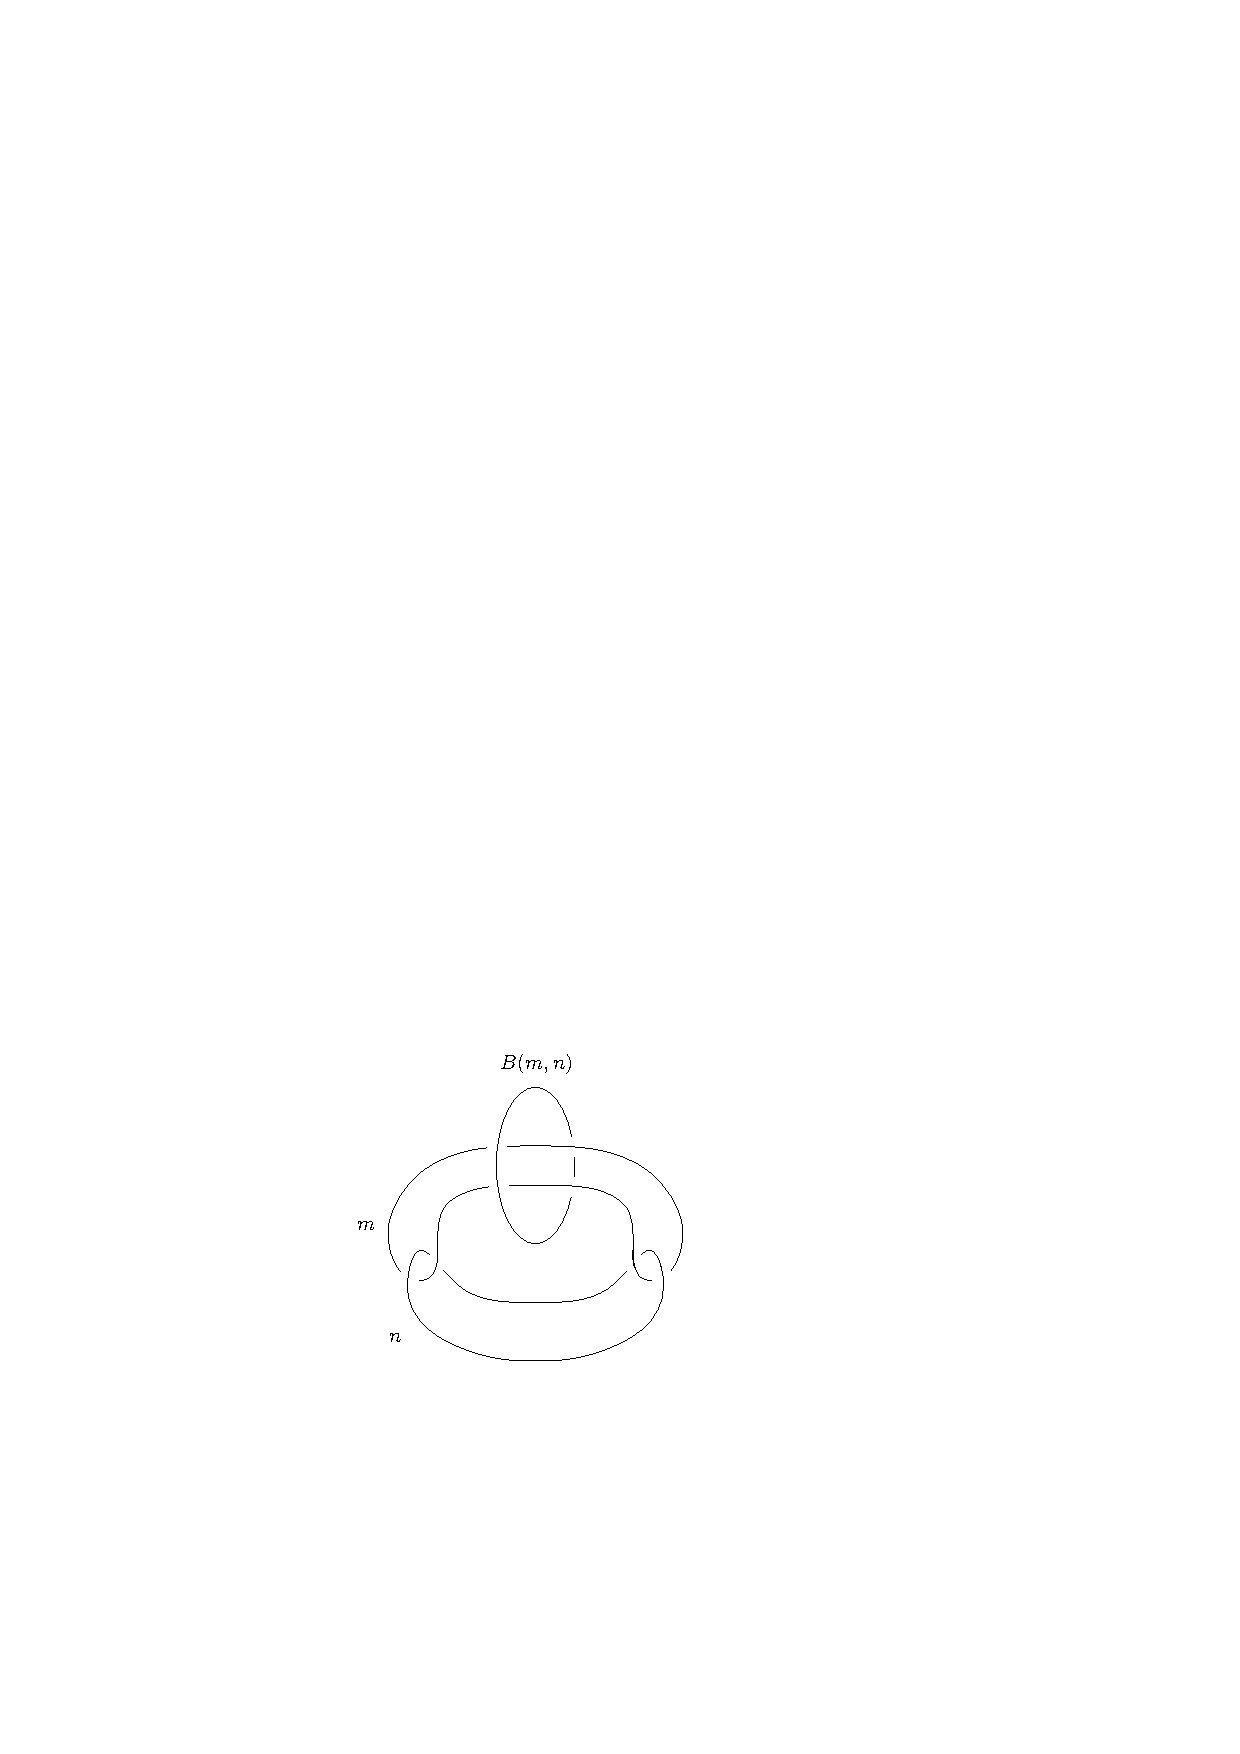
\includegraphics[scale=1]{graphics/knot-B(m,n)}
\caption{The knot $B(m,n)$ in $L(m,1) \# L(n,1)$}
\label{Borromean knot}
\end{figure}

\begin{figure}[p]
\centering
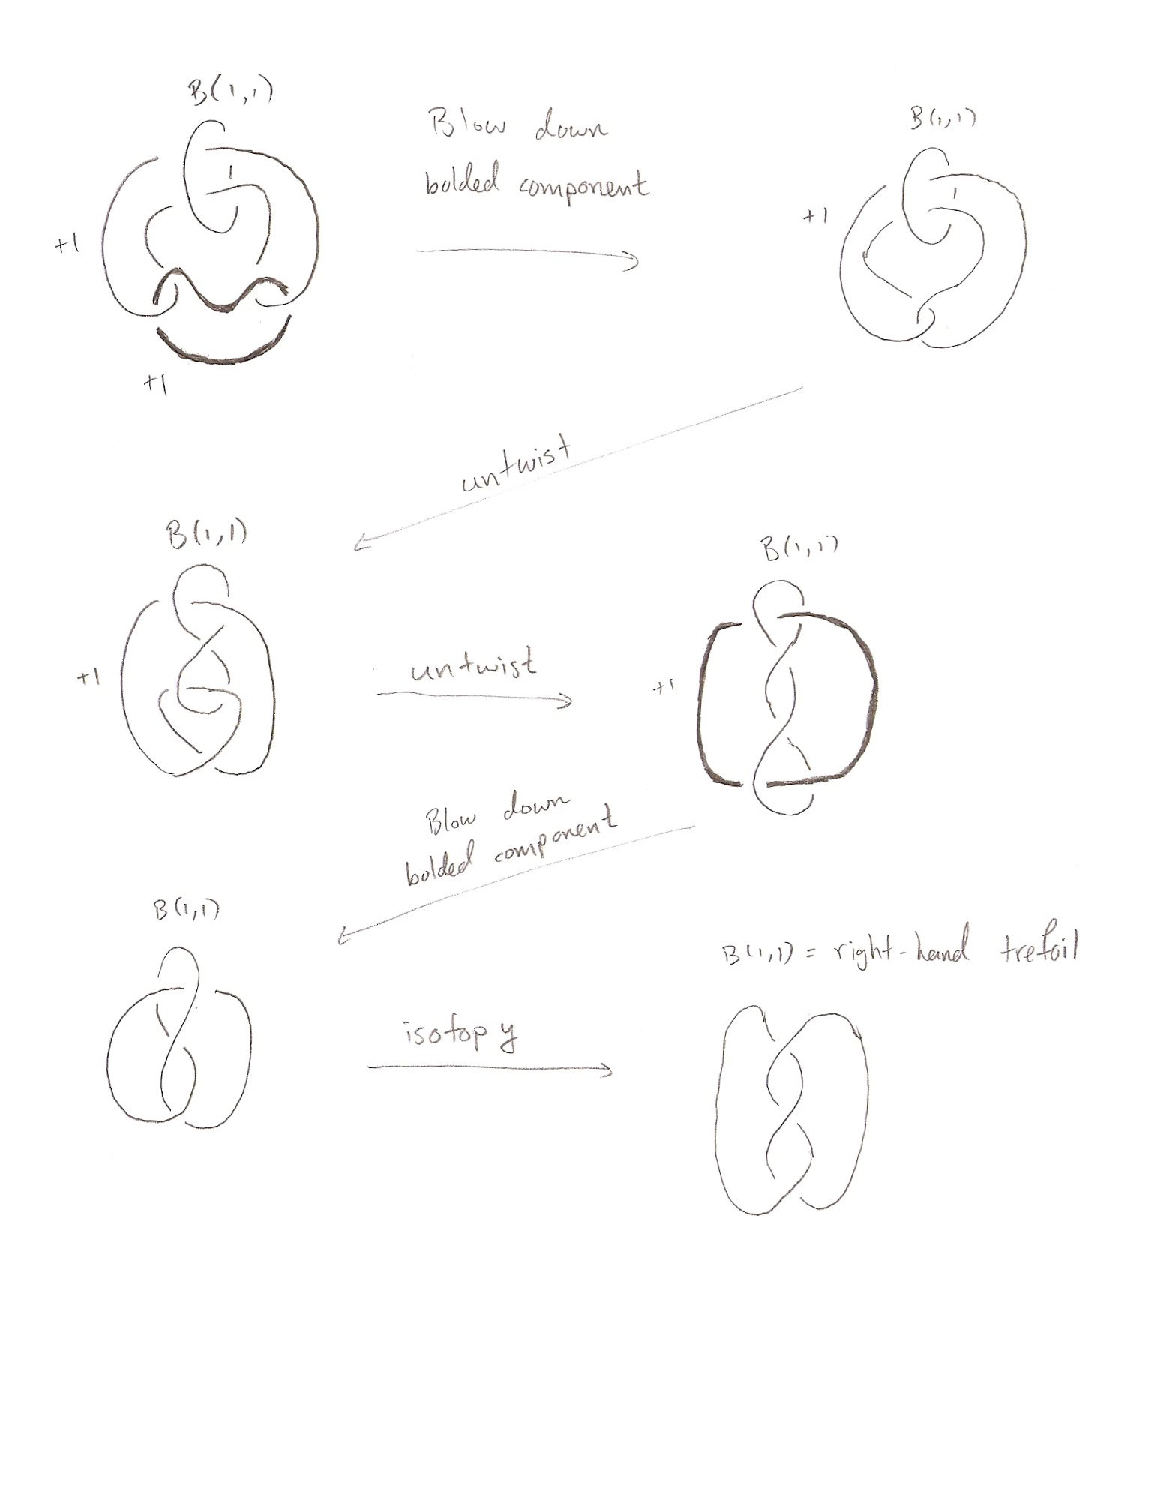
\includegraphics[scale=1]{graphics/borromean-knot-trefoil}
\caption{Using Kirby calculus to show that $B(1,1)$ is the right-handed trefoil}
\label{borromean-knot-trefoil}
\end{figure}

\end{example}

\begin{example}
Similar to the computation in the above example, except working a littler harder, one can show that the knot $B(0,0)$ in $\#2 S^1 \times S^2$ has the following Floer homology
\[ \widehat{HFK}_i(\#2 S^1 \times S^2,B(0,0),j) \cong \begin{cases} \mathbb Z/2 & (i,j)=(1,1),(-1,-1) \\ (\mathbb Z/2)^2 & (i,j)=(0,0) \\ 0 & \text{otherwise} \end{cases} \]
\end{example}


For an oriented link $L$ in $S^3$, let $L_+,L_-,L_0$ denote the oriented links that are the same as $L$ except in the vicinity of a crossing, in which case $L_+,L_-,L_0$ have that crossing changed to a positive, negative or oriented smoothing, respectively (see \cref{skein-links}). If $L$ has $m$ components, then $L_+$ and $L_-$ will also have $m$ components, but $L_0$ will have $m+1$ components. In order to talk about the Floer homology of the links $L_+$ and $L_-$ we look at their associated knots in the space $\# (m-1) S^1 \times S^2$, whereas the associated knot of the link $L_0$ lives in $\# m S^1 \times S^2$. Let $\gamma$ be an unknot placed around a crossing of $L$ such that $L$ intersects the spanning disc of $\gamma$ in a pair of canceling points, and both strands at this crossing belong to the same link component. The link $L_-$ sitting inside the space $S_1^3(\gamma)$ is isotopic to $L_+$ sitting in $S^3$. We claim that $L_-$ sitting in $S_0^3(\gamma) \cong S^1 \times S^2$ is isotopic to the link in $S^1 \times S^2$ obtained by attaching a 1-handle to $S^3$ near the smoothing in $L_0$, and then connecting the two components of $L_0$ near the smoothing with a compatibly oriented band going through the 1-handle. This is shown in \cref{visualizing-L0}. With these comments at hand we immediately have the following exact sequence as a consequence of the surgery exact sequence
\[ \cdots \longrightarrow \widehat{HFK}(S^3,L_-,j) \longrightarrow \widehat{HFK}(S^3,L_0,j) \longrightarrow \widehat{HFK}(S^3,L_+,j) \longrightarrow \cdots \]

\begin{figure}[tb]
\centering
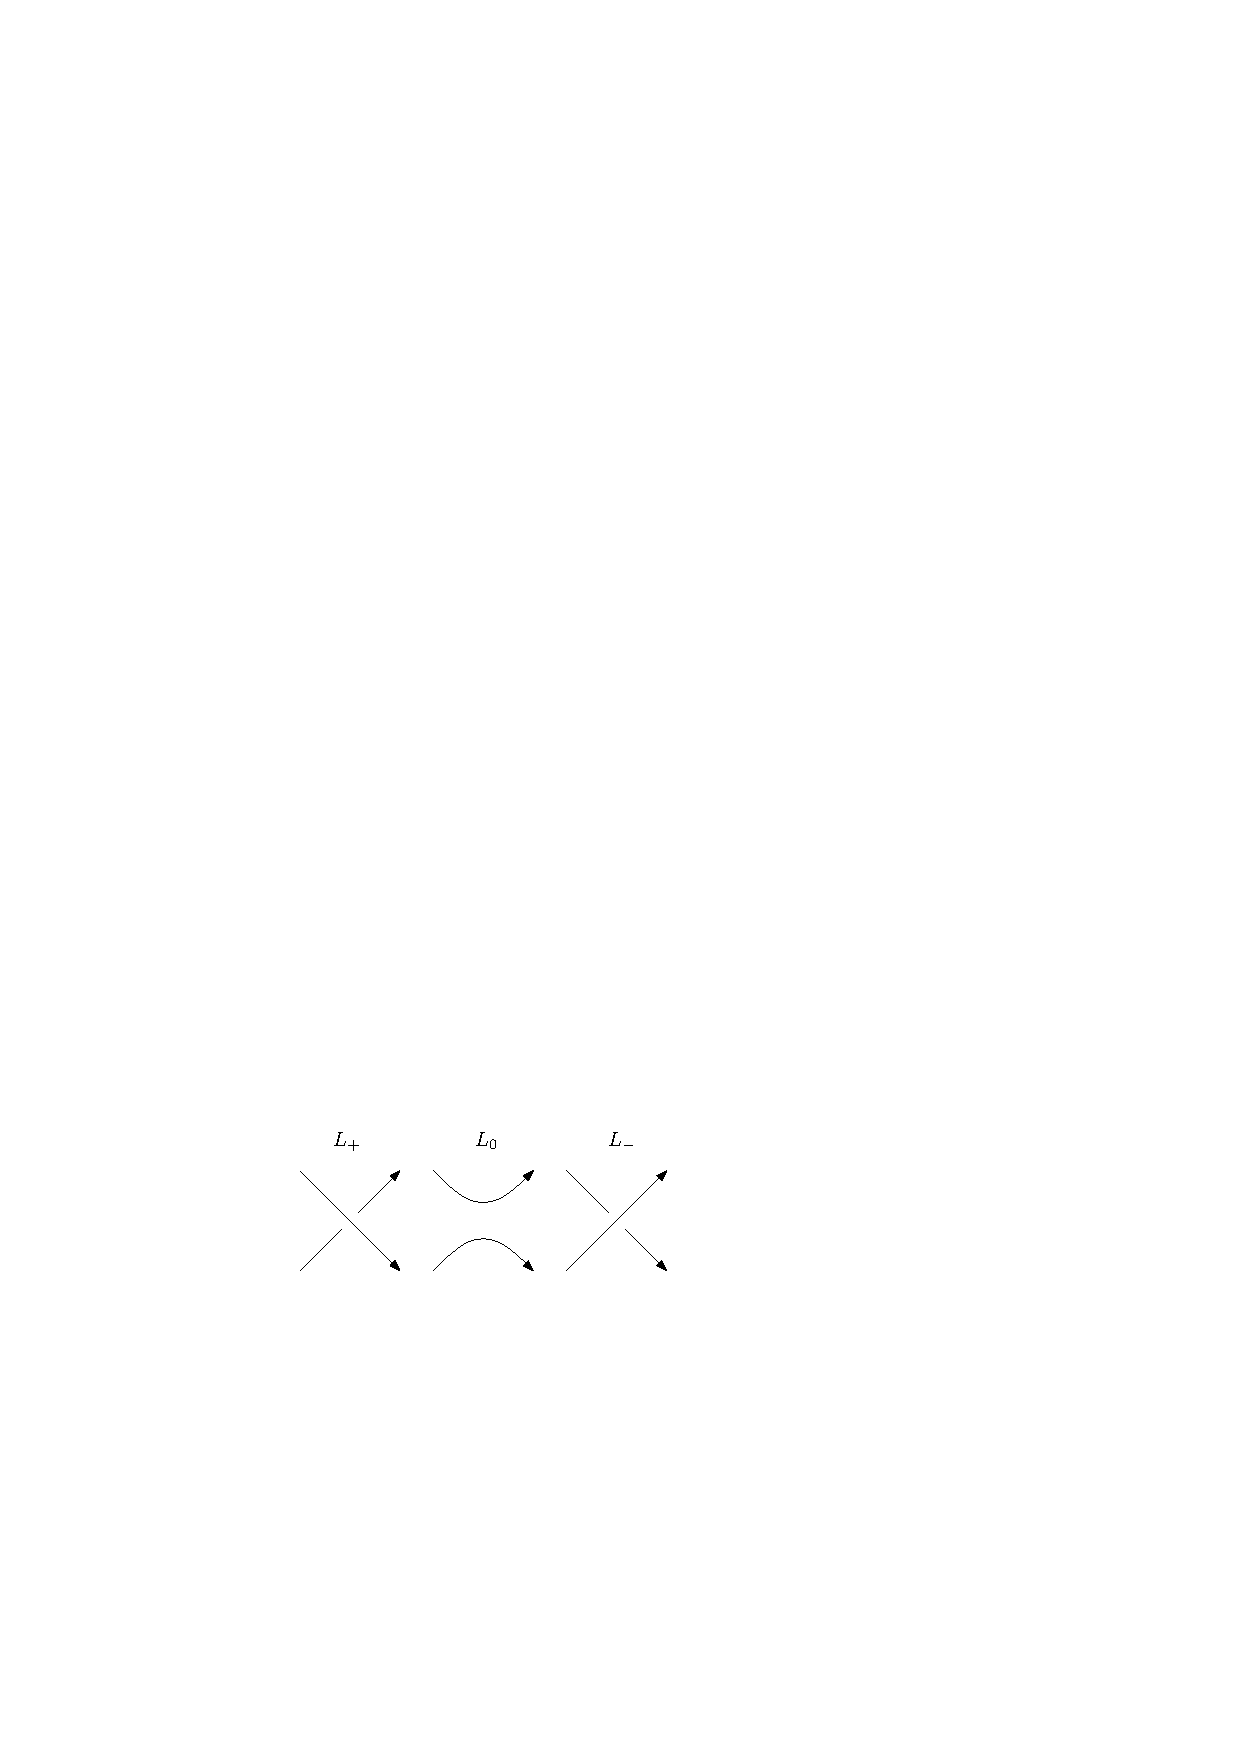
\includegraphics[scale=1]{graphics/skein-links}
\caption{Links in the skein exact sequence}
\label{skein-links}
\end{figure}

\begin{figure}[tb]
\centering
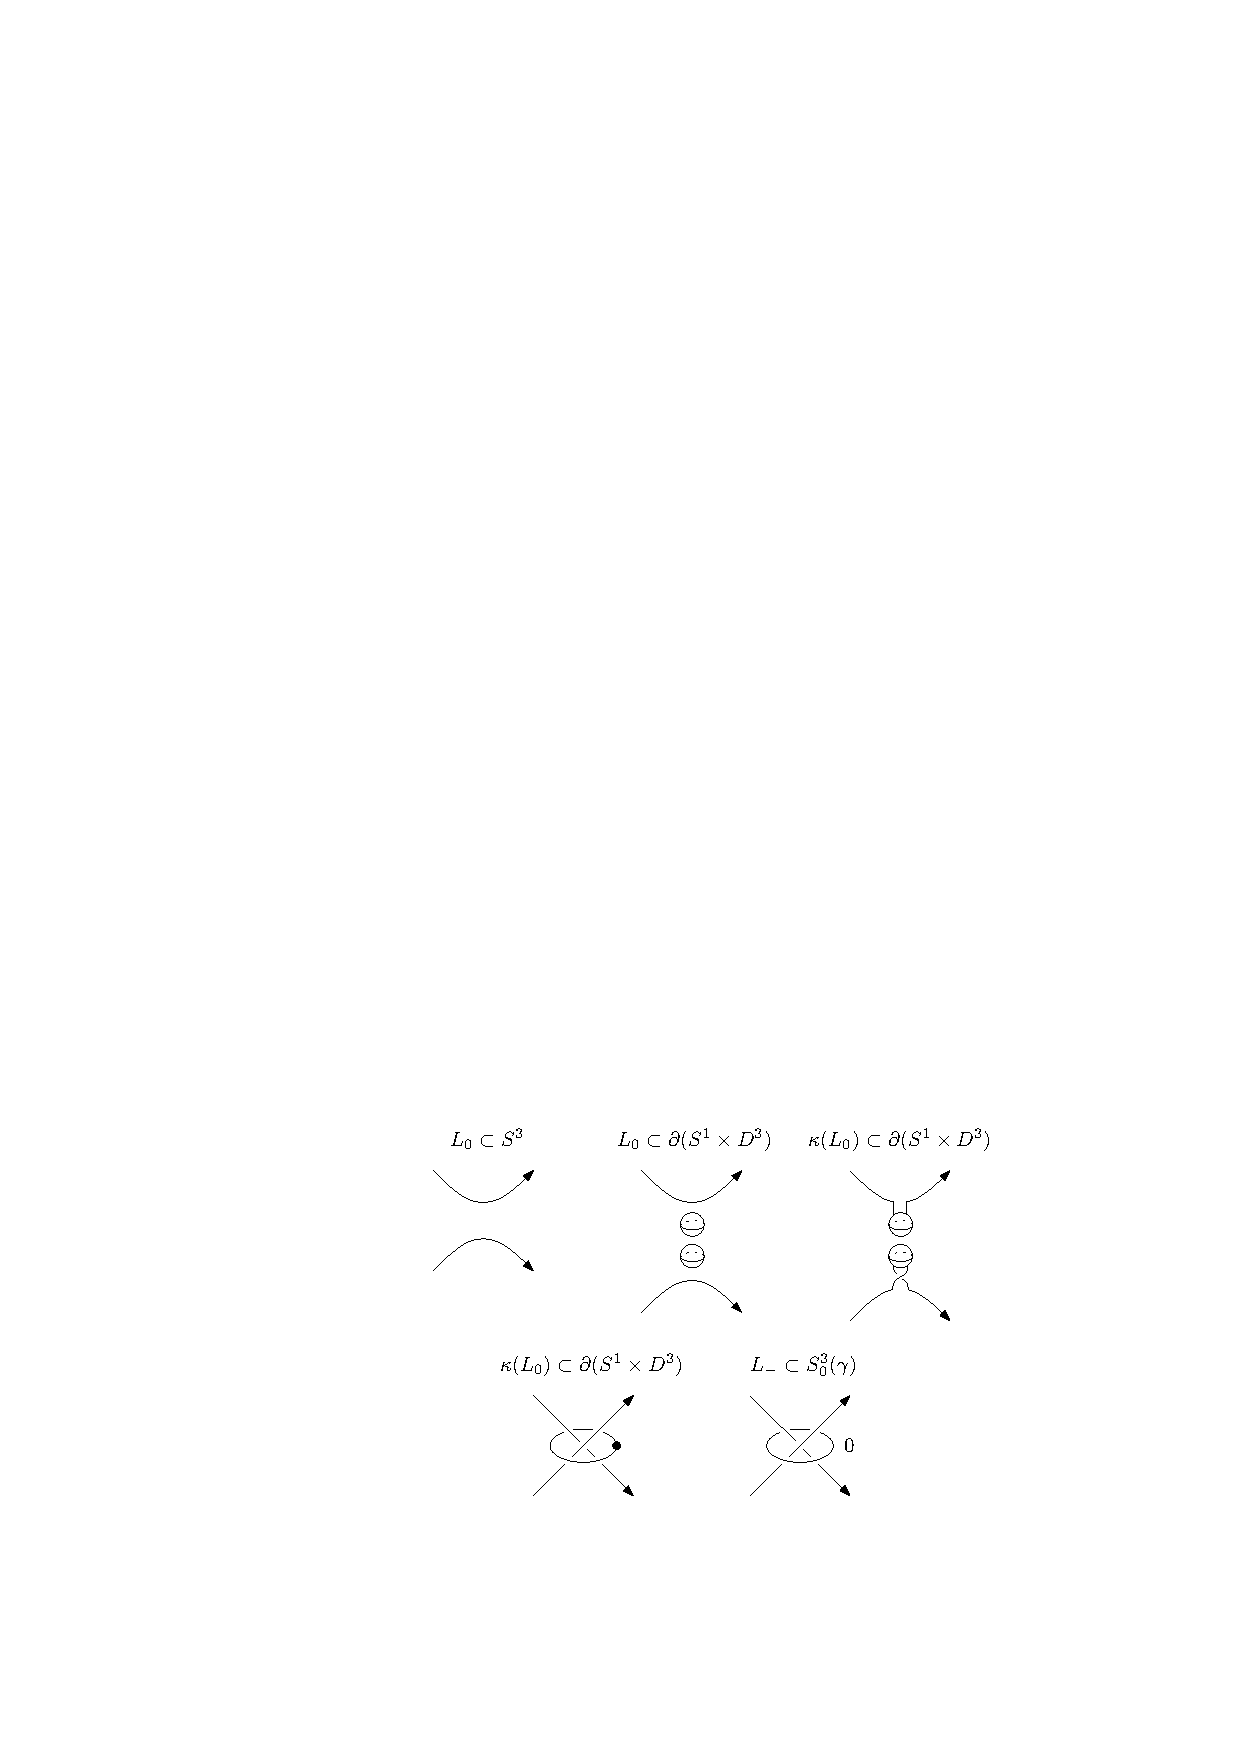
\includegraphics[scale=1]{graphics/visualizing-L0}
\caption{Visualizing $\kappa(L_0)$ in $S^1 \times S^2$ as $L_-$ in $S_0^3(\gamma)$}
\label{visualizing-L0}
\end{figure}

Next we consider a crossing like the above, except now the two strands belong to different components of $L$; in fact, let us assume that $L$ has only two components as the general case can easily be deduced from this. Let $L_-,L_+,L_0$ denote the associated links as in \cref{skein-links}, and let $\gamma$ be an unknot around the crossing such that $L$ intersects its spanning disc in a pair of canceling points. Note that the links $L_-,L_+$ have two components, whereas $L_0$ has one component, and hence is a knot. 


.... \unfinished



In conclusion, we have the following theorem (stated here in more generality):
\begin{thm}[Skein Exact Sequence]
\label{Skein Exact Sequence}
Let $L_-,L_+,L_0$ be three links in $Y$ related by the skein moves. If both strands corresponding to the crossing being changed belong to the same link component, then for each integer $j$ there is an exact sequence of the form
\[ \cdots \longrightarrow \widehat{HFK}(Y,L_-,j) \longrightarrow \widehat{HFK}(Y,L_0,j) \longrightarrow \widehat{HFK}(Y,L_+,j) \longrightarrow \cdots \]
whereas if the strands belong to different components there is an exact sequence of the form
\[ \cdots \longrightarrow \widehat{HFK}(Y,L_-,j) \longrightarrow \widehat{HFK}(Y',L_0',j) \longrightarrow \widehat{HFK}(Y,L_+,j) \longrightarrow \cdots \]
where $(Y',L_0')$ is the connect sum of $(Y,L_0)$ with the knot $(\#2 S^1 \times S^2, B(0,0))$. In particular, in the latter case we have an exact sequence
\[ \cdots \longrightarrow \widehat{HFK}(Y,L_-,j) \longrightarrow \widehat{HFK}(Y,L_0) \otimes V \longrightarrow \widehat{HFK}(Y,L_+,j) \longrightarrow \cdots \]
where $V = V_- \oplus V_0 \oplus V_+$ is a four-dimensional vector space with $V_\pm$ one-dimensional supported in grading $\pm 1$ and $V_0$ two-dimensional supported in grading 0.
\end{thm}




\subsubsection{An Euler Characteristic Calculation}

The skein exact sequences for Floer knot homology allow us to compute the Euler characteristic of $\widehat{HFK}$, and compare it to a classical knot invariant. 




\subsubsection{Kauffman States and another Euler Characteristic Calculation}





\subsubsection{Some Computations}

We will first explain how to obtain genus 1 Heegaard diagrams for 2-bridge knots, and see that their Floer homology can be computed combinatorially. A 2-bridge knot is a knot $k$ in $S^3$ such that there is a height function $f : S^3 \rightarrow \mathbb R$ such that $f|_k$ has precisely two maxima. 

\unfinished




\begin{example}[The Trefoil Knot]

\begin{figure}[tb]
\centering
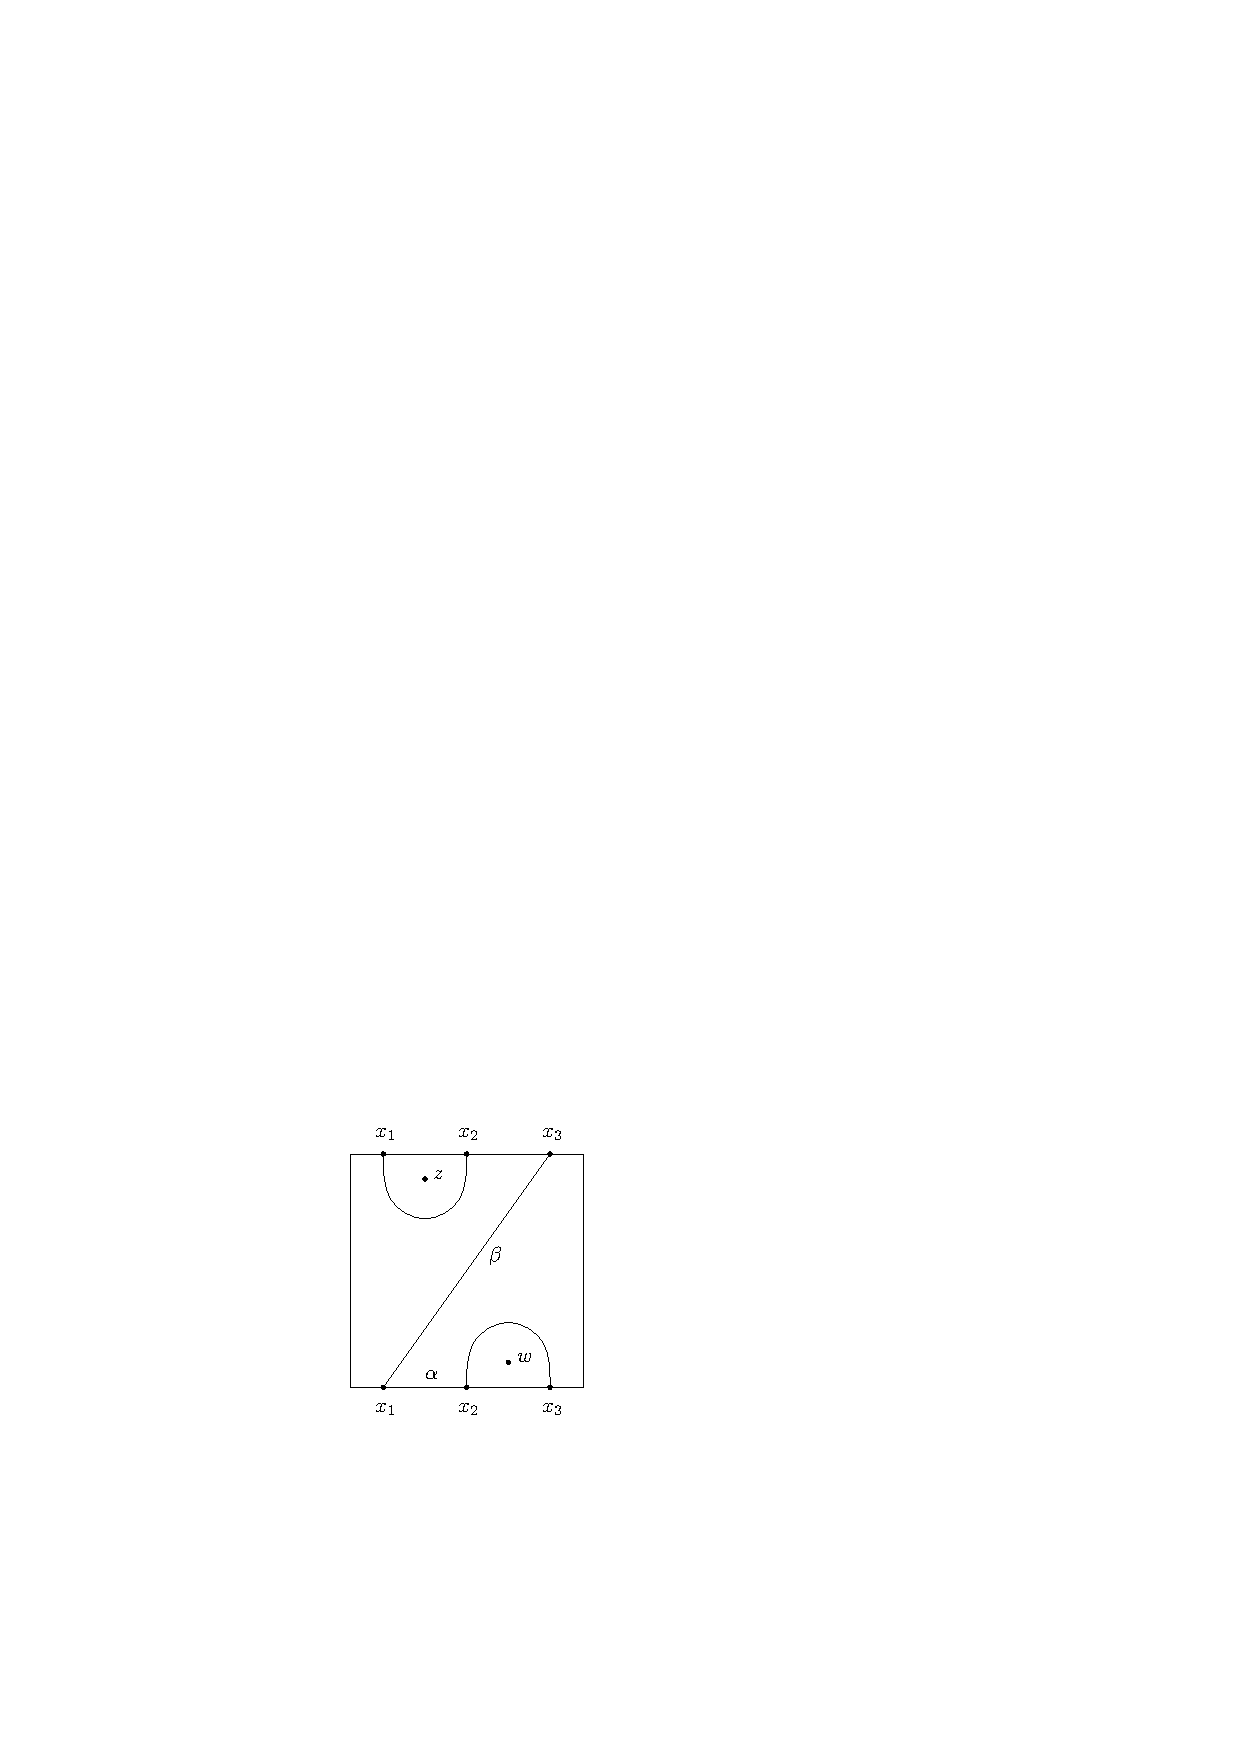
\includegraphics[scale=1]{graphics/trefoil-heegaard-diagram}
\caption{A Heegaard diagram for the trefoil knot}
\label{trefoil-heegaard-diagram}
\end{figure}

\Cref{trefoil-heegaard-diagram} shows a Heegaard diagram for $S^3$ that is compatible with the left-handed trefoil. The intersection points of the $\alpha$ and $\beta$ curves are labelled $x_1,x_2$ and $x_3$. Let us figure out the relative grading of these generators, computed with respect to the base point $w$. For $\gr(x_1,x_2)$ note that we have the obvious disc $\phi_{12}$ which does not intersect $w$ and has a unique holomorphic representative (up to translation), hence $\gr(x_1,x_2)=1$. For $\gr(x_2,x_3)$ we also have the obvious disc $\phi_{23}$, but now the orientations are reversed, so $\mu(\phi_{23})=-1$, and this disc intersects $w$ negatively, hence $\gr(x_2,x_3)=-1-2(-1)=+1$. By additivity of gradings we have $\gr(x_1,x_3)=2$, hence the gradings of the generators differ by one with $x_1$ in the top grading and $x_3$ in the bottom grading. To pin down the translation indeterminacy of this grading we compute the homology of the complex $(\widehat{CF}(\alpha\beta,w)$, which we know is $\mathbb Z/2$ supported in grading zero. In $\partial x_1$ we clearly have the coefficient of $x_2$ is one (we do not need to consider $x_3$ since its grading is too low and $\partial$ lowers gradings by only one). Next we have $\partial x_2=0$ since the disc connecting $x_2$ to $x_3$ does not support a holomorphic representative. Finally we have $\partial x_3=0$ since $x_3$ in the lowest grading. We have now computed $\ker \partial = \< x_2,x_3 \>$ and $\image \partial \< x_2 \>$, hence $\widehat{HF}(\balpha,\bbeta) = \< x_3 \>$, which implies $\gr(x_1)=2,\gr(x_2)=1$ and $\gr(x_3)=0$.

Now let us compute the relative Alexander gradings. Recall that this is defined by $f(\bx,\by)=n_z(\phi)-n_w(\phi)$. For the disc $\phi_{12}$ connecting $x_1$ to $x_2$ we clearly have $f(x_1,x_2)=1$. The disc $\phi_{23}$ connecting $x_2$ to $x_3$ intersects $w$ negatively, hence $f(x_2,x_3)=1$. And by additivity of this grading we have $f(x_1,x_3)=2$. The symmetry property this grading is supposed to have implies that $f(x_1)=1,f(x_2)=0,f(x_3)=-1$. Finally, we compute the homology of $(\widehat{CFK}(\alpha,\beta,z,w),\partial_k)$. However, none of the discs connecting the intersection points miss the points $z$ and $w$, hence the differentials are zero. Therefore $\widehat{HFK}(\alpha,\beta,z,w) = \< x_1,x_2,x_3 \>$, and the gradings look like
\[
\begin{tabular}{|r|c|c|c|}
\hline
$\widehat{HFK}_{ij}$ & $-1$ & $0$ & $1$ \\
\hline
$2$ & & & $\<x_1\>$ \\
\hline
$1$ & & $\<x_2\>$ & \\
\hline
$0$ & $\<x_3\>$ & & \\
\hline
\end{tabular}
\]
It is clear that the Euler characteristic of this bigraded vector space is just the Alexander polynomial: $\Delta_k(t)=t^{-1}-1+t$.
\end{example}




\begin{example}[The Figure Eight Knot]

\begin{figure}[tb]
\centering
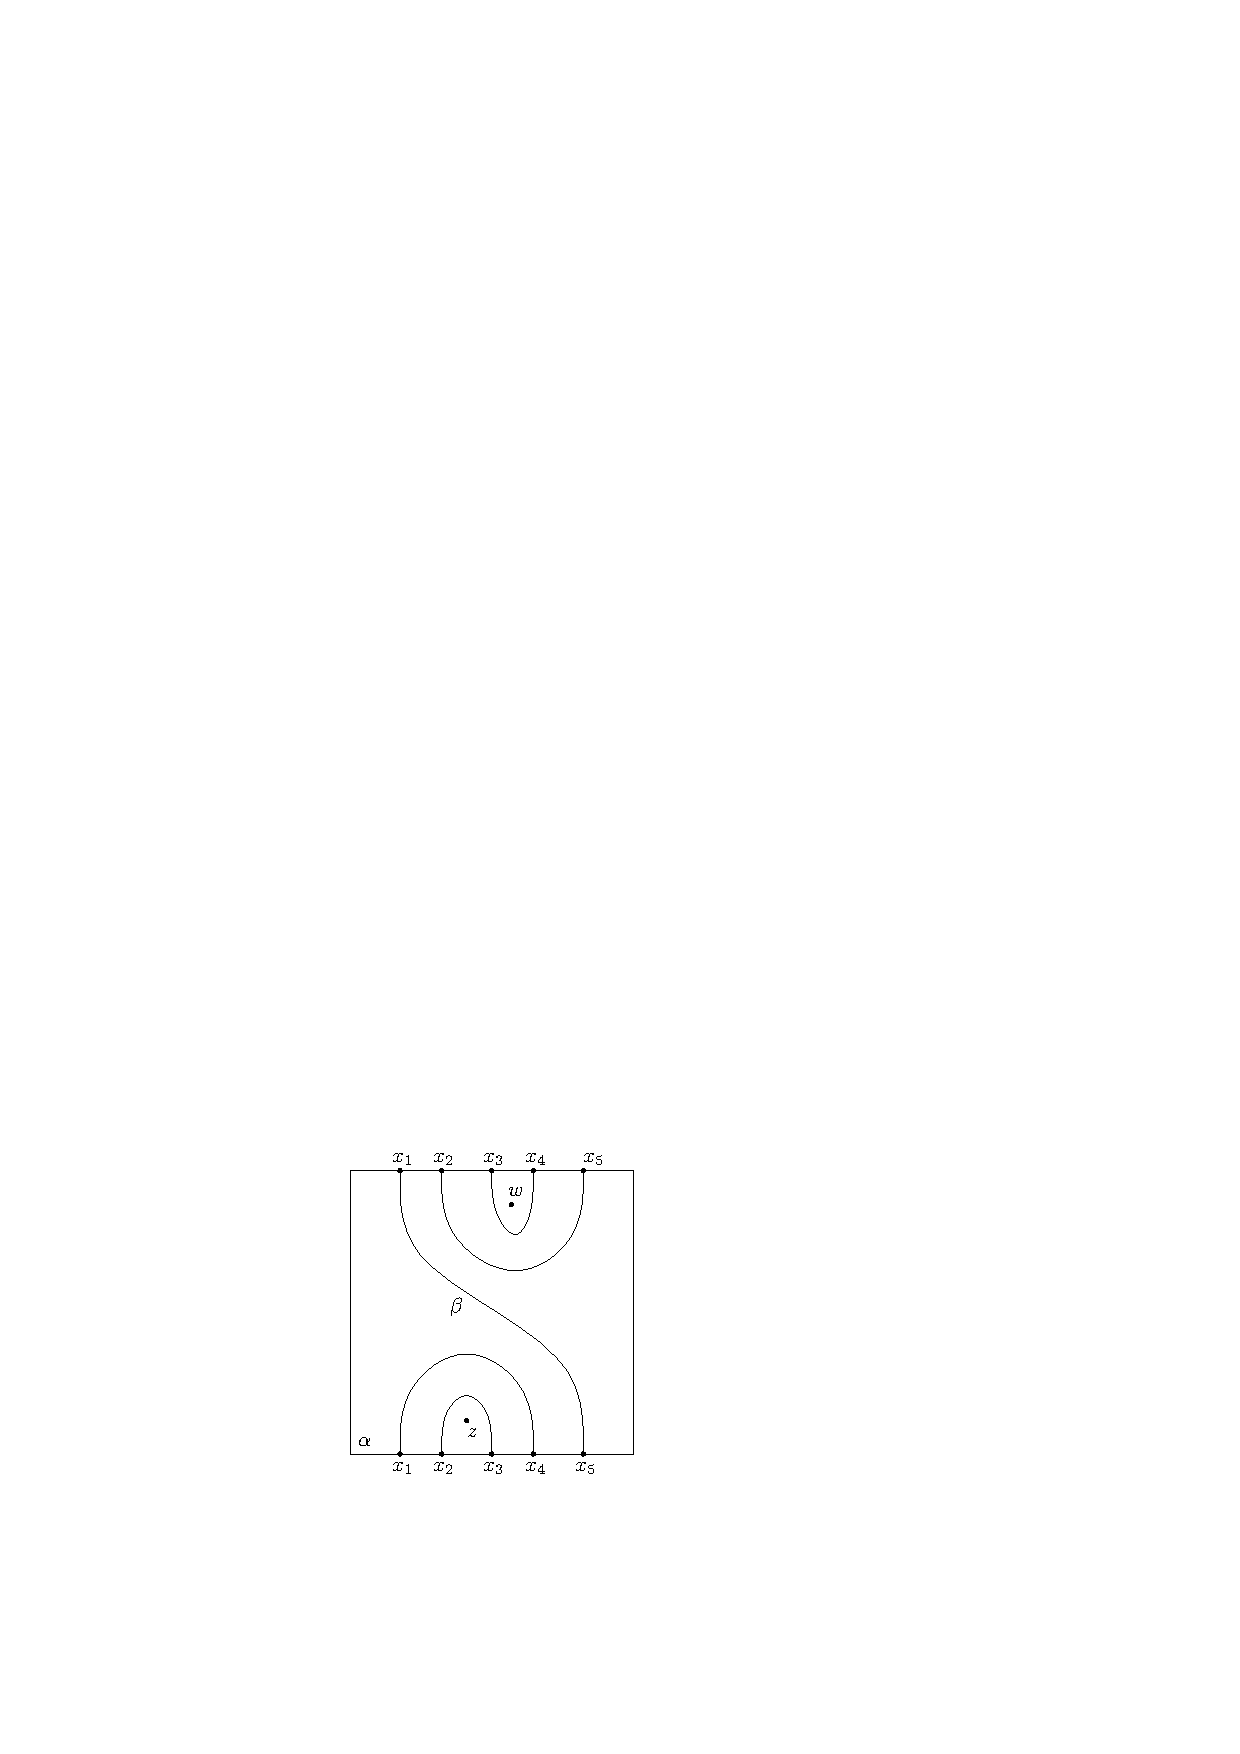
\includegraphics[scale=1]{graphics/figure-eight-heegaard-diagram}
\caption{A Heegaard diagram for the figure eight knot}
\label{figure-eight-heegaard-diagram}
\end{figure}

\Cref{figure-eight-heegaard-diagram} shows a Heegaard diagram for $S^3$ that is compatible with the figure eight knot. Let us first figure out the relative gradings on these generators with respect to the base point $w$. There is a disc connecting $x_1$ to $x_2$ and it intersects $w$ positively, so $\gr(x_1,x_2)=-1$. The obvious disc connecting $x_2$ to $x_3$ does not intersect $w$, and so $\gr(x_2,x_3) = 1$. The obvious disc connecting $x_3$ to $x_4$ has orientations reversed, and so its Maslov index is $-1$ and intersects $w$ negatively, hence $\gr(x_3,x_4) = 1$. Finally, the disc from $x_4$ to $x_5$ has orientations reversed and does not intersect $w$, so $\gr(x_4,x_5)=-1$. To pin down the absolute grading we compute the homology of $(\widehat{CF}(\alpha,\beta,w),\partial)$. The differentials can easily be computed as
\begin{align*}
	\partial x_1 &= x_4 \\
	\partial x_2 &= x_3 \\
	\partial x_3 &= 0 \\
	\partial x_4 &= 0 \\
	\partial x_5 &= x_5 
\end{align*}
Therefore $\ker \partial = \< x_3,x_4,x_1+x_5 \>$ and $\image \partial \< x_3,x_4 \>$, hence $\widehat{HF}(\alpha,\beta,w) = \< x_1+x_5 \>$. This means that $x_1$ and $x_5$ are in grading zero, and so $\gr(x_2)=1,\gr(x_3)=0$ and $\gr(x_4)=-1$. 

Next we compute the relative Alexander gradings. If we just use the discs we used in computing the Maslov grading then we see that the relative Alexander gradings are the same as the relative Maslov gradings. In order for the symmetry property to hold for the maslov gradings we must have $f(x_1)=f(x_3)=f(x_5)=0, f(x_2)=1$ and $f(x_4)$, hence the Alexander gradings are precisely the Maslov gradings. Further, the differential $\partial_k$ on $\widehat{CFK}(\alpha,\beta,z,w)$ is zero, so we have computed $\widehat{HFK}$:
\[
\begin{tabular}{|r|c|c|c|}
\hline
$\widehat{HFK}_{ij}$ & $-1$ & $0$ & $1$ \\
\hline
$1$ & & & $\<x_2\>$ \\
\hline
$0$ & & $\<x_1,x_3,x_5\>$ & \\
\hline
$-1$ & $\<x_4\>$ & & \\
\hline
\end{tabular}
\]
It is clear that the Euler characteristic of this bigraded vector space is the Alexander polynomial of the figure eight: $\Delta_k(t) = t^{-1}-3+t$.
\end{example}








\begin{example}[A Knot with 5 Crossings]

\begin{figure}[tb]
\centering
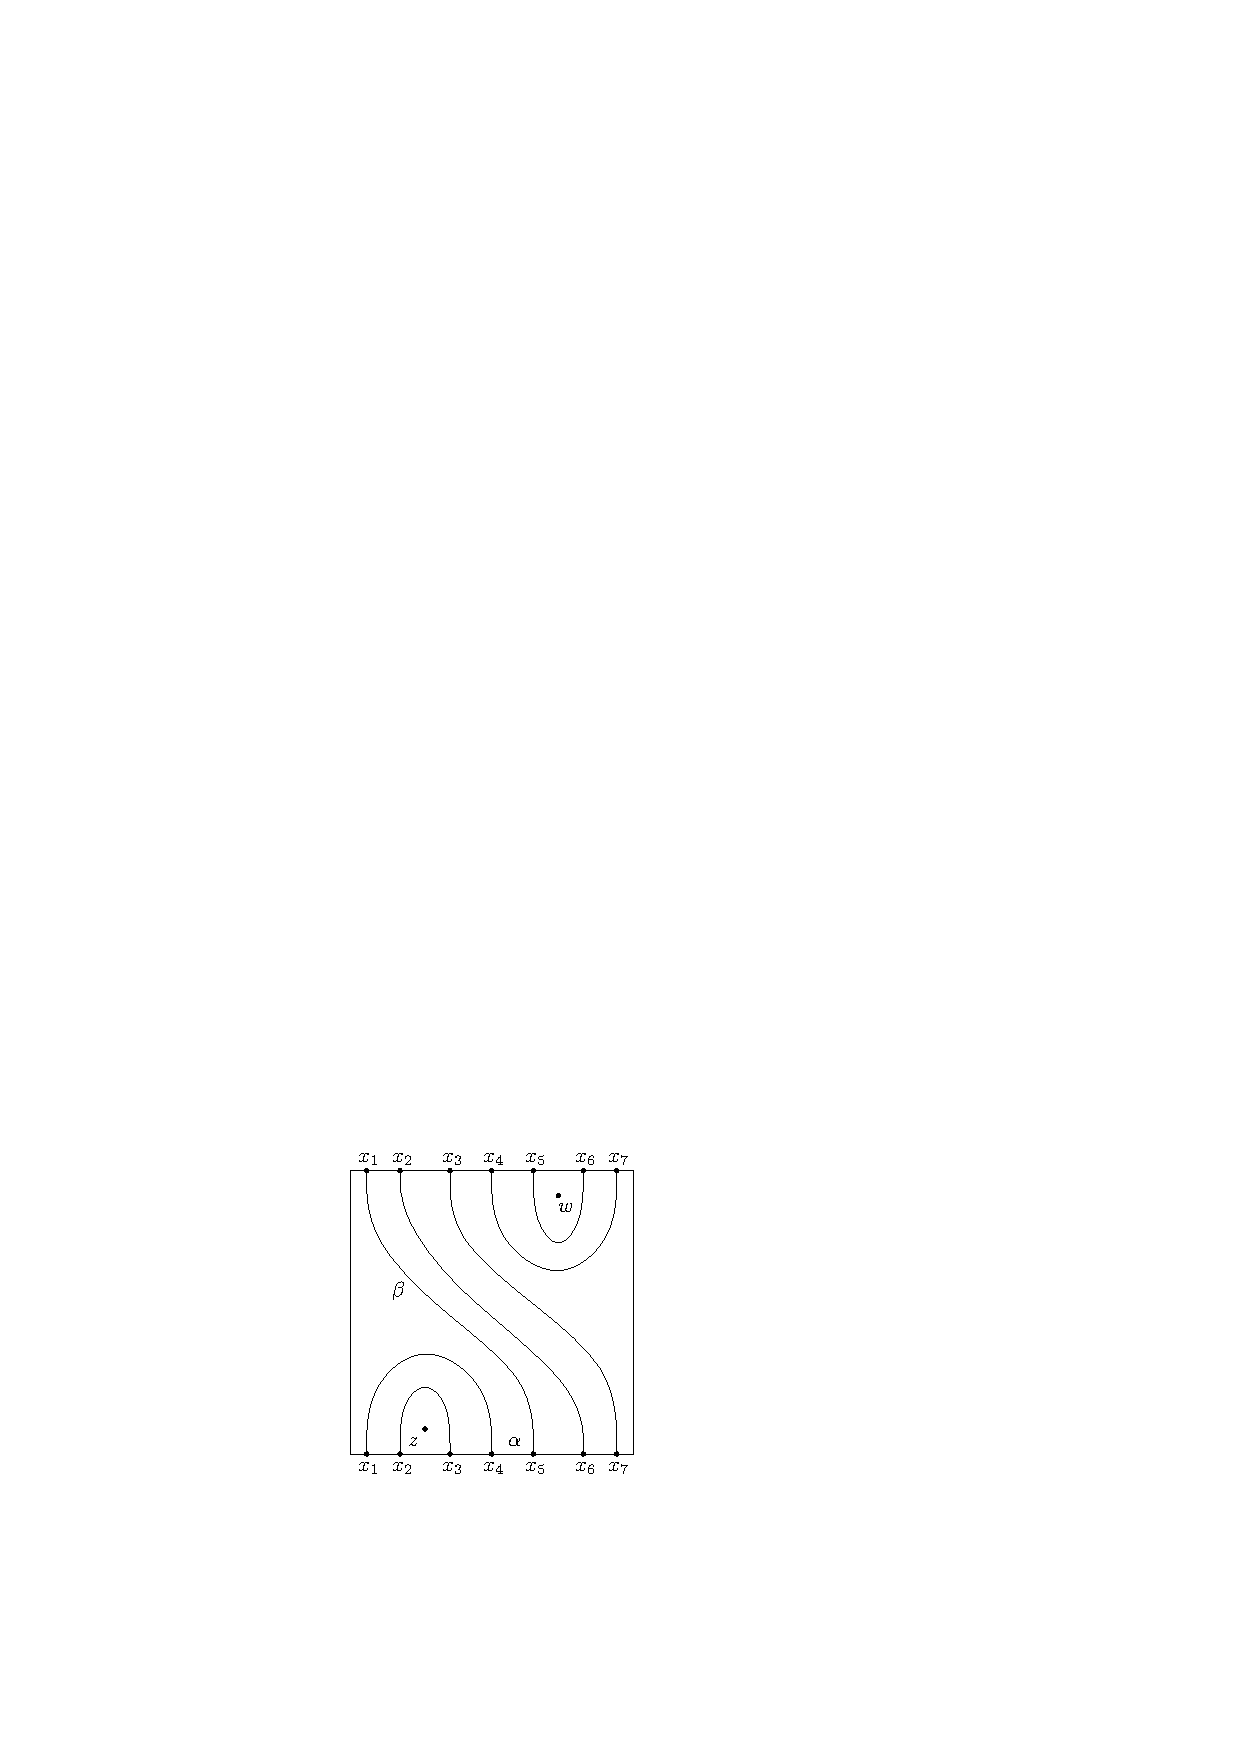
\includegraphics[scale=1]{graphics/5-2-heegaard-diagram}
\caption{A Heegaard diagram for the knot $5_2$}
\label{5-2-heegaard-diagram}
\end{figure}

\Cref{5-2-heegaard-diagram} shows a Heegaard diagram for $S^3$ that is compatible with the $5_2$ knot (a figure eight knot with an extra twist). Let us first figure out the relative gradings on these generators with respect to the base point $w$. There is a disc connecting $x_1$ to $x_2$ that does not intersect $w$, so we have $\gr(x_1,x_2)=1$, and similarly $\gr(x_2,x_3)=1$. However, the disc connecting $x_3$ to $x_4$ passes through $w$ positively, and so $\gr(x_3,x_4)=-1$. Continuing this we can easily compute
\[
\begin{array}{lll}
\gr(x_1,x_2) = 1 & \gr(x_2,x_3) = 1 & \gr(x_3,x_4) = -1 \\
\gr(x_4,x_5) = -1 & \gr(x_5,x_6) = 1 & \gr(x_6,x_7) = 1 
\end{array}
\]
Next we compute the homology of $(\widehat{CF}(\alpha,\beta,w),\partial)$ so that we can figure out the absolute gradings of our generators. We can compute the differentials to be:
\[
\begin{array}{rl}
	\partial x_1 &= x_2 + x_4 + x_6 \\
	\partial x_2 &= x_3 \\
	\partial x_3 &= 0 \\
	\partial x_4 &= x_3 + x_7 \\
	\partial x_5 &= x_2 + x_4 + x_6 \\
	\partial x_6 &= x_7 \\
	\partial x_7 &= 0
\end{array}
\]
It is easy to see that the kernel of $\partial$ is 4 dimensional, generated by $x_3,x_7,x_1+x_5,x_2+x_4+x_6$, while its image is 3 dimensional, generated by $x_3,x_7,x_2+x_4+x_6$. Therefore $\widehat{HF}(\alpha,\beta,w)$ is generated by $x_1+x_5$, and so has absolute grading 0. As a consequence we have $\gr(x_1)=\gr(x_5)=0, \gr(x_2)=\gr(x_4)=\gr(x_6)=-1$ and $\gr(x_3)=\gr(x_7)=-2$.

Now let us compute the Alexander gradings. We can use the same discs we used to compute the Maslov gradings. In particular, the disc from $x_1$ to $x_2$ intersects $z$ positively but misses $w$, hence $f(x_1,x_2)=1$, and similarly $f(x_2,x_3)=1$. The disc from $x_3$ to $x_4$ intersects $w$ positively, but misses $z$, hence $f(x_3,x_4)=-1$. The disc from $x_4$ to $x_5$ intersects $z$ negative and misses $w$, so $f(x_4,x_5)=-1$. The disc from $x_5$ to $x_6$ intersects $w$ negatively and misses $z$, so $f(x_5,x_6)=1$. Finally, the disc from $x_6$ to $x_7$ intersects $z$ positively, and so $f(x_6,x_7)=1$. So, the relative Alexander gradings are equal to the relative Maslov gradings:
\[
\begin{array}{lll}
f(x_1,x_2) = 1 & f(x_2,x_3) = 1 & f(x_3,x_4) = -1 \\
f(x_4,x_5) = -1 & f(x_5,x_6) = 1 & f(x_6,x_7) = 1 
\end{array}
\]
In particular, $x_1,x_5$ are in the same grading, $x_2,x_4,x_6$ are in the same grading, and $x_3,x_7$ are in the same grading. By the symmetry property of the Alexander grading we are forced to have $f(x_1)=f(x_5)=1$, $f(x_2)=f(x_4)=f(x_6)=0$ and $f(x_3)=f(x_7)=-1$. Further, the differential $\partial_k$ on $\widehat{CFK}(\alpha,\beta,z,w)$ is trivial since all discs intersect either $z$ or $w$, and so we have computed $\widehat{HFK}$:
\[
\begin{tabular}{|r|c|c|c|}
\hline
$\widehat{HFK}_{ij}$ & $-1$ & $0$ & $1$ \\
\hline
$0$ & & & $\<x_1,x_5\>$ \\
\hline
$-1$ & & $\<x_2,x_4,x_6\>$ & \\
\hline
$-2$ & $\<x_3,x_7\>$ & & \\
\hline
\end{tabular}
\]
It is clear that the Euler characteristic of this bigraded vector space is the Alexander polynomial of the $5_2$ knot: $\Delta_k(t) = 2t^{-1}-3+2t$.
\end{example}




















\newpage
\appendix


\section{Homotopy Groups}
\label{Homotopy Groups}


Let us assume that we are working in the ``nice'' category of Hausdorff, compactly generated, non-degenerately based spaces. For based spaces $(X,x_0)$ and $(Y,y_0)$, let $f_1,f_2 : X \rightarrow Y$ be maps (not necessarily based) and $u : I \rightarrow Y$ a path. We say that $f_1$ and $f_2$ are \textbf{freely homotopic along $u$} if there is a homotopy $F : X \times I \rightarrow Y$ from $f_1$ to $f_2$ such that $F(x_0,t) = u(t)$ for all $t \in I$, and we denote this by $f_1 \underset{u}{\sim} f_2$. That is, although we are allowing the base point of $X$ to move during the homotopy, we are restricting it to move along a specific path. If $f_1$ and $f_2$ are based maps, then $u$ is necessarily a loop. Here is a simple lemma to show this definition makes sense.

\begin{lem}
\sloppyspace
\begin{enumerate}
	\item For any map $f_1 : X \rightarrow Y$ and path $u : (I,0) \rightarrow (Y,f_1(x_0))$ there is a map $f_2 : X \rightarrow Y$ such that $f_1 \underset{u}{\sim} f_2$.
	\item If $f_1 \underset{u}{\sim} f_2$, $f_1 \underset{v}{\sim} f_3$ and $u \sim v \rel \lcb 0,1 \rcb$, then $f_1 \underset{\text{const}}{\sim} f_3$.
	\item If $f_1 \underset{u}{\sim} f_2$ and $f_2 \underset{v}{\sim} f_3$, then $f_1 \underset{v * u}{\sim} f_3$.
\end{enumerate}
\end{lem}
\begin{proof}
\sloppyspace
\begin{enumerate}
	\item By definition of non-degenerately based we have that $(X,x_0)$ is a fibration. Therefore the homotopy extension problem $f_1 \cup u : X \times \lcb 0 \rcb \cup \lcb x_0 \rcb \times I \rightarrow Y$ can be solved to give a map $F : X \times I \rightarrow Y$ with the desired properties.
	\item 
\end{enumerate}
\end{proof}

This lemma gives us an action of $\pi_1(Y,y_0)$ on the based homotopy classes $[X,Y]_*$: for $[f] \in [X,Y]_*$ and $[u] \in \pi_1(Y,y_0)$, let $[u] \cdot [f] = [g]$, where $g$ is any map such that $f \underset{u}{\sim} g$. This is well-defined by the above lemma.

\begin{prop}
If $Y$ is path connected, then the forgetful map $[X,Y]_* \rightarrow [X,Y]$ descends to a bijection $[X,Y]_* / \pi_1(Y,y_0) \rightarrow [X,Y]$. If $Y$ is simply connected, then the forgetful map is bijective.
\end{prop}







\newpage
\section{Duality Theorems}
\label{Duality Theorems}

\begin{thm}[Poincar\'{e} Duality]
\label{Poincare Duality}
If $M$ a closed, oriented $n$-manifold with fundamental class $[M] \in H_n(M;\mathbb Z)$, then the homomorphism
\[ PD : H^p(M;\mathbb Z) \rightarrow H_{n-p}(M;\mathbb Z) \]
defined by $\alpha \mapsto \alpha \smallfrown [M]$ is an isomorphism.
\end{thm}

This isomorphism is called the \textbf{Poincar\'{e} isomorphism}. It is natural in the sense that if $f : M \rightarrow N$ is a map of closed, oriented manifolds such that $f_*[M] = [N]$, then the following diagram commutes
\[
\xymatrix
@R=3pc
@C=3pc
{
	H^p(M;\mathbb Z) \ar[r]^-{PD} & H_{n-p}(M;\mathbb Z) \ar[d]^{f_*} \\
	H^p(N;\mathbb Z) \ar[r]_-{PD} \ar[u]^{f^*} & H_{n-p}(N;\mathbb Z)
}
\]
The duality isomorphism leads to a bilinear pairing
\[ H^p(M;\mathbb Z) \otimes H^{n-p}(M;\mathbb Z) \rightarrow \mathbb Z \]
which is non-degenerate

We can drop the orientability assumption and get a $\mathbb Z/2$-form of Poincar\'{e} duality.
\begin{thm}
If $M$ is a closed $n$-manifold with a $\mathbb Z/2$-orientation given by $[M] \in H_n(M;\mathbb Z/2)$, then the homomorphism
\[ PD : H^p(M;\mathbb Z/2) \rightarrow H_{n-p}(M;\mathbb Z/2) \]
defined by $\alpha \mapsto \alpha \smallfrown [M]$ is an isomorphism.
\end{thm}

We can also extend these duality theorems to manifolds with boundary.
\begin{thm}[Poincar\'{e}-Lefschetz Duality]
\label{Poincare-Lefschetz Duality}
Let $M$ be a compact, oriented $n$-manifold with boundary with fundamental class $[M,\partial M] \in H_n(M,\partial M;\mathbb Z)$. Then the homomorphisms
\[ PD : H^p(M,\partial M;\mathbb Z) \rightarrow H_{n-p}(M;\mathbb Z) \]
\[ PD : H^p(M;\mathbb Z) \rightarrow H_{n-p}(M,\partial M;\mathbb Z) \]
given by capping homology classes with $[M,\partial M]$ are isomorphisms.
\end{thm}

Finally, a more general form of duality is Alexander duality.
\begin{thm}[Alexander Duality]
\label{Alexander Duality}
Let $X$ be a closed subset of $S^n$ which is a CW complex. Then
\[ \tilde H^i(S^n \backslash X) \cong \tilde H_{n-i-1}(X) \]
\end{thm}






\newpage
\section{Cohomology with Homotopy}
\label{Cohomology with Homotopy}

There is a way of dealing with cohomology classes in terms of homotopy classes of maps. Recall that an \textbf{Eilenberg-MacLane} space of type $(G,n)$ (where $G$ is abelian if $G \geq 2$) is a CW-complex $K(G,n)$ such that $\pi_i(K(G,n)) = G$ if $i=n$ and $0$ otherwise. Hurewicz's theorem implies that $H_i(K(G,n)) = 0$ for all $i < n$ and $H_n(K(G,n)) = G$, and so the exact sequence from the universal coefficient theorem gives a \emph{natural} isomorphism
\[ H^n(K(G,n);G) \cong \Hom(H_n(K(G,n)),G) \cong \Hom(G,G) \]
Let $\iota \in H^n(K(G,n);G)$ denote the cohomology class associated to $\id : G \rightarrow G$ in the above isomorphisms. Then each homotopy class of map $f : X \rightarrow K(G,n)$ gives a cohomology class $f^*\iota \in H^n(X;G)$. This association turns out to be a \emph{natural} isomorphism of abelian groups
\[ [X,K(G,n)] \cong H^n(X;G) \]
where $[X,K(G,n)]$ is given the canonical group structure from the $H$-group structure on $K(G,n) = \Omega K(G,n-1)$. Naturality of the isomorphism means that for any map $f : X \rightarrow Y$ the following diagram commutes
\[
\xymatrix
{
	[X,K(G,n)] \ar[d]_\cong & [Y,K(G,n)] \ar[d]^\cong \ar[l]_-{f^*} \\
	H^n(X;G) & H^n(Y;G) \ar[l]^-{f^*}
}
\]
where $f^*$ denotes the induced map both on the homotopy class of maps and on cohomology.

In the special case of $n=2$ and $G=\mathbb Z$ we get another view of cohomology. The 2nd degree cohomology $H^2(X;\mathbb Z)$ is isomorphic to $[X,K(\mathbb Z)] = [X,\mathbb CP^\infty]$. But, at the same time, the classifying space of $U(1)$ is $BU(1) = \mathbb CP^\infty$, and so $[X,\mathbb CP^\infty]$ is in one-to-one correspondence with complex line bundles over $X$. So each cohomology class $\alpha \in H^2(X;\mathbb Z)$ corresponds to a complex line bundle $L_\alpha \rightarrow X$.





\newpage
\section{Homeomorphisms of Surfaces}
\label{Homeomorphisms of Surfaces}


When constructing combinatorial pictures of 3-manifolds it will be useful to know something about self-homeomorphisms of surfaces. We will be gluing together manifolds with boundary equal to a surface of genus $g$ along a self-homeomorphism of that surface, so in particular we only need to know self-homeomorphisms of surfaces \emph{up to isotopy}. This motivates the definition of the mapping class group. For any manifold $M$, let $\Homeo(M)$ denote the group of orientation preserving, self-homeomorphisms of $M$, and let $\Homeo_0(M)$ denote the normal subgroup of $\Homeo(M)$ that are isotopic to the identity. The quotient $H(M) = \Homeo(M) / \Homeo_0(M)$ is called the mapping class group of $M$. 

The structure of $H(M)$ is usually quite complicated, but in the case of the torus we have a simple description of its mapping class group, and for a general surface we have an explicit set of generators. Let $\Sigma$ be a surface of genus $g$, and let $c$ be an embedded circle in $\Sigma$. Associated to this curve there are 2 elements of $H(\Sigma)$, which are inverses of each other, called  the Dehn twists along $c$. Take a small tubular neighborhood $N(c)$ of $c$ in $\Sigma$. Since $N(c)$ is an annulus, let $\varphi : N(c) \rightarrow A$ be a homeomorphism onto the standard annulus $A = \lcb z \st 1 \leq |z| \leq 2 \rcb$ such that $\varphi(c) = \lcb z \st |z|=2 \rcb$. Then define the homeomorphism $\tau_c : \Sigma \rightarrow \Sigma$ by
\[ \tau(x) = \begin{cases} x & x \notin N(c) \\ \varphi^{-1}\left( \varphi(x) \cdot e^{2\pi i (|\varphi(x)|-1)} \right) & x \in N(c) \end{cases} \]
This determines an element of $H(\Sigma)$, and had we twisted in the other direction we would have gotten the inverse to the above element. Further Dehn twists around isotopic curves are isotopic.

There is a standard family of $3g$ embedded curves on a surface $\Sigma$ of genus $g$, label them by $\alpha_i,\beta_i,\gamma_j$ for $i=1,\ldots,g$ and $j=1,\ldots,g-1$. 
\begin{thm}[Dehn-Lickorish]
\label{Dehn-Lickorish Theorem}
The group $H(M)$ is generated by Dehn twists along the curves $\alpha_i,\beta_i,\gamma_i$.
\end{thm}

\Cref{Dehn-Lickorish Theorem} gives us an explicit description of the mapping class group of the torus. Let $T = S^1 \times S^1$ be the 2-torus. Let $\mu = S^1 \times \lcb 1 \rcb$ and $\lambda = \lcb 1 \rcb \times S^1$ be the standard meridian and longitude on $T$. A homeomorphism $f : T \rightarrow T$ induces an isomorphism $f_* : \pi_1(T) \rightarrow \pi_1(T)$, where $\pi_1(T) = \mathbb Z \oplus \mathbb Z$ is generated by $\mu$ and $\lambda$. Every automorphism of $\mathbb Z \oplus \mathbb Z$ is given by an integer-valued matrix whose determinant is $\pm 1$. If $f$ is orientation preserving, then the matrix representation of $f_*$ has determinant $+1$. Further, isotopic homeomorphisms induce the same map on homology, hence we have a homomorphism
\begin{equation}
\label{torus mapping class group isomorphism}
\Phi : H(T) \longrightarrow \SL(2,\mathbb Z)
\end{equation}
\begin{prop}
The map $\Phi$ is an isomorphism.
\end{prop}
\begin{proof}
We will only show the surjective part of this proposition. Any matrix $A \in \SL(2,\mathbb Z)$ can be reduced to the identity by composing with elementary transformations. Over the integers these transformations are of the form
\[ \begin{pmatrix} 1 & \pm 1 \\ 0 & 1 \end{pmatrix} \ \ \ \ \ \ \ \begin{pmatrix} 1 & 0 \\ \pm 1 & 1 \end{pmatrix} \]
Under the isomorphism \eqref{torus mapping class group isomorphism} these matrices correspond to Dehn twists around $\mu$ and $\lambda$, which we know generates $H(T)$ by \cref{Dehn-Lickorish Theorem}. Therefore $\Phi$ is surjective.
\end{proof}






\newpage
\section{Some Analysis}
\label{Some Analysis}


Let $V$ and $W$ be Banach spaces and $f : V \rightarrow W$ a map. We say that $f$ is a differentiable at a point $v \in V$ if there is a bounded linear map $df_v : V \rightarrow W$ such that
\[ \lim_{h \to 0} \frac{ \norm{f(v+h)-f(v)-df_v(h)} }{ \norm{h} } = 0 \]
We call $df_v$ the derivative of $f$ at $v$. If $df_v$ exists for all $v \in V$ we obtain a map $df : V \rightarrow L(V,W)$, where $L(V,W)$ is the Banach space of bounded linear maps $V \rightarrow W$ given the operator norm: for $L \in L(V,W)$ we set $\norm{L} = \sup \lcb \norm{L(v)} \st v \in V, \norm{v} \leq 1 \rcb$. Since $L(V,W)$ is another Banach space we can discuss the differentiable properties of $df$. In general, we say that $f$ is of class $C^1$ if $f$ is differentiable and $df$ is continuous (i.e. bounded), and inductively say that $f$ is of class $C^k$ if $df$ is of class $C^{k-1}$. 

A $C^k$ Banach manifold modeled on a Banach space $V$ is a topological space $X$ with a cover $\lcb U_\alpha \rcb$ and collection of charts $x_\alpha : U_\alpha \rightarrow E$ which are bijections onto the open set $x_{\alpha}(U_\alpha)$ such that for any two charts $(x_\alpha,U_\alpha)$ and $(x_\beta,U_\beta)$ we have that $x_\beta \circ x_{\alpha}^{-1} : x_{\alpha}(U_\alpha \cap U_\beta) \rightarrow x_\beta(U_\alpha \cap x_\beta)$ is $C^k$ as a map between open sets of the Banach space $E$. If we speak of just \emph{Banach manifolds}, and leave out its $C^k$ class, then we take the manifold to be $C^\infty$. We can develop the notions of tangent vectors and differentials in the same way as finite dimensional manifolds.

\begin{thm}[Implicit Function Theorem]
Let $f : X \rightarrow Y$ be a $C^k$ map between Banach manifolds. If $y \in Y$ is a regular value, then $f^{-1}(y)$ is a $C^k$ submanifold of $X$ and $T_x f^{-1}(y) = \ker df_x$ for all $x \in f^{-1}(y)$.
\end{thm}

A linear map $T : V \rightarrow W$ between Banach spaces is said to be \textbf{Fredholm} if the kernel and cokernel of $T$ are finite dimensional, and the image of $T$ is closed in $W$. Such maps are our best chance at transferring problems in the infinite dimensional setting to the finite dimensional world. The \textbf{index} of a Fredholm operator is defined to be $\ind(T) = \dim\ker T - \dim\coker T$. The space of Fredholm operators $F(V,W)$ forms an open set in $L(V,W)$, and the index function $\ind : F(V,W) \rightarrow \mathbb Z$ is locally constant.

Let $X$ be a topological space and $P(x)$ a statement which evaluates to true or false for each $x \in X$. We say that $P(x)$ is true for \textbf{generic} $x \in X$ if the solution set $\lcb x \in X \st P(x) \rcb$ contains a countable intersection of open dense sets. The infinite dimensional version of Sard's theorem can now be stated.
\begin{thm}[Sard-Smale]
Let $X$ and $Y$ be separable Banach manifolds. Let $f : X \rightarrow Y$ be a $C^k$ map such that $df_x : T_x X \rightarrow T_{f(x)} Y$ is Fredholm of index $l$ for all $x \in X$. Assume $k \geq 1$ and $k \geq l+1$. Then a generic $y \in Y$ is a regular value of $f$, i.e. $df_x$ is onto for all $x \in f^{-1}(y)$.
\end{thm}

Let $X$ be a Banach manifold modeled on $V$ and $E$ another Banach manifold. A smooth surjective map $\pi : E \rightarrow X$ of Banach manifolds is said to be a Banach $W$-bundle (with $W$ a Banach space) if $X$ is equipped with a covering $\lcb U_\alpha \rcb$ and smooth charts $\varphi_\alpha : \pi^{-1}(U_\alpha) \rightarrow U_\alpha \times U_\alpha \times W$ such that for any two $\varphi_\alpha,\varphi_\beta$ we have $\varphi_\beta \circ \varphi_\beta : (U_\alpha \cap U_\beta) \times W \rightarrow (U_\alpha \cap U_\beta) \times W$ is of the form $(p,w) \mapsto (p,g(p)(w))$, where $g : U_\alpha \cap U_\beta \rightarrow GL(W)$ is smooth (here $GL(W)$ is the group of topological linear isomorphisms $W \rightarrow W$). This implies that each fiber $E_x := \pi^{-1}(x)$ has the structure of a Banach space, which is isomorphic to $W$ but not in any canonical way. We denote the zero section (i.e. all of the zero vectors) of $E$ by $0_E$.

Let $\pi : E \rightarrow X$ be a Banach $W$-bundle, and let us write the elements of $E$ as pairs $(x,e) \in X \times E$ where $\pi(e)=x$. The tangent space of $E$ at a point $(x,0)$ in the zero section naturally splits as
\[ T_{(x,0)} E = T_x X \oplus E_x \]
For a point $x \in X$ let $\pi_x : T_{(x,0)} E \rightarrow E_x$ be the projection onto the second factor. If $s : X \rightarrow E$ is a section ($\pi \circ s = \id$) and let $x \in X$ be a point such that $s(x)=0$. Then using the natural identification above we define the \emph{vertical part} of the differential $ds$ to be the composition $Ds_x := \pi_x \circ ds_x : T_x X \rightarrow E_x$ (we use a capital $D$ for the vertical differential and a lower case $d$ for the regular differential). The following result is very useful.
\begin{thm}
\label{useful Banach bundle result}
Let $X$ and $Y$ be separable Banach manifolds, $E \rightarrow X \times Y$ a Banach bundle, and $s : X \times Y \rightarrow E$ a smooth section. If for each $(x,y) \in s^{-1}(0_E)$ we have
\begin{enumerate}
	\item The vertical differential $Ds_{(x,y)} : T_{(x,y)}(X \times Y) \rightarrow E_{(x,y)}$ is surjective.
	\item The vertical differential $Ds_{(x,y)}$ restricted to $T_y Y$ is Fredholm of index $k$.
\end{enumerate}
Then for generic $x \in Y$, the set $\lcb y \in Y : s(x,y)=0 \rcb$ is a $k$-dimensional submanifold of $Y$. Further, the restriction of $Ds_{(x,y)}$ to $T_y Y$ is surjective.
\end{thm}
\begin{proof}
By the first condition on $s$ we already have that $s^{-1}(0_E)$ is a Banach submanifold of $X \times Y$ by the inverse function theorem. Let $\pi : X \times Y \rightarrow X$ be the projection onto the first factor. Let $(x,y) \in X \times Y$ such that $s(x,y) = 0$. Then, as we remarked before, the tangent space at $(x,y,0)$ in $E$ splits as $T_{(x,y,0)} E = T_x X \oplus T_y Y \oplus E_{(x,y)}$, and so the vertical differential is given by $Ds_{(x,y)} = \pi_{(x,y)} \circ ds_{(x,y)}$, where $\pi_{(x,y)}$ is the projection of $T_{(x,y,0)}$ onto $E_{(x,y)}$. 

\unfinished

\comment{
, and consider the restriction of $\pi$ to $s^{-1}(0_E)$. First we show that for $(x,y) \in s^{-1}(0_E)$ the differential $d\pi_{(x,y)}$ is Fredholm of index $k$. 

As we remarked before, the tangent space at a point in the zero section of $E$ splits as $T_{(x,y,0)} E = T_x X \oplus T_y Y \oplus E_{(x,y)}$. So, the vertical differential is given by $Ds_{(x,y)} = \pi_{(x,y)} \circ ds_{(x,y)}$
}

\end{proof}



For a region $U \subseteq \mathbb R^n$ we define $L^p(U)$ to be the space of functions $f : U \rightarrow \mathbb R$ such that
\[ \norm{f}_p := \left( \int_U |f|^p \right)^{1/p} < \infty \]
If $f \in L^p([a,b])$ we say that $g \in L^p([a,b])$ is the \textbf{weak derivative} of $f$ if for every $\phi \in C^1([a,b])$ with $\phi(a)=\phi(b)=0$ we have
\[ \int_a^b f\phi' = -\int_a^b g\phi \]
More generally, if $f \in L^p(U)$ and $\alpha$ is a multi-index, then we say that $g \in L^p(U)$ is the $\alpha$-th weak derivative of $f$ if for every $\phi \in C_c^1(U)$ we have
\[ \int_U f D^\alpha \phi = (-1)^{|\alpha|} \int_U g\phi \]
where $D^\alpha = \pfrac{^{|\alpha|}}{x^{\alpha_1} \cdots \partial x^{\alpha_k}}$ is the $\alpha$-th differential operator. Weak derivatives are unique (up to a set of measure zero), and if a function is already differentiable then its weak derivative is equal to its regular derivative. Therefore we also denote the weak derivative by $D^\alpha f$, or just $f'$ for $U \subset \mathbb R$. We can further generalize this ideal to functions in $L^p(U,\mathbb R^n)$ by defining weak derivatives for each component. The subset of $L^p(U,\mathbb R^n)$ with $k$ weak derivatives in $L^p(U,\mathbb R^n)$ is denoted by $W^{k,p}(U,\mathbb R^n)$. 
\begin{prop}
If $f \in W^{1,2}(U,\mathbb R^n)$ $(U \subseteq \mathbb R)$ such that $f'$ is continuous, then $f \in C^1(U)$.
\end{prop}
\begin{proof}
For a fixed $a \in U$ define $g : U \rightarrow \mathbb R^n$ by
\[ g(x) = \int_a^x f'(t) \, dt \]
Since $f'$ is continuous we have that $g$ is $C^1$. But, then $g'=f'$ and so $g=f$ almost everywhere. Since $W^{1,2}$ embeds into $C^0$ we have that $f$ is continuous, hence $g=f$ \emph{everywhere}, and so $f$ is $C^1$.
\end{proof}


\todo{Sobolev norms, completions and embeddings}




\begin{lem}
Let $X,Y,Z$ be Banach spaces, $D : X \rightarrow Y$ a bounded linear operator and $K : X \rightarrow Z$ a compact linear operator. If there is a constant $C>0$ such that
\[ \norm{x}_X \leq C \left( \norm{Dx}_Y + \norm{Kx}_Z \right) \]
for all $x \in X$, then $D$ has closed range and finite dimensional kernel.
\end{lem}
\begin{proof}

\end{proof}









\newpage
\section{Some Exercises}


\begin{exercise}
Let $k_1,k_2$ be oriented, disjoint knots in $S^3$. The four definitions of $\lk(k_1,k_2)$ presented in these notes are equivalent.
\end{exercise}
\begin{proof}[Solution]
\sloppyspace
\begin{enumerate}
	\item Let $\mu_1$ be a meridian of $k_1$ and $F_2$ be an oriented Seifert surface of $k_2$. Perturb $F_2$ slightly, if necessary, so that $k_1$ and $F_2$ intersect transversally in the interior of $F_2$. We claim that the integer $L$ such that $[k_2] = L [\mu_1]$ is precisely $k_1 \cdot F_2$. 
\end{enumerate}
\end{proof}



\begin{exercise}
If $\overline{k}$ denotes the mirror of $k$, then $\Delta_k(t) = \Delta_{\overline k}(t)$.
\end{exercise}
\begin{proof}[Solution]
Suppose $\overline k$ is the reflection of $k$ through a plane $\Pi$ in $\mathbb R^3$. If $F$ is a Seifert surface of $k$, then let $\overline F$ denote the Seifert surface of $\overline k$ obtained by reflecting through $\Pi$. If $x_1,\ldots,x_{2g}$ are generators for $H_1(F)$, then let $\overline x_1,\ldots,\overline x_{2g}$ denote their reflections, and these generate $H_1(\overline F)$. We have the relation
\[ \lk(x_i,x_j^+) = -\lk(\overline x_i,\overline x_j^+) \]
therefore $\overline S = -S$. So, 
\[ \Delta_{\overline k}(t) = \det(t^{1/2}\overline S-t^{-1/2}\overline S^T) = \det(-(t^{1/2}S-t^{-1/2}S^T)) = \Delta_k(t) \]
\end{proof}



\begin{exercise}
$\Delta_{k_1 \# k_2}(t) = \Delta_{k_1}(t) \cdot \Delta_{k_2}(t)$
\end{exercise}
\begin{proof}
If $F_1,F_2$ are Seifert surfaces for $k_1,k_2$ respectively, then $F_1 \sharp F_2$ is a Seifert surface for $k_1 \# k_2$. We clearly have $H_1(F_1 \sharp F_2) \cong H_1(F_1) \oplus H_1(F_2)$, so if we pick bases $\alpha = \lcb x_1,\ldots,x_{2g} \rcb$ and $\beta = \lcb y_1,\ldots,y_{2g} \rcb$ for $H_1(F_1)$ and $H_1(F_2)$ we can take their union to get a basis for $H_1(F_1 \sharp F_2)$. Further, the push-offs of the $\alpha$ basis elements do not link the the $\beta$ elements, and vice-versa, so the Seifert matrix $S$ with respect to this basis is $S_1 \oplus S_2$, where $S_i$ is the Seifert matrix of $F_i$. Therefore $\Delta_{k_1 \# k_2}(t) = \Delta_{k_1}(t) \cdot \Delta_{k_2}(t)$.
\end{proof}



\begin{exercise}
If $k$ is a knot then $\Delta_k(1)=1$, and if $L$ is a link with more than one component then $\Delta_L(1)=0$.
\end{exercise}
\begin{proof}
If $S$ is a Seifert matrix of some Seifert surface of $k$ with respect to some basis, then $\Delta_k(1) = \det(S-S^T)$. The $(i,j)$-entry of $S-S^T$ is $\lk(x_i,x_j^+)-\lk(x_j,x_i^+) = \lk(x_i,x_j^+)+\lk(x_i,x_j^-) = x_i \cdot x_j$. So, $S-S^T$ is the matrix of the intersection pairing $\cdot : H_1(F) \otimes H_1(F) \rightarrow \mathbb Z$ in the basis $\lcb x_i \rcb$, which we know is a non-degenerate, anti-symmetric form, and so it is a direct sum of matrices $\begin{pmatrix} 0&1\\-1&0 \end{pmatrix}$ in some basis. The determinant of this matrix is clearly 1, and so it follows $\Delta_k(1)=1$.

We can repeat the same arguments for a link $L$ with more than one component, except now we claim the intersection pairing $\cdot : H_1(F) \otimes H_1(F) \rightarrow \mathbb Z$ is degenerate. If $F$ is a Seifert surface for $L$, then there is a non-trivial 1-cycle $\alpha$ going once around one of the boundary components of $F$ (since $\partial L$ has more than one connected components). However, every embedded curve in $F$ can be isotoped to completely miss the boundary of $F$, hence the intersection product of $\alpha$ with any other cycle is zero, hence the intersection pairing is degenerate. It follows that so the determinant of any matrix representation is 0, hence $\Delta_L(t)=0$.
\end{proof}


\begin{exercise}
The Alexander polynomial is zero for any split link.
\end{exercise}
\begin{proof}
If $k_1$ and $k_2$ are knots in $S^3$ that can be separated by a closed 3-ball, then $F_1 \# F_2$ is a Seifert surface for $k_1 \cup k_2$, where $F_1,F_2$ are Seifert surfaces for $k_1,k_2$ respectively. If $\lcb x_i \rcb$ and $\lcb y_i \rcb$ are bases for $F_1$ and $F_2$ respectively, then $\lcb x_i,y_j,\mu \rcb$ is a basis for $F_1 \# F_2$, where $\mu$ is a meridian of the tube used to connected $F_1$ and $F_2$. This meridian does not link with any of the push-offs of the $x_i$'s and $y_i$'s, and vice-versa, therefore there is an entire column of zeros in $t^{1/2}S-t^{-1/2}S^T$, and so $\Delta_{k_1\cup k_2}(t)=0$.
\end{proof}


\begin{exercise}
Let $L$ be an oriented link, and let $L_+,L_-,L_0$ denote the links obtained from $L$ be changing a fixed crossing to a positive crossing, a negative crossing, or resolving the crossing in an oriented fashion. Then we have the skein relation
\[ \Delta_{L_+}(t) - \Delta_{L_-}(t) = (t^{1/2}-t^{-1/2}) \Delta_{L_0}(t) \]
\end{exercise}
\begin{proof}

\end{proof}



\begin{exercise}
\sloppyspace
\begin{enumerate}
	\item $\sigma(k) = -\sigma(\overline k)$
	\item $\sigma(k_1 \# k_2) = \sigma(k_1) + \sigma(k_2)$
	\item $\sigma(k)$ is even for knots $k$
	\item If $k_1$ and $k_2$ are concordant, then $\sigma(k_1)=\sigma(k_2)$.
\end{enumerate}
\end{exercise}
\begin{proof}
\sloppyspace
\begin{enumerate}
	\item If $S$ is a Seifert matrix for $k$, then $-S$ is a Seifert matrix for $\overline k$, so
	\[ \overline k = \sigma(-S - S^T) = \sigma(-(S+S^T)) = \sigma(S+S^T) = \sigma(k) \]
	
	\item If $S_1,S_2$ are Seifert matrices for $k_1,k_2$, then $S_1 \oplus S_2$ is a Seifert matrix for $k_1 \# k_2$, and so the result follows.
	
	\item First we claim that $\det(S+S^T) \neq 0$ so that $S+S^T$ has no zero eigenvalues. The Alexander polynomial can be written as $\Delta_k(t) = a_0 + a_1(t+t^{-1}) + \cdots + a_n(t^n+t^{-n})$, and since $\Delta_k(1)=1$ we must have $a_0$ is odd, and hence $\det(k) = \det(S+S^T)$ is odd. Since the number of positive eigenvalues plus the number of eigenvalues of $S+S^T$ is equal to $2g$, it follows that their difference is even.
	
	\item Recall that $k_1$ and $k_2$ are said to be concordant if .....
\end{enumerate}
\end{proof}



\begin{exercise}
For a knot $k$ we have $\sign(\Delta_k(-1)) = (-1)^{\sigma(k)/2}$.
\end{exercise}
\begin{proof}
We have $\Delta_k(-1) = \det(S+S^T)$ for some Seifert matrix $S$ of $k$, and the sign of this is the product of the sign of the eigenvalues of $S+S^T$. 
\end{proof}







\newpage


\bibliography{Low-Dimensional-Topology-Bibliography}
\bibliographystyle{plain}
\addcontentsline{toc}{section}{\refname}









\end{document}

